\documentclass[8pt, handout]{beamer} 

%% Math packages
%%
\usepackage{amsmath,amsthm,amssymb}
% Removes the "Too many math alphabets used in version normal" error.
\newcommand\hmmax{0} 
\newcommand\bmmax{0}
\usepackage[new]{old-arrows}
\usepackage{cancel}
\usepackage{mathdots}
\usepackage{venndiagram}
\usepackage{mathrsfs}          % Math script font

% Graphics
%%
\graphicspath{{./}{figs/}}
\usepackage{graphicx}
\usepackage{tikz}
\usetikzlibrary{arrows}
\usetikzlibrary{decorations.markings}
\usetikzlibrary{decorations.pathreplacing}
\usetikzlibrary{patterns}
\usetikzlibrary{shapes.geometric}
\usetikzlibrary{matrix}
\usepackage{tikz-3dplot}
\usepackage{tkz-graph}
\usepackage{tikz-cd}

%% Colors (most are in colors.tex file)
%%
\usepackage{xcolor}
\usepackage{color}
\usepackage{visualalgebra}  %% Put this *after* the TikZ packages
\usepackage{visualalgebraslides}  %% Put this *after* "visualalgebra"

%% Page layout packages
%%
\usepackage{url}
\usepackage{multicol}
\usepackage{multirow}
\usepackage[numbers,square,sort&compress]{natbib}

%% Font and formatting packages
%%
\usepackage[english]{babel}    % Removing this causes compiler error
\usepackage{alltt}             % Like verbatim, but excludes \ and { }
\usepackage{enumerate}         % [shortlabels] option??
\usepackage{comment}
\usepackage{soul}              % strikeout text
\usepackage{bm}                % Bold math
\usepackage[T1]{fontenc}
\usepackage{relsize}

%% Fixes the \mathbf{} not working for fonts under 10pt
\usepackage{cmbright}
\fontencoding{OT1}\fontfamily{cmbr}\selectfont %to load ot1cmbr.fd
\DeclareFontShape{OT1}{cmbr}{bx}{n}{% change bx definition
<->cmbrbx10%
}{}
\normalfont

\makeatletter
\renewcommand*\env@matrix[1][\arraystretch]{%
  \edef\arraystretch{#1}%
  \hskip -\arraycolsep
  \let\@ifnextchar\new@ifnextchar
  \array{*\c@MaxMatrixCols c}}
\makeatother


%%=======================================================================

%% Beamer packages
%%
\mode<presentation>
{
  \usetheme{boadilla} 
  \useinnertheme{rectangles}
  \usecolortheme{dolphin}
}

\setbeamersize{text margin left=6mm}
\setbeamersize{text margin right=6mm}
\setbeamersize{sidebar width right=0mm}
\setbeamersize{sidebar width left=0mm}
\setbeamertemplate{navigation symbols}{}

\def\newblock{\hskip .11em plus .33em minus .07em}

% Other options: ball, circle, square 
\setbeamertemplate{enumerate items}[default]
%\setbeamercolor{enumerate subitem}{fg=red!80!black}
\def\opacity{0.5}
%\setbeamercovered{transparent}
\setbeamercovered{invisible}


\newcommand{\Pause}{}      %% Comment this out => lots more page breaks


\begin{document}


%%====================================================================

\title[A zoo of examples of groups!]{A zoo of examples of groups!}

\author[\href{mailto:sbagley@westminsteru.edu}{S. Bagley}]
       {\href{mailto:sbagley@westminsteru.edu}{Spencer Bagley}}

\institute[Westminster] { 
  \normalsize With many thanks to Matthew Macauley, \\
  \url{http://www.math.clemson.edu/~macaule/}}

\date[29 Jan 2025]{29 Jan 2025}

\frame{\titlepage}

%%====================================================================

\begin{frame}{Families of groups} %\Pause

  So far we've seen some examples of \textit{individual} groups, but here we're going to see some examples of \textit{families} of groups, because they'll be nice go-to examples:

  \begin{enumerate}
  \item \textbf{\Alert{cyclic groups}}: rotational symmetries
  \begin{itemize}
    \item (Side quest: \Alert{orbits} and \Alert{cycle graphs}) \Pause
  \end{itemize}
  \item \textbf{\Alert{dihedral groups}}: rotational \emph{and}
    reflective symmetries \Pause
  \item \textbf{\Alert{abelian groups}}: where $ab=ba$ (always) \Pause
  \item \textbf{\Alert{permutation groups}}: collections of
    rearrangements. \Pause
  \end{enumerate}

  We'll show that \emph{every} finite group is ``isomorphic'' to a
  permutation group. \medskip\Pause

  Then, we'll see how to combine groups into bigger groups using
  
  \begin{enumerate}
    \setcounter{enumi}{5}
  \item \textbf{\Balert{direct products}} and 
  \item \textbf{\Balert{semidirect products}} of groups.  \Pause
  \end{enumerate}

  I'm also kicking a couple of things to the homework for you to think about on your own:

  \begin{enumerate}
    \setcounter{enumi}{7}
    \item \textbf{\Alert{matrix groups}}
    \item the \textbf{\Alert{quaternion group}} $Q_8$
  \end{enumerate}


  
  %efore finishing with a few miscellaneous examples. 
  
\end{frame}

%%====================================================================

\begin{frame}{Some definitions} %\Pause

  \begin{block}{Definition}
    A \Alert{subgroup} of $G$ is a subset $H\subseteq G$ that
    is also a group. We denote this by $H\leq G$.
  \end{block}

  (More on this soon.)

  \bigskip\Pause
  
  \begin{definition}
    The \Alert{order of a group} $G$ is its size as a set 
    (how many distinct elements are in it), denoted by
    $|G|$.
  \end{definition} \Pause

  \begin{example}
    $|\Sq| = 8$, and $|\Z| = \infty$.
  \end{example}

  \bigskip\Pause
  
  \begin{definition}
    The \Alert{order of an element} $g\in G$ is
    $|g|:=\big|\<g\>\big|$, i.e., either \smallskip
    \begin{itemize}
    \item the minimal $k\geq 1$ such that $g^k=e$, or \smallskip
    \item $\infty$, if there is no such $k$.
    \end{itemize}
  \end{definition}
  
\end{frame}

%%====================================================================
%%====================================================================
\section{Cyclic groups}


%%====================================================================

\begin{frame}{Cyclic groups}
  
  \begin{block}{Definition}
    A group is \Alert{cyclic} if it can be generated by a single
    element.
  \end{block}
  
  \smallskip\Pause
  
  \Alert{Finite} cyclic groups describe the symmetries of objects that have
  \emph{only} rotational symmetry.
  %%
  %% Molecules of boric acid
  \[
  \begin{tikzpicture}[scale=.27,auto]
    \tikzstyle{v-r} = [circle, minimum size=3mm, draw, fill=red]
    \tikzstyle{v-b} = [circle, inner sep=0pt, minimum size=2.5mm, draw,
      fill=blue]
    \tikzstyle{v-g} = [circle, inner sep=0pt, minimum size=2mm, draw, 
      fill=green]
    \tikzstyle{bond} = [draw,very thick, faded,line width=4pt]
    %%
    \node (r1) at (0:0) [v-r] {};
    \node (b1) at (60:2) [v-b] {};
    \node (b2) at (180:2) [v-b] {};
    \node (b3) at (300:2) [v-b] {};
    \node (g1) at (35:3) [v-g] {};
    \node (g2) at (155:3) [v-g] {};
    \node (g3) at (275:3) [v-g] {};
    \draw [bond] (r1) -- (b1) -- (g1);
    \draw [bond] (r1) -- (b2) -- (g2);
    \draw [bond] (r1) -- (b3) -- (g3);
  \end{tikzpicture}
  \hspace{15mm}
  
\includegraphics[height=.68in]{pinwheel4.jpg}\hspace{15mm}
  
\includegraphics[height=.68in]{pinwheel10.jpg}
  \]

  \begin{exampleblock}{Remark}
    You can make a cyclic group of any order you want.
  \end{exampleblock}
\end{frame}

%%====================================================================

\begin{frame}[t]{Cyclic groups, multiplicatively}
  
  \begin{definition}
    For $n\geq 1$, the \Alert{multiplicative cyclic group $C_n$} is
    the set
    \[
    C_n=\big\{1,r,r^2,\dots,r^{n-1}\big\},
    \]
    where $r^ir^j=r^{i+j}$, and the exponents are taken modulo
    $n$. The identity is $r^0=r^n=1$.
  \end{definition}
  
  \vspace{-2mm}\Pause

  %% Several Cayley graphs of small cyclic groups, multiplicatively
  \[
  \begin{tikzpicture}[scale=.4,auto]
    \tikzstyle{every node}=[font=\small]
    %%
    \begin{scope}[shift={(0,-.25)}]
      \node (e) at (0:2) [v] {$1$};
      \node (r) at (120:2) [v] {$r$};
      \node (r2) at (240:2) [v] {$r^2$};
      \draw [r] (e) to [bend right] (r);
      \draw [r] (r) to [bend right] (r2);
      \draw [r] (r2) to [bend right] (e);
    \end{scope}
    %%
    \begin{scope}[shift={(6.5,-.25)}]
      \node (e) at (90:2) [v] {$1$};
      \node (r) at (-30:2) [v] {$r$};
      \node (r2) at (210:2) [v] {$r^2$};
      \draw [r] (e) to [bend left] (r);
      \draw [r] (r) to [bend left] (r2);
      \draw [r] (r2) to [bend left] (e);
    \end{scope}
    %%
    \begin{scope}[shift={(13,0)}]
      \node (e) at (0:2) [v] {$1$};
      \node (r3) at (270:2) [v] {$r^3$};
      \node (r2) at (180:2) [v] {$r^2$};
      \node (r) at (90:2) [v] {$r$};
      \draw [b] (e) to [bend right=25] (r);
      \draw [b] (r) to [bend right=25] (r2);
      \draw [b] (r2) to [bend right=25] (r3);
      \draw [b] (r3) to [bend right=25] (e);
    \end{scope}
    %%
    \begin{scope}[shift={(17.5,0)},scale=2]
      \node (e) at (0,0) [v] {$1$};
      \node (r) at (1,0) [v] {$r$};
      \node (r2) at (2,0) [v] {$r^2$};
      \node (r3) at (3,0) [v] {$r^3$};
      \draw [b] (e) to (r);
      \draw [b] (r) to (r2);
      \draw [b] (r2) to (r3);
      \draw [b] (r3) to [bend right=30] (e);
    \end{scope}
  \end{tikzpicture}
  \]
  \pause It is clear that a presentation for this is
  \[
  C_n=\big\<r\mid r^n=1\big\>.
  \]
  \pause Note that $r^2$ generates $C_5$:
  \[
  (r^2)^0=1,\quad\;\;\Pause (r^2)^1=r^2, \quad\;\;\Pause
  (r^2)^2=r^4,\quad\;\;\Pause (r^2)^3=r^6=r,\quad\;\;\Pause
  (r^2)^4=r^8=r^3.
  \]
  \emph{Do you have a conjecture about for which $k$ does
    $C_n=\<r^k\>$?}
  
\end{frame}

%%====================================================================

\begin{frame}[t]{Cyclic groups, additively}

  \begin{block}{Definition}
    For $n\geq 1$, the \Alert{additive cyclic group $\Z_n$} is the set
    \[
    \Z_n=\big\{0,1,\dots,n-1\big\},
    \]
    where the binary operation is \Balert{addition modulo $n$}. The identity
    is $0$.
  \end{block}

  \vspace{-2mm}

  %% Several Cayley graphs of small cyclic groups, additively
  \[
  \begin{tikzpicture}[scale=.4,auto]
    \tikzstyle{v} = [circle, draw, fill=lightgray,inner sep=0pt, 
      minimum size=3.5mm]
    \tikzstyle{every node}=[font=\small]
    %%
    \begin{scope}[shift={(0,-.25)}]
      \node (e) at (0:2) [v] {$0$};
      \node (r) at (120:2) [v] {$1$};
      \node (r2) at (240:2) [v] {$2$};
      \draw [r] (e) to [bend right] (r);
      \draw [r] (r) to [bend right] (r2);
      \draw [r] (r2) to [bend right] (e);
    \end{scope}
    %%
    \begin{scope}[shift={(6.5,-.25)}]
      \node (e) at (90:2) [v] {$0$};
      \node (r) at (-30:2) [v] {$1$};
      \node (r2) at (210:2) [v] {$2$};
      \draw [r] (e) to [bend left] (r);
      \draw [r] (r) to [bend left] (r2);
      \draw [r] (r2) to [bend left] (e);
    \end{scope}
    %%
    \begin{scope}[shift={(13,0)}]
      \node (e) at (0:2) [v] {$0$};
      \node (r3) at (270:2) [v] {$3$};
      \node (r2) at (180:2) [v] {$2$};
      \node (r) at (90:2) [v] {$1$};
      \draw [b] (e) to [bend right=25] (r);
      \draw [b] (r) to [bend right=25] (r2);
      \draw [b] (r2) to [bend right=25] (r3);
      \draw [b] (r3) to [bend right=25] (e);
    \end{scope}
    %%
    \begin{scope}[shift={(17.5,0)},scale=2]
      \node (e) at (0,0) [v] {$0$};
      \node (r) at (1,0) [v] {$1$};
      \node (r2) at (2,0) [v] {$2$};
      \node (r3) at (3,0) [v] {$3$};
      \draw [b] (e) to (r);
      \draw [b] (r) to (r2);
      \draw [b] (r2) to (r3);
      \draw [b] (r3) to [bend right=30] (e);
    \end{scope}
  \end{tikzpicture}
  \]
  \Pause We can write a group presentation additvely:
  \[
  \Z_n=\big\<1\mid n\cdot 1=0\big\>.
  \]
  %%
  \Pause What else generates $\Z_5$?

  
  \begin{alertblock}{Remark}
    It is wrong to write $C_n=\Z_n$. (Why?) 
    
    Instead, we say $C_n$ is \Alert{isomorphic to} $\Z_n$, and we write
    \Balert{$C_n\cong\Z_n$}.
  \end{alertblock}
  
\end{frame}

%%====================================================================

\begin{frame}{Cayley tables of cyclic groups}

  Modular addition has a nice visual appearance in the Cayley tables
  for cyclic groups, if we order the elements $0,1,\dots,n-1$.

  \bigskip\Pause

  Here are two different ways to write the Cayley table for
  $\Z_5=\{0,1,2,3,4\}$.
  
  \medskip

  %% Two Cayley tables of Z_5, with different permutations of 0,1,2,3,4.
  \[
  \begin{tikzpicture}[scale=0.5,box/.style={anchor=south}]
    \colorlet{color-e}{tYellow}
    \colorlet{color-a}{tRed}
    \colorlet{color-b}{tBlue}
    \colorlet{color-c}{tGreen}
    \colorlet{color-d}{tPurple}
    \newcommand*{\n}{6}%
    %%
    \begin{scope}[shift={(0,0)}]
      \path[fill=color-e] (0,5) rectangle ++(.9,1);
      \path[fill=color-a] (0,4) rectangle ++(.9,1);
      \path[fill=color-b] (0,3) rectangle ++(.9,1);
      \path[fill=color-c] (0,2) rectangle ++(.9,1);
      \path[fill=color-d] (0,1) rectangle ++(.9,1);
      %%
      \path[fill=color-e] (1,6.1) rectangle ++(1,.9);
      \path[fill=color-a] (2,6.1) rectangle ++(1,.9);
      \path[fill=color-b] (3,6.1) rectangle ++(1,.9);
      \path[fill=color-c] (4,6.1) rectangle ++(1,.9);
      \path[fill=color-d] (5,6.1) rectangle ++(1,.9);
      %
      \path[fill=color-e] (1,5) rectangle ++(1,1);
      \path[fill=color-e] (2,1) rectangle ++(1,1);
      \path[fill=color-e] (3,2) rectangle ++(1,1);
      \path[fill=color-e] (4,3) rectangle ++(1,1);
      \path[fill=color-e] (5,4) rectangle ++(1,1);
      \path[fill=color-c] (1,2) rectangle ++(1,1);
      \path[fill=color-c] (2,3) rectangle ++(1,1);
      \path[fill=color-c] (3,4) rectangle ++(1,1);
      \path[fill=color-c] (4,5) rectangle ++(1,1);
      \path[fill=color-c] (5,1) rectangle ++(1,1);
      \path[fill=color-b] (1,3) rectangle ++(1,1);
      \path[fill=color-b] (2,4) rectangle ++(1,1);
      \path[fill=color-b] (3,5) rectangle ++(1,1);
      \path[fill=color-b] (4,1) rectangle ++(1,1);
      \path[fill=color-b] (5,2) rectangle ++(1,1);
      \path[fill=color-a] (1,4) rectangle ++(1,1);
      \path[fill=color-a] (2,5) rectangle ++(1,1);
      \path[fill=color-a] (3,1) rectangle ++(1,1);
      \path[fill=color-a] (4,2) rectangle ++(1,1);
      \path[fill=color-a] (5,3) rectangle ++(1,1);
      \path[fill=color-d] (1,1) rectangle ++(1,1);
      \path[fill=color-d] (2,2) rectangle ++(1,1);
      \path[fill=color-d] (3,3) rectangle ++(1,1);
      \path[fill=color-d] (4,4) rectangle ++(1,1);
      \path[fill=color-d] (5,5) rectangle ++(1,1);
      \foreach \i in {1,...,\n} {
        \draw [very thin] (\i,1) -- (\i,\n); 
        \draw [very thin] (\i,\n+.1) -- (\i,\n+1); 
        \draw [very thin] (1,\i) -- (\n,\i); 
        \draw [very thin] (0,\i) -- (.9,\i); 
      } 
      \draw [very thin] (1,\n+.1) rectangle (\n,\n+1);
      \draw [very thin] (0,1) rectangle (.9,\n); 
      \node at (0.5,5.5) {$0$}; 
      \node at (0.5,4.5) {$1$}; 
      \node at (0.5,3.5) {$2$};
      \node at (0.5,2.5) {$3$};
      \node at (0.5,1.5) {$4$};
      \node at (1.5,6.5) {$0$}; 
      \node at (2.5,6.5) {$1$};
      \node at (3.5,6.5) {$2$};
      \node at (4.5,6.5) {$3$}; 
      \node at (5.5,6.5) {$4$}; 
      %%
      \node at (1.5,5.5) {$0$}; 
      \node at (1.5,4.5) {$1$}; 
      \node at (1.5,3.5) {$2$};
      \node at (1.5,2.5) {$3$};
      \node at (1.5,1.5) {$4$};
      %%
      \node at (2.5,5.5) {$1$}; 
      \node at (2.5,4.5) {$2$}; 
      \node at (2.5,3.5) {$3$};
      \node at (2.5,2.5) {$4$};
      \node at (2.5,1.5) {$0$};
      %%
      \node at (3.5,5.5) {$2$}; 
      \node at (3.5,4.5) {$3$}; 
      \node at (3.5,3.5) {$4$};
      \node at (3.5,2.5) {$0$};
      \node at (3.5,1.5) {$1$};
      %%
      \node at (4.5,5.5) {$3$}; 
      \node at (4.5,4.5) {$4$}; 
      \node at (4.5,3.5) {$0$};
      \node at (4.5,2.5) {$1$};
      \node at (4.5,1.5) {$2$};
      %%
      \node at (5.5,5.5) {$4$}; 
      \node at (5.5,4.5) {$0$}; 
      \node at (5.5,3.5) {$1$};
      \node at (5.5,2.5) {$2$};
      \node at (5.5,1.5) {$3$};
    \end{scope}
    %%
    \begin{scope}[shift={(10,0)}]
      \path[fill=color-e] (-.1,5) rectangle ++(1,1);
      \path[fill=color-a] (-.1,4) rectangle ++(1,1);
      \path[fill=color-b] (-.1,3) rectangle ++(1,1);
      \path[fill=color-c] (-.1,2) rectangle ++(1,1);
      \path[fill=color-d] (-.1,1) rectangle ++(1,1);
      %%
      \path[fill=color-e] (1,6.1) rectangle ++(1,1);
      \path[fill=color-a] (2,6.1) rectangle ++(1,1);
      \path[fill=color-b] (3,6.1) rectangle ++(1,1);
      \path[fill=color-c] (4,6.1) rectangle ++(1,1);
      \path[fill=color-d] (5,6.1) rectangle ++(1,1);
      %%
      \path[fill=color-e] (1,5) rectangle ++(1,1);
      \path[fill=color-a] (1,4) rectangle ++(1,1);
      \path[fill=color-b] (1,3) rectangle ++(1,1);
      \path[fill=color-c] (1,2) rectangle ++(1,1);
      \path[fill=color-d] (1,1) rectangle ++(1,1);
      %%
      \path[fill=color-a] (2,5) rectangle ++(1,1);
      \path[fill=color-c] (2,4) rectangle ++(1,1);
      \path[fill=color-d] (2,3) rectangle ++(1,1);
      \path[fill=color-b] (2,2) rectangle ++(1,1);
      \path[fill=color-e] (2,1) rectangle ++(1,1);
      %%
      \path[fill=color-b] (3,5) rectangle ++(1,1);
      \path[fill=color-d] (3,4) rectangle ++(1,1);
      \path[fill=color-a] (3,3) rectangle ++(1,1);
      \path[fill=color-e] (3,2) rectangle ++(1,1);
      \path[fill=color-c] (3,1) rectangle ++(1,1);
      %%
      \path[fill=color-c] (4,5) rectangle ++(1,1);
      \path[fill=color-b] (4,4) rectangle ++(1,1);
      \path[fill=color-e] (4,3) rectangle ++(1,1);
      \path[fill=color-d] (4,2) rectangle ++(1,1);
      \path[fill=color-a] (4,1) rectangle ++(1,1);
      %%
      \path[fill=color-d] (5,5) rectangle ++(1,1);
      \path[fill=color-e] (5,4) rectangle ++(1,1);
      \path[fill=color-c] (5,3) rectangle ++(1,1);
      \path[fill=color-a] (5,2) rectangle ++(1,1);
      \path[fill=color-b] (5,1) rectangle ++(1,1);
      %%
      \foreach \i in {1,...,\n} {
        \draw [very thin] (\i,1) -- (\i,\n);  % vertical lines (columns)
        \draw [very thin] (1,\i) -- (\n,\i);  % horizontal lines (rows)
        %%
        \draw [very thin] (\i,\n+.1) -- (\i,\n+1.1);  % short vertical lines 
        \draw [very thin] (-.1,\i) -- (.9,\i);  % short horizontal lines
      }
      \draw [very thin] (-.1,1) -- (-.1,\n);
      \draw [very thin] (.9,1) -- (.9,\n);
      \draw [very thin] (1,\n+.1) -- (\n,\n+.1);
      \draw [very thin] (1,\n+1.1) -- (\n,\n+1.1);
      %%
      %% Column headers
      \node [box] at (0.4,5.15) {$0$};
      \node [box] at (0.4,4.15) {$1$};
      \node [box] at (0.4,3.15) {$3$};
      \node [box] at (0.4,2.15) {$2$};
      \node [box] at (0.4,1.15) {$4$};
      %%
      %% Row headers 
      \node [box] at (1.5,6.25) {$0$};
      \node [box] at (2.5,6.25) {$1$};
      \node [box] at (3.5,6.25) {$3$};
      \node [box] at (4.5,6.25) {$2$};
      \node [box] at (5.5,6.25) {$4$};
      %%
      % 1st Column: 0
      \node [box] at (1.5,5.15) {$0$};
      \node [box] at (1.5,4.15) {$1$};
      \node [box] at (1.5,3.15) {$3$};
      \node [box] at (1.5,2.15) {$2$};
      \node [box] at (1.5,1.15) {$4$};
      % 2nd Column: 1
      \node [box] at (2.5,5.15) {$1$};
      \node [box] at (2.5,4.15) {$2$};
      \node [box] at (2.5,3.15) {$4$};
      \node [box] at (2.5,2.15) {$3$};
      \node [box] at (2.5,1.15) {$0$};
      % 3rd Column: 2
      \node [box] at (3.5,5.15) {$3$};
      \node [box] at (3.5,4.15) {$4$};
      \node [box] at (3.5,3.15) {$1$};
      \node [box] at (3.5,2.15) {$0$};
      \node [box] at (3.5,1.15) {$2$};
      % 4th Column: 3
      \node [box] at (4.5,5.15) {$2$};
      \node [box] at (4.5,4.15) {$3$};
      \node [box] at (4.5,3.15) {$0$};
      \node [box] at (4.5,2.15) {$4$};
      \node [box] at (4.5,1.15) {$1$};
      % 5th Column: 4
      \node [box] at (5.5,5.15) {$4$};
      \node [box] at (5.5,4.15) {$0$};
      \node [box] at (5.5,3.15) {$2$};
      \node [box] at (5.5,2.15) {$1$};
      \node [box] at (5.5,1.15) {$3$};
    \end{scope}
  \end{tikzpicture}
  \]
  
  \medskip\Pause (Hey, this looks kind of familiar, like the hilt of a sword)
  
  \Pause
  
  \begin{alertblock}{Exercise}
    Draw the Cayley table for $C_2$.
  \end{alertblock}
\end{frame}

%%====================================================================

\begin{frame}{Infinite cyclic groups}
  
  \begin{block}{Definition}
    The \Alert{additive infinite cyclic group} is
    \[
    \Z=\big\<1\mid\quad\big\>,
    \]
    the integers under addition. \Pause The \Alert{multiplicative infinite
      cyclic group} is
    \[
    C_\infty:=\big\<r\mid \quad\big\>=\big\{r^k\mid k\in\Z\big\}.
    \]
  \end{block}

  \medskip\pause

  What does a Cayley graph of $\Z$ look like? \Pause

  %% Cayley graph of the integers, Z=<1>
  \[
  \begin{tikzpicture}[scale=.8,auto]
    \tikzstyle{v} = [circle, draw, fill=lightgray,inner sep=0pt, 
      minimum size=3.5mm]
    \tikzstyle{every node}=[font=\tiny]
    %%
    \begin{scope}[shift={(0,0)}]
      \node at (-6.75,0) {\normalsize $\mathbf{\cdots}$};
      \node (-6) at (-6,0) [v] {$-\!6$};
      \node (-5) at (-5,0) [v] {$-\!5$};
      \node (-4) at (-4,0) [v] {$-\!4$};
      \node (-3) at (-3,0) [v] {$-\!3$};
      \node (-2) at (-2,0) [v] {$-\!2$};
      \node (-1) at (-1,0) [v] {$-\!1$};
      \node (0) at (0,0) [v] {$0$};
      \node (1) at (1,0) [v] {$1$};
      \node (2) at (2,0) [v] {$2$};
      \node (3) at (3,0) [v] {$3$};
      \node (4) at (4,0) [v] {$4$};
      \node (5) at (5,0) [v] {$5$};
      \node (6) at (6,0) [v] {$6$};
      \node at (6.75,0) {\normalsize $\mathbf{\cdots}$};
      \draw [r] (-6) to (-5);
      \draw [r] (-5) to (-4); \draw [r] (-4) to (-3); \draw [r] (-3) to (-2);
      \draw [r] (-2) to (-1); \draw [r] (-1) to (0);
      \draw [r] (0) to (1); \draw [r] (1) to (2); \draw [r] (2) to (3);
      \draw [r] (3) to (4); \draw [r] (4) to (5); \draw [r] (5) to (6);
      \draw [r] (6) to (6.5,0);
      \draw [r] (-6.5,0) to (-6);
    \end{scope}
  \end{tikzpicture}
  \]
    
\end{frame}

%%====================================================================

\begin{frame}{Orbits and cycle graphs}

  \begin{block}{Definition}
  The \Alert{orbit} of an element $g\in G$ is the \Balert{cyclic subgroup} that it generates,
  \[
  \<g\>=\big\{g^k\mid k\in\Z\big\},
  \]
  and its \Alert{order} is $|g|:=\big|\<g\>\big|$.
  \end{block}

  \smallskip\pause
  
  We can visualize the orbits by the (undirected) \Alert{orbit graph},
  or \Alert{cycle graph}. \medskip\Pause

  Let's think about this in the example of $\Sq$. Use your Cayley graph to write down the orbits of each element. \vspace{-4mm} \Pause
  
  %% Cayley graph of D4, table w/ list of orbits, and cycle graph
  \[
  \begin{tikzpicture}[scale=.65]
    %%
    %%  Cayley graph of D4
    %%
    \begin{scope}[scale=.5,shift={(0,0)}]
      \tikzstyle{every node}=[font=\small]
      \tikzstyle{r-out} = [draw, very thick, eRed,-stealth,bend right=33]
      \tikzstyle{r-in} = [draw, very thick, eRed,-stealth,bend left=25]
      %%
      \node (e) at (0:4) [v] {$1$};
      \node (r) at (90:4) [v] {$r$};
      \node (r2) at (180:4) [v] {$r^2$};
      \node (r3) at (270:4) [v] {$r^3$};
      \node (f) at (0:2) [v] {$f$};
      \node (r3f) at (270:2) [v] {$r^3\!f$};
      \node (r2f) at (180:2) [v] {$r^2\!f$};
      \node (rf) at (90:2) [v] {$rf$};
      \draw [r-out] (e) to (r);
      \draw [r-out] (r) to (r2);
      \draw [r-out] (r2) to (r3);
      \draw [r-out] (r3) to (e);
      \draw [r-in] (f) to (r3f);
      \draw [r-in] (r3f) to (r2f);
      \draw [r-in] (r2f) to (rf);
      \draw [r-in] (rf) to (f);
      \draw [bb] (e) to (f);
      \draw [bb] (r) to (rf);
      \draw [bb] (r2) to (r2f);
      \draw [bb] (r3) to (r3f);
    \end{scope}
    %%
    %% Table of the elements of D4, and their orbits
    %%
    \begin{scope}[shift={(4.75,-2.25)},scale=1.1]
      \tikzstyle{every node}=[font=\small]
      \tikzstyle{every node}=[font=\small,anchor=center]
      %%
      \node at (0,4.25) {element};
      %%
      \node at (2.2,4.25) {orbit};
      \node at (2.2,3.5) {$\{1\}$};
      \node at (2.2,3) {$\{1,r^2\}$};
      \node at (2.2,2.25) {$\{1,r,r^2,r^3\}$};
      \node at (2.2,1.5) {$\{1,f\}$};
      \node at (2.2,1) {$\{1,rf\}$};
      \node at (2.2,.5) {$\{1,r^2f\}$};
      \node at (2.2,0) {$\{1,r^3f\}$};
      %%
      \draw [very thick] (-1,3.875) to (3.25,3.875);
      \draw (1,-.35) to (1,4.5);          
      \draw [faded] (-1,3.25) to (3.25,3.25);
      \draw [faded] (-1,2.75) to (3.25,2.75);
      \draw [faded] (-1,1.75) to (3.25,1.75);
      \draw [faded] (-1,1.25) to (3.25,1.25);
      \draw [faded] (-1,.75) to (3.25,.75);
      \draw [faded] (-1,.25) to (3.25,.25);
      %%
      \node at (0,3.5) {$1$};
      \node at (0,3) {$r^2$};
      \node at (0,2.5) {$r$};
      \node at (0,2) {$r^3$};
      \node at (0,1.5) {$f$};
      \node at (0,1) {$rf$};
      \node at (0,.5) {$r^2f$};
      \node at (0,0) {$r^3f$};
    \end{scope}
    %%
    %% Cycle graph of D4
    %%
    \begin{scope}[shift={(12,-.8)},scale=.75]
      \tikzstyle{every node}=[font=\footnotesize]
      %%
      \node (1) at (90:2) [v] {$1$};
      \node (r) at (180:2) [v] {$r$};
      \node (r2) at (270:2) [v] {$r^2$};
      \node (r3) at (0:2) [v] {$r^3$};
      \node (f) at (-2.25,4) [v] {$f$};
      \node (rf) at (.75,4) [v] {$rf$};
      \node (r2f) at (-.75,4) [v] {$r^2f$};
      \node (r3f) at (2.25,4) [v] {$r^3f$};
      \draw [cy2] (1) to [bend right] (r);
      \draw [cy2] (r) to [bend right] (r2);
      \draw [cy2] (r2) to [bend right] (r3);
      \draw [cy2] (r3) to [bend right] (1);
      \draw [cy2] (1) to (f);
      \draw [cy2] (1) to (rf);
      \draw [cy2] (1) to (r2f);
      \draw [cy2] (1) to (r3f);
    \end{scope}
    \end{tikzpicture}
  \]

  By convention, we typically only draw \Balert{maximal orbits}. 
  
\end{frame}

%%====================================================================
%%====================================================================

\section{Dihedral groups}


%%====================================================================

\begin{frame}{Dihedral groups}

  \begin{block}{Definition}
    The \Alert{dihedral group} $D_n$ or $\operatorname{Dih}_n$ is the group of
    symmetries of a regular $n$-gon.
  \end{block} \Pause

  \begin{block}{Examples}
    $\Tri = D_3$ and $\Sq = D_4$. :)
  \end{block} \Pause

  Conjecture time:
  \begin{itemize}
    \item What is the order of a generic $D_n$?
    \item What does the Cayley graph of a generic $D_n$ look like?
    \item Do you immediately see any subgroups of a generic $D_n$?
    \item What do you think is a presentation for a generic $D_n$?
  \end{itemize}

\end{frame}

%%====================================================================

\begin{frame}{Dihedral groups}
  
  \begin{block}{Definition}
    The \Alert{dihedral group} $D_n$ is the group of
    symmetries of a regular $n$-gon. It has order $2n$.
  \end{block}
  
  \Pause
  
  One possible choice of generators is 
  \begin{enumerate}
  \item \Alert{$r=$ counterclockwise rotation} by $2\pi/n$
    radians,
  \item \Balert{$f=$ flip} across a fixed axis of symmetry.  
  \end{enumerate}
  
  \smallskip\Pause
  
  Using these generators, one (of many) ways to write the elements of
  $D_n=\<r,f\>$ is
  \[
  D_n=\big\{
  \underbrace{1,r,r^2,\ldots,r^{n-1}}_{\text{$n$ rotations}},\underbrace{f,rf,r^2f,
    \ldots,r^{n-1}f}_{\text{$n$ reflections}}\big\}.
  \]

  \Pause
  
  It is easy to check that $rf=fr^{-1}$:
  %%
  %% Motif of the relation $fr=fr^{-1}, with colored squares
  \[
  \begin{tikzpicture}[scale=.58,auto]
    \colorlet{color1}{actRed}
    \colorlet{color2}{actYellow}
    \colorlet{color3}{actGreen}
    \colorlet{color4}{actBlue}
    %% 
    \begin{scope}[shift={(0,3.5)}]
      \path[fill=color1] (0,.6) rectangle ++(.6,.6); 
    \path[fill=color2] (.6,.6) rectangle ++(.6,.6);
    \path[fill=color3] (0,0) rectangle ++(.6,.6);
    \path[fill=color4] (.6,0) rectangle ++(.6,.6);
    \draw (0,0) rectangle (1.2,1.2);
    \draw (.3,.9) node{$\mathbf{1}$}; \draw (.9,.9) node{$\mathbf{2}$};
    \draw (.3,.3) node{$\mathbf{4}$}; \draw (.9,.3) node{$\mathbf{3}$};
    \draw [r] (3.7,.6) -- (1.5,.6) node[midway,above]{$r$};
    \draw [bb] (.6,-.3) -- (.6,-2) node[midway,left]{$f$};
  \end{scope}
  \begin{scope}[shift={(4,3.5)}]
    \path[fill=color3] (0,.6) rectangle ++(.6,.6); 
    \path[fill=color1] (.6,.6) rectangle ++(.6,.6);
    \path[fill=color4] (0,0) rectangle ++(.6,.6);
    \path[fill=color2] (.6,0) rectangle ++(.6,.6);
    \draw (0,0) rectangle (1.2,1.2);
    \draw (.3,.9) node{$\mathbf{4}$}; \draw (.9,.9) node{$\mathbf{1}$};
    \draw (.3,.3) node{$\mathbf{3}$}; \draw (.9,.3) node{$\mathbf{2}$};
    \draw [bb] (.6,-.3) -- (.6,-2) node[midway,right]{$f$};
  \end{scope}
  \begin{scope}[shift={(0,0)}]
    \path[fill=color2] (0,.6) rectangle ++(.6,.6); 
    \path[fill=color1] (.6,.6) rectangle ++(.6,.6);
    \path[fill=color4] (0,0) rectangle ++(.6,.6);
    \path[fill=color3] (.6,0) rectangle ++(.6,.6);
    \draw (.3,.9) node{$\mathbf{2}$}; \draw (.9,.9) node{$\mathbf{1}$};
    \draw (.3,.3) node{$\mathbf{3}$}; \draw (.9,.3) node{$\mathbf{4}$};
    \draw [r] (1.5,.6) -- (3.7,.6) node[midway,above]{$r$};
    \draw (0,0) rectangle (1.2,1.2);
\end{scope}
  \begin{scope}[shift={(4,0)}]
    \path[fill=color1] (0,.6) rectangle ++(.6,.6); 
    \path[fill=color3] (.6,.6) rectangle ++(.6,.6);
    \path[fill=color2] (0,0) rectangle ++(.6,.6);
    \path[fill=color4] (.6,0) rectangle ++(.6,.6);
    \draw (.3,.9) node{$\mathbf{1}$}; \draw (.9,.9) node{$\mathbf{4}$};
    \draw (.3,.3) node{$\mathbf{2}$}; \draw (.9,.3) node{$\mathbf{3}$};
    \draw (0,0) rectangle (1.2,1.2);
  \end{scope}
  \end{tikzpicture}
  \]

\end{frame}

%%====================================================================

\begin{frame}{Dihedral groups}

  Several different presentations for $D_n$ are: 
  \[
  D_n=\big\<r,f\mid r^n=1,\;f^2=1,\;rfr=f\big\>
  \Pause=\big\<r,f\mid r^n=1,\;f^2=1,\;rf=fr^{n-1}\big\>.
  \]
  
  \vspace{-7mm}\Pause

  %% Cayley graphs of the groups D3, D4, and D5
  \[
  \begin{tikzpicture}[scale=.4,auto]
    \tikzstyle{every node}=[font=\small]
    \begin{scope}[shift={(0,0)}]
      \tikzstyle{r-out} = [draw, very thick, eRed,-stealth,bend right=47]
      \tikzstyle{r-in} = [draw, very thick, eRed,-stealth,bend left=42]
      \node (e) at (0:4) [v] {$1$};
      \node (r) at (120:4) [v] {$r$};
      \node (r2) at (240:4) [v] {$r^2$};
      \node (f) at (0:2) [v] {$f$};
      \node (r2f) at (240:2) [v] {$r^2\!f$};
      \node (rf) at (120:2) [v] {$rf$};
      \draw [r-out] (e) to (r);
      \draw [r-out] (r) to (r2);
      \draw [r-out] (r2) to (e);
      \draw [r-in] (f) to (r2f);
      \draw [r-in] (r2f) to (rf);
      \draw [r-in] (rf) to (f);
      \draw [bb] (e) to (f);
      \draw [bb] (r) to (rf);
      \draw [bb] (r2) to (r2f);
      \node at (0,0) {\normalsize $D_3$};
    \end{scope}
    %%
    \begin{scope}[shift={(10.2,0)},scale=.9]
      \tikzstyle{r-out} = [draw, very thick, eRed,-stealth,bend right=33]
      \tikzstyle{r-in} = [draw, very thick, eRed,-stealth,bend left=25]
      \node (e) at (0:4) [v] {$1$};
      \node (r) at (90:4) [v] {$r$};
      \node (r2) at (180:4) [v] {$r^2$};
      \node (r3) at (270:4) [v] {$r^3$};
      \node (f) at (0:2) [v] {$f$};
      \node (r3f) at (270:2) [v] {$r^3\!f$};
      \node (r2f) at (180:2) [v] {$r^2\!f$};
      \node (rf) at (90:2) [v] {$rf$};
      \draw [r-out] (e) to (r);
      \draw [r-out] (r) to (r2);
      \draw [r-out] (r2) to (r3);
      \draw [r-out] (r3) to (e);
      \draw [r-in] (f) to (r3f);
      \draw [r-in] (r3f) to (r2f);
      \draw [r-in] (r2f) to (rf);
      \draw [r-in] (rf) to (f);
      \draw [bb] (e) to (f);
      \draw [bb] (r) to (rf);
      \draw [bb] (r2) to (r2f);
      \draw [bb] (r3) to (r3f);
      \node at (0,0) {\normalsize $D_4$};
    \end{scope}
    %%
    \begin{scope}[shift={(20,0)},scale=.95]
      \tikzstyle{r-out} = [draw, very thick, eRed,-stealth,bend right=22]
      \tikzstyle{r-in} = [draw, very thick, eRed,-stealth,bend left=20]
      \node (e) at (0:4) [v] {$1$};
      \node (r) at (72:4) [v] {$r$};
      \node (r2) at (144:4) [v] {$r^2$};
      \node (r3) at (216:4) [v] {$r^3$};
      \node (r4) at (288:4) [v] {$r^4$};
      \node (f) at (0:2) [v] {$f$};
      \node (rf) at (72:2) [v] {$rf$};
      \node (r2f) at (144:2) [v] {$r^2\!f$};
      \node (r3f) at (216:2) [v] {$r^3\!f$};
      \node (r4f) at (288:2) [v] {$r^4\!f$};
      \draw [r-out] (e) to (r);
      \draw [r-out] (r) to (r2);
      \draw [r-out] (r2) to (r3);
      \draw [r-out] (r3) to (r4);
      \draw [r-out] (r4) to (e);
      \draw [r-in] (f) to (r4f);
      \draw [r-in] (r4f) to (r3f);
      \draw [r-in] (r3f) to (r2f);
      \draw [r-in] (r2f) to (rf);
      \draw [r-in] (rf) to (f);
      \draw [bb] (e) to (f);
      \draw [bb] (r) to (rf);
      \draw [bb] (r2) to (r2f);
      \draw [bb] (r3) to (r3f);
      \draw [bb] (r4) to (r4f);
      \node at (0,0) {\normalsize $D_5$};
    \end{scope}
  \end{tikzpicture}
  \]
  
  \vspace{-2mm}\Pause
  
  \begin{alertblock}{Warning!}
    Many books denote the symmetries of the $n$-gon as $D_{2n}$. \medskip\Pause

    A strong advantage to our convention is that we can write
    \[
    C_n=\<r\>=\big\{1,r,r^2,\dots,r^{n-1}\big\}\Pause\leq \<r,f\>=D_n.
    \]\Pause
    (In the other convention, for instance, $C_3 \leq D_6$, which I find annoying.)
  \end{alertblock}
  
\end{frame}

%%====================================================================

\begin{frame}{Dihedral groups}
  \begin{exampleblock}{Observation}
    When we were first playing with $\Sq$ and $\Tri$, we identified lots of different reflections, but lately we've been pinning it down to just one specific one.
  \end{exampleblock}\Pause
  \begin{alertblock}{Question}
    Can you generate $D_n$ using only reflections?
  \end{alertblock}
\end{frame}

%%====================================================================

\begin{frame}{Dihedral groups}
  
  \begin{block}{Definition}
    The \Alert{infinite dihedral group}, denoted $D_\infty$, has presentation
    \[
    D_\infty=\big\<r,f\mid f^2=1,\;rfr=f\big\>.
    \] 
  \end{block}

  % Cayley graph of D_\infty = <r, f>
  \[
  \begin{tikzpicture}[scale=1.5,auto]
    \tikzstyle{v} = [circle, draw, fill=lightgray,inner sep=0pt, 
      minimum size=4.5mm]
    \tikzstyle{every node}=[font=\small]
    %%
    \begin{scope}[shift={(0,0)}]
      \node (e) at (0,1) [v] {$1$};
      \node (r) at (-1,1) [v] {$r$};
      \node (rr) at (-2,1) [v] {$r^2$};
      \node (rr-inv) at (2,1) [v] {$r^{-2}$};
      \node (r-inv) at (1,1) [v] {$r^{-1}$};
      \node (f) at (0,0) [v] {$f$};
      \node (rf) at (-1,0) [v] {$rf$};
      \node (r2f) at (-2,0) [v] {$r^2\!f$};
      \node (frr) at (2,0) [v] {\footnotesize $r^{-2}\!f$};
      \node (fr) at (1,0) [v] {\footnotesize $r^{-1}\!f$};
      \draw [r] (rr-inv) to (r-inv);
      \draw [r] (r-inv) to (e);
      \draw [r] (e) to (r);
      \draw [r] (r) to  (rr);
      \draw [r] (r2f) to (rf);
      \draw [r] (rf) to (f);
      \draw [r] (f) to (fr);
      \draw [r] (fr) to (frr);
      \draw [r] (rr) to (-2.5,1);
      \draw [r] (-2.5,0) to (r2f);
      \draw [r] (2.5,1) to (rr-inv);
      \draw [r] (frr) to (2.5,0);
      \draw [bb] (e) to (f);
      \draw [bb] (r) to (rf);
      \draw [bb] (rr) to (r2f);
      \draw [bb] (r-inv) to (fr);
      \draw [bb] (rr-inv) to (frr);
      \draw (2.75,1) node[red] {\normalsize $\cdots$};
      \draw (2.75,0) node[red] {\normalsize $\cdots$};
      \draw (-2.75,1) node[red] {\normalsize $\cdots$};
      \draw (-2.75,0) node[red] {\normalsize $\cdots$};  
    \end{scope}
  \end{tikzpicture}
  \]

  \medskip\Pause
  

  \begin{alertblock}{Question}
    Can we generate $D_\infty$ with two reflections?
  \end{alertblock}
     
\end{frame}

%%====================================================================

\begin{frame}{Cycle graphs of dihedral groups}
  
  The maximal orbits of $D_n$ consist of \smallskip
  \begin{itemize} 
  \item $1$ orbit of size $n$ containing
    $\{1,r,\dots,r^{n-1}\}$; \smallskip\Pause
  \item $n$ orbits of size $2$ containing $\{1,r^kf\}$ for
    $k=0,1,\dots,n-1$.
  \end{itemize} 

  \medskip\pause

  Unless $n$ is prime, the size-$n$ orbit will have smaller subsets
  that are orbits.
  %%
  %% Cycle graphs of D4, D5, D6, along with n-gons and axes of reflections
  \[
  \begin{tikzpicture}[scale=.58]
    \tikzstyle{v-r} = [circle, draw, fill=vRed,inner sep=0pt,
      minimum size=3.75mm]
    \tikzstyle{v-g} = [circle, draw, fill=vGreen,inner sep=0pt,
      minimum size=3.75mm]
    \tikzstyle{v-b} = [circle, draw, fill=vBlue,inner sep=0pt,
      minimum size=3.75mm]
    \tikzstyle{v-p} = [circle, draw, fill=vPurple,inner sep=0pt, 
      minimum size=3.75mm]
    \tikzstyle{v-gr} = [circle, draw, fill=midgray,inner sep=0pt, 
      minimum size=3.75mm]
    \tikzstyle{every node}=[font=\small]
    %%
    %% Cycle graph of D4 with colored nodes
    %%
    \begin{scope}[shift={(0,0)},scale=.75]
      \node (1) at (90:2) [v-r] {$1$};
      \node (r) at (180:2) [v-r] {$r$};
      \node (r2) at (270:2) [v-r] {$r^2$};
      \node (r3) at (0:2) [v-r] {$r^3$};
      \node (f) at (-2.25,4) [v-b] {$f$};
      \node (r2f) at (-.75,4) [v-b] {$r^2\!f$};
      \node (rf) at (.75,4) [v-g] {$rf$};
      \node (r3f) at (2.25,4) [v-g] {$r^3\!f$};
      \draw [cy2] (1) to [bend right] (r);
      \draw [cy2] (r) to [bend right] (r2);
      \draw [cy2] (r2) to [bend right] (r3);
      \draw [cy2] (r3) to [bend right] (1);
      \draw [cy2] (1) to (f);
      \draw [cy2] (1) to (rf);
      \draw [cy2] (1) to (r2f);
      \draw [cy2] (1) to (r3f);
      \node at (0,0) {\normalsize $D_4$};
    \end{scope}
    %%
    %% Cycle graph of D5 with colored nodes
    %%
    \begin{scope}[shift={(5.5,0)},scale=.75]
      \node (1) at (90:2) [v-r] {$1$};
      \node (r) at (162:2) [v-r] {$r$};
      \node (r2) at (234:2) [v-r] {$r^2$};
      \node (r3) at (306:2) [v-r] {$r^3$};
      \node (r4) at (12:2) [v-r] {$r^4$};
      \node (f) at (-2.5,4) [v-p] {$f$};
      \node (rf) at (-1.25,4) [v-p] {$rf$};
      \node (r2f) at (0,4) [v-p] {$r^2\!f$};
      \node (r3f) at (1.25,4) [v-p] {$r^3\!f$};
      \node (r4f) at (2.5,4) [v-p] {$r^4\!f$};
      \draw [cy2] (1) to [bend right=20] (r);
      \draw [cy2] (r) to [bend right=20] (r2);
      \draw [cy2] (r2) to [bend right=20] (r3);
      \draw [cy2] (r3) to [bend right=20] (r4);
      \draw [cy2] (r4) to [bend right=20] (1);
      \draw [cy2] (1) to (f);
      \draw [cy2] (1) to (rf);
      \draw [cy2] (1) to (r2f);
      \draw [cy2] (1) to (r3f);
      \draw [cy2] (1) to (r4f);
      \node at (0,0) {\normalsize $D_5$};
    \end{scope}
    %%
    %% Cycle graph of D6 with colored nodes
    %%
    \begin{scope}[shift={(11,0)},scale=.75]
      \node (1) at (90:2) [v-r] {$1$};
      \node (r) at (150:2) [v-r] {$r$};
      \node (r2) at (210:2) [v-r] {$r^2$};
      \node (r3) at (270:2) [v-r] {$r^3$};
      \node (r4) at (330:2) [v-r] {$r^4$};
      \node (r5) at (30:2) [v-r] {$r^5$};
      \node (f) at (-3,4) [v-b] {$f$};
      \node (r2f) at (-1.8,4) [v-b] {$r^2\!f$};
      \node (r4f) at (-.6,4) [v-b] {$r^4\!f$};
      \node (rf) at (.6,4) [v-g] {$rf$};
      \node (r3f) at (1.8,4) [v-g] {$r^3\!f$};
      \node (r5f) at (3,4) [v-g] {$r^5\!f$};
      \draw [cy2] (1) to [bend right=15] (r);
      \draw [cy2] (r) to [bend right=15] (r2);
      \draw [cy2] (r2) to [bend right=15] (r3);
      \draw [cy2] (r3) to [bend right=15] (r4);
      \draw [cy2] (r4) to [bend right=15] (r5);
      \draw [cy2] (r5) to [bend right=15] (1);
      \draw [cy2] (1) to (f);
      \draw [cy2] (1) to (rf);
      \draw [cy2] (1) to (r2f);
      \draw [cy2] (1) to (r3f);
      \draw [cy2] (1) to (r4f);
      \draw [cy2] (1) to (r5f);
      \node at (0,0) {\normalsize $D_6$}; 
    \end{scope}
  \end{tikzpicture}
  \]
  %% n-gons with colored axes
  \[
  \hspace*{-3.25mm}
  \begin{tikzpicture}[scale=.6]
    \newdimen\r
    \r=1.2cm
    \coordinate (center) at (0,0);
    %%
    %% Square with blue and green axes of reflection.
    %%
    \begin{scope}[shift={(0,0)}]
      \draw (-1,-1) rectangle (1,1);
      \draw[dashed,thick,eBlue] (0:-1.45) -- (0:1.45);
      \draw[dashed,thick,eBlue] (90:-1.45) -- (90:1.45);
      \draw[dashed,thick,eGreen] (45:-1.85) -- (45:1.85);
      \draw[dashed,thick,eGreen] (135:-1.85) -- (135:1.85);
    \end{scope}
    %%
    %% Pentagon with purple axes of reflection.
    %%
    \begin{scope}[shift={(5.35,0)}]
      \draw (18:\r) \foreach \x in {90,162,234,306} { -- (\x:\r) } --
      cycle (center);
      \draw[dashed,thick,ePurple] (18:-1.5) -- (18:1.5);
      \draw[dashed,thick,ePurple] (90:-1.5) -- (90:1.5);
      \draw[dashed,thick,ePurple] (162:-1.5) -- (162:1.5);
      \draw[dashed,thick,ePurple] (234:-1.5) -- (234:1.5);
      \draw[dashed,thick,ePurple] (306:-1.5) -- (306:1.5);
    \end{scope}
    %%
    %% Hexagon with blue and green axes of reflection.    
    %%
    \begin{scope}[shift={(10.7,0)}]
      \draw (0:\r) \foreach \x in {60,120,180,240,300} { -- (\x:\r) } --
      cycle (center);
      \draw[dashed,thick,eGreen] (0:-1.7) -- (0:1.7);
      \draw[dashed,thick,eBlue] (30:-1.6) -- (30:1.6);
      \draw[dashed,thick,eGreen] (60:-1.7) -- (60:1.7);
      \draw[dashed,thick,eBlue] (90:-1.6) -- (90:1.6);
      \draw[dashed,thick,eGreen] (120:-1.7) -- (120:1.7);
      \draw[dashed,thick,eBlue] (150:-1.6) -- (150:1.6);
    \end{scope}
  \end{tikzpicture}
  \]

\end{frame}

%%====================================================================

\begin{frame}{Cayley tables of dihedral groups}
  
  The separation of $D_n$ into {\color{xRed}rotations} and
  {\color{xBlue}reflections} is visible in its Cayley tables.
  
  %Cayley tables of D4: one overlayed with "rotation" and "reflection"
  \[
  \begin{tikzpicture}[scale=0.5]
    \newcommand*{\n}{9}%
    \tikzstyle{every node}=[font=\small]
    %%
    %% Standard Cayley table of D4
    %%
    \begin{scope}[shift={(0,0)}]
      \path[fill=tRed] (-.1,8) rectangle ++(1,1);
      \path[fill=tOrange] (-.1,7) rectangle ++(1,1);
      \path[fill=tYellow] (-.1,6) rectangle ++(1,1);
      \path[fill=tLime] (-.1,5) rectangle ++(1,1);
      \path[fill=tGreen] (-.1,4) rectangle ++(1,1);
      \path[fill=tBlue] (-.1,3) rectangle ++(1,1);
      \path[fill=tPurple] (-.1,2) rectangle ++(1,1);
      \path[fill=tPink] (-.1,1) rectangle ++(1,1);
      %%
      \path[fill=tRed] (1,9.1) rectangle ++(1,1);
      \path[fill=tOrange] (2,9.1) rectangle ++(1,1);
      \path[fill=tYellow] (3,9.1) rectangle ++(1,1);
      \path[fill=tLime] (4,9.1) rectangle ++(1,1);
      \path[fill=tGreen] (5,9.1) rectangle ++(1,1);
      \path[fill=tBlue] (6,9.1) rectangle ++(1,1);
      \path[fill=tPurple] (7,9.1) rectangle ++(1,1);
      \path[fill=tPink] (8,9.1) rectangle ++(1,1);
      %
      \path[fill=tRed] (1,8) rectangle ++(1,1);
      \path[fill=tRed] (2,5) rectangle ++(1,1);
      \path[fill=tRed] (3,6) rectangle ++(1,1);
      \path[fill=tRed] (4,7) rectangle ++(1,1);
      \path[fill=tRed] (5,4) rectangle ++(1,1);
      \path[fill=tRed] (6,3) rectangle ++(1,1);
      \path[fill=tRed] (7,2) rectangle ++(1,1);
      \path[fill=tRed] (8,1) rectangle ++(1,1);
      %%
      \path[fill=tOrange] (1,7) rectangle ++(1,1);
      \path[fill=tOrange] (2,8) rectangle ++(1,1);
      \path[fill=tOrange] (3,5) rectangle ++(1,1);
      \path[fill=tOrange] (4,6) rectangle ++(1,1);
      \path[fill=tOrange] (5,3) rectangle ++(1,1);
      \path[fill=tOrange] (6,2) rectangle ++(1,1);
      \path[fill=tOrange] (7,1) rectangle ++(1,1);
      \path[fill=tOrange] (8,4) rectangle ++(1,1);
      %%
      \path[fill=tYellow] (1,6) rectangle ++(1,1);
      \path[fill=tYellow] (2,7) rectangle ++(1,1);
      \path[fill=tYellow] (3,8) rectangle ++(1,1);
      \path[fill=tYellow] (4,5) rectangle ++(1,1);
      \path[fill=tYellow] (5,2) rectangle ++(1,1);
      \path[fill=tYellow] (6,1) rectangle ++(1,1);
      \path[fill=tYellow] (7,4) rectangle ++(1,1);
      \path[fill=tYellow] (8,3) rectangle ++(1,1);
      %%
      \path[fill=tLime] (1,5) rectangle ++(1,1);
      \path[fill=tLime] (2,6) rectangle ++(1,1);
      \path[fill=tLime] (3,7) rectangle ++(1,1);
      \path[fill=tLime] (4,8) rectangle ++(1,1);
      \path[fill=tLime] (5,1) rectangle ++(1,1);
      \path[fill=tLime] (6,4) rectangle ++(1,1);
      \path[fill=tLime] (7,3) rectangle ++(1,1);
      \path[fill=tLime] (8,2) rectangle ++(1,1);
      %%
      \path[fill=tGreen] (1,4) rectangle ++(1,1);
      \path[fill=tGreen] (2,3) rectangle ++(1,1);
      \path[fill=tGreen] (3,2) rectangle ++(1,1);
      \path[fill=tGreen] (4,1) rectangle ++(1,1);
      \path[fill=tGreen] (5,8) rectangle ++(1,1);
      \path[fill=tGreen] (6,5) rectangle ++(1,1);
      \path[fill=tGreen] (7,6) rectangle ++(1,1);
      \path[fill=tGreen] (8,7) rectangle ++(1,1);
      %%
      \path[fill=tBlue] (1,3) rectangle ++(1,1);
      \path[fill=tBlue] (2,2) rectangle ++(1,1);
      \path[fill=tBlue] (3,1) rectangle ++(1,1);
      \path[fill=tBlue] (4,4) rectangle ++(1,1);
      \path[fill=tBlue] (5,7) rectangle ++(1,1);
      \path[fill=tBlue] (6,8) rectangle ++(1,1);
      \path[fill=tBlue] (7,5) rectangle ++(1,1);
      \path[fill=tBlue] (8,6) rectangle ++(1,1);
      %%
      \path[fill=tPurple] (1,2) rectangle ++(1,1);
      \path[fill=tPurple] (2,1) rectangle ++(1,1);
      \path[fill=tPurple] (3,4) rectangle ++(1,1);
      \path[fill=tPurple] (4,3) rectangle ++(1,1);
      \path[fill=tPurple] (5,6) rectangle ++(1,1);
      \path[fill=tPurple] (6,7) rectangle ++(1,1);
      \path[fill=tPurple] (7,8) rectangle ++(1,1);
      \path[fill=tPurple] (8,5) rectangle ++(1,1);
      %%
      \path[fill=tPink] (1,1) rectangle ++(1,1);
      \path[fill=tPink] (2,4) rectangle ++(1,1);
      \path[fill=tPink] (3,3) rectangle ++(1,1);
      \path[fill=tPink] (4,2) rectangle ++(1,1);
      \path[fill=tPink] (5,5) rectangle ++(1,1);
      \path[fill=tPink] (6,6) rectangle ++(1,1);
      \path[fill=tPink] (7,7) rectangle ++(1,1);
      \path[fill=tPink] (8,8) rectangle ++(1,1);
      %%
      \foreach \i in {1,...,\n} {
        \draw [very thin] (\i,1) -- (\i,\n); 
        \draw [very thin] (\i,\n+.1) -- (\i,\n+1.1); 
        \draw [very thin] (1,\i) -- (\n,\i); 
      \draw [very thin] (-.1,\i) -- (.9,\i); 
      }
      \draw [very thin] (1,\n+.1) rectangle (\n,\n+1.1);
      \draw [very thin] (-.1,1) rectangle (.9,\n);
      %%
      \node at (0.4,8.5) {$1$};
      \node at (0.4,7.5) {$r$};
      \node at (0.4,6.5) {$r^2$};
      \node at (0.4,5.5) {$r^3$}; 
      \node at (0.4,4.5) {$f$}; 
      \node at (0.4,3.5) {$rf$};
      \node at (0.4,2.5) {$r^2\!f$};
      \node at (0.4,1.5) {$r^3\!f$};
      %% 
      \node at (1.5,9.6) {$1$};
      \node at (2.5,9.6) {$r$};
      \node at (3.5,9.6) {$r^2$};
      \node at (4.5,9.6) {$r^3$}; 
      \node at (5.5,9.6) {$f$}; 
      \node at (6.5,9.6) {$rf$};
      \node at (7.5,9.6) {$r^2f$};
      \node at (8.5,9.6) {$r^3f$};
      %%
      \node at (1.5,8.5) {$1$};
      \node at (1.5,7.5) {$r$};
      \node at (1.5,6.5) {$r^2$};
      \node at (1.5,5.5) {$r^3$}; 
      \node at (1.5,4.5) {$f$}; 
      \node at (1.5,3.5) {$rf$};
      \node at (1.5,2.5) {$r^2\!f$};
      \node at (1.5,1.5) {$r^3\!f$};
      %%
      \node at (2.5,8.5) {$r$};
      \node at (2.5,7.5) {$r^2$};
      \node at (2.5,6.5) {$r^3$};
      \node at (2.5,5.5) {$1$}; 
      \node at (2.5,4.5) {$r^3f$}; 
      \node at (2.5,3.5) {$f$};
      \node at (2.5,2.5) {$rf$};
      \node at (2.5,1.5) {$r^2f$};
      %%
      \node at (3.5,8.5) {$r^2$};
      \node at (3.5,7.5) {$r^3$};
      \node at (3.5,6.5) {$1$};
      \node at (3.5,5.5) {$r$}; 
      \node at (3.5,4.5) {$r^2f$}; 
      \node at (3.5,3.5) {$r^3f$};
      \node at (3.5,2.5) {$f$};
      \node at (3.5,1.5) {$rf$};
      %%
      \node at (4.5,8.5) {$r^3$};
      \node at (4.5,7.5) {$1$};
      \node at (4.5,6.5) {$r$};
      \node at (4.5,5.5) {$r^2$}; 
      \node at (4.5,4.5) {$rf$}; 
      \node at (4.5,3.5) {$r^2f$};
      \node at (4.5,2.5) {$r^3f$};
      \node at (4.5,1.5) {$f$};
      %%
      \node at (5.5,8.5) {$f$};
      \node at (5.5,7.5) {$rf$};
      \node at (5.5,6.5) {$r^2f$};
      \node at (5.5,5.5) {$r^3f$}; 
      \node at (5.5,4.5) {$1$}; 
      \node at (5.5,3.5) {$r$};
      \node at (5.5,2.5) {$r^2$};
      \node at (5.5,1.5) {$r^3$};
      %%
      \node at (6.5,8.5) {$rf$};
      \node at (6.5,7.5) {$r^2f$};
      \node at (6.5,6.5) {$r^3f$};
      \node at (6.5,5.5) {$f$}; 
      \node at (6.5,4.5) {$r^3$}; 
      \node at (6.5,3.5) {$1$};
      \node at (6.5,2.5) {$r$};
      \node at (6.5,1.5) {$r^2$};
      %%
      \node at (7.5,8.5) {$r^2f$};
      \node at (7.5,7.5) {$r^3f$};
      \node at (7.5,6.5) {$f$};
      \node at (7.5,5.5) {$rf$}; 
      \node at (7.5,4.5) {$r^2$}; 
      \node at (7.5,3.5) {$r^3$};
      \node at (7.5,2.5) {$1$};
      \node at (7.5,1.5) {$r$};
      %%
      \node at (8.5,8.5) {$r^3f$};
      \node at (8.5,7.5) {$f$};
      \node at (8.5,6.5) {$rf$};
      \node at (8.5,5.5) {$r^2f$}; 
      \node at (8.5,4.5) {$r$}; 
      \node at (8.5,3.5) {$r^2$};
      \node at (8.5,2.5) {$r^3$};
      \node at (8.5,1.5) {$1$};
      %%
    \end{scope}
    %%
    %% Cayley table of D4, with "rotation" and "reflection" overlayed.
    %%
    \begin{scope}[shift={(12,0)}]
      \path[fill=tRed] (-.1,8) rectangle ++(1,1);
      \path[fill=tOrange] (-.1,7) rectangle ++(1,1);
      \path[fill=tYellow] (-.1,6) rectangle ++(1,1);
      \path[fill=tLime] (-.1,5) rectangle ++(1,1);
      \path[fill=tGreen] (-.1,4) rectangle ++(1,1);
      \path[fill=tBlue] (-.1,3) rectangle ++(1,1);
      \path[fill=tPurple] (-.1,2) rectangle ++(1,1);
      \path[fill=tPink] (-.1,1) rectangle ++(1,1);
      %%
      \path[fill=tRed] (1,9.1) rectangle ++(1,1);
      \path[fill=tOrange] (2,9.1) rectangle ++(1,1);
      \path[fill=tYellow] (3,9.1) rectangle ++(1,1);
      \path[fill=tLime] (4,9.1) rectangle ++(1,1);
      \path[fill=tGreen] (5,9.1) rectangle ++(1,1);
      \path[fill=tBlue] (6,9.1) rectangle ++(1,1);
      \path[fill=tPurple] (7,9.1) rectangle ++(1,1);
      \path[fill=tPink] (8,9.1) rectangle ++(1,1);
      %
      \path[fill=tRed] (1,8) rectangle ++(1,1);
      \path[fill=tRed] (2,5) rectangle ++(1,1);
      \path[fill=tRed] (3,6) rectangle ++(1,1);
      \path[fill=tRed] (4,7) rectangle ++(1,1);
      \path[fill=tRed] (5,4) rectangle ++(1,1);
      \path[fill=tRed] (6,3) rectangle ++(1,1);
      \path[fill=tRed] (7,2) rectangle ++(1,1);
      \path[fill=tRed] (8,1) rectangle ++(1,1);
      %%
      \path[fill=tOrange] (1,7) rectangle ++(1,1);
      \path[fill=tOrange] (2,8) rectangle ++(1,1);
      \path[fill=tOrange] (3,5) rectangle ++(1,1);
      \path[fill=tOrange] (4,6) rectangle ++(1,1);
      \path[fill=tOrange] (5,3) rectangle ++(1,1);
      \path[fill=tOrange] (6,2) rectangle ++(1,1);
      \path[fill=tOrange] (7,1) rectangle ++(1,1);
      \path[fill=tOrange] (8,4) rectangle ++(1,1);
      %%
      \path[fill=tYellow] (1,6) rectangle ++(1,1);
      \path[fill=tYellow] (2,7) rectangle ++(1,1);
      \path[fill=tYellow] (3,8) rectangle ++(1,1);
      \path[fill=tYellow] (4,5) rectangle ++(1,1);
      \path[fill=tYellow] (5,2) rectangle ++(1,1);
      \path[fill=tYellow] (6,1) rectangle ++(1,1);
      \path[fill=tYellow] (7,4) rectangle ++(1,1);
      \path[fill=tYellow] (8,3) rectangle ++(1,1);
      %%
      \path[fill=tLime] (1,5) rectangle ++(1,1);
      \path[fill=tLime] (2,6) rectangle ++(1,1);
      \path[fill=tLime] (3,7) rectangle ++(1,1);
      \path[fill=tLime] (4,8) rectangle ++(1,1);
      \path[fill=tLime] (5,1) rectangle ++(1,1);
      \path[fill=tLime] (6,4) rectangle ++(1,1);
      \path[fill=tLime] (7,3) rectangle ++(1,1);
      \path[fill=tLime] (8,2) rectangle ++(1,1);
      %%
      \path[fill=tGreen] (1,4) rectangle ++(1,1);
      \path[fill=tGreen] (2,3) rectangle ++(1,1);
      \path[fill=tGreen] (3,2) rectangle ++(1,1);
      \path[fill=tGreen] (4,1) rectangle ++(1,1);
      \path[fill=tGreen] (5,8) rectangle ++(1,1);
      \path[fill=tGreen] (6,5) rectangle ++(1,1);
      \path[fill=tGreen] (7,6) rectangle ++(1,1);
      \path[fill=tGreen] (8,7) rectangle ++(1,1);
      %%
      \path[fill=tBlue] (1,3) rectangle ++(1,1);
      \path[fill=tBlue] (2,2) rectangle ++(1,1);
      \path[fill=tBlue] (3,1) rectangle ++(1,1);
      \path[fill=tBlue] (4,4) rectangle ++(1,1);
      \path[fill=tBlue] (5,7) rectangle ++(1,1);
      \path[fill=tBlue] (6,8) rectangle ++(1,1);
      \path[fill=tBlue] (7,5) rectangle ++(1,1);
      \path[fill=tBlue] (8,6) rectangle ++(1,1);
      %%
      \path[fill=tPurple] (1,2) rectangle ++(1,1);
      \path[fill=tPurple] (2,1) rectangle ++(1,1);
      \path[fill=tPurple] (3,4) rectangle ++(1,1);
      \path[fill=tPurple] (4,3) rectangle ++(1,1);
      \path[fill=tPurple] (5,6) rectangle ++(1,1);
      \path[fill=tPurple] (6,7) rectangle ++(1,1);
      \path[fill=tPurple] (7,8) rectangle ++(1,1);
      \path[fill=tPurple] (8,5) rectangle ++(1,1);
      %%
      \path[fill=tPink] (1,1) rectangle ++(1,1);
      \path[fill=tPink] (2,4) rectangle ++(1,1);
      \path[fill=tPink] (3,3) rectangle ++(1,1);
      \path[fill=tPink] (4,2) rectangle ++(1,1);
      \path[fill=tPink] (5,5) rectangle ++(1,1);
      \path[fill=tPink] (6,6) rectangle ++(1,1);
      \path[fill=tPink] (7,7) rectangle ++(1,1);
      \path[fill=tPink] (8,8) rectangle ++(1,1);
      %%
      \foreach \i in {1,...,\n} {
        \draw [very thin] (\i,1) -- (\i,\n); 
        \draw [very thin] (\i,\n+.1) -- (\i,\n+1.1); 
        \draw [very thin] (1,\i) -- (\n,\i); 
        \draw [very thin] (-.1,\i) -- (.9,\i); 
      }
      \draw [very thin] (1,\n+.1) rectangle (\n,\n+1.1);
      \draw [very thin] (-.1,1) rectangle (.9,\n);
      %%
      \node at (0.4,8.5) {$1$};
      \node at (0.4,7.5) {$r$};
      \node at (0.4,6.5) {$r^2$};
      \node at (0.4,5.5) {$r^3$}; 
      \node at (0.4,4.5) {$f$}; 
      \node at (0.4,3.5) {$rf$};
      \node at (0.4,2.5) {$r^2\!f$};
      \node at (0.4,1.5) {$r^3\!f$};
      %% 
      \node at (1.5,9.6) {$1$};
      \node at (2.5,9.6) {$r$};
      \node at (3.5,9.6) {$r^2$};
      \node at (4.5,9.6) {$r^3$}; 
      \node at (5.5,9.6) {$f$}; 
      \node at (6.5,9.6) {$rf$};
      \node at (7.5,9.6) {$r^2f$};
      \node at (8.5,9.6) {$r^3f$};
      %%
      \node at (1.5,8.5) {$1$};
      \node at (1.5,7.5) {$r$};
      \node at (1.5,6.5) {$r^2$};
      \node at (1.5,5.5) {$r^3$}; 
      \node at (1.5,4.5) {$f$}; 
      \node at (1.5,3.5) {$rf$};
      \node at (1.5,2.5) {$r^2\!f$};
      \node at (1.5,1.5) {$r^3\!f$};
      %%
      \node at (2.5,8.5) {$r$};
      \node at (2.5,7.5) {$r^2$};
      \node at (2.5,6.5) {$r^3$};
      \node at (2.5,5.5) {$1$}; 
      \node at (2.5,4.5) {$r^3f$}; 
      \node at (2.5,3.5) {$f$};
      \node at (2.5,2.5) {$rf$};
      \node at (2.5,1.5) {$r^2f$};
      %%
      \node at (3.5,8.5) {$r^2$};
      \node at (3.5,7.5) {$r^3$};
      \node at (3.5,6.5) {$1$};
      \node at (3.5,5.5) {$r$}; 
      \node at (3.5,4.5) {$r^2f$}; 
      \node at (3.5,3.5) {$r^3f$};
      \node at (3.5,2.5) {$f$};
      \node at (3.5,1.5) {$rf$};
      %%
      \node at (4.5,8.5) {$r^3$};
      \node at (4.5,7.5) {$1$};
      \node at (4.5,6.5) {$r$};
      \node at (4.5,5.5) {$r^2$}; 
      \node at (4.5,4.5) {$rf$}; 
      \node at (4.5,3.5) {$r^2f$};
      \node at (4.5,2.5) {$r^3f$};
      \node at (4.5,1.5) {$f$};
      %%
      \node at (5.5,8.5) {$f$};
      \node at (5.5,7.5) {$rf$};
      \node at (5.5,6.5) {$r^2f$};
      \node at (5.5,5.5) {$r^3f$}; 
      \node at (5.5,4.5) {$1$}; 
      \node at (5.5,3.5) {$r$};
      \node at (5.5,2.5) {$r^2$};
      \node at (5.5,1.5) {$r^3$};
      %%
      \node at (6.5,8.5) {$rf$};
      \node at (6.5,7.5) {$r^2f$};
      \node at (6.5,6.5) {$r^3f$};
      \node at (6.5,5.5) {$f$}; 
      \node at (6.5,4.5) {$r^3$}; 
      \node at (6.5,3.5) {$1$};
      \node at (6.5,2.5) {$r$};
      \node at (6.5,1.5) {$r^2$};
      %%
      \node at (7.5,8.5) {$r^2f$};
      \node at (7.5,7.5) {$r^3f$};
      \node at (7.5,6.5) {$f$};
      \node at (7.5,5.5) {$rf$}; 
      \node at (7.5,4.5) {$r^2$}; 
      \node at (7.5,3.5) {$r^3$};
      \node at (7.5,2.5) {$1$};
      \node at (7.5,1.5) {$r$};
      %%
      \node at (8.5,8.5) {$r^3f$};
      \node at (8.5,7.5) {$f$};
      \node at (8.5,6.5) {$rf$};
      \node at (8.5,5.5) {$r^2f$}; 
      \node at (8.5,4.5) {$r$}; 
      \node at (8.5,3.5) {$r^2$};
      \node at (8.5,2.5) {$r^3$};
      \node at (8.5,1.5) {$1$};
      %%
      \filldraw[fill=white,opacity=0.7] 
      (1,1)--(9,1)--(9,9)--(1,9)--cycle;
      \draw[thick] (5,1)--(5,9);
      \draw[thick] (1,5)--(9,5);
      \node at (3,7) {\large\bf rotation};
      \node at (7,7) {\large\bf reflection};
      \node at (3,3) {\large\bf reflection};
      \node at (7,3) {\large\bf rotation};
    \end{scope}
  \end{tikzpicture}
  \]
  
  \Pause\bigskip
  
  \begin{columns}
    \begin{column}{.75\textwidth}
      The partition of $D_n$ as depicted above
      has the structure of group $C_2$.
      
      \medskip\Pause ``Shrinking'' a group in
      this way is called a \Alert{quotient}.
      
      \medskip\Pause
      
      It yields a group of order 2 with the following Cayley table: 
    \end{column}
    %%
    %% Cayley table of C2 = <1,f>
    %%
    \begin{column}{.2\textwidth}
      \begin{tikzpicture}[scale=0.4]
        \path[fill=tRed] (-.1,2) rectangle ++(1,1);
        \path[fill=tGreen] (-.1,1) rectangle ++(1,1);
        \path[fill=tRed] (1,3.1) rectangle ++(1,1);
        \path[fill=tGreen] (2,3.1) rectangle ++(1,1);
        %%
        \path[fill=tRed] (1,2) rectangle ++(1,1);
        \path[fill=tRed] (2,1) rectangle ++(1,1);
        \path[fill=tGreen] (1,1) rectangle ++(1,1);
        \path[fill=tGreen] (2,2) rectangle ++(1,1);
        %%
        \foreach \i in {1,...,3} {
          \draw [very thin] (\i,1) -- (\i,3); 
          \draw [very thin] (\i,3+.1) -- (\i,3+1.1); 
          \draw [very thin] (1,\i) -- (3,\i); 
          \draw [very thin] (-.1,\i) -- (.9,\i); 
        } 
        \draw [very thin] (1,3+.1) rectangle (3,3+1.1);
        \draw [very thin] (-.1,1) rectangle (.9,3); 
        \node at (0.4,2.5) {$1$};
        \node at (0.4,1.5) {$f$};
        %%
        \node at (1.5,3.6) {$1$};
        \node at (2.5,3.6) {$f$};
        %%
        \node at (1.5,2.5) {$1$};
        \node at (1.5,1.5) {$f$};
        %%
        \node at (2.5,2.5) {$f$};
        \node at (2.5,1.5) {$1$};
        %% 
        \node at (1,3) {};
      \end{tikzpicture}
    \end{column}
  \end{columns}
  
\end{frame}

%%====================================================================
%%====================================================================

\section{Abelian groups}

%%====================================================================


\begin{frame}{Abelian groups}

  \begin{block}{Definition}
    A group $G$ is \Alert{abelian} if $ab=ba$ for all $a,b\in G$.
  \end{block}

  \Pause

  \begin{alertblock}{Claim}
    Every cyclic group is abelian.
  \end{alertblock}

  \Pause
  
  \begin{exampleblock}{Remark}
    To check that $G$ is abelian, it suffices to only check that
    $ab=ba$ for all pairs of \Balert{generators}.
  \end{exampleblock}

  \Pause
  
  \begin{block}{Jokes}
    \begin{itemize}
      \item What's purple and commutes? \Pause
      \item What's warm, nourishing, delicious, and commutative?
    \end{itemize}
    
  \end{block}

\end{frame}

%%====================================================================

\begin{frame}{Abelian groups}
  It is easy to check whether a group is abelian from either its
  Cayley graph or Cayley table.
  
  %% Motifs w/in a Cayley graph that shows whether or not its abelian.
  %% And a Cayley table showing ab=ba via symmetry across the diagonal
  \[
  \begin{tikzpicture}[scale=1,auto]
    \tikzstyle{v} = [circle, draw, fill=lightgray,inner sep=0pt, 
      minimum size=2.5mm]
    %%
    \begin{scope}[shift={(0,3.5)},scale=.75]
      \node at (-1.75,0) {$ab=ba$};
      \node (e) at (0,0) [v] {{\tiny $*$}};
      \node (a) at (1,-1) [v] {};
      \node (b) at (1,1) [v] {};
      \node (ab) at (2,0) [v] {};
      \draw [b] (e) to (a);
      \draw [r] (a) to (ab);
      \draw [r] (e) to (b);
      \draw [b] (b) to (ab);
    \end{scope}
    %%
    \begin{scope}[shift={(0,1)},scale=.75]
      \node at (-1.75,0) {$ab\neq ba$};
      \node (e) at (0,0) [v] {{\tiny $*$}};
      \node (a) at (1,1) [v] {};
      \node (b) at (2.3,1) [v] {};
      \node (c) at (3.3,0) [v] {};
      \node (d) at (2.3,-1) [v] {};
      \draw [r] (e) to (a);
      \draw [b] (a) to (b);
      \draw [r] (c) to (b);
      \draw [b] (d) to (c);
    \end{scope}
    %%
    %% Cayley table showing ab=ba as symmetry
    %%
    \begin{scope}[shift={(5,.25)},scale=1.1]
      \path[white, fill=lightgray] (0,0) -- (3.5,0) -- (0,3.5);
      \draw[thick] (0,0) rectangle (3.5,3.5);
    \draw[thin] (-.4,.8) -- (1.3,.8) -- (1.3,3.9);   
    \draw[thin] (-.4,1.2) -- (1.3,1.2);
    \draw[thin] (.9,.8) -- (.9,3.9);
    \node at (-.2,2.4) {$a$}; 
    \node at (-.2,1) {$b$}; 
    \node at (1.1,1) {$ba$};
    \draw[thin] (-.4,2.6) -- (2.7,2.6);
    \draw[thin] (-.4,2.2) -- (2.7,2.2) -- (2.7,3.9);
    \draw[thin] (2.3,2.2) -- (2.3,3.9);
    \node at (1.1,3.7) {$a$};
    \node at (2.5,3.7) {$b$}; 
    \node at (2.5,2.4) {$ab$};
    \draw[dashed] (1.3,1.2) -- (2.3,2.2);
    \coordinate (P) at (2,1.5); \draw (P) node[rotate=45] (N) {same}; 
    \coordinate (P) at (2.25,1.2); \draw (P) node[rotate=45] (N) {$ab=ba$}; 
    \end{scope}
  \end{tikzpicture}
  \]
  
\end{frame}

%%====================================================================

\begin{frame}{Abelian groups}

  One way to build abelian groups is to ``glue together'' cyclic groups using \Alert{direct products.}

  \Pause

  \begin{block}{Fundamental Theorem of Finite Abelian Groups}
    Every \alert{finite abelian group} $A$ is isomorphic to a
    \alert{direct product of cyclic groups}\Pause 
    \[
    A\cong\Z_{k_1}\times\Z_{k_2}\times\cdots\times\Z_{k_m},\qquad
    \text{for some } k_1,k_2,\dots,k_m\in\N.
    \]
    (More on this later.)
  \end{block}

  \Pause

  What \emph{infinite} abelian groups might there be? \Pause
 
  \begin{itemize}
  \item The \emph{rational numbers}, $\Q$, under addition \Pause
  \item The \emph{real numbers}, $\R$, under addition \Pause
  \item The \emph{complex numbers}, $\C$, under addition \Pause
  \item all of these (with $0$ removed) under multiplication:
    $\Q^*$, $\R^*$, and $\C^*$. \Pause
    \item the positive versions of these under multiplication:
    $\Q^+$, $\R^+$ (but not $\C^+$). 
  \end{itemize}

\end{frame}

%%====================================================================

\begin{frame}{Other abelian groups}
  
  It is clear that $\Z\leq\Q\leq\R\leq\C$. \Pause However, there are
  many more subgroups of $\C$ than these. \medskip\Pause

  Most of the following are actually \Alert{rings}: additive groups
  also \Balert{closed under multiplication}. We'll study
  these more later. \smallskip\pause
  
  \begin{block}{Definition}
  The \Alert{Gaussian integers} are the complex numbers of the form
  \[
  \Z[i]=\big\{a+bi\mid a,b\in\Z\big\}.
  \]
  \end{block}

  \smallskip\Pause
  
  We'll see $\Z[\sqrt{-m}]$ and others when we encounter \Balert{rings of
    algebraic integers}.  \medskip\pause

  The set of \Balert{polynomials} in $x$ ``\emph{over the integers}'' is a
  group under addition, denoted
  \[
  \Z[x]=\big\{a_nx^n+\cdots+a_1x+a_0\mid a_i\in\Z\big\}.
  \]
  \Pause We can also look at certain subgroups, like the polynomials of degree
  $\leq n$.

  \medskip\pause
  
  Polynomials can be defined in multiple variables, like
  \[
  \Z[x,y]=\Big\{\sum a_{ij}x^iy^j\mid a_{ij}\in\Z,\;\text{ all but
    finitely many $a_{ij}=0$}\Big\},
  \]
  or over a finite ring such as $\Z_n$.
  
\end{frame}

%%====================================================================
%%====================================================================
\section{Permutation groups}

%%====================================================================


\begin{frame}{Groups of permutations} \smallskip

  Loosely speaking, a \Balert{permutation} is an action that rearranges
  a set of objects. \smallskip\Pause
  
  \begin{block}{Definition}
    Let $X$ be a set. A \Alert{permutation} of $X$ is a bijection
    $\pi\colon X\to X$.
  \end{block}
 
  \Pause
  
  \begin{block}{Definition}
    The permutations of a set $X$ form a group that we denote $S_X$. The
    special case when $X=\{1,\dots,n\}$ is called the \Alert{symmetric
      group}, and denoted $S_n$.
  \end{block}
 
  \medskip\Pause
  
  If $|X|=|Y|$, then $S_X\cong S_Y$, so we'll usually work
  with $S_n$, which has order $n!=n(n-1)\cdots 2\cdot
  1$. \medskip\pause
 
  There are several notations for permutations, each with their
  strengths and weaknesses.
  
  \medskip\Pause
  
  This is best seen with an example: \vspace{-3mm}
 
  %% Three notations for a permutation
  \[
  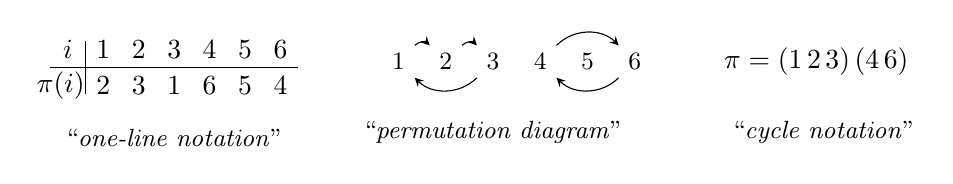
\begin{tikzpicture}[scale=.6,auto]
    \tikzstyle{n} = [inner sep=1pt]
    \tikzstyle{Left} = [draw,bend left=45,-stealth]
    \tikzstyle{Right} = [draw,bend right=45,-stealth]
    %%
    \begin{scope}[shift={(0,-.5)},scale=.75]
      \draw (-.5,.5) -- (6.5,.5); \draw (.5,-.25) -- (.5,1.25);
      \node at (0,1) {$i$}; \node at (-.2,0) {$\pi(i)$}; 
      \node at (1,1) {$1$}; \node at (1,0) {$2$};
      \node at (2,1) {$2$}; \node at (2,0) {$3$};
      \node at (3,1) {$3$}; \node at (3,0) {$1$};
      \node at (4,1) {$4$}; \node at (4,0) {$6$};
      \node at (5,1) {$5$}; \node at (5,0) {$5$};
      \node at (6,1) {$6$}; \node at (6,0) {$4$};
      \node at (3,-1.5) {\small ``\emph{one-line notation}''};
    \end{scope} 
    %%
    \begin{scope}[shift={(6,0)}]
      \tikzstyle{every node}=[font=\small]
      \node (1) at (1,0) {$1$};
      \node (2) at (2,0) {$2$};
      \node (3) at (3,0) {$3$};
      \node (4) at (4,0) {$4$};
      \node (5) at (5,0) {$5$};
      \node (6) at (6,0) {$6$};
      \path [Left] (1) to (2); \path [Left] (2) to (3); \path [Left] (3) to (1);
      \path [Left] (4) to (6); \path [Left] (6) to (4);
      \node at (3,-1.5) {\small``\emph{permutation diagram}''};
    \end{scope}
    %%
    \begin{scope}[shift={(18,0)}]
      \node [anchor=east] at (0,0) {$\pi=(1\,2\,3)\,(4\,6)$};
      \node at (-2,-1.5) {\small``\emph{cycle notation}''};
    \end{scope}
  \end{tikzpicture}
  \]
  
 \end{frame}
 
%%====================================================================

\begin{frame}{Permutation notations} \smallskip
  
  \textbf{One-line notation}:\quad $\pi=231654$,\qquad
  $\sigma=564123$ \medskip\Pause
  
  \begin{columns}[t]
    
    \begin{column}{.475\textwidth}
      \Balert{Pros}: \Pause
      \begin{itemize}
      \item concise \Pause
      \item nice visualization of rearrangement \Pause
      \end{itemize}
    \end{column}
    
    \begin{column}{.475\textwidth}
      \Alert{Cons}: \Pause
      \begin{itemize}
      \item bad for combining permutations \Pause
      \item not clear where elements get mapped \Pause
      \item hard to compute the inverse \Pause
      \end{itemize}
    \end{column}
    
  \end{columns}

  \vspace{1mm}\Pause
  
  
  \textbf{Permutation diagram}:\quad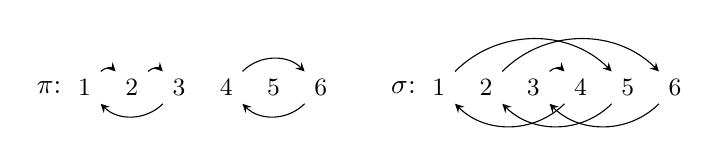
\begin{tikzpicture}[scale=.6,baseline=-.5ex]
  \tikzstyle{n} = [inner sep=1pt]
  \tikzstyle{Left} = [draw,bend left=45,-stealth]
  \tikzstyle{Right} = [draw,bend right=45,-stealth]
  %%
  \begin{scope}[shift={(0,0)}]
    \tikzstyle{every node}=[font=\small]
    %%
    \node at (.25,0) {\normalsize $\pi$:};
    \node (1) at (1,0) {$1$};
    \node (2) at (2,0) {$2$};
    \node (3) at (3,0) {$3$};
    \node (4) at (4,0) {$4$};
    \node (5) at (5,0) {$5$};
    \node (6) at (6,0) {$6$};
    \path [Left] (1) to (2); \path [Left] (2) to (3); \path [Left] (3) to (1);
    \path [Left] (4) to (6); \path [Left] (6) to (4);
  \end{scope}
  %%
  \begin{scope}[shift={(7.5,0)}]
    \tikzstyle{every node}=[font=\small]
    \node at (.25,0) {\normalsize $\sigma$:};
    \node (1) at (1,0) {$1$};
    \node (2) at (2,0) {$2$};
    \node (3) at (3,0) {$3$};
    \node (4) at (4,0) {$4$};
    \node (5) at (5,0) {$5$};
    \node (6) at (6,0) {$6$};
    \path [Left] (1) to (5); \path [Left] (5) to (2); \path [Left] (2) to (6);
    \path [Left] (6) to (3); \path [Left] (3) to (4); \path [Left] (4) to (1);
  \end{scope}
  \end{tikzpicture}
  
  \Pause
  
  \begin{columns}[t]    
    \begin{column}{.475\textwidth}
      \Balert{Pros}: \Pause
      \begin{itemize}
      \item can see where elements get mapped \Pause
      \item easy to compute inverses \Pause
      \item convenient for combining permutations \Pause
      \end{itemize}
    \end{column}
    %%
    \begin{column}{.475\textwidth}
      \Alert{Cons}: \Pause
      \begin{itemize}
      \item cumbersome to write \Pause
      \item can get tangled \Pause
      \end{itemize}
    \end{column}
  \end{columns}
  
  \vspace{4mm}%\Pause
  
  \textbf{Cycle notation}:\quad $\pi=(1\,2\,3)\,(4\,6)$,\qquad
  $\sigma=(1\,5\,2\,6\,3\,4)$; \medskip\Pause
  
  \begin{columns}[t]
    \begin{column}{.475\textwidth}
      \Balert{Pros}: \Pause
      \begin{itemize}
      \item short and concise \Pause
      \item easy to see the disjoint cycles \Pause
      \item convenient for combining permutations \Pause
      \end{itemize}
    \end{column}
    %%
    \begin{column}{.475\textwidth}
      \Alert{Cons}: \Pause
      \begin{itemize}
      \item representation isn't unique \Pause
      \item not clear what $n$ is
      \end{itemize}
    \end{column}
  \end{columns}
  
\end{frame}

%%====================================================================

\begin{frame}{Cycle notation} \smallskip
  
  The cycle $(1\,4\,6\,5)$ means
  \[
  \text{``\emph{1 goes to 4, which goes to 6, which does to 5, which goes
    back to 1}.''}
  \]
  \Pause Thus, we can write
  $(1\,4\,6\,5)=(4\,6\,5\,1)=(6\,5\,1\,4)=(5\,1\,4\,6)$. \medskip\Pause

  To find the \Balert{inverse} of a cycle, write it backwards:
  \[
  (1\,4\,6\,5)^{-1}=(5\,6\,4\,1)\Pause=(1\,5\,6\,4)=\cdots
  \]
  \Pause Though it's not necessary, we usually prefer to begin a cycle with
  its smallest number.
  
  \Pause
  
  \begin{exampleblock}{Remark}
    Every permutation in $S_n$ can be written in cycle notation as a
    product of \Balert{disjoint cycles}, and this is unique up to
    commuting and cyclically shifting cycles.
  \end{exampleblock}

  \Pause
  
  For example, consider the following permutation in $S_{10}$: \vspace{-1mm}
  \[
  \begin{tikzpicture}[scale=.55,auto,baseline=-1ex]
    \tikzstyle{n} = [inner sep=1pt]
    \tikzstyle{p} = [draw,bend left=45,-stealth]
    \tikzstyle{q} = [draw,bend left=35,-stealth]
    \tikzstyle{p-blue} = [draw,eBlue,bend left=45,-stealth]
    \tikzstyle{q-blue} = [draw,eBlue,bend left=35,-stealth]
    \tikzstyle{p-red} = [draw,eRed,bend left=45,-stealth]
    \tikzstyle{p-green} = [draw,eGreen,bend left=45,-stealth]
    \tikzstyle{every node}=[font=\scriptsize]
    %%
    \node [n] (1) at (1,0) {$1$};
    \node [n] (2) at (2,0) {$2$};
    \node [n] (3) at (3,0) {$3$};
    \node [n] (4) at (4,0) {$4$};
    \node [n] (5) at (5,0) {$5$};
    \node [n] (6) at (6,0) {$6$};
    \node [n] (7) at (7,0) {$7$};
    \node [n] (8) at (8,0) {$8$};
    \node [n] (9) at (9,0) {$9$};
    \node [n] (10) at (10,0) {$10$};
    \path [p-blue] (1) to (4);
    \path [p-blue] (4) to (6);
    \path [p-blue] (6) to (5);
    \path [q-blue] (5) to (1);
    \path [p-red] (2) to (3);
    \path [p-red] (3) to (2);
    \path [p-green] (8) to (10);
    \path [p-green] (10) to (9);
    \path [p-green] (9) to (8);
  \end{tikzpicture}
  \qquad \text{as} \qquad
  {\color{xBlue}(1\;4\;6\;5)}\,{\color{xRed}(2\;3)}
  \,{\color{xGreen}(8\;10\;9)}.
  \]
  This is a product of four disjoint cycles. \Pause Since they are
  disjoint, they commute:
  \[
    {\color{xBlue}(1465)}\,{\color{xRed}(23)}\,
    {\color{xGreen}(8\;10\;9)}
    ={\color{xRed}(23)}\,{\color{xGreen}(8\;10\;9)}\,
    {\color{xBlue}(1465)}
    ={\color{xRed}(23)}\,{\color{xGreen}(8\;10\;9)}\,
    {\color{xBlue}(1465)}=\cdots
  \]
    
\end{frame}

%%====================================================================

\begin{frame}{Composing permutations}

  \begin{exampleblock}{Remark}
    The \Balert{order} of a permutation is the least common multiple
    of the sizes of its disjoint cycles.
  \end{exampleblock}

  \smallskip\Pause

  For example, $(1\;3\;8\;6)(2\;9\;7\;4\;10\;5)\in S_{10}$ has order
  $12$; this should be intuitive. \medskip\Pause
  
  When cycles are not disjoint, order matters. \medskip\Pause

  Many books compose permutations from right-to-left, due to function
  composition. \medskip\Pause

  Since we have been using \Balert{right Cayley graphs}, we will
  compose them from left-to-right. \smallskip\Pause

  \begin{alertblock}{Notational convention}
    Composition of permutations will be done
    \Alert{left-to-right}. \Pause That is, given $\pi,\sigma\in S_n$,
    \[
    \pi\sigma\quad\text{means ``\emph{do $\pi$, then do $\sigma$}''}.
    \]
  \end{alertblock}

  \smallskip\Pause
  
  The main drawback about our convention is that it does not work well
  with function notation applied to elements, like $\pi(i)$.

  \medskip\Pause
  
  For example, notice that
  \[
  (\pi\sigma)(i)=\sigma(\pi(i))\neq\pi(\sigma(i)).
  \]
  \Pause However, we will hardly ever use this notation, so that
  drawback is minimal.
  
\end{frame}

%%====================================================================

\begin{frame}{Composing permutations} \smallskip
  
  Here are two ways illustrating how permutations are composed, with
  the example
  \[
  \begin{tikzpicture}[scale=.6,auto]
    %%
    \begin{scope}[shift={(0,-.5)},scale=.75]
      \node at (-2.5,.5) {\emph{First do}};
      \draw[xRed] (-.5,.5) -- (6.5,.5); \draw[xRed] (.5,-.25) -- (.5,1.25);
      \node[xRed] at (0,1) {$i$}; \node[xRed] at (-.2,0) {$\pi(i)$}; 
      \node[xRed] at (1,1) {$1$}; \node[xRed] at (1,0) {$4$};
      \node[xRed] at (2,1) {$2$}; \node[xRed] at (2,0) {$3$};
      \node[xRed] at (3,1) {$3$}; \node[xRed] at (3,0) {$1$};
      \node[xRed] at (4,1) {$4$}; \node[xRed] at (4,0) {$2$};
      \node[xRed] at (5,1) {$5$}; \node[xRed] at (5,0) {$6$};
      \node[xRed] at (6,1) {$6$}; \node[xRed] at (6,0) {$5$};
    \end{scope}
    %%
    \begin{scope}[shift={(9,-.5)},scale=.75]
      \node at (-3,.5) {\emph{then do}};
      \draw[xBlue] (-.5,.5) -- (6.5,.5); \draw[xBlue] (.5,-.25) -- (.5,1.25);
      \node[xBlue] at (0,1) {$i$}; \node[xBlue] at (-.2,0) {$\sigma(i)$}; 
      \node[xBlue] at (1,1) {$1$}; \node[xBlue] at (1,0) {$2$};
      \node[xBlue] at (2,1) {$2$}; \node[xBlue] at (2,0) {$1$};
      \node[xBlue] at (3,1) {$3$}; \node[xBlue] at (3,0) {$3$};
      \node[xBlue] at (4,1) {$4$}; \node[xBlue] at (4,0) {$6$};
      \node[xBlue] at (5,1) {$5$}; \node[xBlue] at (5,0) {$4$};
      \node[xBlue] at (6,1) {$6$}; \node[xBlue] at (6,0) {$5$};
    \end{scope}
  \end{tikzpicture}
  \]
  
  \vspace{-2mm}
  
  \begin{itemize}
  \item ``By stacking:''
    %% Red diagram stacked on a blue diagram = purple diagram
    \[
    \begin{tikzpicture}[scale=.8,auto,shorten >= -2pt,shorten <= -2pt]
      %%
      %% Red and blue permutation diagrams stacked
      %%
      \begin{scope}[shift={(0,0)},xscale=.6,yscale=1.5]
        \tikzstyle{every node}=[font=\small]
        %%
        \node (1) at (1,2) {$1$};
        \node (2) at (2,2) {$2$};
        \node (3) at (3,2) {$3$};
        \node (4) at (4,2) {$4$};
        \node (5) at (5,2) {$5$};
        \node (6) at (6,2) {$6$};
        \node (1m) at (1,1) {$1$};
        \node (2m) at (2,1) {$2$};
        \node (3m) at (3,1) {$3$};
        \node (4m) at (4,1) {$4$};
        \node (5m) at (5,1) {$5$};
        \node (6m) at (6,1) {$6$};
        \node (1b) at (1,0) {$1$};
        \node (2b) at (2,0) {$2$};
        \node (3b) at (3,0) {$3$};
        \node (4b) at (4,0) {$4$};
        \node (5b) at (5,0) {$5$};
        \node (6b) at (6,0) {$6$};
        \node[xRed] at (-1.8,1.5) {\normalsize \emph{first } $(1423)(56)$};
        \node[xBlue] at (-1.8,.5) {\normalsize \emph{then } $(12)(465)$};
        %%
        \draw [r] (1) to (4m); \draw [r] (4) to (2m); 
        \draw [r] (2) to (3m); \draw [r] (3) to (1m); 
        \draw [r] (5) to (6m); \draw [r] (6) to (5m);  
        %%
        \draw [b] (1m) to (2b); \draw [b] (2m) to (1b); 
        \draw [b] (4m) to (6b); \draw [b] (6m) to (5b); 
        \draw [b] (5m) to (4b); \draw [b] (3m) to (3b);  
        \node at (8.25,1) {\normalsize $=$};
      \end{scope}
      %%
      %% Purple permutation diagram
      %%
      \begin{scope}[shift={(5,0)},xscale=.6,,yscale=1.5]
        \tikzstyle{every node}=[font=\small]
        \node (1) at (1,2) {$1$};
        \node (2) at (2,2) {$2$};
        \node (3) at (3,2) {$3$};
        \node (4) at (4,2) {$4$};
        \node (5) at (5,2) {$5$};
        \node (6) at (6,2) {$6$};
        \node (1b) at (1,0) {$1$};
        \node (2b) at (2,0) {$2$};
        \node (3b) at (3,0) {$3$};
        \node (4b) at (4,0) {$4$};
        \node (5b) at (5,0) {$5$};
        \node (6b) at (6,0) {$6$};
        \node[xPurple] at (7.7,1) {\normalsize $(164)(23)$};
        \draw [p] (1) to (6b); \draw [p] (6) to (4b); 
        \draw [p] (4) to (1b); \draw [p] (2) to (3b); 
        \draw [p] (3) to (2b); \draw [p] (5) to (5b);  
      \end{scope}
    \end{tikzpicture}
    \]
    
  \item ``By cycles:''
    %%
    %% Permutation diagrams showing composition of permutations
    \[
    \begin{tikzpicture}[scale=.5,auto]
      \tikzstyle{n} = [inner sep=1pt]
      \tikzstyle{p-b} = [draw,bend left=45,-stealth,eBlue]
      \tikzstyle{p-r} = [draw,bend left=45,-stealth,eRed]
      \tikzstyle{p-p} = [draw,bend left=45,-stealth,ePurple]
      \tikzstyle{every node}=[font=\footnotesize]
      %%
      \begin{scope}[shift={(0,0)}]
        \node [n] (1) at (1,0) {$1$};
        \node [n] (2) at (2,0) {$2$};
        \node [n] (3) at (3,0) {$3$};
        \node [n] (4) at (4,0) {$4$};
        \node [n] (5) at (5,0) {$5$};
        \node [n] (6) at (6,0) {$6$};
        \path [p-r] (1) to (4); \path [p-r] (4) to (2);
        \path [p-r] (2) to (3); \path [p-r] (3) to (1);
        \path [p-r] (5) to (6); \path [p-r] (6) to (5);
        \node at (3.5,-1.5) {\small \Alert{\emph{first\; }$(1423)(56)$}};
        \node [n] at (7,0) {\Large$*$};
      \end{scope}
      %%
      \begin{scope}[shift={(7,0)}]
        \node [n] (1) at (1,0) {$1$};
        \node [n] (2) at (2,0) {$2$};
        \node [n] (3) at (3,0) {$3$};
        \node [n] (4) at (4,0) {$4$};
        \node [n] (5) at (5,0) {$5$};
        \node [n] (6) at (6,0) {$6$};
        \path [p-b] (1) to (2); \path [p-b] (2) to (1);
        \path [p-b] (4) to (6); \path [p-b] (6) to (5);
        \path [p-b] (5) to (4);
        \node at (3.5,-1.5) {\small \Balert{\emph{then\; }$(12)(465)$}};
        \node [n] at (7,0) {$=$};
      \end{scope}
      %%
      \begin{scope}[shift={(14,0)}]
        \node [n] (1) at (1,0) {$1$};
        \node [n] (2) at (2,0) {$2$};
        \node [n] (3) at (3,0) {$3$};
        \node [n] (4) at (4,0) {$4$};
        \node [n] (5) at (5,0) {$5$};
        \node [n] (6) at (6,0) {$6$};
        \path [p-p] (1) to (6); \path [p-p] (6) to (4);
        \path [p-p] (4) to (1);
        \path [p-p] (2) to (3); \path [p-p] (3) to (2);
        \node at (3.5,-1.5) {\small \Palert{$(164)(23)$}};
      \end{scope}
    \end{tikzpicture}
    \]
  \end{itemize}
  
\end{frame}

%%====================================================================

\begin{frame}{Composing permutations in cycle notation} %\Pause

  Let's practice composing two permutations: 

  \vspace{-1mm}

  %%
  %% Permutation diagrams showing composition of permutations  
  \[
  \begin{tikzpicture}[scale=.5,auto]
    \tikzstyle{n} = [inner sep=1pt]
    \tikzstyle{p-b} = [draw,bend left=45,-stealth,eBlue]
    \tikzstyle{p-r} = [draw,bend left=45,-stealth,eRed]
    \tikzstyle{p-p} = [draw,bend left=45,-stealth,ePurple]
    \tikzstyle{every node}=[font=\footnotesize]
    %%
    \begin{scope}[shift={(0,0)}]
      \node [n] (1) at (1,0) {$1$};
      \node [n] (2) at (2,0) {$2$};
      \node [n] (3) at (3,0) {$3$};
      \node [n] (4) at (4,0) {$4$};
      \node [n] (5) at (5,0) {$5$};
      \node [n] (6) at (6,0) {$6$};
      \path [p-r] (1) to (4); \path [p-r] (4) to (2);
      \path [p-r] (2) to (3); \path [p-r] (3) to (1);
      \path [p-r] (5) to (6); \path [p-r] (6) to (5);
      \node at (3.5,-1.5) {\small \Alert{\emph{first\; }$(1423)(56)$}};
      \node [n] at (7,0) {\Large$*$};
    \end{scope}
    %%
    \begin{scope}[shift={(7,0)}]
      \node [n] (1) at (1,0) {$1$};
      \node [n] (2) at (2,0) {$2$};
      \node [n] (3) at (3,0) {$3$};
      \node [n] (4) at (4,0) {$4$};
      \node [n] (5) at (5,0) {$5$};
      \node [n] (6) at (6,0) {$6$};
      \path [p-b] (1) to (2); \path [p-b] (2) to (1);
      \path [p-b] (4) to (6); \path [p-b] (6) to (5);
      \path [p-b] (5) to (4);
      \node at (3.5,-1.5) {\small \Balert{\emph{then }$(12)(465)$}};
      \node [n] at (7,0) {$=$};
    \end{scope}
    %%
    \begin{scope}[shift={(14,0)}]
      \node [n] (1) at (1,0) {$1$};
      \node [n] (2) at (2,0) {$2$};
      \node [n] (3) at (3,0) {$3$};
      \node [n] (4) at (4,0) {$4$};
      \node [n] (5) at (5,0) {$5$};
      \node [n] (6) at (6,0) {$6$};
      \path [p-p] (1) to (6); \path [p-p] (6) to (4);
      \path [p-p] (4) to (1);
      \path [p-p] (2) to (3); \path [p-p] (3) to (2);
      \node at (3.5,-1.5) {\small \Palert{$(164)(23)$}};
    \end{scope}
  \end{tikzpicture}
  \]
  
  \Pause Let's now do that in slow motion. \medskip\Pause
  
  In the example above, we start with $1$ and then read off: \smallskip\Pause
  
  \begin{itemize} 
  \item ``\Alert{\textbf{1} goes to 4}, then \Balert{4 goes to 6}'';
    \qquad\Pause Write: $\Palert{(1\;6}$ \smallskip\Pause 
  \item ``\Alert{6 goes to 5}, then \Balert{5 goes to 4}''; \qquad\Pause Write:
    $\Palert{(1\;6\;4}$ \smallskip\Pause
  \item ``\Alert{4 goes to 2}, then \Balert{2 goes to \textbf{1}}'';
    \qquad\Pause Write: $\Palert{(1\;6\;4)}$, and start a new
    cycle. \smallskip\Pause
  \item ``\Alert{\textbf{2} goes to 3}, then \Balert{3 is fixed}'';
    \qquad\hspace{3.25mm}\Pause Write:
    $\Palert{(1\;6\;4)\;(2\;3}$ \smallskip\Pause
  \item ``\Alert{3 goes to 1}, then \Balert{1 goes to \textbf{2}}'';
    \qquad\Pause Write: $\Palert{(1\;6\;4)\;(2\;3)}$, and start a new
    cycle. \smallskip\Pause
  \item ``\Alert{\textbf{5} goes to 6}, then \Balert{6 goes to \textbf{5}}'';
    \qquad\Pause Write: $\Palert{(1\;6\;4)\;(2\;3)\;(5)}$; now we're done.
  \end{itemize}

  \medskip\Pause
  
  We typically omit $1$-cycles (fixed points), so the permutation
  above is just $\Palert{(1\;6\;4)\;(2\;3)}$.

\end{frame}

%%====================================================================
%%====================================================================

\begin{frame}{Cayley's theorem}


  A set of permutations that forms a group is called a
  \Alert{permutation group}. \bigskip\Pause

  A fundamental theorem by British mathematician Arthur Cayley
  (1821--1895) says that every finite group can be thought of as a
  collection of permutations. \bigskip\Pause

  This is clear for groups of symmetries like $V_4$, $C_n$, or
  $D_n$, but less so for groups like $Q_8$. \medskip\Pause

  \begin{block}{Cayley's theorem}
    Every finite group is ``isomorphic to'' a collection of permutations,
    i.e., some subgroup of $S_n$.
  \end{block}

  \medskip\Pause
  
  We don't have the mathematical tools to prove this formally, but
  %\medskip\Pause
  we'll get a $1$-line proof when we study group actions.  \bigskip\Pause

  Let's make an intuitive argument, though.
  
\end{frame}

%%====================================================================

\begin{frame}{Constructing permutations from a Cayley graph} %\Pause
  
  Here is an algorithm given a {\color{xRed}Cayley graph} with $n$
  nodes: \smallskip
  
  \Pause
  
  \begin{enumerate}
  \item number the nodes $1$ through $n$, \smallskip\Pause
  \item interpret each arrow type in the Cayley graph as a permutation.
  \end{enumerate} 
  
  \medskip\Pause

  Take the permutations corresponding to the generators. 
  
  \medskip\Pause 
  
  \begin{exampleblock}{Example}
    
    Let's try this with $D_3=\<{\color{xRed}r},{\color{xBlue}f}\>$.
    
    
    %% Cayley graph of D_3 w/ permutation diagrams, illustrating Cayley's thm
    \[
    \begin{tikzpicture}
      \tikzstyle{v} = [circle, draw, fill=lightgray,inner sep=0pt, 
        minimum size=3.5mm]
      \tikzstyle{n} = [inner sep=1pt]
      \tikzstyle{P} = [draw,bend left=45,-stealth]
      %%
      %% Cayley graph of D3 with nodes labeled 1,...,6
      %%
      \begin{scope}[scale=.65,auto]
        \tikzstyle{every node}=[font=\small]
        \node (1) at (0:2) [v] {$1$};
        \node (r) at (120:2) [v] {$2$};
        \node (r2) at (240:2) [v] {$3$};
        \node (f) at (0:1) [v] {$4$};
        \node (rf) at (120:1) [v] {$5$};
        \node (r2f) at (240:1) [v] {$6$};
        \draw [r] (1) to [bend right=35] (r);
        \draw [r] (r) to [bend right=35] (r2);
        \draw [r] (r2) to [bend right=35] (1);
        \draw [r] (f) to [bend left=30] (r2f);
        \draw [r] (r2f) to [bend left=30] (rf);
        \draw [r] (rf) to [bend left=30] (f);
        \draw [bb] (1) to (f);
        \draw [bb] (r) to (rf);
        \draw [bb] (r2) to (r2f);
      \end{scope}
      %%
      %% Two permutation diagrams.
      %%
      \begin{scope}[scale=.6,shift={(4,1)}]
      \node [n] (r1) at (1,0) {$1$};
      \node [n] (r2) at (2,0) {$2$};
      \node [n] (r3) at (3,0) {$3$};
      \node [n] (r4) at (4,0) {$4$};
      \node [n] (r5) at (5,0) {$5$};
      \node [n] (r6) at (6,0) {$6$};
      \path [P,eRed] (r1) to (r2);
      \path [P,eRed] (r2) to (r3);
      \path [P,eRed] (r3) to (r1);
      \path [P,eRed] (r4) to (r6);
      \path [P,eRed] (r6) to (r5);
      \path [P,eRed] (r5) to (r4);
      \end{scope}
      %%
    \begin{scope}[scale=.6,shift={(4,-1)}]
      \node [n] (b1) at (1,0) {$1$};
      \node [n] (b2) at (2,0) {$2$};
      \node [n] (b3) at (3,0) {$3$};
      \node [n] (b4) at (4,0) {$4$};
      \node [n] (b5) at (5,0) {$5$};
      \node [n] (b6) at (6,0) {$6$};
      \path [P,eBlue] (b1) to (b4);
      \path [P,eBlue] (b2) to (b5);
      \path [P,eBlue] (b3) to (b6);
      \path [P,eBlue] (b4) to (b1);
      \path [P,eBlue] (b5) to (b2);
      \path [P,eBlue] (b6) to (b3);
      \end{scope}
    \end{tikzpicture}
  \]

  \Pause
  
  We see that $D_3$ is isomorphic to the subgroup 
  $\big\<{\color{xRed}(123)(456)},\;{\color{xBlue}(14)(25)(36)}\big\>$ of $S_6$.
  \end{exampleblock}

  \begin{alertblock}{Question:}
    Would this have worked if we had chosen a different numbering?
  \end{alertblock}
  
\end{frame}

%%====================================================================

\begin{frame}{Constructing permutations from a Cayley table} %\Pause
  
  Here is an algorithm given a {\color{xBlue}Cayley table} with
  $n$ elements:
  
  \Pause

  \begin{enumerate}
  \item replace the table headings with $1$ through $n$, \Pause
  \item make the appropriate replacements throughout the rest of the
    table, \Pause
  \item interpret each row (or column) as a permutation. 
  \end{enumerate}
  
 \Pause

  Take the permutations corresponding to \emph{any} generating set. 

  %\smallskip\Pause

  \begin{exampleblock}{Example}
    
  Let's try this with the Cayley table for
  $D_3=\<{\color{xRed}r},{\color{xBlue}f}\>$.

  %% Cayley table of D_3 numbered 1,...,6, and permutations defined by rows
  \[
  \begin{tikzpicture}[scale=.53,box/.style={anchor=center}]
    \colorlet{color-e}{tYellow}
    \colorlet{color-r}{tRed}
    \colorlet{color-r2}{tOrange}
    \colorlet{color-f}{tBlue}
    \colorlet{color-rf}{tGreen}
    \colorlet{color-r2f}{tPurple}
    \newcommand*{\n}{7}%
    %%
    %% Cayley table of D_3 numbered 1,...,6
    %%
    \begin{scope}[shift={(0,0)}]
      \path[fill=color-e] (-.1,6) rectangle ++(1,1);
      \path[fill=color-r] (-.1,5) rectangle ++(1,1);
      \path[fill=color-r2] (-.1,4) rectangle ++(1,1);
      \path[fill=color-f] (-.1,3) rectangle ++(1,1);
      \path[fill=color-rf] (-.1,2) rectangle ++(1,1);
      \path[fill=color-r2f] (-.1,1) rectangle ++(1,1);
      %%
      \path[fill=color-e] (1,7.1) rectangle ++(1,1);
      \path[fill=color-r] (2,7.1) rectangle ++(1,1);
      \path[fill=color-r2] (3,7.1) rectangle ++(1,1);
      \path[fill=color-f] (4,7.1) rectangle ++(1,1);
      \path[fill=color-rf] (5,7.1) rectangle ++(1,1);
      \path[fill=color-r2f] (6,7.1) rectangle ++(1,1);
      %%
      \path[fill=color-e] (1,6) rectangle ++(1,1);
      \path[fill=color-r] (1,5) rectangle ++(1,1);
      \path[fill=color-r2] (1,4) rectangle ++(1,1);
      \path[fill=color-f] (1,3) rectangle ++(1,1);
      \path[fill=color-rf] (1,2) rectangle ++(1,1);
      \path[fill=color-r2f] (1,1) rectangle ++(1,1);
      %%
      \path[fill=color-r] (2,6) rectangle ++(1,1);
      \path[fill=color-r2] (2,5) rectangle ++(1,1);
      \path[fill=color-e] (2,4) rectangle ++(1,1);
      \path[fill=color-r2f] (2,3) rectangle ++(1,1);
      \path[fill=color-f] (2,2) rectangle ++(1,1);
      \path[fill=color-rf] (2,1) rectangle ++(1,1);
      %%
      \path[fill=color-r2] (3,6) rectangle ++(1,1);
      \path[fill=color-e] (3,5) rectangle ++(1,1);
      \path[fill=color-r] (3,4) rectangle ++(1,1);
      \path[fill=color-rf] (3,3) rectangle ++(1,1);
      \path[fill=color-r2f] (3,2) rectangle ++(1,1);
      \path[fill=color-f] (3,1) rectangle ++(1,1);
      %%
      \path[fill=color-f] (4,6) rectangle ++(1,1);
      \path[fill=color-rf] (4,5) rectangle ++(1,1);
      \path[fill=color-r2f] (4,4) rectangle ++(1,1);
      \path[fill=color-e] (4,3) rectangle ++(1,1);
      \path[fill=color-r] (4,2) rectangle ++(1,1);
      \path[fill=color-r2] (4,1) rectangle ++(1,1);
      %%
      \path[fill=color-rf] (5,6) rectangle ++(1,1);
      \path[fill=color-r2f] (5,5) rectangle ++(1,1);
      \path[fill=color-f] (5,4) rectangle ++(1,1);
      \path[fill=color-r2] (5,3) rectangle ++(1,1);
      \path[fill=color-e] (5,2) rectangle ++(1,1);
      \path[fill=color-r] (5,1) rectangle ++(1,1);
      %%
      \path[fill=color-r2f] (6,6) rectangle ++(1,1);
      \path[fill=color-f] (6,5) rectangle ++(1,1);
      \path[fill=color-rf] (6,4) rectangle ++(1,1);
      \path[fill=color-r] (6,3) rectangle ++(1,1);
      \path[fill=color-r2] (6,2) rectangle ++(1,1);
      \path[fill=color-e] (6,1) rectangle ++(1,1);
      %%
      \foreach \i in {1,...,\n} {
        \draw [very thin] (\i,1) -- (\i,\n); 
        \draw [very thin] (\i,\n+.1) -- (\i,\n+1.1); 
        \draw [very thin] (1,\i) -- (\n,\i); 
        \draw [very thin] (-.1,\i) -- (.9,\i); 
      } 
      \draw [very thin] (1,\n+.1) rectangle (\n,\n+1.1);
      \draw [very thin] (-.1,1) rectangle (.9,\n);
      \node [box] at (0.4,6.5) {$1$};
      \node [box] at (0.4,5.5) {$2$};
      \node [box] at (0.4,4.5) {$3$};
      \node [box] at (0.4,3.5) {$4$};
      \node [box] at (0.4,2.5) {$5$};
      \node [box] at (0.4,1.5) {$6$};
      %%
      \node [box] at (1.5,7.6) {$1$};
      \node [box] at (2.5,7.6) {$2$};
      \node [box] at (3.5,7.6) {$3$};
      \node [box] at (4.5,7.6) {$4$};
      \node [box] at (5.5,7.6) {$5$};
      \node [box] at (6.5,7.6) {$6$}; %
      %%
      \node [box] at (1.5,6.5) {$1$};
      \node [box] at (1.5,5.5) {$2$};
      \node [box] at (1.5,4.5) {$3$};
      \node [box] at (1.5,3.5) {$4$};
      \node [box] at (1.5,2.5) {$5$};
      \node [box] at (1.5,1.5) {$6$};
      %%
      \node [box] at (2.5,6.5) {$2$};
      \node [box] at (2.5,5.5) {$3$};
      \node [box] at (2.5,4.5) {$1$};
      \node [box] at (2.5,3.5) {$6$};
      \node [box] at (2.5,2.5) {$4$};
      \node [box] at (2.5,1.5) {$5$};
      %%
      \node [box] at (3.5,6.5) {$3$};
      \node [box] at (3.5,5.5) {$1$};
      \node [box] at (3.5,4.5) {$2$};
      \node [box] at (3.5,3.5) {$5$};
      \node [box] at (3.5,2.5) {$6$};
      \node [box] at (3.5,1.5) {$4$};
      %%
      \node [box] at (4.5,6.5) {$4$};
      \node [box] at (4.5,5.5) {$5$};
      \node [box] at (4.5,4.5) {$6$};
      \node [box] at (4.5,3.5) {$1$};
      \node [box] at (4.5,2.5) {$2$};
      \node [box] at (4.5,1.5) {$3$};
      %%
      \node [box] at (5.5,6.5) {$5$};
      \node [box] at (5.5,5.5) {$6$};
      \node [box] at (5.5,4.5) {$4$};
      \node [box] at (5.5,3.5) {$3$};
      \node [box] at (5.5,2.5) {$1$};
      \node [box] at (5.5,1.5) {$2$};
      %%
      \node [box] at (6.5,6.5) {$6$};
      \node [box] at (6.5,5.5) {$4$};
      \node [box] at (6.5,4.5) {$5$};
      \node [box] at (6.5,3.5) {$2$};
      \node [box] at (6.5,2.5) {$3$};
      \node [box] at (6.5,1.5) {$1$};
    \end{scope}
    %%
    %% Permutation diagrams for each row
    %%
    \begin{scope}[shift={(10,0)}]
      \tikzstyle{every node}=[font=\small]
      \tikzstyle{n} = [inner sep=1pt]
      \tikzstyle{P} = [draw,bend left=25,-stealth]
      %%
      \node[anchor=west] at (-1.5,6.5) {\textbf{Row 1} (1):};
      \node [n] (11) at (2,6.5) {$1$};
      \node [n] (12) at (3,6.5) {$2$};
      \node [n] (13) at (4,6.5) {$3$};
      \node [n] (14) at (5,6.5) {$4$};
      \node [n] (15) at (6,6.5) {$5$};
      \node [n] (16) at (7,6.5) {$6$};
      %%
      \node[anchor=west] at (-1.5,5.5) {\textbf{Row 2} ($r$):};
      \node [n] (21) at (2,5.5) {$1$};
      \node [n] (22) at (3,5.5) {$2$};
      \node [n] (23) at (4,5.5) {$3$};
      \node [n] (24) at (5,5.5) {$4$};
      \node [n] (25) at (6,5.5) {$5$};
      \node [n] (26) at (7,5.5) {$6$};
      \path [P,eRed] (21) to (22);
      \path [P,eRed] (22) to (23);
      \path [P,eRed] (23) to (21);
      \path [P,eRed] (24) to (25);
      \path [P,eRed] (25) to (26);
      \path [P,eRed] (26) to (24);
      %%
      \node[anchor=west] at (-1.5,4.5) {\textbf{Row 3} ($r^2$):};
      \node [n] (31) at (2,4.5) {$1$};
      \node [n] (32) at (3,4.5) {$2$};
      \node [n] (33) at (4,4.5) {$3$};
      \node [n] (34) at (5,4.5) {$4$};
      \node [n] (35) at (6,4.5) {$5$};
      \node [n] (36) at (7,4.5) {$6$};
      \path [P,eOrange] (31) to (33);
      \path [P,eOrange] (33) to (32);
      \path [P,eOrange] (32) to (31);
      \path [P,eOrange] (34) to (36);
      \path [P,eOrange] (36) to (35);
      \path [P,eOrange] (35) to (34);
      %%
      \tikzstyle{P} = [draw,bend left=20,-stealth]
       %% 
      \node[anchor=west] at (-1.5,3.5) {\textbf{Row 4} ($f$):};
      \node [n] (41) at (2,3.5) {$1$};
      \node [n] (42) at (3,3.5) {$2$};
      \node [n] (43) at (4,3.5) {$3$};
      \node [n] (44) at (5,3.5) {$4$};
      \node [n] (45) at (6,3.5) {$5$};
      \node [n] (46) at (7,3.5) {$6$};
      \path [P,eBlue] (41) to (44);
      \path [P,eBlue] (42) to (46);
      \path [P,eBlue] (43) to (45);
      \path [P,eBlue] (44) to (41);
      \path [P,eBlue] (45) to (43);
      \path [P,eBlue] (46) to (42);
      %%
      \node[anchor=west] at (-1.5,2.5) {\textbf{Row 5} ($rf$):};
      \node [n] (51) at (2,2.5) {$1$};
      \node [n] (52) at (3,2.5) {$2$};
      \node [n] (53) at (4,2.5) {$3$};
      \node [n] (54) at (5,2.5) {$4$};
      \node [n] (55) at (6,2.5) {$5$};
      \node [n] (56) at (7,2.5) {$6$};
      \path [P,eGreen] (51) to (55);
      \path [P,eGreen] (52) to (54);
      \path [P,eGreen] (53) to (56);
      \path [P,eGreen] (54) to (52);
      \path [P,eGreen] (55) to (51);
      \path [P,eGreen] (56) to (53);
      %%  
      \tikzstyle{P} = [draw,bend left=16,-stealth]
      %%
      \node[anchor=west] at (-1.5,1.5) {\textbf{Row 6} ($r^2\!f$):};
      \node [n] (61) at (2,1.5) {$1$};
      \node [n] (62) at (3,1.5) {$2$};
      \node [n] (63) at (4,1.5) {$3$};
      \node [n] (64) at (5,1.5) {$4$};
      \node [n] (65) at (6,1.5) {$5$};
      \node [n] (66) at (7,1.5) {$6$};
      \path [P,ePurple] (61) to (66);
      \path [P,ePurple] (62) to (65);
      \path [P,ePurple] (63) to (64);
      \path [P,ePurple] (64) to (63);
      \path [P,ePurple] (65) to (62);
      \path [P,ePurple] (66) to (61);      %%  
    \end{scope}
  \end{tikzpicture}
  \]
  
  \vspace{-2mm}\Pause

  We see that $D_3$ is isomorphic to the subgroup
  $\big\<\Alert{(123)(456)},\Balert{(14)(26)(35)}\big\>$ of $S_6$.
  \end{exampleblock}

\end{frame}

%%====================================================================


%Dihedral groups via reflections only
% NO PAUSES
\begin{frame}{Constructing permutations from a \alert{different} Cayley diagram}
  
  \begin{columns}
    \column{0.6 \textwidth}
      Another canonical way to generate $D_n$ is with \\ \alert{two reflections}:
      \begin{itemize}
      \item \Balert{$s:=f$}
      \item \Galert{$t:=fr=r^{n-1}f$} -- a different reflection!
      \end{itemize}
    \column{0.4\textwidth}
      \begin{tikzpicture}
        \colorlet{color1}{actBlue}
        \colorlet{color2}{actGreen}
        \colorlet{color3}{cosetPurple}
        \draw[dashed,thick,eBlue] (.5,1.5) to (.5,-.8);
        \draw[dashed,thick,ePurple] (-.5,-.307) to (1.5,.921);
        \draw[dashed,thick,eGreen] (-.5,.921) to (1.5,-.307);
        \draw[color1,fill=color1]
        (.5,.307)--(.25,.433)--(.5,.866)--(.75,.433)--cycle;
        \draw[color2,fill=color2] (.5,.307)--(.75,.433)--(1,0)--(.5,0)--cycle;
        \draw[color3,fill=color3] (.5,.307)--(.25,.433)--(0,0)--(.5,0)--cycle;
        \draw [black] (0,0)--(.5,.866)--(1,0)--cycle;
        \draw (.5,.55) node {$\mathbf{1}$}; 
        \draw (.3,.2) node {$\mathbf{2}$};\draw (.7,.2) node {$\mathbf{3}$};
        \node at (.5,1.75) {\color{xBlue}$s=f$};
        \node at (-.8,1.25) {\color{xGreen}$t=fr$};
        \draw[-stealth',eRed] (1.5,-.5) to[very thick,bend right=60] (1.7,.2);
        \node at (2,-.7) {\color{xRed}$st=r$};
      \end{tikzpicture}
  \end{columns}
   Composing these in either order is a rotation of $2\pi/n$ radians:
  \[
  st=f(fr)=r,\qquad ts=(fr)f=(r^{n-1}f)f=r^{n-1}.
  \]
  A group presentation with these generators is
  \[
  D_n=\big\<s,t\mid s^2=1,\;t^2=1,\;(st)^n=1\big\> 
  =\big\{\underbrace{1,st,ts,(st)^2,(ts)^2,\ldots,}_{\text{rotations}}\;
  \underbrace{s,t,sts,tst,\ldots}_{\text{reflections}}\big\}.
  \]
  
  % 2 Cayley graphs of D_3 = <r, f> = <s,t>, and the triangle
  \[
  \begin{tikzpicture}[scale=.6,auto]
    \colorlet{color1}{actBlue}
    \colorlet{color2}{actGreen}
    \colorlet{color3}{cosetPurple}
    \tikzstyle{P} = [draw,bend left=45,-stealth]
    \tikzstyle{n} = [inner sep=1pt]
    %%
    %% Cayley graph of D3
    %%
    \begin{scope}[shift={(0,0)},scale=.9]
      \tikzstyle{every node}=[font=\small]
      \tikzstyle{r-in} = [draw, very thick, eRed,-stealth,bend left=35]
      \tikzstyle{r-out} = [draw, very thick, eRed,-stealth,bend right=48]
      \node (e) at (0:2.4) [v] {$1$};
      \node (r) at (120:2.4) [v] {$r$};
      \node (r2) at (240:2.4) [v] {$r^2$};
      \node (f) at (0:1) [v] {$f$};
      \node (r2f) at (240:1) [v] {$r^2\!f$};
      \node (rf) at (120:1) [v] {$rf$};
      \draw [r-out] (e) to  (r);
      \draw [r-out] (r) to (r2);
      \draw [r-out] (r2) to (e);
      \draw [r-in] (f) to (r2f);
      \draw [r-in] (r2f) to (rf);
      \draw [r-in] (rf) to (f);
      \draw [bb] (e) to (f);
      \draw [bb] (r) to (rf);
      \draw [bb] (r2) to (r2f);
    \end{scope}
    %%
    %% Cayley graph of D4
    %%
    \begin{scope}[shift={(7,0)}]
      \tikzstyle{every node}=[font=\small]
      \node (e) at (90:2) [v] {$1$};
      \node (t) at (30:2) [v] {$t$};
      \node (ts) at (-30:2) [v] {$ts$};
      \node (sts) at (-90:2) [v] {$sts$};
      \node (st) at (-150:2) [v] {$st$};
      \node (s) at (150:2) [v] {$s$};
      \path[gg] (e) to (t);
      \path[bb] (t) to (ts);
      \path[gg] (ts) to (sts);
      \path[bb] (st) to (sts);
      \path[gg] (s) to (st);
      \path[bb] (e) to (s);
    \end{scope}
    %%%%
      %% Two permutation diagrams.
      %%
    \begin{scope}[shift={(10,1)}]
      \node [n] (r1) at (1,0) {$1$};
      \node [n] (r2) at (2,0) {$2$};
      \node [n] (r3) at (3,0) {$3$};
      \node [n] (r4) at (4,0) {$4$};
      \node [n] (r5) at (5,0) {$5$};
      \node [n] (r6) at (6,0) {$6$};
    \end{scope}
    %%
    \begin{scope}[shift={(10,-1)}]
      \node [n] (b1) at (1,0) {$1$};
      \node [n] (b2) at (2,0) {$2$};
      \node [n] (b3) at (3,0) {$3$};
      \node [n] (b4) at (4,0) {$4$};
      \node [n] (b5) at (5,0) {$5$};
      \node [n] (b6) at (6,0) {$6$};
    \end{scope}
  \end{tikzpicture}
  \]
  
\end{frame}

%%====================================================================


\begin{frame}{Transpositions} %\Pause
  
  A \alert{transposition} is a permutation that swaps two objects and
  fixes the rest, e.g.:
  
  \vspace{-1mm}

  %% Permutation diagram of (ij) in S_n
  \[
  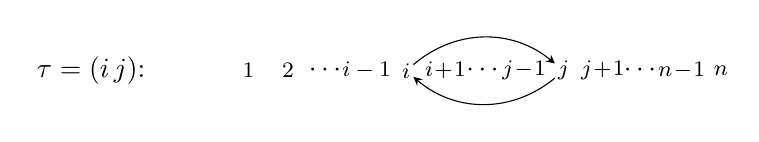
\begin{tikzpicture}[scale=.5,auto]
    \tikzstyle{n} = [inner sep=1pt]
    \tikzstyle{r} = [draw,bend left=40,-stealth]
    \tikzstyle{l} = [draw,bend left=40,-stealth]
    \tikzstyle{every node}=[font=\footnotesize]
    \node at (-3,0) {\normalsize $\tau=(i\,j)$:};
    \node [n] (1) at (1,0) {$1$};
    \node [n] (2) at (2,0) {$2$};
    \node [n] (3) at (3,0) {\normalsize $\cdots$};
    \node [n] (4) at (4,0) {$i-1$};
    \node [n] (5) at (5,0) {$i$};
    \node [n] (6) at (6,0) {$i\!+\!1$};
    \node [n] (7) at (7,0) {\normalsize $\cdots$};
    \node [n] (8) at (8,0) {$j\!-\!1$};
    \node [n] (9) at (9,0) {$j$};
    \node [n] (10) at (10,0) {$j\!+\!1$};
    \node [n] (11) at (11,0) {\normalsize $\cdots$};
    \node [n] (12) at (12,0) {$n\!-\!1$};
    \node [n] (13) at (13,0) {$n$};
    \path [r] (5) to (9);
    \path [l] (9) to (5);
  \end{tikzpicture}
  \]
  
  \vspace{-1mm}\Pause
  
  An \Balert{adjacent transposition} is one of the form $(i\;\;i\!+\!1)$. 

  \medskip\Pause

  \begin{alertblock}{Remark}
    There are three canonical types of generating sets for
    $S_n$: \smallskip\Pause
    \begin{itemize}
    \item A \Galert{transposition} and an \Alert{$n$-cycle},
      e.g.,: \vspace{-1mm}
      \[
      S_n=\big\<\,\Galert{(1\;2)},\;\;\Alert{(1\;2\,\cdots\,
        n\!-\!1\;\;n)}\big\>\,.
      \]

      \vspace{-2mm}
      
    \item \Balert{Adjacent transpositions}: \vspace{-2mm}
      \[
      S_n=\big\<\,(1\;2),\;(2\; 3),\;\dots,\; (n-1\;\;n)\big\>\,. 
      \]

      \vspace{-2mm}
      
    \item \Palert{Overlapping transpositions}: \vspace{-2mm}
      \[
      S_n=\big\<\,(1\;2),\;(1\; 3),\;\dots,\; (1\;\;n)\big\>\,. 
      \] \vspace{-4mm}\Pause
    \end{itemize}
  \end{alertblock}

  \begin{exampleblock}{Homework}
    Explain why each of these will generate the full $S_n$. \\ (It may be helpful to think about $n$ objects arranged in a row.)
  \end{exampleblock}
  
\end{frame}

%%====================================================================

\begin{frame}{Even and odd permutations} %\Pause
  
  \begin{exampleblock}{Remark}
    Every permutation in $S_n$ can be written as a product of transpositions... \alert{uniquely?}
  \end{exampleblock}
  
  \medskip\Pause

  \begin{itemize}
    \item Example: $(1\; 3\; 2) = (1\; 2) (2\; 3)$ \Pause
    \item Write $(1\; 3\; 5)$ as a product of transpositions. \Pause
    \item Write $(1\; 3\; 5)$ using only \Balert{adjacent transpositions}.
    \item Write $(1\; 3\; 5)$ using only \Palert{overlapping transpositions}.
  \end{itemize}
  
  \medskip\Pause
  
  \begin{block}{Proposition}
    The \alert{parity} of the number of transpositions of a fixed
    permutation is unique.
  \end{block}
  
  \Pause

  \begin{definition}
    An \Alert{even permutation} in $S_n$ can be written with an even
    number of transpositions. \\
    An \Balert{odd permutation} requires an odd number.
  \end{definition}

  \Pause
  
  \begin{exampleblock}{Remark}
    \begin{itemize}
    \item The product of two \Alert{even} permutations is \Alert{even}. (Why?) \Pause
    \item The product of two \Balert{odd} permutations is \Pause
    \item The product of an \Alert{even} and an \Balert{odd} permutation is 
    \end{itemize}
  \end{exampleblock}


\end{frame}

%%====================================================================

\begin{frame}{The alternating groups} \smallskip

  \begin{block}{Definition}
    The set of \Alert{even} permutations in $S_n$ is the \Alert{alternating
      group}, denoted $A_n$.
  \end{block}

  \Pause
  
  \begin{block}{Proposition}
    Exactly half of the permutations in $S_n$ are even, and so 
    $\displaystyle |A_n|=\tfrac{n!}{2}$.
  \end{block}

  \smallskip\Pause
  
  Rather than prove this using (messy) elementary methods now, we'll
  wait until we see the \Balert{isomorphism theorems} to get a 1-line
  proof. \medskip\Pause
  
  Here are Cayley graphs for $A_4$ on a \Balert{truncated tetrahedron} and
  \Galert{cuboctahedron}.
  
  %% Cayley graphs for A_4 on truncated tetrahedron and a cuboctahedron.
  \[
  \begin{tikzpicture}[scale=.6]
    %%
    %% A_4 Cayley graph on a truncated tetrahedron
    %% 
    \begin{scope}[shift={(0,0)},scale=1.95]
      \tikzstyle{v} = [circle, draw, fill=lightgray,inner sep=0pt,
        minimum size=3.5mm] 
      \tikzstyle{v-f} = [circle, draw, gray, fill=lightgray,inner sep=0pt,
        minimum size=3.5mm]
      \tikzstyle{every node}=[font=\tiny]
      %%
      \node (l1) at (-.05,.8) [v] {$x$};
      \node (l2) at (0,.4) [v] {$b$};
      \node (l3) at (.5,0) [v] {$c^2$};
      \node (t1) at (.85,2.5) [v] {$e$};
      \node (t2) at (1.3,2.8) [v] {$a^2$};
      \node (t3) at (1.8,2.55) [v] {$a$};
      \node (r1) at (2.4,.2) [v] {$d^2$};
      \node (r2) at (2.5,.7) [v-f] {\color{darkgray} $z$};
      \node (r3) at (2.9,.9) [v] {$c$};
      \node (m2) at (1.15,1.9) [v-f] {\color{darkgray} $b^2$};
      \node (m1) at (.8,1.25) [v-f] {\color{darkgray} $d$};
      \node (m3) at (1.5,1.3) [v-f] {\color{darkgray} $y$};
      \draw [rFaded] (r1) to (r2);
      \draw [rFaded] (r2) to (r3);
      \draw [bbFaded] (l2) to (m1);
      \draw [bbFaded] (m2) to (t2);
      \draw [bbFaded] (r2) to (m3);
      \draw [rFaded] (m1) to (m2);
      \draw [rFaded] (m2) to (m3);
      \draw [rFaded] (m3) to (m1);
      \draw [bb] (l1) to (t1);
      \draw [bb] (l3) to (r1);
      \draw [bb] (r3) to (t3);
      \draw [r] (l1) to (l2);
      \draw [r] (l2) to (l3);
      \draw [r] (l3) to (l1);
      \draw [r] (t1) to (t3);
      \draw [r] (t2) to (t1);
      \draw [r] (t3) to (t2);
      \draw [r] (r3) to (r1);
      \node at (0,-.2) {};
    \end{scope}
    %%
    %% A_4 Cayley graph on a cuboctahedron
    %%
    \begin{scope}[shift={(12,2.75)},scale=.95]
      \tikzstyle{v} = [circle, draw, fill=lightgray,inner sep=0pt,
        minimum size=1.75mm]
      %%
      \node (a2) at (45:1) [v] {};
      \node (a4) at (135:1) [v] {}; %{$\tiny *$};
      \node (a6) at (225:1) [v] {};
      \node (a8) at (315:1) [v] {};
      \node (b1) at (0:2) [v] {};
      \node (b3) at (90:2) [v] {};
      \node (b5) at (180:2) [v] {};
      \node (b7) at (270:2) [v] {};
      \node (c2) at (45:4) [v] {};
      \node (c4) at (135:4) [v] {};
      \node (c6) at (225:4) [v] {};
      \node (c8) at (315:4) [v] {};
      \draw [p] (b1) to (a8); \draw [p] (a8) to (a2); \draw [p] (a2) to (b1);
      \draw [p] (a4) to (a6); \draw [p] (a6) to (b5); \draw [p] (b5) to (a4);
      \draw [p] (c2) to (b3); \draw [p] (b3) to (c4); \draw [p] (c4) to (c2);
      \draw [p] (c6) to (b7); \draw [p] (b7) to (c8); \draw [p] (c8) to (c6);
      \draw [g] (b1) to (c2); \draw [g] (c2) to (c8); \draw [g] (c8) to (b1);
      \draw [g] (b5) to (c6); \draw [g] (c6) to (c4); \draw [g] (c4) to (b5);
      \draw [g] (b3) to (a2); \draw [g] (a2) to (a4); \draw [g] (a4) to (b3);
      \draw [g] (a6) to (a8); \draw [g] (a8) to (b7); \draw [g] (b7) to (a6);
    \end{scope}
  \end{tikzpicture}
  \]
  
\end{frame}

%%====================================================================
%%====================================================================
\section{Direct products}

%%====================================================================

\begin{frame}{Direct products}
  Here is a fun way to combine two groups $\Alert{A}$ and $\Balert{B}$ to make a bigger group $\Alert{A}\times\Balert{B}$. I shall illustrate with the example of $\Alert{C_2} \times \Balert{C_4}$.

  \[
  \begin{tikzpicture}[scale=.6,auto]
    %%
    %% Cayley graph of C2
    %%
    \begin{scope}[shift={(0,0)}]
      \tikzstyle{v} = [circle, draw, fill=lightgray,inner sep=0pt, 
        minimum size=3mm]
      \tikzstyle{every node}=[font=\tiny]
      %%
      \node at (0,-2) {};
      \node (H) at (0,2.5) [v] {};
      \node (1H) at (0,0) [v] {};
      \draw [rr] (H) to (1H);
      \node at (0,-1.3) {\small Draw $\Alert{C_2}$};
    \end{scope}
    %%
    %% Inflate C2
    %%
    \begin{scope}[shift={(2,0)}]
      \tikzstyle{v} = [circle, draw, fill=lightgray,inner sep=0pt, 
        minimum size=3.5mm]
      \tikzstyle{every node}=[font=\tiny]
      %%
      \draw[faded, fill=faded] (0,-.9) rectangle (4.5,.7);
      \draw[faded, fill=faded] (0,-.1) circle (.8);
      \draw[faded, fill=faded] (4.5,-.1) circle (.8);
      \draw[faded, fill=faded] (0,1.9) rectangle (4.5,3.5);
      \draw[faded, fill=faded] (0,2.7) circle (.8);
      \draw[faded, fill=faded] (4.5,2.7) circle (.8);
      \draw[rr] (2.25, 0.7) to (2.25,1.9);
      \node at (2.25,-1.3) {\small Inflate each node of $\Alert{C_2}$};
    \end{scope}
    %%
    %% C2 Cayley graph inflated, with C4 Cayley graphs in each node.
    %%
    \begin{scope}[shift={(9,0)}]
      \tikzstyle{v} = [circle, draw, fill=lightgray,inner sep=0pt, 
        minimum size=3.5mm]
      \tikzstyle{every node}=[font=\tiny]
      %%
      \draw[faded, fill=faded] (0,-.9) rectangle (4.5,.7);
      \draw[faded, fill=faded] (0,-.1) circle (.8);
      \draw[faded, fill=faded] (4.5,-.1) circle (.8);
      \draw[faded, fill=faded] (0,1.9) rectangle (4.5,3.5);
      \draw[faded, fill=faded] (0,2.7) circle (.8);
      \draw[faded, fill=faded] (4.5,2.7) circle (.8);
      \node (10) at (0,2.5) [v] {};
      \node (11) at (1.5,2.5) [v] {};
      \node (12) at (3,2.5) [v] {};
      \node (13) at (4.5,2.5) [v] {};
      \node (00) at (0,0) [v] {};
      \node (01) at (1.5,0) [v] {};
      \node (02) at (3,0) [v] {};
      \node (03) at (4.5,0) [v] {};
      \draw [b] (00) to (01); 
      \draw [b] (01) to (02);
      \draw [b] (02) to (03);
      \draw [b] (03) to [bend left] (00);
      \draw [b] (10) to (11); 
      \draw [b] (11) to (12);
      \draw [b] (12) to (13);
      \draw [b] (13) to [bend right] (10);
      \draw[rr] (2.25, 0.7) to (2.25,1.9);
      \node at (2.25,-1.3) {\small Insert $\Balert{C_4}$};
    \end{scope}
    %%
    %% C2 inflated, C4 inserted, but C2 popped
    %%
    \begin{scope}[shift={(0.5,-6)}]
      \tikzstyle{v} = [circle, draw, fill=lightgray,inner sep=0pt, 
        minimum size=3.5mm]
      \tikzstyle{every node}=[font=\tiny]
      %%
      \node (10) at (0,2.5) [v] {};
      \node (11) at (1.5,2.5) [v] {};
      \node (12) at (3,2.5) [v] {};
      \node (13) at (4.5,2.5) [v] {};
      \node (00) at (0,0) [v] {};
      \node (01) at (1.5,0) [v] {};
      \node (02) at (3,0) [v] {};
      \node (03) at (4.5,0) [v] {};
      \draw [b] (00) to (01); 
      \draw [b] (01) to (02);
      \draw [b] (02) to (03);
      \draw [b] (03) to [bend left] (00);
      \draw [b] (10) to (11); 
      \draw [b] (11) to (12);
      \draw [b] (12) to (13);
      \draw [b] (13) to [bend right] (10);
      \draw[rr] (2.25, 0.7) to (2.25,1.9);
      \node at (2.25,-1.3) {\small Pop the nodes of $\Alert{C_2}$};
    \end{scope}
    %%
    %% Cayley graph of C4xC2
    %%
    \begin{scope}[shift={(8, -6)}]
      \tikzstyle{v} = [circle, draw, fill=lightgray,inner sep=0pt, 
        minimum size=5mm]  
      \tikzstyle{every node}=[font=\tiny]
      %%
      \node (10) at (0,2.5) [v] {};
      \node (11) at (1.5,2.5) [v] {};
      \node (12) at (3,2.5) [v] {};
      \node (13) at (4.5,2.5) [v] {};
      \node (00) at (0,0) [v] {};
      \node (01) at (1.5,0) [v] {};
      \node (02) at (3,0) [v] {};
      \node (03) at (4.5,0) [v] {};
      \draw [b] (00) to (01); 
      \draw [b] (01) to (02);
      \draw [b] (02) to (03);
      \draw [b] (03) to [bend left] (00);
      \draw [b] (10) to (11); 
      \draw [b] (11) to (12);
      \draw [b] (12) to (13);
      \draw [b] (13) to [bend right] (10);
      \draw [rr] (00) to (10);
      \draw [rr] (01) to (11);
      \draw [rr] (02) to (12);
      \draw [rr] (03) to (13);
      \node at (2.25,-1.3) {\small Copy $\Alert{C_2}$'s arrows correctly};
    \end{scope}
  \end{tikzpicture}
  \]
  
\end{frame}

%%====================================================================

\begin{frame}{Direct products: Your turn!}
  \begin{itemize}
    \item Do $\Alert{C_2}\times\Balert{C_2}$. Who is this? \Pause
    \item Do $\Alert{C_2}\times\Balert{C_3}$. Is this guy new? \Pause
    \item Do $\Alert{C_4}\times\Balert{C_2}$. Is this the same as $\Alert{C_2}\times\Balert{C_4}$?
  \end{itemize}
\end{frame}

%%====================================================================

\begin{frame}{Direct products, symbolically}
  For two groups, $A$ and $B$, the Cartesian product is the set of ordered pairs
  \[
  A\times B=\big\{(a,b)\mid a\in A,\;b\in B\big\}.
  \]
  
  \vspace{-2mm}\Pause
  
  \begin{definition}
    The \Alert{direct product} of groups $(A,\star)$ and $(B, \circ)$ is a group whose elements are the
    \emph{set} $A\times B$, and the group \Balert{operation} is
    done component-wise: \Pause for generic elements $(a,b),(c,d)\in A\times B$,
    \[
    (a,b)*(c,d)=(a\star c,b\circ d).
    \]
    \Pause We call $A$ and $B$ the \Alert{factors}.
  \end{definition}
  
  \smallskip\Pause
  
  I wish to emphasize that the binary operations on $A$ and $B$ could be different. \Pause 
  For example, in $D_4\times\Z_4$:
  \[
  (r^3,3)*(fr,1)=(r^3\cdot fr,3+1)\Pause=(fr^2,0). 
  \]

  \begin{alertblock}{Question}
    Is $D_4\times \Z_4$ abelian?
  \end{alertblock}
  \begin{exampleblock}{Homework}
    Prove that $A\times B$ is abelian \alert{if and only if} both $A$ and $B$ are abelian.
  \end{exampleblock}
  
\end{frame}

\section{The end!}
\end{document}

%%====================================================================
%%====================================================================

\begin{frame}{Reflection matrices} 
  
  The roots of unity are convenient for representing rotations, but not 
  reflections. \medskip\Pause
  
  A $2\times 2$ real-valued matrix $A$ is a \Balert{linear
    transformation}
  \[
  A\colon\R^2\longto\R^2,\qquad \begin{bmatrix}a & b \\ c & d\end{bmatrix}
    \vv{x}{y}=\vv{ax+by}{cx+dy}.
  \]
    
  \Pause
  
  A reflection across the $x$-axis (i.e., $v\in V_4$) is the map
  $(x,y)\mapsto(x,-y)$. \medskip\Pause
  
  A reflection across the $y$-axis (i.e., $h\in V_4$) is the map
  $(x,y)\mapsto(-x,y)$. \medskip\Pause
  
  In matrix form, these are
  \[
  \begin{bmatrix}1 & 0 \\ 0 & -1\end{bmatrix}\vv{x}{y}=\vv{x}{-y},\hspace{20mm}
  \begin{bmatrix}-1 & 0 \\ 0 & 1\end{bmatrix}\vv{x}{y}=\vv{-x}{y}.
  \]
  \pause Multiplying these matrices in either order is $-I$, which is the map
  $(x,y)\mapsto(-x,-y)$: \Pause
  \[
  \begin{bmatrix}1 & 0 \\ 0 & -1\end{bmatrix}
  \begin{bmatrix}-1 & 0 \\ 0 & 1\end{bmatrix}\vv{x}{y}\Pause=
  \begin{bmatrix}-1 & 0 \\ 0 & -1\end{bmatrix}\vv{x}{y}\Pause=\vv{-x}{-y}\Pause=
  \begin{bmatrix}-1 & 0 \\ 0 & 1\end{bmatrix}
  \begin{bmatrix}1 & 0 \\ 0 & -1\end{bmatrix}\vv{x}{y}.
  \]
  \Pause Mathematically, this is a \Balert{representation} of the group $V_4$:
  \[
  V_4\cong\Bigg\{\begin{bmatrix}1 & 0 \\ 0 & 1\end{bmatrix},\;
  \begin{bmatrix}1 & 0 \\ 0 & -1\end{bmatrix},\;
  \begin{bmatrix}-1 & 0 \\ 0 & 1\end{bmatrix},\;
  \begin{bmatrix}-1 & 0 \\ 0 & -1\end{bmatrix}\Bigg\}.
  \]

\end{frame}

%%====================================================================

\begin{frame}{Rotation matrices}

  For $\theta\in[0,2\pi)$, the \Balert{rotation matrix} 
  \[
  A_\theta=\begin{bmatrix}\cos\theta&-\sin\theta \\ \sin\theta & \cos\theta
  \end{bmatrix}
  \]
  is a counterclockwise rotation of $\R^2$ about the origin by
  $\theta$. \medskip\Pause

  Rotating by $\theta_1$ and then by $\theta_2$ is a rotation by
  $\theta_1+\theta_2$. \Pause Algebraically,
  \[
  A_{\theta_1}A_{\theta_2}=A_{\theta_1+\theta_2}.
  \]

  \Pause
  
  Recall that multiplication by $e^{2\pi i/n}$ is a counterclockwise
  rotation of $2\pi/n$ radians in $\C$. \medskip\Pause

  In terms of matrices, this is multiplication by
  \[
  A_{2\pi/n}=\begin{bmatrix}\cos(2\pi/n)&-\sin(2\pi/n)
  \\ \sin(2\pi/n) & \cos(2\pi/n)\end{bmatrix}.
  \]

  \Pause
  
  We can also represent rotations with complex matrices: 
  \[
  R_n:=\begin{bmatrix}e^{2\pi i/n} & 0 \\ 0 & e^{-2\pi i/n}\end{bmatrix}
  =\begin{bmatrix}\zeta_n & 0 \\ 0 & \overline{\zeta}_n\end{bmatrix}. 
  \]
  
\end{frame}

%%====================================================================
%%====================================================================

% Quaternion group
\begin{frame}{Orbits and cycle graphs}

  Here is a cycle graph for the quaternion group $Q_8=\big\<i,j,k\mid
  i^2=j^2=k^2=ijk=-1\big\>$.
  
  %% Cayley graph of Q8, table w/ list of orbits, and cycle graph
  \[
  \begin{tikzpicture}[scale=.62]
    %%
    %% Cayley graph of Q8
    %% 
    \begin{scope}[shift={(0,0)},scale=1.25]
      \tikzstyle{B} = [draw, very thick, eBlue,-stealth',bend right]
      \tikzstyle{every node}=[font=\small]
      %%
      \node (1) at (0:2) [v] {$1$};
      \node (i) at (90:2) [v] {$i$};
      \node (-1) at (180:2) [v] {$-1$};
      \node (-i) at (270:2) [v] {$-i$};
      \node (j) at (0:1) [v] {$j$};
      \node (-k) at (270:1) [v] {$-k$};
      \node (-j) at (180:1) [v] {$-j$};
      \node (k) at (90:1) [v] {$k$};
      %%
      \draw [b] (1) to (j); \draw [B] (j) to (-1);
      \draw [b] (-1) to (-j); \draw [B] (-j) to (1);
      \draw [b] (i) to (k); \draw [B] (k) to (-i);
      \draw [b] (-i) to (-k); \draw [B] (-k) to (i);
      %%
      \draw [r] (1) to [bend right] (i);
      \draw [r] (i) to [bend right] (-1);
      \draw [r] (-1) to [bend right] (-i);
      \draw [r] (-i) to [bend right] (1);
      \draw [r] (j) to [bend left=28] (-k);
      \draw [r] (-k) to [bend left=28] (-j);
      \draw [r] (-j) to [bend left=28] (k);
      \draw [r] (k) to [bend left=28] (j);
    \end{scope}
    %%
    %% Table with the elements of Q8 and their orbits
    %% 
    \begin{scope}[shift={(5,-2.5)},yscale=1.2]
      \tikzstyle{every node}=[font=\small,anchor=center]
      %%
      \node at (0,4.25) {element};
      \node at (2,4.25) {orbit};
      %%
      \node at (2,3.5) {$\{1\}$};
      \node at (2,3) {$\{\pm 1\}$};
      \node at (2,2.25) {$\{\pm 1,\pm i\}$};
      \node at (2,1.25) {$\{\pm 1,\pm j\}$};
      \node at (2,.25) {$\{\pm 1,\pm k\}$};
      %%
      \draw [very thick] (-1,3.875) to (3.25,3.875);
      \draw (1,-.35) to (1,4.5);          
      \draw [faded] (-1,3.25) to (3.25,3.25);
      \draw [faded] (-1,2.75) to (3.25,2.75);
      \draw [faded] (-1,1.75) to (3.25,1.75);
      \draw [faded] (-1,.75) to (3.25,.75);
      %%
      \node at (0,3.5) {$1$};
      \node at (0,3) {$-1$};
      \node at (0,2.5) {$i$};
      \node at (0,2) {$-i$};
      \node at (0,1.5) {$j$};
      \node at (0,1) {$-j$};
      \node at (0,.5) {$k$};
      \node at (0,0) {$-k$};
    \end{scope}
    %%
    %% Cycle graph of Q8
    %%
    \begin{scope}[shift={(12.5,0)},scale=.75]
      \tikzstyle{cy} = [draw,very thick,-stealth']
      \tikzstyle{cy2-i} = [draw,very thick,eRed]
      \tikzstyle{cy2-j} = [draw,very thick,eBlue]
      \tikzstyle{cy2-k} = [draw,very thick,ePurple]
      \tikzstyle{every node}=[font=\footnotesize]
      %%
      \node (-i) at (-.75,0) [v] {{$-\!i$}};
      \node (i) at (.75,0) [v] {{$i$}};
      \node (-j) at (-2.25,0) [v] {{$-\!j$}};
      \node (j) at (2.25,0) [v] {{$j$}};
      \node (-k) at (-3.75,0) [v] {{$-\!k$}};
      \node (k) at (3.75,0) [v] {{$k$}};
      \node (1) at (0,3) [v] {{$1$}};
      \node (-1) at (0,-3) [v] {{$-1$}};
      \draw [cy2-i] (1) to (i); \draw [cy2-i] (1) to (-i);
      \draw [cy2-j] (1) to (j); \draw [cy2-j] (1) to (-j);
      \draw [cy2-k] (1) to (k); \draw [cy2-k] (1) to (-k);
      \draw [cy2-i] (-1) to (i); \draw [cy2-i] (-1) to (-i);
      \draw [cy2-j] (-1) to (j); \draw [cy2-j] (-1) to (-j);
      \draw [cy2-k] (-1) to (k); \draw [cy2-k] (-1) to (-k);
    \end{scope}
  \end{tikzpicture}
  \]

  \Pause
  
  \begin{exampleblock}{Remarks}
    \begin{itemize}
    \item We colored the edges to eliminate ambiguity. This is optional,
      but often helpful. \smallskip\Pause
    \item We left the edges undirected, because doing so does not
      introduce ambiguity. \smallskip\Pause
    \item All of the maximal orbits have size $4$. \smallskip\Pause
    \item All of the size-$4$ orbits intersect in a size-$2$ orbit, $\{1,-1\}$.
    \end{itemize}
  \end{exampleblock}
  
\end{frame}


%%====================================================================
%%====================================================================

\begin{frame}{Direct products}

  An easy way to construct finite abelian groups is by taking
  \Balert{direct products} of cyclic groups. \medskip\Pause

  This is an operation that can be done on any collection
  of groups. \medskip\Pause
  
  For two groups, $A$ and $B$, the Cartesian product is the set
  \[
  A\times B=\big\{(a,b)\mid a\in A,\;b\in B\big\}.
  \]
  
  \vspace{-2mm}\Pause
  
  \begin{definition}
    The \Alert{direct product} of groups $A$ and $B$ is the
    \emph{set} $A\times B$, and the group \Balert{operation} is
    done component-wise: \Pause if $(a,b),(c,d)\in A\times B$, then
    \[
    (a,b)*(c,d)=(ac,bd).
    \]
    \Pause We call $A$ and $B$ the \Alert{factors}.
  \end{definition}
  
  \smallskip\Pause
  
  The binary operations on $A$ and $B$ could be different. \Pause For
  example, in $D_4\times\Z_4$:
  \[
  (rf,3)*(r^3,1)=(rfr^3,1+3)\Pause=(r^2f,0). 
  \]
  \Pause These do \emph{not} commute because
  \[
  (r^3,1)*(rf,3)=(r^3rf,3+1)\Pause=(f,0).
  \]
  
\end{frame}

%%====================================================================

\begin{frame}{Direct products of cyclic groups}

  The \Balert{direct product} of $\Z_n$ and $\Z_m$ consists of the set
  of ordered pairs,
  \[
  \Z_n\times\Z_m=\big\{(a,b)\mid a\in\Z_n,\;b\in\Z_m\big\}.
  \]
  \Pause The binary operation is modulo $n$ in the first component,
  and modulo $m$ in the second component. \Pause In other words,
  \[
  (a_1,b_1)+(a_2,b_2)=\big(a_1+a_2\pmod{n},\quad b_1+b_2\pmod{m}\big).
  \]
  
  \Pause
  
  Here are two examples: \vspace{-2mm}
  %%
  %% Cayley graphs of Z4xZ2 and Z2xZ2xZ2
  \[
  \begin{tikzpicture}[scale=.9]
    %%
    %% Cayley graph of Z4xZ2
    %%
    \begin{scope}[shift={(0,0)}]
      \tikzstyle{every node}=[font=\tiny]
      %%
      \node (00) at (0,3) [v] {$(0,0)$};
      \node (10) at (1.5,3) [v] {$(1,0)$};
      \node (20) at (3,3) [v] {$(2,0)$};
      \node (30) at (4.5,3) [v] {$(3,0)$};
      \node (01) at (0,1.5) [v] {$(0,1)$};
      \node (11) at (1.5,1.5) [v] {$(1,1)$};
      \node (21) at (3,1.5) [v] {$(2,1)$};
      \node (31) at (4.5,1.5) [v] {$(3,1)$};
      \draw [r] (00) to (10);
      \draw [r] (10) to (20);
      \draw [r] (20) to (30);
      \draw [r] (30) to [bend right=25] (00);
      \draw [r] (01) to (11);
      \draw [r] (11) to (21);
      \draw [r] (21) to (31);
      \draw [r] (31) to [bend left=25] (01);
      \draw [bb] (00) to (01);
      \draw [bb] (10) to (11);
      \draw [bb] (20) to (21);
      \draw [bb] (30) to (31);
      \node at (2.25,.25) {\normalsize $\Z_4\times\Z_2$};
    \end{scope}
    %%
    %% Cayley graph of Z2xZ2xZ2
    %%
    \begin{scope}[shift={(7.5,2)},scale=.6]
      \tikzstyle{v} = [circle, draw, fill=lightgray,inner sep=0pt, 
        minimum size=5mm]
      \tikzstyle{every node}=[font=\small]
      %%
      \node (000) at (0,0) [v] {$000$};
      \node (100) at (-1.5,-1.5) [v] {$100$};
      \node (010) at (3,0) [v] {$010$};
      \node (110) at (1.5,-1.5) [v] {$110$};
      \node (001) at (0,3) [v] {$001$};
      \node (101) at (-1.5,1.5) [v] {$101$};
      \node (011) at (3,3) [v] {$011$};
      \node (111) at (1.5,1.5) [v] {$111$};
      \draw [ggFaded] (000) to (001);
      \draw [rrFaded] (000) to (010);
      \draw [bbFaded] (000) to (100);
      \draw [rr] (100) to (110); \draw [rr] (101) to (111);
      \draw [rr] (001) to (011);
      \draw [gg] (100) to (101); \draw [gg] (110) to (111);
      \draw [gg] (010) to (011);
      \draw [bb] (101) to (001); \draw [bb] (111) to (011);
      \draw [bb] (110) to (010);
    \node at (1.3,-2.9) {\normalsize $\Z_2\times\Z_2\times\Z_2\cong\Light_3$};
    \end{scope}
  \end{tikzpicture}
  \]
  
  \Pause
  
  Though $V_4\cong\Z_2\times\Z_2$, we will usually write $V_4\cong
  C_2\times C_2$ since we write $V_4$ multiplicatively.
  
\end{frame}

%%====================================================================

\begin{frame}{Direct products of cyclic groups} \smallskip

  Sometimes, the direct product of cyclic groups is ``secretly
  cyclic.'' \vspace{-3mm}\Pause

  %% 2 Cayley graphs of Z3xZ2, and one of Z6.
  \[
  \begin{tikzpicture}[scale=.9]
    \tikzstyle{g-bend} = [draw,very thick, eGreen,-stealth,bend right=16]
    \tikzstyle{r-out} = [draw,very thick, eRed,-stealth,bend right=45]
    \tikzstyle{r-in} = [draw,very thick, eRed,-stealth,bend right=30]
    \tikzstyle{v} = [circle, draw, fill=lightgray,inner sep=0pt, 
      minimum size=3mm]
    %%
    %% Cayley graph of Z3xZ2 in a 2x3 grid
    %%
    \begin{scope}[shift={(0,0)}]
      \tikzstyle{every node}=[font=\tiny]
      %%
      \node (00) at (0,3) [v] {$(0,0)$};
      \node (10) at (1.5,3) [v] {$(1,0)$};
      \node (20) at (3,3) [v] {$(2,0)$};
      \node (01) at (0,1.5) [v] {$(0,1)$};
      \node (11) at (1.5,1.5) [v] {$(1,1)$};
      \node (21) at (3,1.5) [v] {$(2,1)$};
      \draw [r] (00) to (10);
      \draw [r] (10) to (20);
      \draw [r] (20) to [bend right=25] (00);
      \draw [r] (01) to (11);
      \draw [r] (11) to (21);
      \draw [r] (21) to [bend left=25] (01);
      \draw [bb] (00) to (01);
      \draw [bb] (10) to (11);
      \draw [bb] (20) to (21);
    \end{scope}
    %%
    %% Circular Cayley graph of Z3xZ2
    %%
    \begin{scope}[shift={(6,2.2)},scale=.6]
      \tikzstyle{every node}=[font=\footnotesize]
      %%
      \node (3) at (0:.9) [v] {$3$};
      \node (5) at (120:.9) [v] {$5$};
      \node (1) at (240:.9) [v] {$1$};
      \node (0) at (0:2) [v] {$0$};
      \node (4) at (240:2) [v] {$4$};
      \node (2) at (120:2) [v] {$2$};
      \draw [r-in] (3) to (5);
      \draw [r-in] (5) to (1);
      \draw [r-in] (1) to (3);
      \draw [r-out] (0) to (2);
      \draw [r-out] (2) to (4);
      \draw [r-out] (4) to (0);
      \draw [bb] (3) to (0);
      \draw [bb] (5) to (2);
      \draw [bb] (1) to (4);
    \end{scope}
    %%
    %% Cayley graph of Z6
    %%
    \begin{scope}[shift={(10,2.2)},scale=.6]
      \tikzstyle{every node}=[font=\small]
      %%
      \node (0) at (0:2) [v] {$0$};
      \node (1) at (60:2) [v] {$1$};
      \node (2) at (120:2) [v] {$2$};
      \node (3) at (180:2) [v] {$3$};
      \node (4) at (240:2) [v] {$4$};
      \node (5) at (300:2) [v] {$5$};
      \path[g-bend] (0) to (1);
      \path[g-bend] (1) to (2);
      \path[g-bend] (2) to (3);
      \path[g-bend] (3) to (4);
      \path[g-bend] (4) to (5);
      \path[g-bend] (5) to (0);
      \node at (0,0) {\small $\Z_3\!\times\!\Z_2\cong\Z_6$};
    \end{scope}
  \end{tikzpicture}
  \]
  \vspace{-3mm}\Pause
  
  Here is another example: \vspace{-2mm}
  %%
  %% Cayley graphs showing Z4xZ3 is isomorphic to Z12
  \[
  \begin{tikzpicture}[scale=.65]
    \colorlet{darkgray}{black!35}
    \tikzstyle{v-light} = [circle, draw, gray, fill=lightgray,inner sep=0pt, 
      minimum size=2mm]
    \tikzstyle{v-dark} = [circle, draw, fill=darkgray,inner sep=0pt, 
      minimum size=2mm]
    \tikzstyle{every node}=[font=\tiny]
    %%
    %% Cayley graph of Z4xZ3 with the path of an order-12 element highlighted
    %%
    \begin{scope}[scale=1.25]
      \node (00) at (0,3) [v-dark] {$(0,\!0)$};
      \node (10) at (1.5,3) [v-light] {$(1,\!0)$};
      \node (20) at (3,3) [v-light] {$(2,\!0)$};
      \node (30) at (4.5,3) [v-dark] {$(3,\!0)$};
      \node (01) at (0,1.5) [v-light] {$(0,\!1)$};
      \node (11) at (1.5,1.5) [v-dark] {$(1,\!1)$};
      \node (21) at (3,1.5) [v-light] {$(2,\!1)$};
      \node (31) at (4.5,1.5) [v-light] {$(3,\!1)$};
      \node (02) at (0,0) [v-light] {$(0,\!2)$};
      \node (12) at (1.5,0) [v-light] {$(1,\!2)$};
      \node (22) at (3,0) [v-dark] {$(2,\!2)$};
      \node (32) at (4.5,0) [v-light] {$(3,\!2)$};
      \node[xGreen] at (.3, 1.1) {\Large $\cdot$};
      \node[xGreen] at (.5, .9) {\Large $\cdot$};
      \node[xGreen] at (.7, .7) {\Large $\cdot$};
      \draw [rFaded] (00) to (10);
      \draw [rFaded] (10) to (20);
      \draw [rFaded] (20) to (30);
      \draw [rFaded] (30) to [bend right] (00);
      \draw [rFaded] (01) to (11);
      \draw [rFaded] (11) to (21);
      \draw [rFaded] (21) to (31);
      \draw [rFaded] (31) to [bend left] (01);
      \draw [rFaded] (02) to (12);
      \draw [rFaded] (12) to (22);
      \draw [rFaded] (22) to (32);
      \draw [rFaded] (32) to [bend left] (02);
      \draw [bFaded] (00) to (01);
      \draw [bFaded] (01) to (02);
      \draw [bFaded] (02) to [bend left] (00);
      \draw [bFaded] (10) to (11);
      \draw [bFaded] (11) to (12);
      \draw [bFaded] (12) to [bend left] (10);
      \draw [bFaded] (20) to (21);
      \draw [bFaded] (21) to (22);
      \draw [bFaded] (22) to [bend right] (20);
      \draw [bFaded] (30) to (31);
      \draw [bFaded] (31) to (32);
      \draw [bFaded] (32) to [bend right] (30);
      \draw [g] (00) to (11);
      \draw [g] (11) to (22);
      \draw [g] (22) to (30);
      \draw [g] (30) to (01);
    \end{scope}
    %%
    %% Cayley graph of Z_12
    %%
    \begin{scope}[shift={(11,1.8)},scale=2.5]
      \node (00) at (0:1) [v-dark] {$(0,\!0)$}; 
      \node (11) at (30:1) [v-dark] {$(1,\!1)$};
      \node (22) at (60:1) [v-dark] {$(2,\!2)$};
      \node (30) at (90:1) [v-dark] {$(3,\!0)$};
      \node (01) at (120:1) [v-dark] {$(0,\!1)$};
      \node (12) at (150:1) [v-dark] {$(1,\!2)$};
      \node (20) at (180:1) [v-dark] {$(2,\!0)$};
      \node (31) at (210:1) [v-dark] {$(3,\!1)$};
      \node (02) at (240:1) [v-dark] {$(0,\!2)$};
      \node (10) at (270:1) [v-dark] {$(1,\!0)$};
      \node (21) at (300:1) [v-dark] {$(2,\!1)$};
      \node (32) at (330:1) [v-dark] {$(3,\!2)$};          
      \draw [g] (00) to [bend right=10] (11);
      \draw [g] (11) to [bend right=10] (22);
      \draw [g] (22) to [bend right=10] (30);
      \draw [g] (30) to [bend right=10] (01);
      \draw [g] (01) to [bend right=10] (12);
      \draw [g] (12) to [bend right=10] (20);
      \draw [g] (20) to [bend right=10] (31);
      \draw [g] (31) to [bend right=10] (02);
      \draw [g] (02) to [bend right=10] (10);
      \draw [g] (10) to [bend right=10] (21);
      \draw [g] (21) to [bend right=10] (32);
      \draw [g] (32) to [bend right=10] (00);
      \node at (0,0) {\normalsize $\Z_4\times\Z_3\cong\Z_{12}$};
    \end{scope}
  \end{tikzpicture}
  \]
  
\end{frame}

%%====================================================================

\begin{frame}{Direct products of cyclic groups} \smallskip

  \begin{block}{Proposition}
    $\Z_n\times\Z_m\cong\Z_{nm}$ if and only if $\gcd(n,m)=1$.
  \end{block}
  
  \smallskip
  
  \begin{exampleblock}{Proof}\Pause
    
    ``$\Leftarrow$'': Suppose $\gcd(n,m)=1$. \Pause We claim that
    $(1,1)\in\Z_n\times\Z_m$ has order $nm$. \medskip\Pause
    
    $|(1,1)|$ is the smallest $k$ such that
    ``$(k,k)=(0,0)$.'' \Pause This happens iff $n\mid k$ and $m\mid
    k$. \medskip\Pause
    
    Thus, $k=\Lcm(n,m)\Pause=nm$. $\hfill\checkmark$
    
    \Pause
    
    %%
    %% Cayley graphs showing Z4xZ3 is isomorphic to Z12
    \[
    \begin{tikzpicture}[scale=.65]
      \colorlet{darkgray}{black!35}
      \tikzstyle{v-light} = [circle, draw, gray, fill=lightgray,inner sep=0pt, 
        minimum size=2mm]
      \tikzstyle{v-dark} = [circle, draw, fill=darkgray,inner sep=0pt, 
        minimum size=2mm]
      \tikzstyle{every node}=[font=\tiny]
      %%
      %% Cayley graph of Z4xZ3 with the path of an order-12 element highlighted
      %%
      \begin{scope}[scale=1.25]
        \node (00) at (0,3) [v-dark] {$(0,\!0)$};
        \node (10) at (1.5,3) [v-light] {$(1,\!0)$};
        \node (20) at (3,3) [v-light] {$(2,\!0)$};
        \node (30) at (4.5,3) [v-dark] {$(3,\!0)$};
        \node (01) at (0,1.5) [v-light] {$(0,\!1)$};
        \node (11) at (1.5,1.5) [v-dark] {$(1,\!1)$};
        \node (21) at (3,1.5) [v-light] {$(2,\!1)$};
        \node (31) at (4.5,1.5) [v-light] {$(3,\!1)$};
        \node (02) at (0,0) [v-light] {$(0,\!2)$};
        \node (12) at (1.5,0) [v-light] {$(1,\!2)$};
        \node (22) at (3,0) [v-dark] {$(2,\!2)$};
        \node (32) at (4.5,0) [v-light] {$(3,\!2)$};
        \node[xGreen] at (.3, 1.1) {\Large $\cdot$};
        \node[xGreen] at (.5, .9) {\Large $\cdot$};
        \node[xGreen] at (.7, .7) {\Large $\cdot$};
        \draw [rFaded] (00) to (10);
        \draw [rFaded] (10) to (20);
        \draw [rFaded] (20) to (30);
        \draw [rFaded] (30) to [bend right] (00);
        \draw [rFaded] (01) to (11);
        \draw [rFaded] (11) to (21);
        \draw [rFaded] (21) to (31);
        \draw [rFaded] (31) to [bend left] (01);
        \draw [rFaded] (02) to (12);
        \draw [rFaded] (12) to (22);
        \draw [rFaded] (22) to (32);
        \draw [rFaded] (32) to [bend left] (02);
        \draw [bFaded] (00) to (01);
        \draw [bFaded] (01) to (02);
        \draw [bFaded] (02) to [bend left] (00);
        \draw [bFaded] (10) to (11);
        \draw [bFaded] (11) to (12);
        \draw [bFaded] (12) to [bend left] (10);
        \draw [bFaded] (20) to (21);
        \draw [bFaded] (21) to (22);
        \draw [bFaded] (22) to [bend right] (20);
        \draw [bFaded] (30) to (31);
        \draw [bFaded] (31) to (32);
        \draw [bFaded] (32) to [bend right] (30);
        \draw [g] (00) to (11);
        \draw [g] (11) to (22);
        \draw [g] (22) to (30);
        \draw [g] (30) to (01);
      \end{scope}
      %%
      %% Cayley graph of Z_12
      %%
      \begin{scope}[shift={(11,1.8)},scale=2.5]
        \node (00) at (0:1) [v-dark] {$(0,\!0)$}; 
        \node (11) at (30:1) [v-dark] {$(1,\!1)$};
        \node (22) at (60:1) [v-dark] {$(2,\!2)$};
        \node (30) at (90:1) [v-dark] {$(3,\!0)$};
        \node (01) at (120:1) [v-dark] {$(0,\!1)$};
        \node (12) at (150:1) [v-dark] {$(1,\!2)$};
        \node (20) at (180:1) [v-dark] {$(2,\!0)$};
        \node (31) at (210:1) [v-dark] {$(3,\!1)$};
        \node (02) at (240:1) [v-dark] {$(0,\!2)$};
        \node (10) at (270:1) [v-dark] {$(1,\!0)$};
        \node (21) at (300:1) [v-dark] {$(2,\!1)$};
        \node (32) at (330:1) [v-dark] {$(3,\!2)$};          
        \draw [g] (00) to [bend right=10] (11);
        \draw [g] (11) to [bend right=10] (22);
        \draw [g] (22) to [bend right=10] (30);
        \draw [g] (30) to [bend right=10] (01);
        \draw [g] (01) to [bend right=10] (12);
        \draw [g] (12) to [bend right=10] (20);
        \draw [g] (20) to [bend right=10] (31);
        \draw [g] (31) to [bend right=10] (02);
        \draw [g] (02) to [bend right=10] (10);
        \draw [g] (10) to [bend right=10] (21);
        \draw [g] (21) to [bend right=10] (32);
        \draw [g] (32) to [bend right=10] (00);
        \node at (0,0) {\normalsize $\Z_4\times\Z_3\cong\Z_{12}$};
      \end{scope}
    \end{tikzpicture}
    \]
    
  \end{exampleblock}
  
\end{frame}

%%====================================================================

\begin{frame}{Direct products of cyclic groups} \smallskip
  
  \begin{block}{Proposition}
    $\Z_n\times\Z_m\cong\Z_{nm}$ if and only if $\gcd(n,m)=1$.
  \end{block}
  
  \smallskip
  
  \begin{exampleblock}{Proof (cont.)}
    ``$\Rightarrow$'': Suppose $\Z_n\times\Z_m\cong\Z_{nm}$. \Pause Then
    $\Z_n\times\Z_m$ has an element $(a,b)$ of order $nm$.
    
    \medskip\Pause
    
    \begin{columns}
      \begin{column}{.55\textwidth}
        For convenience, we'll switch to ``multiplicative
        notation'', and write $C_n\times C_m=\<(a,b)\>$.
        
        \Pause\medskip
        
        Clearly, $\<a\>=C_n$ and $\<b\>=C_m$. \Pause Let's look at a
        Cayley graph for $C_n\times C_m$.
        
        \Pause\medskip
        
        The order of $(a,b)$ must be a multiple of $n$ (the number of
        rows), \emph{and} of $m$ (the number of columns). 
        
        \Pause\medskip
        
        By definition, this is the \emph{least} common multiple of $n$ and
        $m$.
      \end{column}
      
      \begin{column}{.4\textwidth}
        %%
        %% Grid Cayley graph of C_n x C_m
        \[
        \begin{tikzpicture}[scale=.65,auto]
          \tikzstyle{v} = [circle, draw, fill=lightgray,inner sep=0pt, 
            minimum size=7mm]
          \tikzstyle{every node}=[font=\footnotesize]
          %%
          \node (00) at (0,3) [v] {$(1,1)$};
          \node (10) at (1.5,3) [v] {$(1,b)$};
          \node (20) at (3,3) {$\dots$};
          \node (30) at (4.5,3) [v] {\scriptsize $(1\!,\!b^{m\mbox{-}1}\!)$};
          \node (01) at (0,1.5) [v] {$(a,\!1)$};
          \node (11) at (1.5,1.5) [v] {$(a,\!b)$};
          \node (21) at (3,1.5) {\dots};
          \node (31) at (4.5,1.5) [v] {\scriptsize$(a\!,\!b^{m\mbox{-}1}\!)$};
          \node (02) at (0,0) {$\vdots$};
          \node (12) at (1.5,0)  {$\vdots$};
          \node (22) at (3,0) {$\ddots$};
          \node (32) at (4.5,0)  {$\vdots$};
          \node (0n) at (0,-1.5)  [v] {\tiny$(a^{n\mbox{-}1}\!,\!1)$};
          \node (1n) at (1.5,-1.5) [v] {\tiny$(a^{n\mbox{-}1}\!,\!b)$};
          \node (2n) at (3,-1.5) {\dots};
          \node (3n) at (4.5,-1.5) [v] 
                {\scalebox{.8}{\tiny
                    $\big(\!a^{n\mbox{-}1}\!\!,\!b^{m\mbox{-}1}\!\big)$}};
          \draw [r] (00) to (10);
          \draw [r] (10) to (20);
          \draw [r] (20) to (30);
          \draw [r] (30) to [bend right] (00);
          \draw [r] (01) to (11);
          \draw [r] (11) to (21);
          \draw [r] (31) to [bend right] (01);
          \draw [r] (0n) to (1n);
          \draw [r] (1n) to (2n);
          \draw [r] (2n) to (3n);
          \draw [r] (3n) to [bend left] (0n);
          \draw [b] (00) to (01);
          \draw [b] (01) to (02);
          \draw [b] (02) to (0n);
          \draw [b] (0n) to [bend left] (00);
          \draw [b] (10) to (11);
          \draw [b] (11) to (12);
          \draw [b] (12) to (1n);
          \draw [b] (1n) to [bend left] (10);
          \draw [b] (30) to (31);
          \draw [b] (31) to (32);
          \draw [b] (32) to (3n);
          \draw [b] (3n) to [bend right] (30);
        \end{tikzpicture}
        \]
      \end{column}
    \end{columns}
    
    \medskip\Pause
    
    But $|(a,b)|=nm$, and so $\Lcm(n,m)=nm$. \Pause Therefore,
    $\gcd(n,m)=1$. $\hfill\Box$
  \end{exampleblock}
  
\end{frame}

%%====================================================================

\begin{frame}{Caveat: cycle graphs need not be unique!}
  
  %% Four rewirings of the Cayley graph of Z_{10}
  \[
  \begin{tikzpicture}[scale=.5,auto]
    \tikzstyle{v} = [circle, draw, fill=lightgray,inner sep=0pt,
      minimum size=2mm]
    \tikzstyle{r} = [draw, eRed,-stealth]
    \tikzstyle{every node}=[font=\scriptsize]
    %%
    \node at (-3,0) {\normalsize $\Z_{10}$};
    \begin{scope}[shift={(0,0)},scale=1.35]
      \node[v] (0) at (0:1) {$0$};
      \node[v] (1) at (36:1) {$1$};
      \node[v] (2) at (72:1) {$2$};
      \node[v] (3) at (108:1) {$3$};
      \node[v] (4) at (144:1) {$4$};
      \node[v] (5) at (180:1) {$5$};
      \node[v] (6) at (216:1) {$6$};
      \node[v] (7) at (252:1) {$7$};
      \node[v] (8) at (288:1) {$8$};
      \node[v] (9) at (324:1) {$9$};
      %%
      \draw[r] (0) to (1); \draw[r] (1) to (2); \draw[r] (2) to (3);
      \draw[r] (3) to (4); \draw[r] (4) to (5); \draw[r] (5) to (6);
      \draw[r] (6) to (7); \draw[r] (7) to (8);
      \draw[r] (8) to (9); \draw[r] (9) to (0);
      \node at (0,0) {\small $\<1\>$};
    \end{scope}
    %%
    \begin{scope}[shift={(5,0)},scale=1.35]
      \node[v] (0) at (0:1) {$0$};
      \node[v] (1) at (36:1) {$1$};
      \node[v] (2) at (72:1) {$2$};
      \node[v] (3) at (108:1) {$3$};
      \node[v] (4) at (144:1) {$4$};
      \node[v] (5) at (180:1) {$5$};
      \node[v] (6) at (216:1) {$6$};
      \node[v] (7) at (252:1) {$7$};
      \node[v] (8) at (288:1) {$8$};
      \node[v] (9) at (324:1) {$9$};
      %%
      \draw[r] (0) to (3); \draw[r] (3) to (6); \draw[r] (6) to (9);
      \draw[r] (9) to (2); \draw[r] (2) to (5); \draw[r] (5) to (8);
      \draw[r] (8) to (1); \draw[r] (1) to (4);
      \draw[r] (4) to (7); \draw[r] (7) to (0);
      \node at (0,0) {\small $\<3\>$};
    \end{scope}
    %%
    \begin{scope}[shift={(10,0)},scale=1.35]
      \node[v] (0) at (0:1) {$0$};
      \node[v] (1) at (36:1) {$1$};
      \node[v] (2) at (72:1) {$2$};
      \node[v] (3) at (108:1) {$3$};
      \node[v] (4) at (144:1) {$4$};
      \node[v] (5) at (180:1) {$5$};
      \node[v] (6) at (216:1) {$6$};
      \node[v] (7) at (252:1) {$7$};
      \node[v] (8) at (288:1) {$8$};
      \node[v] (9) at (324:1) {$9$};
      %%
      \draw[r] (0) to (7); \draw[r] (7) to (4); \draw[r] (4) to (1);
      \draw[r] (1) to (8); \draw[r] (8) to (5); \draw[r] (5) to (2);
      \draw[r] (2) to (9); \draw[r] (9) to (6);
      \draw[r] (6) to (3); \draw[r] (3) to (0);
      \node at (0,0) {\small $\<7\>$};
    \end{scope}
    %%
    \begin{scope}[shift={(15,0)},scale=1.35]
      \node[v] (0) at (0:1) {$0$};
      \node[v] (1) at (36:1) {$1$};
      \node[v] (2) at (72:1) {$2$};
      \node[v] (3) at (108:1) {$3$};
      \node[v] (4) at (144:1) {$4$};
      \node[v] (5) at (180:1) {$5$};
      \node[v] (6) at (216:1) {$6$};
      \node[v] (7) at (252:1) {$7$};
      \node[v] (8) at (288:1) {$8$};
      \node[v] (9) at (324:1) {$9$};
      %%
      \draw[r] (0) to (9); \draw[r] (9) to (8); \draw[r] (8) to (7);
      \draw[r] (7) to (6); \draw[r] (6) to (5); \draw[r] (5) to (4);
      \draw[r] (4) to (3); \draw[r] (3) to (2);
      \draw[r] (2) to (1); \draw[r] (1) to (0);
      \node at (0,0) {\small $\<9\>$};
    \end{scope}
  \end{tikzpicture}
  \]

  \pause
  
  Both of the following are cycle graphs for $\Z_5\times \Z_2\times\Z_2$. 
  
  %% Two non-isomorphic cycle graphs of Z5xZ2xZ2
  \[
  \begin{tikzpicture}[scale=.6,auto]
    \tikzstyle{v} = [circle, draw, fill=lightgray,inner sep=0pt,
      minimum size=3mm]
    \tikzstyle{v-b} = [circle, draw, fill=vBlue,inner sep=0pt,
      minimum size=3mm]
    \tikzstyle{v-gr} = [circle, draw, fill=black!65,inner sep=0pt,
      minimum size=3.25mm]
    \tikzstyle{v-g} = [circle, draw, fill=vGreen,inner sep=0pt,
      minimum size=3mm]
    \tikzstyle{v-r} = [circle, draw, fill=vRed,inner sep=0pt,
      minimum size=3mm]
    \tikzstyle{v-p} = [circle, draw, fill=vGreen,inner sep=0pt,
      minimum size=3mm]
    \tikzstyle{every node}=[font=\scriptsize]
    %%
    \begin{scope}[shift={(0,0)},scale=2.75]
      \node[v] (000) at (0:1) {$000$};
      \node[v-b] (110) at (36:1.25) {$110$};
      \node[v] (200) at (72:1) {$200$};
      \node[v-b] (310) at (108:1.25) {$310$};
      \node[v] (400) at (144:1) {$400$};
      \node[v-b] (010) at (180:1.25) {$010$};
      \node[v] (100) at (216:1) {$100$};
      \node[v-b] (210) at (252:1.25) {$210$};
      \node[v] (300) at (288:1) {$300$};
      \node[v-b] (410) at (324:1.25) {$410$};
      %%
      \node[v-g] (101) at (36:1.5) {$101$};
      \node[v-r] (111) at (36:1) {$111$};
      \node[v-g] (301) at (108:1.5) {$301$};
      \node[v-r] (311) at (108:1) {$311$};
      \node[v-g] (001) at (180:1.5) {$001$};
      \node[v-r] (011) at (180:1) {$011$};
      \node[v-g] (201) at (252:1.5) {$201$};
      \node[v-r] (211) at (252:1) {$211$};
      \node[v-g] (401) at (324:1.5) {$401$};
      \node[v-r] (411) at (324:1) {$411$};
      %%
      \draw[bb] (000) to (110); \draw[bb] (110) to (200);
      \draw[bb] (200) to (310); \draw[bb] (310) to (400);
      \draw[bb] (400) to (010); \draw[bb] (010) to (100);
      \draw[bb] (100) to (210); \draw[bb] (210) to (300);
      \draw[bb] (300) to (410); \draw[bb] (410) to (000); 
      %%
      \draw[gg] (000) to (101); \draw[gg] (101) to (200);
      \draw[gg] (200) to (301); \draw[gg] (301) to (400);
      \draw[gg] (400) to (001); \draw[gg] (001) to (100);
      \draw[gg] (100) to (201); \draw[gg] (201) to (300);
      \draw[gg] (300) to (401); \draw[gg] (401) to (000); 
      %%
      \draw[rr] (000) to (111); \draw[rr] (111) to (200);
      \draw[rr] (200) to (311); \draw[rr] (311) to (400);
      \draw[rr] (400) to (011); \draw[rr] (011) to (100);
      \draw[rr] (100) to (211); \draw[rr] (211) to (300);
      \draw[rr] (300) to (411); \draw[rr] (411) to (000); 
    \end{scope}
    %%
    %% Cycle graph of Z5xZ2xZ2 with red 10-cycle rewired
    %%
    \begin{scope}[shift={(9.25,0)},scale=2.75]
      \node[v] (000) at (0:1) {$000$};
      \node[v-b] (110) at (36:1.25) {$110$};
      \node[v] (200) at (72:1) {$200$};
      \node[v-b] (310) at (108:1.25) {$310$};
      \node[v] (400) at (144:1) {$400$};
      \node[v-b] (010) at (180:1.25) {$010$};
      \node[v] (100) at (216:1) {$100$};
      \node[v-b] (210) at (252:1.25) {$210$};
      \node[v] (300) at (288:1) {$300$};
      \node[v-b] (410) at (324:1.25) {$410$};
      %%
      \node[v-g] (101) at (36:1.5) {$101$};
      \node[v-r] (111) at (36:1) {$111$};
      \node[v-g] (301) at (108:1.5) {$301$};
      \node[v-r] (311) at (108:1) {$311$};
      \node[v-g] (001) at (180:1.5) {$001$};
      \node[v-r] (011) at (180:1) {$011$};
      \node[v-g] (201) at (252:1.5) {$201$};
      \node[v-r] (211) at (252:1) {$211$};
      \node[v-g] (401) at (324:1.5) {$401$};
      \node[v-r] (411) at (324:1) {$411$};
      %%
      \draw[bb] (000) to (110); \draw[bb] (110) to (200);
      \draw[bb] (200) to (310); \draw[bb] (310) to (400);
      \draw[bb] (400) to (010); \draw[bb] (010) to (100);
      \draw[bb] (100) to (210); \draw[bb] (210) to (300);
      \draw[bb] (300) to (410); \draw[bb] (410) to (000); 
      %%
      \draw[gg] (000) to (101); \draw[gg] (101) to (200);
      \draw[gg] (200) to (301); \draw[gg] (301) to (400);
      \draw[gg] (400) to (001); \draw[gg] (001) to (100);
      \draw[gg] (100) to (201); \draw[gg] (201) to (300);
      \draw[gg] (300) to (401); \draw[gg] (401) to (000); 
      %%
      \draw[rr] (000) to (311); \draw[rr] (311) to (100);
      \draw[rr] (100) to (411); \draw[rr] (411) to (200);
      \draw[rr] (200) to (011); \draw[rr] (011) to (300);
      \draw[rr] (300) to (111); \draw[rr] (111) to (400);
      \draw[rr] (400) to (211); \draw[rr] (211) to (000); 
    \end{scope}
  \end{tikzpicture}
  \]
  
\end{frame}

%%====================================================================

\begin{frame}{The fundamental theorem of finite abelian groups}
  
  \begin{block}{Classification (two different versions)}
    Every \alert{finite abelian group} $A$ is isomorphic to a
    \alert{direct product of cyclic groups}\Pause 
    \[
    A\cong\Z_{k_1}\times\Z_{k_2}\times\cdots\times\Z_{k_m},\qquad
    \text{for some $k_1,k_2,\dots,k_m\in\N$,\; where}
    \]
    \vspace{-4mm}
    \begin{itemize}
    \item $k_i=p_i^{d_i}$, for a \Balert{prime} $p_i$ and
      $d_i\in\N$, (``\emph{prime powers}''), or
    \item $k_i$ is a \Balert{multiple} of $k_{i+1}$,
        (``\emph{elementary divisors}'')
    \end{itemize}
  \end{block}

  \pause

  \begin{exampleblock}{Example}
    Up to isomorphism, there are 6 abelian groups of order
    $200={\color{xRed}2^3}\cdot{\color{xBlue}5^2}$: \smallskip\Pause
    \vspace{-0.1in}
    \[
    \renewcommand{\arraystretch}{1.3}
    \begin{array}{llllll}
      \mbox{by ``prime-powers''} &&&&& \mbox{by ``elementary divisors''} \\
      {\color{xRed}\Z_8}\times{\color{xBlue}\Z_{25}}\Pause &&&&& {\color{xPurple}\Z_{200}}\Pause \\
      {\color{xRed}\Z_4\times\Z_2}\times {\color{xBlue}\Z_{25}}\Pause &&&&& 
      {\color{xPurple}\Z_{100}}\times {\color{xRed}\Z_2}\Pause \\
      {\color{xRed}\Z_2\times\Z_2\times\Z_2}\times {\color{xBlue}\Z_{25}}\Pause
      &&&&& {\color{xPurple}\Z_{50}}\times {\color{xRed}\Z_2\times\Z_2}\Pause \\
      {\color{xRed}\Z_8}\times {\color{xBlue}\Z_5\times\Z_5}\Pause &&&&& {\color{xPurple}\Z_{40}}\times 
      {\color{xBlue}\Z_5}\Pause \\
      {\color{xRed}\Z_4\times\Z_2}\times {\color{xBlue}\Z_5\times\Z_5}\Pause &&&&&
      {\color{xPurple}\Z_{20}}\times {\color{xPurple}\Z_{10}}\Pause \\ 
      {\color{xRed}\Z_2\times\Z_2\times\Z_2}\times
      {\color{xBlue}\Z_5\times\Z_5}\Pause &&&&& {\color{xPurple}\Z_{10}\times\Z_{10}}\times {\color{xRed}\Z_2}
    \end{array}
    \]
  \end{exampleblock}

\end{frame}

%%====================================================================

\begin{frame}{The fundamental theorem of finitely generated abelian groups}
  \setbeamercovered{invisible}
  
  The classification theorem for \emph{\Balert{finitely generated}}
  abelian groups is not much different.

  \Pause\smallskip

  \begin{block}{Theorem}
    Every \alert{finitely generated} abelian group $A$ is isomorphic to a
    \alert{direct product of cyclic groups}\Pause , i.e., for some
      integers $n_1,n_2,\dots,n_m$,
    \[
    A\cong \underbrace{\Z\times\cdots\times\Z}_{\text{\small $k$ copies}}\,\times\,
    \Z_{n_1}\times\Z_{n_2}\times\cdots\times\Z_{n_m}\,,
    \]

    \vspace{-3mm}
    
    where each $n_i$ is a \alert{prime power}, i.e., $n_i=p_i^{d_i}$,
    where $p_i$ is prime and $d_i\in\N$.
  \end{block}

  \smallskip\Pause

  In other words, $A$ is isomorphic to a (multiplicative) group with
  presentation: \vspace{-1mm} 
  \[
  A=\big\<a_1,\dots,a_k,r_1,\dots,r_m\mid
  r_i^{n_i}=1,\;a_ia_j=a_ja_i,\;r_ir_j=r_jr_i,\;a_ir_j=r_ja_i\big\>.
  \]

  \pause
  
  Non-finitely generated abelian groups that we are
  familiar with include: \Pause
 
  \begin{itemize}
  \item The \emph{rational numbers}, $\Q$, under addition \Pause
  \item The \emph{real numbers}, $\R$, under addition \Pause
  \item The \emph{complex numbers}, $\C$, under addition \Pause
  \item all of these (with $0$ removed) under multiplication:
    $\Q^*$, $\R^*$, and $\C^*$. \Pause
    \item the positive versions of these under multiplication:
    $\Q^+$, $\R^+$ (but not $\C^+$). 
  \end{itemize}
    
\end{frame}

%%====================================================================
%%====================================================================



\begin{frame}{Permutation matrices} \smallskip

  We have seen how to represent groups of symmetries such as $V_4$,
  $C_n$, and $D_n$ as matrices. \medskip\Pause

  Permuting coordinates of $\R^n$ is also a linear
  transformation. \medskip\Pause

  Every permutation can represented by an $n\times n$  \Alert{permutation
    matrix}, $P_\pi$. \medskip\Pause

  For an example of this, consider the following permutation $\pi\in S_5$:
  %%
  %% 3 notations of a permutation: table, diagram, cycle notation
  \[
  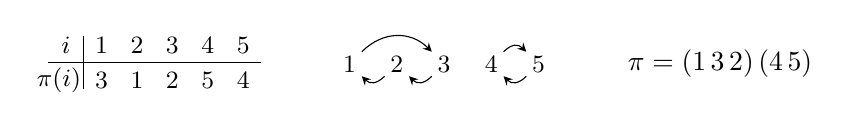
\begin{tikzpicture}[scale=.6,auto]
   \tikzstyle{n} = [inner sep=1pt]
   \tikzstyle{Left} = [draw,bend left=45,-stealth,shorten >= -2pt,
     shorten <= -2pt]
   \tikzstyle{Right} = [draw,bend right=45,-stealth, shorten >= -2pt,
     shorten <= -2pt]
    \begin{scope}[shift={(5,0)}]
      \tikzstyle{every node}=[font=\small]
      \node (1) at (1,0) {$1$};
      \node (2) at (2,0) {$2$};
      \node (3) at (3,0) {$3$};
      \node (4) at (4,0) {$4$};
      \node (5) at (5,0) {$5$};
      \path [Left] (1) to (3); \path [Left] (3) to (2);
      \path [Left] (2) to (1);
      \path [Left] (4) to (5); \path [Left] (5) to (4);
    \end{scope}
    %%
    \begin{scope}[shift={(0,-.35)},scale=.75]
      \tikzstyle{every node}=[font=\small]
      \draw (-.5,.5) -- (5.5,.5); \draw (.5,-.25) -- (.5,1.25);
      \node at (0,1) {$i$}; \node at (-.2,0) {$\pi(i)$}; 
      \node at (1,1) {$1$}; \node at (1,0) {$3$};
      \node at (2,1) {$2$}; \node at (2,0) {$1$};
      \node at (3,1) {$3$}; \node at (3,0) {$2$};
      \node at (4,1) {$4$}; \node at (4,0) {$5$};
      \node at (5,1) {$5$}; \node at (5,0) {$4$};
    \end{scope} 
    %%
    \begin{scope}[shift={(16,0)}]
      \node [anchor=east] at (0,0) {$\pi=(1\,3\,2)\,(4\,5)$};
    \end{scope}
  \end{tikzpicture}%\caption{Three different way \label{fig2:(123)(45)}
  \]

  \vspace{-2mm}\Pause
  
  The matrix $P_\pi$ permutes the entries of a colum vector:
  \[
  \begin{bmatrix} \Palert{0}&\Palert{0}&\Palert{1}&0&0 \\
    \Palert{1}&\Palert{0}&\Palert{0}&0&0 \\ \Palert{0}&\Palert{1}&\Palert{0}&0&0 \\ 0&0&0&0&1 \\ 0&0&0&1&0 \\
  \end{bmatrix}\vvvvv{\Palert{x_1}}{\Palert{x_2}}{\Palert{x_3}}{x_4}{x_5}=
  \vvvvv{\Palert{x_3}}{\Palert{x_1}}{\Palert{x_2}}{x_5}{x_4},\qquad
  \]

  \Pause
  
  It permutes the entries of a row vector (by coordinates):
  \[
  \begin{bmatrix} \Alert{x_1} & \Alert{x_2} & \Alert{x_3} & x_4 & x_5\end{bmatrix}
    \begin{bmatrix} \Alert{0}&\Alert{0}&\Alert{1}&0&0 \\
      \Alert{1}&\Alert{0}&\Alert{0}&0&0 \\
      \Alert{0}&\Alert{1}&\Alert{0}&0&0 \\ 0&0&0&0&1 \\ 0&0&0&1&0 \\
    \end{bmatrix}
    =\begin{bmatrix} \Alert{x_2} & \Alert{x_3} & \Alert{x_1} & x_5 & x_4\end{bmatrix}.
    \]

\end{frame}  

%%====================================================================
%%====================================================================

\begin{frame}{The symmetric group} %\Pause

  Recall that the \Alert{symmetric group} $S_n$ is the group of all
  $n!$ permutations of $\{1,\dots,n\}$. \medskip
  
  If we number the corners of an $n$-gon, every symmetry
  canonically defines a permutation. \medskip\Pause

  However, not every permutation of the corners necessarily is a
  symmetry, unless $n=3$. \medskip\Pause

  Indeed, every permutation of $\{1,2,3\}$ can be realized as an
  element of $D_3$.

  \smallskip\Pause
  
  %% Triangle with symmetries and two Cayley graphs of S3
  \[
  \begin{tikzpicture}[scale=.67,auto]
    \colorlet{color1}{actBlue}
    \colorlet{color2}{actGreen}
    \colorlet{color3}{cosetPurple}
    %%
    %% Colored triangle with symmetries shown, labeled with S3 elements
    %% 
    \begin{scope}[shift={(-7,-.75)},scale=1.5]
      \draw[dashed,thick,eBlue] (.5,1.5) to (.5,-.8);
      \draw[dashed,thick,ePurple] (-.5,-.307) to (1.5,.921);
      \draw[dashed,thick,eGreen] (-.5,.921) to (1.5,-.307);
      \draw[color1,fill=color1]
      (.5,.307)--(.25,.433)--(.5,.866)--(.75,.433)--cycle;
      \draw[color2,fill=color2] (.5,.307)--(.75,.433)--(1,0)--(.5,0)--cycle;
      \draw[color3,fill=color3] (.5,.307)--(.25,.433)--(0,0)--(.5,0)--cycle;
      \draw [black] (0,0)--(.5,.866)--(1,0)--cycle;
      \draw (.5,.55) node {$\mathbf{1}$}; 
      \draw (.3,.2) node {$\mathbf{2}$};\draw (.7,.2) node {$\mathbf{3}$};
      \node[xBlue] at (.5,1.75) {$(23)$};
      \node[xPurple] at (1.7,1.25) {$(13)$};
      \node[xGreen] at (-.8,1.25) {$(12)$};
      \draw[-stealth',eRed] (1.5,-.5) to[thick,bend right=60] (1.7,.2);
      \node at (2.2,-.5) {\color{xRed}$(123)$};
    \end{scope}
    %%
    %% Cayley graph of S_3 = <(123), (23)>
    %%
    \begin{scope}[shift={(0,0)},scale=.9]
      \tikzstyle{v} = [circle, draw, fill=lightgray,inner sep=0pt, 
      minimum size=4.65mm]
      \tikzstyle{every node}=[font=\tiny]
      \tikzstyle{r-in} = [draw, very thick, eRed,-stealth,bend left=35]
      \tikzstyle{r-out} = [draw, very thick, eRed,-stealth,bend right=48]
      %%
      \node (e) at (0:2.4) [v] {\footnotesize $e$};
      \node (r) at (120:2.4) [v] {$(123)$};
      \node (r2) at (240:2.4) [v] {$(132)$};
      \node (f) at (0:1) [v] {$(23)$};
      \node (r2f) at (240:1) [v] {$(12)$};
      \node (rf) at (120:1) [v] {$(13)$};
      \draw [r-out] (e) to  (r);
      \draw [r-out] (r) to (r2);
      \draw [r-out] (r2) to (e);
      \draw [r-in] (f) to (r2f);
      \draw [r-in] (r2f) to (rf);
      \draw [r-in] (rf) to (f);
      \draw [bb] (e) to (f);
      \draw [bb] (r) to (rf);
      \draw [bb] (r2) to (r2f);
    \end{scope}
    %%
    %% Cayley graph of S_3 = <(12), (23)>
    %%
    \begin{scope}[shift={(6,0)}]
      \tikzstyle{v} = [circle, draw, fill=lightgray,inner sep=0pt, 
        minimum size=4.75mm]
      \tikzstyle{every node}=[font=\tiny]
      \node (e) at (90:2) [v] {\footnotesize $e$};
      \node (t) at (30:2) [v] {$(23)$};
      \node (ts) at (-30:2) [v] {$(123)$};
      \node (sts) at (-90:2) [v] {$(13)$};
      \node (st) at (-150:2) [v] {$(132)$};
      \node (s) at (150:2) [v] {$(12)$};
      \path[bb] (e) to (t);
      \path[gg] (t) to (ts);
      \path[bb] (ts) to (sts);
      \path[gg] (st) to (sts);
      \path[bb] (s) to (st);
      \path[gg] (e) to (s);
    \end{scope}
  \end{tikzpicture}
  \]

  \Pause
  
  \begin{exampleblock}{Remark}
    The groups $D_n$ and $S_n$ are isomorphic for $n=3$, and
    non-isomorphic if $n>3$.
  \end{exampleblock}

\end{frame}

%%====================================================================

\begin{frame}{The symmetric group} %\smallskip

  Instead of using configurations of the triangle, consider
  rearrangements of numbers:
  \[
  \big\{\textbf{123},\;\textbf{132},\;\textbf{213},\;\textbf{231},\;
  \textbf{312},\;\textbf{321}\big\}.
  \]
  \Pause Clearly, $S_3$ canonically rearranges these
  configurations. \medskip\Pause
  
  However, \emph{there are two perfectly acceptable interpretations for 
    ``canonical.''} \medskip\pause
  
  For example, \Galert{$(12)$} can be interpreted to mean
  \begin{center}
    ``\emph{swap the numbers in the $1^{\rm st}$ and $2^{\rm nd}$
      \Alert{coordinates}}.''
  \end{center}
  \pause Alternatively, \Galert{$(12)$} could mean
  \begin{center}
    ``\emph{swap the {\color{xPurple}numbers} $1$ and $2$, regardless
      of where they are}.''
  \end{center}
  
  \vspace{-6mm}\pause
  
  % Three Cayley graphs of S_3, and two labelings by configurations
  \[
  \begin{tikzpicture}[scale=.66,auto]
    \tikzstyle{v} = [circle, draw, fill=lightgray,inner sep=0pt, 
      minimum size=4.75mm]
    %%
    %% Cayley graph of S_3 = <(12),(23)>, nodes labeled by elements
    %%
    \begin{scope}[shift={(0,0)}]
      \tikzstyle{every node}=[font=\tiny]
      \node (e) at (90:2) [v] {\footnotesize $e$};
      \node (t) at (150:2) [v] {$(12)$};
      \node (ts) at (-150:2) [v] {$(132)$};
      \node (sts) at (-90:2) [v] {$(13)$};
      \node (st) at (-30:2) [v] {$(123)$};
      \node (s) at (30:2) [v] {$(23)$};
      \path[gg] (e) to (t);
      \path[bb] (t) to (ts);
      \path[gg] (ts) to (sts);
      \path[bb] (st) to (sts);
      \path[gg] (s) to (st);
      \path[bb] (e) to (s);
      \node at (0,.4) {\footnotesize
        $S_3=\big\<\Galert{(12)},\Balert{(23)}\big\>$};
      \node at (0,-.4) {\footnotesize \Alert{right Cayley graph}};
    \end{scope}
    %%
    %% Cayley graph of S_3 = <(12),(23)>, nodes labeled by permutations of 123
    %%
    \begin{scope}[shift={(6,0)},shorten >= -2pt, shorten <= -2pt]
      \tikzstyle{every node}=[font=\small]
      \node (e) at (90:2) {$\mathbf{\underline{123}}$};
      \node (t) at (150:2) {$\mathbf{213}$};
      \node (ts) at (-150:2) {$\mathbf{312}$};
      \node (sts) at (-90:2) {$\mathbf{321}$};
      \node (st) at (-30:2) {$\mathbf{231}$};
      \node (s) at (30:2) {$\mathbf{132}$};
      \path[gg] (e) to (t);
      \path[bb] (t) to (ts);
      \path[gg] (ts) to (sts);
      \path[bb] (st) to (sts);
      \path[gg] (s) to (st);
      \path[bb] (e) to (s);
      \node at (0,0) {``\emph{\color{xPurple}swap numbers}''};
    \end{scope}
    %%
    %% Cayley graph of S_3 = <(12),(23)>, nodes labeled by permutations of 123
    %%
    \begin{scope}[shift={(12,0)},shorten >= -2pt, shorten <= -2pt,]
      \tikzstyle{every node}=[font=\small]
      \node (e) at (90:2) {$\mathbf{\underline{123}}$};
      \node (t) at (150:2) {$\mathbf{213}$};
      \node (ts) at (-150:2) {$\mathbf{231}$};
      \node (sts) at (-90:2) {$\mathbf{321}$};
      \node (st) at (-30:2) {$\mathbf{312}$};
      \node (s) at (30:2) {$\mathbf{132}$};
      \path[gg] (e) to (t);
      \path[bb] (t) to (ts);
      \path[gg] (ts) to (sts);
      \path[bb] (st) to (sts);
      \path[gg] (s) to (st);
      \path[bb] (e) to (s);
      \node at (0,0) {``\emph{\Alert{swap coordinates}}''};
    \end{scope}
  \end{tikzpicture}
  \]
  
  \vspace{-2mm}\Pause Later, we will understand this difference as a
         {\color{xPurple}left group action} vs. a \Alert{right group action}.
         
\end{frame}

%%====================================================================

\begin{frame}{Permutation matrices} 

  \begin{block}{Definition}
    Given an element $\pi\in S_n$, the corresponding \Alert{permutation
      matrix} is the $n\times n$ matrix \vspace{-1mm}
    \[
    P_\pi=(p_{ij}),\qquad p_{ij}=\begin{cases}1 & \pi(i)=j \\ 0 &
    \text{otherwise}. \end{cases}
    \]                    
  \end{block}

  \smallskip\Pause
  
  Here are several more examples of permutation matrices.
  \[
  P_{(12)(34)}=\begin{bmatrix}
  0 & 1 & 0 & 0 \\ 1 & 0 & 0 & 0 \\ 0 & 0 & 0 & 1 \\ 0 & 0 & 1 & 0
  \end{bmatrix},\quad\;\;\Pause
  P_{(134)}=\begin{bmatrix}
  0 & 0 & 1 & 0 \\ 0 & 1 & 0 & 0 \\ 0 & 0 & 0 & 1 \\ 1 & 0 & 0 & 0
  \end{bmatrix},\quad\;\;\Pause
  P_{(1234)}=\begin{bmatrix}
  0 & 1 & 0 & 0 \\ 0 & 0 & 1 & 0 \\ 0 & 0 & 0 & 1 \\ 1 & 0 & 0 & 0
  \end{bmatrix}.
  \]

  \Pause
  
  Notice that the difference between left and right multiplication is:
  \[
  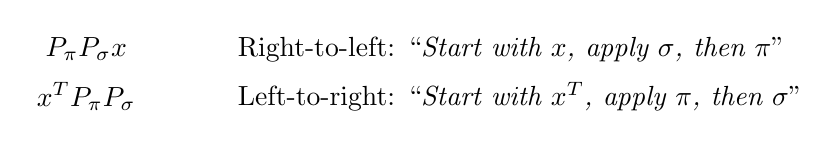
\begin{tikzpicture}[scale=.6,auto]
    \node at (0,0) {$P_\pi P_\sigma x$};
    \node[anchor=west] at (3,0) {\Palert{Right-to-left}:
      ``\emph{Start with $x$, apply $\sigma$, then $\pi$}''};
    \node at (0,-1) {$x^TP_\pi P_\sigma$};
    \node[anchor=west] at (3,-1) {\Alert{Left-to-right}:
      ``\emph{Start with $x^T$, apply $\pi$, then $\sigma$}''};
  \end{tikzpicture}
  \]
  
  \vspace{-2mm}\Pause
  
  It does not matter whether we use row or column vectors, but we must
  be careful. \Pause
  
  \begin{itemize}
  \item \Palert{Column vectors} correspond to multiplying
    \Palert{right-to-left}, as in \Palert{function
      composition}. \smallskip\Pause
  \item \Alert{Row vectors} correspond to multiplying
    \Alert{left-to-right}, which has been \Alert{our standard}.
  \end{itemize}
  
\end{frame}

%%====================================================================

\begin{frame}{\large Our left-to-right multiplication convention is more
    compatible with row vectors}

  \[
  \Galert{P_{(12)}}\Balert{P_{(23)}}\mathbf{v}=
  \Galert{\begin{bmatrix} 0&1&0 \\ 1&0&0 \\ 0&0&1 \end{bmatrix}}
  \Balert{\begin{bmatrix} 1&0&0 \\ 0&0&1 \\ 0&1&0 \end{bmatrix}}
  \vvv{x_1}{x_2}{x_3}\Pause=\Palert{\begin{bmatrix} 0&0&1 \\ 1&0&0 \\ 0&1&0
    \end{bmatrix}\vvv{x_1}{x_2}{x_3}}\Pause=\Palert{\vvv{x_3}{x_1}{x_2}}
  =P_{(132)}\mathbf{v}.
  \]

  \vspace{-2mm}\Pause

  \[
  \begin{array}{c@{\hspace{1mm}}c@{\hspace{1mm}}l}
    \mathbf{v}^T\Galert{P_{(12)}}\Balert{P_{(23)}}
    =\begin{bmatrix} x_1 & x_2 & x_3 \end{bmatrix}
    \Galert{\begin{bmatrix} 0&1&0 \\ 1&0&0 \\ 0&0&1 \end{bmatrix}}
    \Balert{\begin{bmatrix} 1&0&0 \\ 0&0&1 \\ 0&1&0 \end{bmatrix}} \Pause
    &=&\Alert{\begin{bmatrix} x_1 & x_2 & x_3 \end{bmatrix}
      \begin{bmatrix} 0&0&1 \\ 1&0&0 \\ 0&1&0 \end{bmatrix}} 
    \vspace{2mm}\Pause \\ &=&\Alert{\begin{bmatrix} x_2 & x_3 &
        x_1 \end{bmatrix}}=\mathbf{v}^TP_{(132)}.
  \end{array}
  \]
  
  \vspace{-4mm}\Pause

  
  % Cayley graphs of S_3, and two labelings by configurations
  \[
  \begin{tikzpicture}[scale=.75,auto]
  \tikzstyle{v} = [circle, draw, fill=lightgray,inner sep=0pt, 
    minimum size=4.5mm]
  %%
  %% Cayley graph of S_3=<(12),(23)> with nodes labeled by group elements
  %%
  \begin{scope}[shift={(0,0)}]
      \tikzstyle{every node}=[font=\tiny]
      \node (e) at (90:2) [v] {\footnotesize $e$};
      \node (t) at (150:2) [v] {$(12)$};
      \node (ts) at (-150:2) [v] {\Alert{$(132)$}};
      \node (sts) at (-90:2) [v] {$(13)$};
      \node (st) at (-30:2) [v] {$(123)$};
      \node (s) at (30:2) [v] {$(23)$};
      \path[gg] (e) to (t);
      \path[bb] (t) to (ts);
      \path[gg] (ts) to (sts);
      \path[bb] (st) to (sts);
      \path[gg] (s) to (st);
      \path[bb] (e) to (s);
      \node at (0,.4) {\small $S_3=\big\<\Galert{(12)},\Balert{(23)}\big\>$};
      \node at (0,-.4) {\small \Alert{right Cayley graph}};
  \end{scope}
  %%
  %% Cayley graph of S_3=<(12),(23)> with nodes labeled by column vectors
  %%
  \begin{scope}[shift={(5.5,0)},shorten >= -2pt, shorten <= -2pt]
    \tikzstyle{every node}=[font=\footnotesize]
    \node (e) at (90:2) {$\vvv{x_1}{x_2}{x_3}$};
    \node (t) at (150:2) {$\vvv{x_2}{x_1}{x_3}$};
    \node (sts) at (-90:2) {$\vvv{x_3}{x_2}{x_1}$};
    \node (ts) at (-150:2) {$\vvv{x_3}{x_1}{x_2}$};
    \node (st) at (-30:2) {$\vvv{x_2}{x_3}{x_1}$};
    \node (s) at (30:2) {$\vvv{x_1}{x_3}{x_2}$};
    \path[gg] (e) to (t);
    \path[bb] (t) to (ts);
    \path[gg] (ts) to (sts);
    \path[bb] (st) to (sts);
    \path[gg] (s) to (st);
    \path[bb] (e) to (s);
    \node at (0,.4) {\small \Palert{$f(g(x))\neq (fg)(x)$)}};
    \node at (0,-.4) {\small ``\emph{\Palert{swap numbers}''}};
  \end{scope}
  %%
  %% Cayley graph of S_3=<(12),(23)> with nodes labeled by row vectors
  %%
  \begin{scope}[shift={(11,0)},shorten >= -2pt, shorten <= -2pt,]
    \tikzstyle{every node}=[font=\footnotesize]
    \node (e) at (90:2) {$[x_1\;x_2\;x_3]$};
    \node (t) at (150:2) {$[x_2\;x_1\;x_3]$};
    \node (ts) at (-150:2) {$[x_2\;x_3\;x_1]$};
    \node (sts) at (-90:2) {$[x_3\;x_2\;x_1]$};
    \node (st) at (-30:2) {$[x_3\;x_1\;x_2]$};
    \node (s) at (30:2) {$[x_1\;x_3\;x_2]$};
    \path[gg] (e) to (t);
    \path[bb] (t) to (ts);
    \path[gg] (ts) to (sts);
    \path[bb] (st) to (sts);
    \path[gg] (s) to (st);
    \path[bb] (e) to (s);
    \node at (0,.4) {\small \Alert{$((x)f)g=(x)(fg)$}};
    \node at (0,-.4) {\small ``\emph{\Alert{swap coordinates}}''};
  \end{scope}
  \end{tikzpicture}
  \]
  
\end{frame}

%%====================================================================

\begin{frame}{Polytopes and platonic solids} %\Pause
  
  A \Alert{polytope} is a finite region of $\R^n$ enclosed by
  finitely many hyperplanes. \bigskip\Pause

  2D polytopes are \emph{polygons}, and 3D polytopes are
  \Alert{polyhedra}. \bigskip\Pause
  
  The formal definition of a \Alert{regular polytope} involves a
  technical condition of its symmetry group. \bigskip\Pause


  Informally, it means all faces and all vertices are
  identical and indistinguishable -- higher-dimensional analogues of
  regular polygons. \bigskip\Pause

  There are exactly five regular polyhedra, called
  \Alert{Platonic solids}.

  \begin{center}
    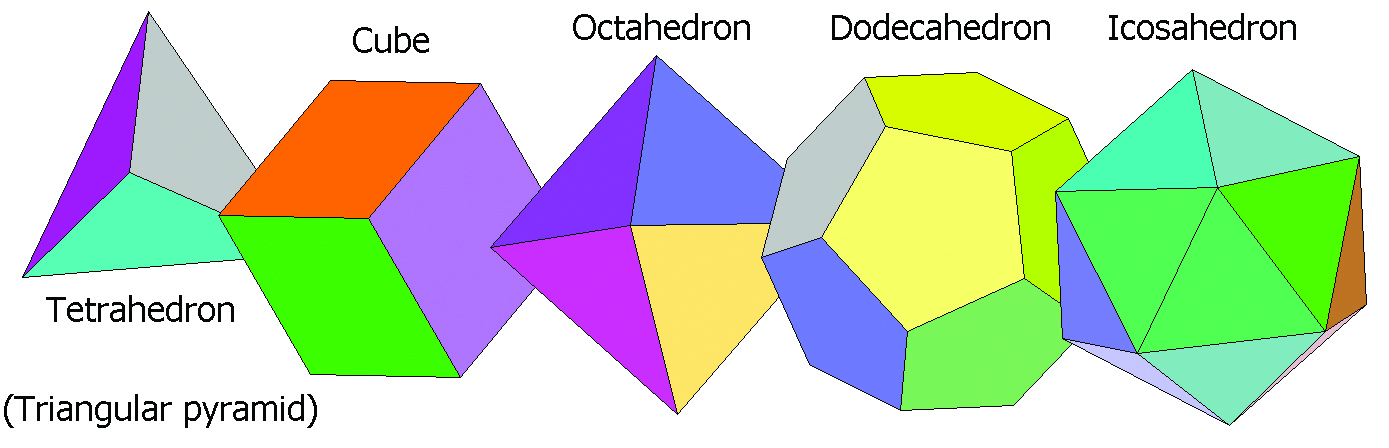
\includegraphics[width=.8\textwidth]{platonic-solids}
  \end{center}

\end{frame}

%%====================================================================

\begin{frame}{Archimedean solids} %\Pause
  
  More general than the Platonic solids are the \Alert{Archimedean
    solids}. \bigskip\Pause

  These are non-regular \Balert{convex uniform polyhedra} built from
  regular polygons.

  \bigskip\Pause
  
  Though they can involve different polygons, all vertices are
  locally identical.

  \bigskip\Pause

  In the third century B.C.E., Archimedes classified all 13 such polyhedra.
  
  \bigskip\Pause

  Five are ``truncated versions'' of the Platonic solids -- formed
  by chopping off vertices.

  \bigskip\Pause

  The others consist of \smallskip
  \begin{itemize}
  \item the chiral ``\Balert{snub cube}'' and ``\Balert{snub
    dodecahedron}'' \smallskip\Pause
  \item ``hybrids'' such as the \Balert{icosidodecahedron} \smallskip\Pause
  \item truncated versions of these hybrids.
  \end{itemize}
  
  \bigskip\Pause
  
  The Cayley graph of $S_4$ can be arranged on the skeletons of
  several of these. 
    
\end{frame}

%%====================================================================

\begin{frame}%{Archimedean solids} %\Pause

  \begin{center}
    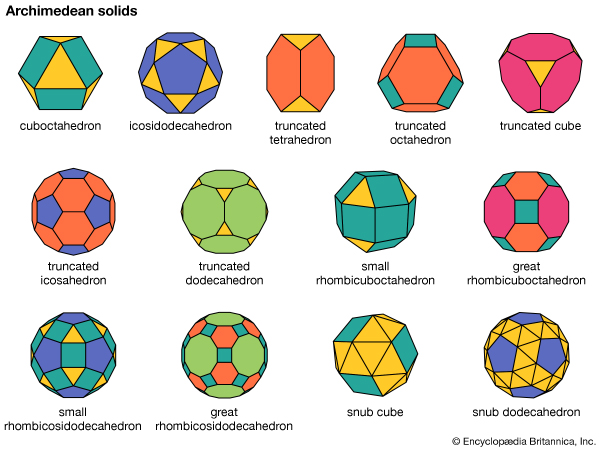
\includegraphics[width=1\textwidth]{archimedean-solids.jpg}
  \end{center}
  
\end{frame}

%%====================================================================

\begin{frame}{The left and right permutahedra} \smallskip

  \begin{block}{Definition}
    The \Alert{$n$-permutahedron} is the convex hull of the $n!$
    permutations of $(1,\dots,n)\in\R^n$.
  \end{block}

  \smallskip\Pause

  This is an $(n-1)$-dimensional polytope, as it lies on the
  hyperplane $x_1+\cdots+x_n=\frac{(n-1)n}{2}$. \Pause It is also the
  Cayley graph of
  \[
  S_4=\big\<\Galert{(12)},\;\Balert{(23)},\;\Alert{(34)}\big\>.
  \]
  
  \vspace{-5mm}

  %% A Cayley graph of S4 = <(12),(23),(34)> on the skeleton of the
  %% 4-permutahedron twice. One where edges are defined by "swapping coords",
  %% and the other defined by "swapping numbers"
  \[
  \begin{tikzpicture}[shorten >= -3pt, shorten <= -3pt,scale=.7]
    \tikzstyle{every node}=[font=\tiny]
    %%
    %% 4-permutahedron with edges defined by swapping coordinates
    %%
    \begin{scope}[shift={(0,0)},scale=.18]
      \node (3124) at (12.15,35.1) {$2314$}; %%
      \node (4123) at (23,35.8) {$2341$}; %%
      \node (4213) at (28.2,35.1) {$3241$};
      \node (3214) at (17,34.35) {$3214$};
      \node (4132) at (25.5,29.2) {\color{midgray} $2431$}; % 
      \node (2134) at (4.15,27.15) {$2134$};
      \node (4312) at (36.2,27.15) {$3421$}; %%
      \node (2314) at (13.5,24.6) {$3124$}; %%
      \node (4231) at (32.8,21.9) {\color{midgray} $4231$};       
      \node (3142) at (18.3,20.8) {\color{midgray} $2413$}; %%    %!!!
      \node (2143) at (7.7,20.6) {\color{midgray} $2143$};        %!!!
      \node (4321) at (38.2,20.6) {$4321$};
      %%
      \node (1234) at (.2,17.5) {$1234$};
      \node (3412) at (33.9,17.5) {$3412$};
      \node (3241) at (25.5,14.6) {\color{midgray} $4213$}; %%     %!!!
      \node (1243) at (4.15,11.1) {$1243$};               %!!!
      \node (3421) at (36.2,11.1) {$4312$}; %%
      \node (1423) at (13.5,6.8) {$1342$}; %%
      \node (2341) at (23,5.3) {\color{midgray} $4123$}; %%   
      \node (1342) at (12.2,3.1) {$1423$}; %%
      \node (2431) at (28.1,3.1) {$4132$}; %%
      \node (1432) at (17,.6) {$1432$};
      %%
      \draw [ggFaded] (3142) -- (3241); %!!!
      \draw [ggFaded] (2143) -- (1243); %!!!
      \node (1324) at (4.7,15.7) {$1324$};  %%TOP
      \node (2413) at (22.4,15.7) {$3142$}; %%TOP
      %%
      \draw [rrFaded] (4132) -- (3142);
      \draw [rrFaded] (2134) -- (2143);
      \draw [rrFaded] (4231) -- (3241);
      \draw [rrFaded] (2341) -- (2431);
      \draw [ggFaded] (4132) -- (4231);
      \draw [ggFaded] (2341) -- (1342);
      \draw [bbFaded] (4123) -- (4132);
      \draw [bbFaded] (4231) -- (4321);
      \draw [bbFaded] (3142) -- (2143); 
      \draw [bbFaded] (3241) -- (2341);
      %%
      \draw [rr] (3124) -- (4123);
      \draw [rr] (3214) -- (4213);
      \draw [rr] (4312) -- (3412);
      \draw [rr] (2314) -- (2413);
      \draw [rr] (4321) -- (3421);
      \draw [rr] (1234) -- (1243);
      \draw [rr] (1324) -- (1423);
      \draw [rr] (1342) -- (1432);
      %%
      \draw [gg] (3124) -- (3214);
      \draw [gg] (2134) -- (1234);
      \draw [gg] (4312) -- (4321);
      \draw [gg] (2314) -- (1324);
      \draw [gg] (3412) -- (3421); 
      \draw [gg] (2413) -- (1423);
      \draw [gg] (2431) -- (1432);
      \draw [gg] (4123) -- (4213);
      %%
      \draw [bb] (3124) -- (2134);
      \draw [bb] (4213) -- (4312);
      \draw [bb] (3214) -- (2314);
      \draw [bb] (1234) -- (1324);
      \draw [bb] (3412) -- (2413);
      \draw [bb] (1243) -- (1342);
      \draw [bb] (3421) -- (2431);
      \draw [bb] (1423) -- (1432);
      \node at (19,-4) {\normalsize``\emph{swap coordinates}''};
    \end{scope}
    %%
    %% 4-permutahedron with edges defined by swapping numbers
    %%
    \begin{scope}[shift={(8.75,0)},scale=.18]
      \node (3124) at (12.15,35.1) {$3124$};
      \node (4123) at (23,35.8) {$4123$};
      \node (4213) at (28.2,35.1) {$4213$};
      \node (3214) at (17,34.35) {$3214$};
      \node (4132) at (25.5,29.2) {\color{midgray} $4132$}; %
      \node (2134) at (4.15,27.15) {$2134$};
      \node (4312) at (36.2,27.15) {$4312$};
      \node (2314) at (13.5,24.6) {$2314$};
      \node (4231) at (32.8,21.9) {\color{midgray} $4231$}; %
      \node (3142) at (18.3,20.8) {\color{midgray} $3142$}; %
      \node (2143) at (7.7,20.6) {\color{midgray} $2143$}; %
      \node (4321) at (38.2,20.6) {$4321$};
      %%
      \node (1234) at (.2,17.5) {$1234$};
      \node (3412) at (33.9,17.5) {$3412$};
      \node (3241) at (25.5,14.6) {\color{midgray} $3241$}; %
      \node (1243) at (4.15,11.1) {$1243$};
      \node (3421) at (36.2,11.1) {$3421$};
      \node (1423) at (13.5,6.8) {$1423$};
      \node (2341) at (23,5.3) {\color{midgray} $2341$}; %
      \node (1342) at (12.2,3.1) {$1342$};
      \node (2431) at (28.1,3.1) {$2431$};
      \node (1432) at (17,.6) {$1432$};
      %%
      \draw [ggFaded] (3142) -- (3241);
      \draw [ggFaded] (2143) -- (1243);
      \node (1324) at (4.7,15.7) {$1324$};
      \node (2413) at (22.4,15.7) {$2413$};
      %%
      \draw [rrFaded] (4132) -- (3142);
      \draw [rrFaded] (2134) -- (2143);
      \draw [rrFaded] (4231) -- (3241);
      \draw [rrFaded] (2341) -- (2431);
      \draw [ggFaded] (4132) -- (4231);
      \draw [ggFaded] (2341) -- (1342);
      \draw [bbFaded] (4123) -- (4132);
      \draw [bbFaded] (4231) -- (4321);
      \draw [bbFaded] (3142) -- (2143);
      \draw [bbFaded] (3241) -- (2341);
      %%
      \draw [rr] (3124) -- (4123);
      \draw [rr] (3214) -- (4213);
      \draw [rr] (4312) -- (3412);
      \draw [rr] (2314) -- (2413);
      \draw [rr] (4321) -- (3421);
      \draw [rr] (1234) -- (1243);
      \draw [rr] (1324) -- (1423);
      \draw [rr] (1342) -- (1432);
      %%
      \draw [gg] (3124) -- (3214);
      \draw [gg] (2134) -- (1234);
      \draw [gg] (4312) -- (4321);
      \draw [gg] (2314) -- (1324);
      \draw [gg] (3412) -- (3421); 
      \draw [gg] (2413) -- (1423);
      \draw [gg] (2431) -- (1432);
      \draw [gg] (4123) -- (4213);
      %%
      \draw [bb] (3124) -- (2134);
      \draw [bb] (4213) -- (4312);
      \draw [bb] (3214) -- (2314);
      \draw [bb] (1234) -- (1324);
      \draw [bb] (3412) -- (2413);
      \draw [bb] (1243) -- (1342);
      \draw [bb] (3421) -- (2431);
      \draw [bb] (1423) -- (1432);
      \node at (19,-4) {\normalsize``\emph{swap numbers}''};
    \end{scope}
  \end{tikzpicture}
  \]

\end{frame}

%%====================================================================

\begin{frame}{The appearance of $A_4$ in Cayley graphs for $S_4$} \smallskip
  
  Let's highlight in yellow the even permutations in Cayley graphs
  for $S_4$.
    
  \vspace{-3mm}

  %% Cayley graphs of S_4: on a permutahedron and Nauru graph
  \[
  \begin{tikzpicture}[scale=.65]
    \tikzstyle{v} = [circle, draw, fill=lightgray,inner sep=0pt,
      minimum size=2.25mm]
    \tikzstyle{v-yel} = [circle, draw, fill=yellow,inner sep=0pt,
      minimum size=2.25mm]
    \tikzstyle{v-yelf} = [circle, draw, fill=vYellow,inner sep=0pt,
      minimum size=2.25mm] 
    \tikzstyle{v-f} = [circle, draw, gray, fill=lightgray,inner sep=0pt,
      minimum size=2.25mm]
    %%
    %% Cayley graphs of S_4 on a truncated cube
    %%
    \begin{scope}[scale=.2]
      \node (3124) at (12.15,35.1) [v-yel] {};
      \node (4123) at (23,35.8) [v] {};
      \node (4213) at (28.2,35.1) [v-yel] {};
      \node (3214) at (17,34.35) [v] {};
      \node (4132) at (25.5,29.2) [v-yelf] {};
      \node (2134) at (4.15,27.15) [v] {};
      \node (4312) at (36.2,27.15) [v] {};
      \node (2314) at (13.5,24.6) [v-yel] {};
      \node (4231) at (32.8,21.9) [v-f] {};
      \node (3142) at (18.3,20.8) [v-f] {};
      \node (2143) at (7.7,20.6) [v-yelf] {};
      \node (4321) at (38.2,20.6) [v-yel] {};
      %%
      \node (1234) at (.2,17.5) [v-yel] {\footnotesize $e$};
      \node (3412) at (33.9,17.5) [v-yel] {};
      \node (1324) at (4.7,15.7) [v] {};
      \node (2413) at (22.4,15.7) [v] {};
      \node (3241) at (25.5,14.6) [v-yelf] {};
      \node (1243) at (4.15,11.1) [v] {};
      \node (3421) at (36.2,11.1) [v] {};
      \node (1423) at (13.5,6.8) [v-yel] {};
      \node (2341) at (23,5.3) [v-f] {};
      \node (1342) at (12.2,3.1) [v-yel] {};
      \node (2431) at (28.1,3.1) [v-yel] {};
      \node (1432) at (17,.6) [v] {};
      %%
      \draw [rrFaded] (4132) to (3142);
      \draw [rrFaded] (2134) to (2143);
      \draw [rrFaded] (4231) to (3241);
      \draw [rrFaded] (2341) to (2431);
      \draw [ggFaded] (4132) to (4231);
      \draw [ggFaded] (3142) to (3241);
      \draw [ggFaded] (2143) to (1243);
      \draw [ggFaded] (2341) to (1342);
      \draw [bbFaded] (4123) to (4132);
      \draw [bbFaded] (4231) to (4321);
      \draw [bbFaded] (3142) to (2143);
      \draw [bbFaded] (3241) to (2341);
      %%
      \draw [rr] (3124) to (4123);
      \draw [rr] (3214) to (4213);
      \draw [rr] (4312) to (3412);
      \draw [rr] (2314) to (2413);
      \draw [rr] (4321) to (3421);
      \draw [rr] (1234) to (1243);
      \draw [rr] (1324) to (1423);
      \draw [rr] (1342) to (1432);
      %%
      \draw [gg] (3124) to (3214);
      \draw [gg] (2134) to (1234);
      \draw [gg] (4312) to (4321);
      \draw [gg] (2314) to (1324);
      \draw [gg] (3412) to (3421); 
      \draw [gg] (2413) to (1423);
      \draw [gg] (2431) to (1432);
      \draw [gg] (4123) to (4213);
      %%
      \draw [bb] (3124) to (2134);
      \draw [bb] (4213) to (4312);
      \draw [bb] (3214) to (2314);
      \draw [bb] (1234) to (1324);
      \draw [bb] (3412) to (2413);
      \draw [bb] (1243) to (1342);
      \draw [bb] (3421) to (2431);
      \draw [bb] (1423) to (1432);
      \node at (19,40) {$S_4=\big\<\Galert{(12)},\;\Balert{(23)},
        \;\Alert{(34)}\big\>$};
      \node at (19,-4) {truncated octahedron; ``\emph{permutahedron}''};
    \end{scope}
    %%
    %% Cayley graphs of S_4 on the Nauru graph
    %%
    \begin{scope}[shift={(13.25,3.6)},scale=1.75]
      \node (4321) at (0:1) [v] {};
      \node (3142) at (30:1) [v-yel] {};
      \node (2314) at (60:1) [v] {};
      \node (1432) at (90:1) [v-yel] {};
      \node (4213) at (120:1) [v] {};
      \node (3421) at (150:1) [v-yel] {};
      \node (2143) at (180:1) [v] {};
      \node (1324) at (210:1) [v-yel] {};
      \node (4132) at (240:1) [v] {};
      \node (3214) at (270:1) [v-yel] {};
      \node (2431) at (300:1) [v] {};
      \node (1243) at (330:1) [v-yel] {};
      %%
      \node (2341) at (0:2) [v-yel] {\footnotesize $e$};
      \node (1342) at (30:2) [v] {};
      \node (4312) at (60:2) [v-yel] {};
      \node (3412) at (90:2) [v] {};
      \node (2413) at (120:2) [v-yel] {};
      \node (1423) at (150:2) [v] {};
      \node (4123) at (180:2) [v-yel] {};
      \node (3124) at (210:2) [v] {};
      \node (2134) at (240:2) [v-yel] {};
      \node (1234) at (270:2) [v] {};
      \node (4231) at (300:2) [v-yel] {};
      \node (3241) at (330:2) [v] {};
      %%
      \draw [bb] (1432) to (2431); \draw [bb] (4213) to (3214);
      \draw [bb] (2143) to (3142); \draw [bb] (1324) to (4321);
      \draw [bb] (2413) to (3412); \draw [bb] (1342) to (2341);
      \draw [bb] (4231) to (1234); \draw [bb] (3124) to (4123);
      \draw [bb] (2314) to (4312); \draw [bb] (1243) to (3241);
      \draw [bb] (4132) to (2134); \draw [bb] (3421) to (1423);
      %%
      \draw [oo] (1432) to (4132); \draw [oo] (2314) to (3214);
      \draw [oo] (3421) to (4321); \draw [oo] (2143) to (1243);
      \draw [oo] (3412) to (4312); \draw [oo] (2134) to (1234);
      \draw [oo] (2341) to (3241); \draw [oo] (4123) to (1423);
      \draw [oo] (4213) to (2413); \draw [oo] (2431) to (4231);
      \draw [oo] (1324) to (3124); \draw [oo] (3142) to (1342);
      %%
      \draw [gg] (4213) to (1243); \draw [gg] (3421) to (2431);
      \draw [gg] (1324) to (2314); \draw [gg] (4132) to (3142);
      \draw [gg] (4312) to (1342); \draw [gg] (2134) to (3124);
      \draw [gg] (1423) to (2413); \draw [gg] (4231) to (3241);
      \draw [gg] (1432) to (3412); \draw [gg] (3214) to (1234);
      \draw [gg] (2143) to (4123); \draw [gg] (4321) to (2341);
      \node at (90:2.5) {$S_4=\big\<{\color{xGreen}(12)},{\color{xBlue}(13)}
        ,{\color{xOrange}(14)}\big\>$};
      \node at (270:2.5) {``\emph{Nauru graph}''};
    \end{scope}
  \end{tikzpicture}
  \]
  
  \Pause
  
  Notice that any two paths between yellow nodes has
  \textbf{\textit{even length}}.
 
\end{frame}

%%====================================================================

\begin{frame}{The appearance of $A_4$ in Cayley graphs for $S_4$} \smallskip

  
  There are only five $\textbf{\textit{cycle types}}$ in $S_4$:
  \begin{center}
    \begin{tabular}{c|ccccc}
      example element & $e$ & \Palert{$(12)$} & \Alert{$(234)$} &
      \Balert{$(1234)$} & $(12)(34)$ \\ \hline
      parity & even & \Palert{odd} & \Alert{even} & \Balert{odd} &
      even \\ \# elts & 1 & \Palert{6} & \Alert{8} & \Balert{6} & 3
    \end{tabular}
  \end{center}
  
  \Pause
  
  In both Cayley graphs, blue arrows flip the sign of the permutation;
  red arrows do not. \medskip

  Once again, even permutations are highlighted in yellow.

  
  %% Cayley graphs of S_4 on the truncated cube and the rhombicuboctahedron
  \[
  \begin{tikzpicture}[scale=.65]
    \tikzstyle{v} = [circle, draw, fill=lightgray,inner sep=0pt, 
      minimum size=2.25mm]
    \tikzstyle{v-y} = [circle, draw, fill=yellow,inner sep=0pt, 
      minimum size=2.25mm]
    \newcommand\aaa{1}\newcommand\bbb{2}\newcommand\ccc{3}\newcommand\ddd{4.6}
    %%
    %% Cayley graph of S_4 on the truncated cube
    %%
    \begin{scope}[shift={(0,0)}]
      \node (nw1) at (-1.5,1.5) [v-y] {\footnotesize $e$};
      \node (nw2) at (-.5,1.5) [v-y] {}; 
       \node (nw3) at (-1.5,.5) [v-y] {};
       \node (ne1) at (1.5,1.5) [v] {};
       \node (ne2) at (1.5,.5) [v] {}; 
       \node (ne3) at (.5,1.5) [v] {};
       \node (se1) at (1.5,-1.5) [v-y] {};
       \node (se2) at (.5,-1.5) [v-y] {};
       \node (se3) at (1.5,-.5) [v-y] {}; 
       \node (sw1) at (-1.5,-1.5) [v] {};
       \node (sw2) at (-1.5,-.5) [v] {}; 
       \node (sw3) at (-.5,-1.5) [v] {};
       %
       \draw [pp] (nw2) to (ne3); \draw [pp] (ne2) to (se3);
       \draw [pp] (se2) to (sw3); \draw [pp] (sw2) to (nw3);
       \draw[r](nw2)to(nw1); \draw [r] (nw3) to (nw2); \draw [r] (nw1) to (nw3);
       \draw[r](ne2)to(ne1); \draw [r] (ne3) to (ne2); \draw [r] (ne1) to (ne3);
       \draw[r](se2)to(se1); \draw [r] (se3) to (se2); \draw [r] (se1) to (se3);
       \draw[r](sw2)to(sw1); \draw [r] (sw3) to (sw2); \draw [r] (sw1) to (sw3);
       %%
       \node (NW1) at (-2.25,2.25) [v] {};
       \node (NW2) at (-3.25,2.25) [v] {}; 
       \node (NW3) at (-2.25,3.25) [v] {};
       \node (NE1) at (2.25,2.25) [v-y] {};
       \node (NE2) at (2.25,3.25) [v-y] {}; 
       \node (NE3) at (3.25,2.25) [v-y] {};
       \node (SE1) at (2.25,-2.25) [v] {};
       \node (SE2) at (3.25,-2.25) [v] {};
       \node (SE3) at (2.25,-3.25) [v] {}; 
       \node (SW1) at (-2.25,-2.25) [v-y] {};
       \node (SW2) at (-2.25,-3.25) [v-y] {}; 
       \node (SW3) at (-3.25,-2.25) [v-y] {};
       %%
       \draw [pp] (NW3) to (NE2); \draw [pp] (NE3) to (SE2);
       \draw [pp] (SE3) to (SW2); \draw [pp] (SW3) to (NW2);
       %
       \draw[r](NW2)to(NW1); \draw [r] (NW3) to (NW2); \draw [r] (NW1) to (NW3);
       \draw[r](NE2)to(NE1); \draw [r] (NE3) to (NE2); \draw [r] (NE1) to (NE3);
       \draw[r](SE2)to(SE1); \draw [r] (SE3) to (SE2); \draw [r] (SE1) to (SE3);
       \draw[r](SW2)to(SW1); \draw [r] (SW3) to (SW2); \draw [r] (SW1) to (SW3);
       %%
       \draw [pp] (nw1) to (NW1); \draw [pp] (ne1) to (NE1);
       \draw [pp] (se1) to (SE1); \draw [pp] (sw1) to (SW1);
       %
       \node at (0,-4) {\emph{truncated cube}};
    \end{scope}
    %%
    %% Cayley graphs of S_4 on the rhombicuboctahedron
    %%
    \begin{scope}[shift={(9,0)}]
      %%
      \node (ne-1) at (45:\aaa) [v] {};
      \node (ne-2) at (67.5:\bbb) [v] {};
      \node (ne-3) at (22.5:\bbb) [v] {};
      \node (ne-4) at (67.5:\ccc) [v-y] {};
      \node (ne-5) at (22.5:\ccc) [v-y] {};
      \node (ne-6) at (45:\ddd) [v-y] {};
      %%
      \node (nw-1) at (45+90:\aaa) [v-y] {\footnotesize $e$};
      \node (nw-2) at (67.5+90:\bbb) [v-y] {};
      \node (nw-3) at (22.5+90:\bbb) [v-y] {};
      \node (nw-4) at (67.5+90:\ccc) [v] {};
      \node (nw-5) at (22.5+90:\ccc) [v] {};
      \node (nw-6) at (45+90:\ddd) [v] {};
      %%
      \node (se-1) at (45-90:\aaa) [v-y] {};
      \node (se-2) at (67.5-90:\bbb) [v-y] {};
      \node (se-3) at (22.5-90:\bbb) [v-y] {};
      \node (se-4) at (67.5-90:\ccc) [v] {};
      \node (se-5) at (22.5-90:\ccc) [v] {};
      \node (se-6) at (45-90:\ddd) [v] {};
      %%
      \node (sw-1) at (45+180:\aaa) [v] {};
      \node (sw-2) at (67.5+180:\bbb) [v] {};
      \node (sw-3) at (22.5+180:\bbb) [v] {};
      \node (sw-4) at (67.5+180:\ccc) [v-y] {};
      \node (sw-5) at (22.5+180:\ccc) [v-y] {};
      \node (sw-6) at (45+180:\ddd) [v-y] {};
      %%
      \draw [r] (ne-2) to (ne-1); \draw [r] (ne-3) to (ne-2);
      \draw [r] (ne-1) to (ne-3);
      \draw [b] (ne-2) to (ne-4); \draw [b] (ne-5) to (ne-3);
      \draw [r] (ne-4) to (ne-5); \draw [r] (ne-6) to (ne-4);
      \draw [r] (ne-5) to (ne-6);
      %%
      \draw [r] (nw-2) to (nw-1); \draw [r] (nw-3) to (nw-2);
      \draw [r] (nw-1) to (nw-3);
      \draw [b] (nw-2) to (nw-4); \draw [b] (nw-5) to (nw-3);
      \draw [r] (nw-4) to (nw-5); \draw [r] (nw-6) to (nw-4);
      \draw [r] (nw-5) to (nw-6);
      %%
      \draw [r] (se-2) to (se-1); \draw [r] (se-3) to (se-2);
      \draw [r] (se-1) to (se-3);
      \draw [b] (se-2) to (se-4); \draw [b] (se-5) to (se-3);
      \draw [r] (se-4) to (se-5); \draw [r] (se-6) to (se-4);
      \draw [r] (se-5) to (se-6);
      %%
      \draw [r] (sw-2) to (sw-1); \draw [r] (sw-3) to (sw-2);
      \draw [r] (sw-1) to (sw-3);
      \draw [b] (sw-2) to (sw-4); \draw [b] (sw-5) to (sw-3);
      \draw [r] (sw-4) to (sw-5); \draw [r] (sw-6) to (sw-4);
      \draw [r] (sw-5) to (sw-6);
      %%
      \draw [b] (ne-1) to (nw-1); \draw [b] (se-1) to (ne-1);
      \draw [b] (sw-1) to (se-1); \draw [b] (nw-1) to (sw-1);
      %%
      \draw [b] (nw-6) to (ne-6); \draw [b] (sw-6) to (nw-6);
      \draw [b] (se-6) to (sw-6); \draw [b] (ne-6) to (se-6);
      %%
      \draw [b] (ne-4) to (nw-5); \draw [b] (se-4) to (ne-5);
      \draw [b] (sw-4) to (se-5); \draw [b] (nw-4) to (sw-5);
      %%
      \draw [b] (nw-3) to (ne-2); \draw [b] (sw-3) to (nw-2);
      \draw [b] (se-3) to (sw-2); \draw [b] (ne-3) to (se-2);
      \node at (0,-4) {\emph{rhombicuboctahedron}};
     \end{scope}
   \end{tikzpicture}
   \]

\end{frame}

%%====================================================================


\begin{frame}{The cycle graph of $S_4$}
  
  %% The cycle graph of S4
  \[
  \scalebox{.9}{
    \begin{tikzpicture}[scale=1,yscale=1.6]
      \tikzstyle{v-r} = [circle, draw, fill=vRed,inner sep=0pt,
        minimum size=6.5mm]
      \tikzstyle{v-g} = [circle, draw, fill=vGreen,inner sep=0pt,
        minimum size=6.5mm]
      \tikzstyle{v-b} = [circle, draw, fill=vBlue,inner sep=0pt,
        minimum size=6.5mm]
      \tikzstyle{v-p} = [circle, draw, fill=vPurple,inner sep=0pt, 
        minimum size=6.5mm]
      \tikzstyle{v-gr} = [circle, draw, fill=midgray,inner sep=0pt,
        minimum size=6.5mm]
      \begin{scope}
        \tikzstyle{every node}=[font=\scriptsize]
        \node [v-gr] (e) at (0,0) {\normalsize $e$};
        \node [v-r] (123) at (-6,2) {\footnotesize $(123)$};
        \node [v-r] (124) at (-5,2) {\footnotesize $(124)$};
        \node [v-r] (134) at (-4,2) {\footnotesize $(134)$};
        \node [v-r] (234) at (-3,2) {\footnotesize $(234)$};
        \node [v-b] (12-34) at (-1.6,2) {$(\!12\!)(\!34\!)$};
        \node [v-b] (13-24) at (0,2) {$(\!13\!)(\!24\!)$};
        \node [v-b] (14-23) at (1.6,2) {$(\!14)(\!23)$};
        \node [v-r] (132) at (6,2) {\footnotesize $(132)$};
        \node [v-r] (142) at (5,2) {\footnotesize $(142)$};
        \node [v-r] (143) at (4,2) {\footnotesize $(143)$};
        \node [v-r] (243) at (3,2) {\footnotesize $(243)$};
        \node [v-g] (1324) at (-2,1) {$(1324)$};
        \node [v-g] (1423) at (-1.2,1) {$(1423)$};
        \node [v-g] (1234) at (-.4,1) {$(1234)$};
        \node [v-g] (1432) at (.4,1) {$(1432)$};
        \node [v-g] (1243) at (1.2,1) {$(1243)$};
        \node [v-g] (1342) at (2,1) {$(1342)$};
        \node [v-p] (12) at (-3,-1) {\small $(12)$};
        \node [v-p] (34) at (-2,-1) {\small $(34)$};
        \node [v-p] (13) at (-.5,-1) {\small $(13)$};
        \node [v-p] (24) at (.5,-1) {\small $(24)$};
        \node [v-p] (23) at (2,-1) {\small $(23)$};
        \node [v-p] (14) at (3,-1) {\small $(14)$};
        \draw [cy2,out=85,in=95,looseness=.2] (123) to  (132);
        \draw [cy2,out=85,in=95,looseness=.2] (124) to (142);
        \draw [cy2,out=85,in=95,looseness=.2] (134) to (143);
        \draw [cy2,out=85,in=95,looseness=.2] (234) to (243);
        \draw [cy2,bend left=12] (e) to (1324);
        \draw [cy2,bend left=12] (e) to (1423);
        \draw [cy2,bend left=12] (e) to (1234);
        \draw [cy2,bend right=12] (e) to (1432);
        \draw [cy2,bend right=12] (e) to (1243);
        \draw [cy2,bend right=12] (e) to (1342);
        \draw [cy2,out=178,in=275,looseness=.9] (e) to (123);
        \draw [cy2,out=175,in=275,looseness=.9] (e) to (124);
        \draw [cy2,out=172,in=275,looseness=.9] (e) to (134);
        \draw [cy2,out=169,in=275,looseness=.9] (e) to (234);
        \draw [cy2,out=2,in=270,looseness=.9] (e) to (132);
        \draw [cy2,out=5,in=270,looseness=.9] (e) to (142);
        \draw [cy2,out=8,in=270,looseness=.9] (e) to (143);
        \draw [cy2,out=11,in=270,looseness=.9] (e) to (243);
        \draw [cy2] (e) to (12);
        \draw [cy2] (e) to (13);
        \draw [cy2] (e) to (14);
        \draw [cy2] (e) to (23);
        \draw [cy2] (e) to (24);
        \draw [cy2] (e) to (34);
        \draw [cy2] (e) to (12);
        \draw [cy2,bend left=10] (1324) to (12-34);
        \draw [cy2,bend right=0] (1423) to (12-34);
        \draw [cy2,bend left=10] (1234) to (13-24);
        \draw [cy2,bend right=10] (1432) to (13-24);
        \draw [cy2,bend left=0] (1243) to (14-23);
        \draw [cy2,bend right=10] (1342) to (14-23);
      \end{scope}
  \end{tikzpicture}}
  \]
  
\end{frame}

%%====================================================================

\begin{frame}{A very important group} %\Pause

  The group $A_5$ has special properties that we will learn about
  later. \medskip\Pause

  Here are Cayley graphs of
  $A_5=\big\<\Alert{(12345)},\Balert{(12)(34)}\big\>=\<\Galert{(135)},\Balert{(12)(34)}\big\>$.
  %%
  %% Cayley graphs of A_5 on two flattened Archimedean solids
  \[
  \begin{tikzpicture}[scale=.2]
    \tikzstyle{v} = [circle, draw, fill=lightgray,inner sep=0pt, 
      minimum size=1mm]
    %%
    %% Cayley graph of S_4 on a truncated icosahedron
    %%
    \begin{scope}[shift={(0,0)},scale=.65]
      \node (a1) at (-.5,-1.8) [v] {};
      \node (a2) at (1.6,-1.8) [v] {};
      \node (a3) at (2.3,-3.8) [v] {};
      \node (a4) at (.5,-5.1) [v] {};
      \node (a5) at (-1.2,-3.8) [v] {};
      %%
      \node (b1) at (-1.7,-.1) [v] {};
      \node (b2) at (-.75,2.15) [v] {};
      \node (b3) at (2,2.15) [v] {};
      \node (b4) at (2.9,-.1) [v] {};
      \node (b5) at (5.35,-.4) [v] {};
      \node (b6) at (6.15,-2.9) [v] {};
      \node (b7) at (4.3,-4.6) [v] {};
      \node (b8) at (4.8,-7) [v] {};
      \node (b9) at (2.6,-8.6) [v] {};
      \node (b10) at (.6,-7.7) [v] {};
      \node (b11) at (-1.65,-8.6) [v] {};
      \node (b12) at (-3.75,-7) [v] {};
      \node (b13) at (-3.3,-4.6) [v] {};
      \node (b14) at (-5,-2.9) [v] {};
      \node (b15) at (-4.25,-.4) [v] {};
      %%
      \node (c1) at (-2.75,4.15) [v] {};
      \node (c2) at (-1.7,7.7) [v] {};
      \node (c3) at (3,7.7) [v] {};
      \node (c4) at (4,4.15) [v] {};
      \node (c5) at (6.7,2.1) [v] {};
      \node (c6) at (10.4,2.15) [v] {};
      \node (c7) at (11.7,-2.1) [v] {};
      \node (c8) at (8.7,-4.3) [v] {};
      \node (c9) at (7.7,-7.6) [v] {};
      \node (c10) at (8.8,-10.9) [v] {};
      \node (c11) at (5,-13.5) [v] {};
      \node (c12) at (2.15,-11.3) [v] {};
      \node (c13) at (-1.3,-11.3) [v] {};
      \node (c14) at (-4.2,-13.5) [v] {};
      \node (c15) at (-7.8,-10.9) [v] {};
      \node (c16) at (-6.6,-7.6) [v] {};
      \node (c17) at (-7.6,-4.3) [v] {};
      \node (c18) at (-10.6,-2.1) [v] {};
      \node (c19) at (-9.2,2.15) [v] {};
      \node (c20) at (-5.5,2.3) [v] {};
      %%
      \node (d1) at (-5.3,11.1) [v] {};
      \node (d2) at (.7,16.2) [v] {};
      \node (d3) at (6.6,11.1) [v] {};
      \node (d4) at (12.4,6.7) [v] {};
      \node (d5) at (19.2,2.8) [v] {};
      \node (d6) at (16,-4.7) [v] {};
      \node (d7) at (13.6,-11.6) [v] {};
      \node (d8) at (11.8,-19.2) [v] {};
      \node (d9) at (4.1,-18.4) [v] {};
      \node (d10) at (-3.3,-18.4) [v] {};
      \node (d11) at (-11,-19.2) [v] {};
      \node (d12) at (-12.7,-11.6) [v] {};
      \node (d13) at (-14.9,-4.7) [v] {};
      \node (d14) at (-17.9,2.8) [v] {};
      \node (d15) at (-11.3,6.7) [v] {};
      %%
      \node (e1) at (.7,19.3) [v] {};
      \node (e2) at (22.2,3.6) [v] {};
      \node (e3) at (13.5,-22) [v] {};
      \node (e4) at (-13,-22) [v] {};
      \node (e5) at (-21,3.6) [v] {};
      %% 
      \draw [r] (a1) to (a2); \draw [r] (a2) to (a3); \draw [r] (a3) to (a4);
      \draw [r] (a4) to (a5); \draw [r] (a5) to (a1); 
      %%
      \draw [r] (b2) to (b1); \draw [bb] (b2) to (b3); \draw [r] (b4) to (b3);
      \draw [r] (b5) to (b4); \draw [bb] (b5) to (b6); \draw [r] (b7) to (b6);
      \draw [r] (b8) to (b7); \draw [bb] (b8) to (b9); \draw [r] (b10) to (b9);
      \draw [r] (b11) to (b10); \draw [bb] (b11) to (b12);
      \draw [r] (b13) to (b12); \draw [r] (b14) to (b13);
      \draw [bb] (b14) to (b15); \draw [r] (b1) to (b15); 
      %% 
      \draw [bb] (c1) to (c2); \draw [r] (c3) to (c2); \draw [bb] (c3) to (c4);
      \draw [r] (c4) to (c5); \draw [bb] (c5) to (c6); \draw [r] (c7) to (c6);
      \draw [bb] (c7) to (c8); \draw [r] (c8) to (c9); \draw [bb] (c9) to (c10);
      \draw [r] (c11) to (c10); \draw [bb] (c11) to (c12);
      \draw [r] (c12) to (c13);
      \draw [bb] (c13) to (c14); \draw [r] (c15) to (c14);
      \draw [bb] (c15) to (c16);
      \draw [r] (c16) to (c17); \draw [bb] (c17) to (c18);
      \draw [r] (c19) to (c18); \draw [bb] (c19) to (c20);
      \draw [r] (c20) to (c1);
      %%
      \draw [r] (d1) to (d2); \draw [r] (d2) to (d3); \draw [bb] (d3) to (d4);
      \draw [r] (d4) to (d5); \draw [r] (d5) to (d6); \draw [bb] (d6) to (d7);
      \draw [r] (d7) to (d8); \draw [r] (d8) to (d9); \draw [bb] (d9) to (d10);
      \draw [r] (d10) to (d11); \draw [r] (d11) to (d12);
      \draw [bb] (d12) to (d13); \draw [r] (d13) to (d14);
      \draw [r] (d14) to (d15); \draw [bb] (d15) to (d1); 
      %% 
      \draw [r] (e1) to (e5); \draw [r] (e5) to (e4); \draw [r] (e4) to (e3);
      \draw [r] (e3) to (e2); \draw [r] (e2) to (e1); 
      %%
      \draw [bb] (a1) to (b1); \draw [bb] (a2) to (b4); \draw [bb] (a3) to (b7);
      \draw [bb] (a4) to (b10); \draw [bb] (a5) to (b13);
      %%
      \draw [r] (c1) to (b2); \draw [r] (b3) to (c4); \draw [r] (c5) to (b5);
      \draw [r] (b6) to (c8); \draw [r] (c9) to (b8); \draw [r] (b9) to (c12);
      \draw [r] (c13) to (b11); \draw [r] (b12) to (c16);
      \draw [r] (c17) to (b14);
      \draw [r] (b15) to (c20);
      %% 
      \draw [r] (c2) to (d1); \draw [r] (d3) to (c3); \draw [r] (c6) to (d4);
      \draw [r] (d6) to (c7); \draw [r] (c10) to (d7); \draw [r] (d9) to (c11);
      \draw [r] (c14) to (d10); \draw [r] (d12) to (c15);
      \draw [r] (c18) to (d13);  \draw [r] (d15) to (c19); 
      %% 
      \draw [bb] (d2) to (e1); \draw [bb] (d5) to (e2); \draw [bb] (d8) to (e3);
      \draw [bb] (d11) to (e4); \draw [bb] (d14) to (e5);
      %%
      \node at (0,-26) {\emph{truncated icosahedron}};
    \end{scope}
    %%
    %% Cayley graph of S_4 on a truncated dodecahedron
    %%
    \begin{scope}[shift={(31,-1)}]
      \tikzstyle{r} = [draw, very thick,eGreen,-stealth]
      %%
      \node (a1-in) at (2.7,-.1) [v] {};
      \node (a1-out) at (2.2,1.3) [v] {};
      \node (a1-R) at (4,1.1) [v] {};
      %%
      \node (a2-in) at (.9,2.2) [v] {};
      \node (a2-out) at (-.9,2.2) [v] {};
      \node (a2-R) at (0,4) [v] {};
      %%  
      \node (a3-out) at (-2.7,-.1) [v] {};
      \node (a3-in) at (-2.2,1.3) [v] {};
      \node (a3-R) at (-4,1.1) [v] {};
      %%  
      \node (a4-in) at (-2.2,-1.8) [v] {};
      \node (a4-out) at (-.9,-2.7) [v] {};
      \node (a4-R) at (-2.5,-3.5) [v] {};
      %%  
      \node (a5-out) at (2.2,-1.8) [v] {};
      \node (a5-in) at (.9,-2.7) [v] {};
      \node (a5-R) at (2.5,-3.5) [v] {};
      %%
      \draw[r] (a1-in) to (a1-out); 
      \draw[r] (a1-out) to (a1-R);
      \draw[r] (a1-R) to (a1-in);
      \draw[bb] (a1-out) to (a2-in);
      %%
      \draw[r] (a2-in) to (a2-out); 
      \draw[r] (a2-out) to (a2-R);
      \draw[r] (a2-R) to (a2-in);
      \draw[bb] (a2-out) to (a3-in);
      %%
      \draw[r] (a3-in) to (a3-out); 
      \draw[r] (a3-out) to (a3-R);
      \draw[r] (a3-R) to (a3-in);
      \draw[bb] (a3-out) to (a4-in);
      %%
      \draw[r] (a4-in) to (a4-out); 
      \draw[r] (a4-out) to (a4-R);
      \draw[r] (a4-R) to (a4-in);
      \draw[bb] (a4-out) to (a5-in);
      %%
      \draw[r] (a5-in) to (a5-out); 
      \draw[r] (a5-out) to (a5-R);
      \draw[r] (a5-R) to (a5-in);
      \draw[bb] (a5-out) to (a1-in);
      %%-------------------------------------
      \node (b1-in) at (6.6,3) [v] {};
      \node (b1-out) at (7.2,1.1) [v] {};
      \node (b1-r) at (5.4,1.6) [v] {};
      %%
      \node (b2-in) at (6.2,5.8) [v] {};
      \node (b2-out) at (3.9,7.5) [v] {};
      \node (b2-R) at (6.4,8.5) [v] {};
      %%
      \node (b3-in) at (-1.1,7.1) [v] {};
      \node (b3-out) at (1.1,7.1) [v] {};
      \node (b3-r) at (0,5.5) [v] {};
      %%
      \node (b4-out) at (-6.2,5.8) [v] {};
      \node (b4-in) at (-3.9,7.5) [v] {};
      \node (b4-R) at (-6.4,8.5) [v] {};
      %%
      \node (b5-out) at (-6.6,3) [v] {};
      \node (b5-in) at (-7.2,1.1) [v] {};
      \node (b5-r) at (-5.4,1.6) [v] {};
      %%
      \node (b6-in) at (-8.7,-1.4) [v] {};
      \node (b6-out) at (-7.7,-4.3) [v] {};
      \node (b6-R) at (-10.2,-3.6) [v] {};
      %%
      \node (b7-out) at (-5.2,-5.5) [v] {};
      \node (b7-in) at (-3.5,-6.7) [v] {};
      \node (b7-r) at (-3.4,-4.8) [v] {};
      %%
      \node (b8-in) at (-1.5,-8.6) [v] {};
      \node (b8-out) at (1.5,-8.6) [v] {};
      \node (b8-R) at (0,-10.9) [v] {};
      %%
      \node (b9-in) at (5.2,-5.5) [v] {};
      \node (b9-out) at (3.5,-6.7) [v] {};
      \node (b9-r) at (3.4,-4.8) [v] {};
      %%
      \node (b10-out) at (8.7,-1.4) [v] {};
      \node (b10-in) at (7.7,-4.3) [v] {};
      \node (b10-R) at (10.2,-3.6) [v] {};
      %%
      \node (c1-in) at (4.4,13.2) [v] {};
      \node (c1-out) at (11.6,8.1) [v] {};
      \node (c1-r) at (7.1,9.6) [v] {};
      %%
      \node (c2-in) at (-4.4,13.2) [v] {};
      \node (c2-out) at (-11.6,8.1) [v] {};
      \node (c2-r) at (-7.1,9.6) [v] {};
      %%
      \node (c3-out) at (-14.3,-.1) [v] {};
      \node (c3-in) at (-11.5,-8.5) [v] {};
      \node (c3-r) at (-11.5,-4) [v] {};
      %%
      \node (c4-in) at (4.4,-13.7) [v] {};
      \node (c4-out) at (-4.4,-13.7) [v] {};
      \node (c4-r) at (0,-12.1) [v] {};
      %%
      \node (c5-in) at (14.3,-.1) [v] {};
      \node (c5-out) at (11.5,-8.5) [v] {};
      \node (c5-r) at (11.5,-4) [v] {};
      %%
      \draw[r] (b1-in) to (b1-out); 
      \draw[r] (b1-out) to (b1-r);
      \draw[r] (b1-r) to (b1-in);
      \draw[bb] (b1-r) to (a1-R);
      \draw[bb] (b1-in) to (b2-in);
      %%
      \draw[r] (b2-in) to (b2-out); 
      \draw[r] (b2-out) to (b2-R);
      \draw[r] (b2-R) to (b2-in);
      \draw[bb] (b2-out) to (b3-out);
      %%
      \draw[r] (b3-in) to (b3-out); 
      \draw[r] (b3-out) to (b3-r);
      \draw[r] (b3-r) to (b3-in);
      \draw[bb] (b3-r) to (a2-R);
      \draw[bb] (b3-in) to (b4-in);
      %%
      \draw[r] (b4-in) to (b4-out); 
      \draw[r] (b4-out) to (b4-R);
      \draw[r] (b4-R) to (b4-in);
      \draw[bb] (b4-out) to (b5-out);
      %%
      \draw[r] (b5-in) to (b5-out); 
      \draw[r] (b5-out) to (b5-r);
      \draw[r] (b5-r) to (b5-in);
      \draw[bb] (b5-r) to (a3-R);
      \draw[bb] (b5-in) to (b6-in);
      %%
      \draw[r] (b6-in) to (b6-out); 
      \draw[r] (b6-out) to (b6-R);
      \draw[r] (b6-R) to (b6-in);
      \draw[bb] (b6-out) to (b7-out);
      %%
      \draw[r] (b7-in) to (b7-out); 
      \draw[r] (b7-out) to (b7-r);
      \draw[r] (b7-r) to (b7-in);
      \draw[bb] (b7-r) to (a4-R); 
      \draw[bb] (b7-in) to (b8-in);
      %%
      \draw[r] (b8-in) to (b8-out); 
      \draw[r] (b8-out) to (b8-R);
      \draw[r] (b8-R) to (b8-in);
      \draw[bb] (b8-out) to (b9-out);
      %%
      \draw[r] (b9-in) to (b9-out); 
      \draw[r] (b9-out) to (b9-r);
      \draw[r] (b9-r) to (b9-in);
      \draw[bb] (b9-r) to (a5-R); 
      \draw[bb] (b9-in) to (b10-in);
      %%
      \draw[r] (b10-in) to (b10-out); 
      \draw[r] (b10-out) to (b10-R);
      \draw[r] (b10-R) to (b10-in);
      \draw[bb] (b10-out) to (b1-out);
      %%
      \draw[r] (c1-in) to (c1-out); 
      \draw[r] (c1-out) to (c1-r);
      \draw[r] (c1-r) to (c1-in);
      \draw[bb] (c1-r) to (b2-R);
      \draw[bb] (c1-in) to (c2-in);
      %%
      \draw[r] (c2-in) to (c2-out); 
      \draw[r] (c2-out) to (c2-r);
      \draw[r] (c2-r) to (c2-in);
      \draw[bb] (c2-r) to (b4-R);
      \draw[bb] (c2-out) to (c3-out);
      %%
      \draw[r] (c3-in) to (c3-out); 
      \draw[r] (c3-out) to (c3-r);
      \draw[r] (c3-r) to (c3-in);
      \draw[bb] (c3-r) to (b6-R);
      \draw[bb] (c3-in) to (c4-out);
      %%
      \draw[r] (c4-in) to (c4-out); 
      \draw[r] (c4-out) to (c4-r);
      \draw[r] (c4-r) to (c4-in);
      \draw[bb] (c4-r) to (b8-R);
      \draw[bb] (c4-in) to (c5-out);
      %%
      \draw[r] (c5-in) to (c5-out); 
      \draw[r] (c5-out) to (c5-r);
      \draw[r] (c5-r) to (c5-in);
      \draw[bb] (c5-r) to (b10-R);
      \draw[bb] (c5-in) to (c1-out);
      %%
      \node at (0,-16) {\emph{truncated dodecahedron}};
    \end{scope}
  \end{tikzpicture}
  \]
  
\end{frame}

%%====================================================================

\begin{frame}{More Cayley graphs on Platonic solids}

  Images from \emph{Wedd's List}:\;\;
  \url{https://weddslist.com/groups/cayley-plat/} %\Pause
  
  \begin{center}
    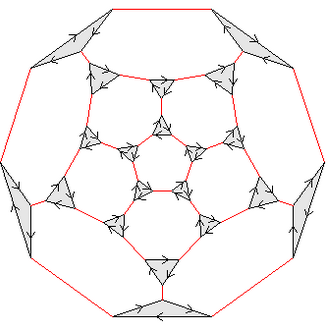
\includegraphics[width=.32\textwidth]{trunc-dodecahedron.png}
    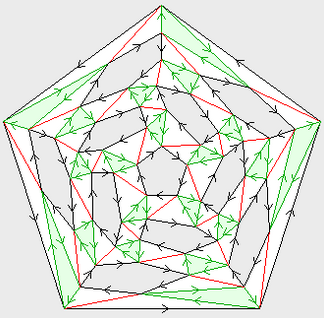
\includegraphics[width=.32\textwidth]{snub-dodecahedron.png}
    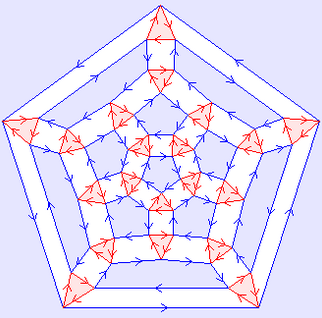
\includegraphics[width=.32\textwidth]{small-rhombicosidodec.png}
  \end{center}
  
  \begin{center}
      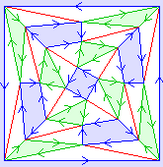
\includegraphics[width=.32\textwidth]{snub-cube.png}
      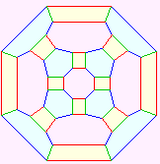
\includegraphics[width=.32\textwidth]{trunc-cuboctahedron.png}
      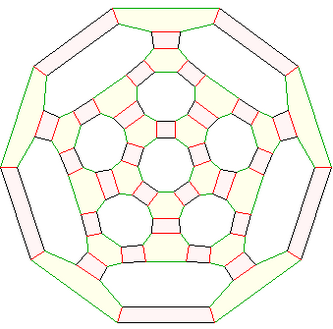
\includegraphics[width=.32\textwidth]{great-rhombicosidodec.png}
  \end{center}

\end{frame}

%%====================================================================

\begin{frame}{Symmetry groups of Platonic solids} %\Pause
  
  Two-dimensional regular polytopes have rotation groups ($C_n$) and
  symmetry groups ($D_n$). \medskip\Pause
  
  3D regular polytopes (Platonic solids) have these as well.  \medskip\Pause

  \begin{center}
  \begin{tabular}{|l|c|c|} \hline
    \textbf{solid} & \textbf{rotation group} & \textbf{symmetry group} \\
    \hline
    Tetrahedron & $A_4$ & $S_4$ \\ \hline
    Cube & $S_4$ & $S_4\times C_2$ \\
    Octahedron & $S_4$ & $S_4\times C_2$ \\ \hline
    Icosahedron & $A_5$ & $A_5\times C_2$ \\
    Dodecahedron & $A_5$ & $A_5\times C_2$ \\ \hline
  \end{tabular}
  \end{center}

  \vspace{-3mm}
  
  \begin{center}
    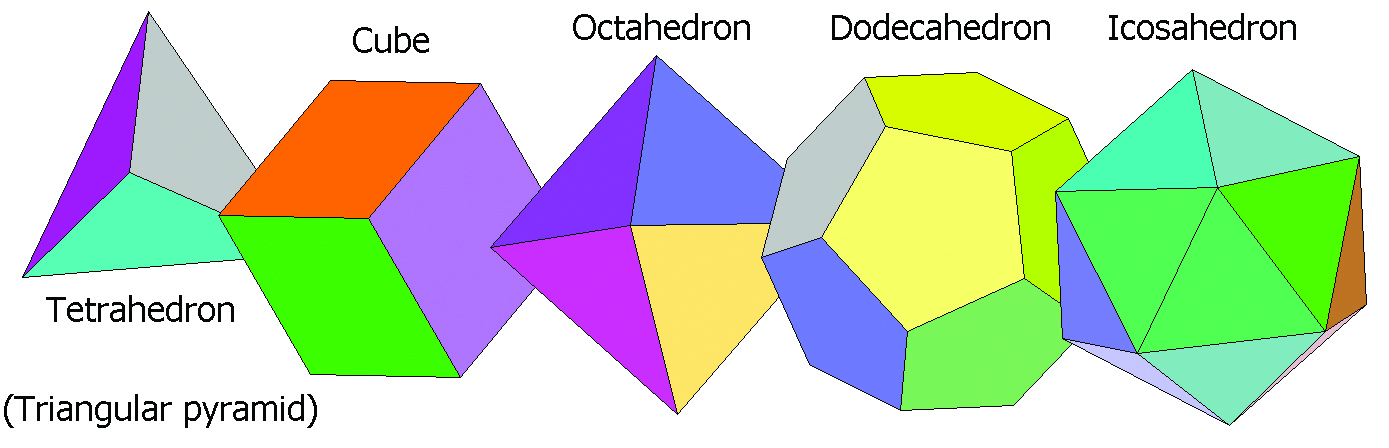
\includegraphics[width=.7\textwidth]{platonic-solids}
  \end{center}

  \Pause
  
  There are higher-dimensional versions of the tetrahedron and cube,
  and their symmetry groups are $S_n$, and a group we haven't yet seen
  called $S_n\wr C_2$ (the ``\Balert{signed permutations}'').
  
\end{frame}

%%====================================================================
%%====================================================================

\begin{frame}{Generalizing the quaternion group} \smallskip

  The \textbf{quaternion group} $Q_8$ is generated by:
  \begin{itemize}
  \item a \Alert{$4^{\rm th}$ root of unity}, $i=\zeta_4=e^{2\pi i/4}$
    ($2\pi/4$-rotation)
  \item the ``\Balert{imaginary number}'' $j$
  \end{itemize}
  \[
  Q_8\!=\!\big\<\Alert{i},\Balert{j},k\big\>\cong\left\<
  \underbrace{\Alert{\begin{bmatrix} i & 0 \\ 0 & -i\end{bmatrix}}}_{R=R_4},
  \underbrace{\Balert{\begin{bmatrix} 0 & 1 \\ -1 & 0\end{bmatrix}}}_{S},
  \underbrace{\begin{bmatrix} 0 & i \\ i & 0\end{bmatrix}}_{T=RS}\right\>.
  \]
  The \textbf{dihedral group} is generated by 
  \begin{itemize}
  \item an \Alert{$n^{\rm th}$ root of unity}, $r=\zeta_n=e^{2\pi i/n}$
    ($2\pi/n$-rotation)
  \item a \Balert{reflection} $f$
  \end{itemize}
  
  \vspace{-7mm}
  
  \[
  D_n\!=\!\<\Alert{r},\Balert{f}\>\!\cong\!\left\<\underbrace{\Alert{
      \begin{bmatrix}\zeta_n & 0
        \\ 0 & \overline{\zeta}_n\end{bmatrix}}}_{R_n},
  \Balert{\underbrace{\begin{bmatrix}0 & 1 \\ 1 & 0\end{bmatrix}}_{\Balert{F}}}
  \right\>\!.
  \]
  
  \vspace{-3mm}
  
  %% Cayley graph of Q8 and D6
  \[
  \begin{tikzpicture}[scale=.7]
    \tikzstyle{v} = [circle, draw, fill=lightgray,inner sep=0pt,
      minimum size=3.5mm]
    \tikzstyle{R6-out} = [draw, very thick, eRed,-stealth,bend right=18]
    \tikzstyle{R6-in} = [draw, very thick, eRed,-stealth,bend left=12]
    \tikzstyle{R-out} = [draw, very thick, eRed,-stealth,bend right=15]
    \tikzstyle{R-in} = [draw, very thick, eRed,-stealth,bend left=12]
    \tikzstyle{B} = [draw, very thick, eBlue,-stealth,bend right=25]
    %%
    %% Cayley graph of Q8=<r,s>
    %%
    \begin{scope}[shift={(0,0)},scale=.95]
      \tikzstyle{every node}=[font=\scriptsize]
      \node (1) at (0:2) [v] {$1$};
      \node (r) at (90:2) [v] {$i$};
      \node (r2) at (180:2) [v] {$-1$};
      \node (r3) at (270:2) [v] {$-i$};
      \node (s) at (0:1) [v] {$j$};
      \node (sr) at (270:1) [v] {$-k$};
      \node (sr2) at (180:1) [v] {$-j$};
      \node (sr3) at (90:1) [v] {$k$};
      %%
      \draw [b] (1) to (s); \draw [B] (s) to (r2);
      \draw [b] (r2) to (sr2); \draw [B] (sr2) to (1);
      %%
      \draw [b] (r) to (sr3); \draw [B] (sr3) to (r3);
      \draw [b] (r3) to (sr); \draw [B] (sr) to (r);
      %%
      \draw [r] (1) to [bend right] (r);
      \draw [r] (r) to [bend right] (r2);
      \draw [r] (r2) to [bend right] (r3);
      \draw [r] (r3) to [bend right] (1);
      \draw [r] (s) to [bend left=28] (sr);
      \draw [r] (sr) to [bend left=28] (sr2);
      \draw [r] (sr2) to [bend left=28] (sr3);
      \draw [r] (sr3) to [bend left=28] (s);
      %%
      \node at (0,0) {\normalsize $Q_8$};
    \end{scope}
    %%
    %% Cayley graph of D6=<r,f>
    %%
    \begin{scope}[shift={(7,0)},scale=1]
      \tikzstyle{every node}=[font=\scriptsize]
      \node (1) at (0:2) [v] {$1$};
      \node (r) at (60:2) [v] {$r$};
      \node (r2) at (120:2) [v] {$r^2$};
      \node (r3) at (180:2) [v] {$r^3$};
      \node (r4) at (240:2) [v] {$r^4$};
      \node (r5) at (300:2) [v] {$r^5$};
      \node (s) at (0:1) [v] {$f$};
      \node (sr5) at (60:1) [v] {$rf$};
      \node (sr4) at (120:1) [v] {$r^2\!f$};
      \node (sr3) at (180:1) [v] {$r^3\!f$};
      \node (sr2) at (240:1) [v] {$r^4\!f$};
      \node (sr) at (300:1) [v] {$r^5\!f$};
      \path[bb] (1) to (s);
      \path[bb] (r) to (sr5);
      \path[bb] (r2) to (sr4);
      \path[bb] (r3) to (sr3);
      \path[bb] (r4) to (sr2);
      \path[bb] (r5) to (sr);
      \path[R-out] (1) to (r);
      \path[R6-out] (r) to (r2);
      \path[R6-out] (r2) to (r3);
      \path[R6-out] (r3) to (r4);
      \path[R6-out] (r4) to (r5);
      \path[R6-out] (r5) to (1);
      \path[R-in] (sr5) to (s);
      \path[R-in] (sr4) to (sr5);
      \path[R-in] (sr3) to (sr4);
      \path[R-in] (sr2) to (sr3);
      \path[R-in] (sr) to (sr2);
      \path[R-in] (s) to (sr);
      \node at (0,0) {\normalsize $D_6$};
    \end{scope}
  \end{tikzpicture}
  \]  
  
\end{frame}

%%====================================================================

\begin{frame}{The dicyclic groups} \smallskip
  
  When $n$ is even, we can replace $\zeta_4$ with $\zeta_n$ to get the \textbf{dicyclic group}
  \[
  \Dic_n=\big\<\zeta_n,j\big\>\cong\left\<\Alert{\begin{bmatrix}\zeta_n & 0 \\
      0 & \overline{\zeta}_n\end{bmatrix}},\;
  \Balert{\begin{bmatrix}0 & 1 \\ -1 & 0\end{bmatrix}}\right\>
  \cong\big\<r,s\mid r^n=s^4=1,\;r^{n/2}=s^2,\;rsr=s\big\>. 
  \]
  \emph{The multiplication rules $ij=k$ and $ji=-k$ remain unchanged.}

  \Pause

  %% Two Cayley graphs of Dic6
  \[
  \begin{tikzpicture}[scale=1.25,baseline=1.3ex,auto]
    \tikzstyle{R-out} = [draw, very thick, eRed,-stealth,bend right=17]
    \tikzstyle{R-in} = [draw, very thick, eRed,-stealth,bend left=12]
    \tikzstyle{B} = [draw, very thick, eBlue,-stealth,bend left=28]
    \tikzstyle{every node}=[font=\tiny]
    %%
    %% Cayley graph of Dic6 with nodes labeled by complex numbers.
    %% 
    \begin{scope}[shift={(0,0)},scale=1]
      \tikzstyle{v} = [circle,fill=lightgray,draw,inner sep=0pt,
        minimum size=7.5mm]
      \node (1) at (0:2.0) [v] {\footnotesize $1$};
      \node (r) at (60:2.0) [v] {$\frac{1}{2}\!\!+\!\!\frac{\sqrt{3}}{2}\!i$};
      \node (r2) at (120:2.0) [v] {$-\!\frac{1}{2}\!\!
        +\!\!\frac{\sqrt{3}}{2}\!i$};
      \node (r3) at (180:2.0) [v] {\footnotesize $-1$};
      \node (r4) at (240:2.0) [v] {$-\!\frac{1}{2}\!\!
        -\!\!\frac{\sqrt{3}}{2}\!i$};
      \node (r5) at (300:2.0) [v] {$\frac{1}{2}\!\!-\!\!\frac{\sqrt{3}}{2}\!i$};
      \node (s) at (0:1) [v] {\footnotesize $j$};
      \node (sr5) at (60:1) [v] {$\!\frac{1}{2}j\!\!
        +\!\!\frac{\sqrt{3}}{2}\!k$};
      \node (sr4) at (120:1) [v] {$-\!\frac{1}{2}j\!\!
        +\!\!\frac{\sqrt{3}}{2}\!k$};
      \node (sr3) at (180:1) [v] {\footnotesize $-j$};
      \node (sr2) at (240:1) [v] {$-\frac{1}{2}j\!\!
        -\!\!\frac{\sqrt{3}}{2}\!k$};
      \node (sr) at (300:1) [v] {$\frac{1}{2}j\!\!
        -\!\!\frac{\sqrt{3}}{2}\!k$};
      \path[b] (1) to (s);
      \path[B] (s) to (r3);
      \path[b] (r3) to (sr3);
      \path[B] (sr3) to (1);
      %%
      \path[b] (r) to (sr5);
      \path[B] (sr5) to (r4);
      \path[b] (r4) to (sr2);
      \path[B] (sr2) to (r);
      %%
      \path[b] (r2) to (sr4);
      \path[B] (sr4) to (r5);
      \path[b] (r5) to (sr);
      \path[B] (sr) to (r2);
      %%
      \path[R-out] (1) to (r);
      \path[R-out] (r) to (r2);
      \path[R-out] (r2) to (r3);
      \path[R-out] (r3) to (r4);
      \path[R-out] (r4) to (r5);
      \path[R-out] (r5) to (1);
      \path[R-in] (sr5) to (s);
      \path[R-in] (sr4) to (sr5);
      \path[R-in] (sr3) to (sr4);
      \path[R-in] (sr2) to (sr3);
      \path[R-in] (sr) to (sr2);
      \path[R-in] (s) to (sr);
      %%
      \node at (0,0) {\normalsize $\Dic_6$};
    \end{scope}   
    %%
    %% Cayley graph of Dic_6 with nodes labeled by \zeta and j.
    %% 
    \begin{scope}[shift={(5,0)},scale=.65]
      \tikzstyle{every node}=[font=\footnotesize]
      \node at (0,0) {\normalsize $\Dic_6$};
      \node[v] (1) at (0:3) {$1$}; 
      \node[v] (r) at (0:2) {$\zeta$};
      \node[v] (r2) at (0:1) {$\zeta^2$};
      %%
      \node[v] (s) at (90:3) {$j$};
      \node[v] (rs) at (90:2) {$\zeta\,j$};
      \node[v] (r2s) at (90:1) {$\zeta^2\!j$};
      %%
      \node[v] (s2) at (180:3) {$-1$};
      \node[v] (rs2) at (180:2) {$-\!\zeta$};
      \node[v] (r2s2) at (180:1) {\scriptsize$-\!\zeta^2$};
      %%
      \node[v] (s3) at (-90:3) {$-j$};
      \node[v] (rs3) at (-90:2) {\scriptsize $-\zeta j$};
      \node[v] (r2s3) at (-90:1) {\scriptsize $-\zeta^2\!j$};
      %%
      \draw[r] (1) to (r);
      \draw[r] (r) to (r2);
      %%
      \draw[r] (s2) to (rs2);
      \draw[r] (rs2) to (r2s2);
      %%
      \draw[r] (r2s) to (rs);
      \draw[r] (rs) to (s);
      %%
      \draw[r] (r2s3) to (rs3);
      \draw[r] (rs3) to (s3);
      %%
      \draw[r,bend right=28] (r2) to (s2); 
      \draw[r,bend right=28] (r2s2) to (1); 
      \draw[r,bend right=28] (s) to (r2s3); 
      \draw[r,bend right=28] (s3) to (r2s); 
      %%
      \draw[b,bend right=28] (1) to (s);
      \draw[b,bend right=28] (r) to (rs);
      \draw[b,bend right=28] (r2) to (r2s);
      %%
      \draw[b,bend right=28] (s) to (s2);
      \draw[b,bend right=28] (rs) to (rs2);
      \draw[b,bend right=28] (r2s) to (r2s2);
      %%
      \draw[b,bend right=28] (s2) to (s3);
      \draw[b,bend right=28] (rs2) to (rs3);
      \draw[b,bend right=28] (r2s2) to (r2s3);
      %%
      \draw[b,bend right=28] (s3) to (1);
      \draw[b,bend right=28] (rs3) to (r);
      \draw[b,bend right=28] (r2s3) to (r2);
    \end{scope}
  \end{tikzpicture}
  \]
  
\end{frame}

%%====================================================================

\begin{frame}{The dicyclic groups} \vspace{-8mm}
  
  %% Cayley graphs of Dic_n (n=4, 6, 8) with blue 4-cycles
  %% 
  \[
  \begin{tikzpicture}[scale=.55]
    \tikzstyle{v} = [circle, draw, fill=lightgray,inner sep=0pt, 
      minimum size=3.5mm]
    \tikzstyle{v-r} = [circle, draw, fill=vRed,inner sep=0pt,
      minimum size=3.5mm]
    \tikzstyle{v-b} = [circle, draw, fill=vBlue,inner sep=0pt,
      minimum size=3.5mm]
    \tikzstyle{v-p} = [circle, draw, fill=vPurple,inner sep=0pt, 
      minimum size=3.5mm]
    \tikzstyle{every node}=[font=\tiny]
    %%
    %% Cayley graph of Dic4 (blue circles)
    %% 
    \begin{scope}[shift={(0,0)}]
      \node[v-p] (1) at (0:2) {$1$};
      \node[v-r] (r) at (0:1) {$r$};
      %%
      \node[v-b] (s) at (90:2) {$s$};
      \node[v] (rs) at (90:1) {$rs$};
      %%
      \node[v-p] (s2) at (180:2) {$s^2$};
      \node[v-r] (rs2) at (180:1) {$rs^2$};
      %%
      \node[v-b] (s3) at (-90:2) {$s^3$};
      \node[v] (rs3) at (-90:1) {$rs^3$};
      %
      \draw[r] (1) to (r);
      \draw[r] (s2) to (rs2);
      \draw[r] (rs) to (s);
      \draw[r] (rs3) to (s3);
      %%
      \draw[r,bend right=28] (r) to (s2); 
      \draw[r,bend right=28] (rs2) to (1); 
      \draw[r,bend right=28] (s) to (rs3); 
      \draw[r,bend right=28] (s3) to (rs); 
      %%
      \draw[b,bend right=20] (1) to (s);
      \draw[b,bend right=20] (r) to (rs);
      %%
      \draw[b,bend right=20] (s) to (s2);
      \draw[b,bend right=20] (rs) to (rs2);
      %%
      \draw[b,bend right=20] (s2) to (s3);
      \draw[b,bend right=20] (rs2) to (rs3);
      %%
      \draw[b,bend right=20] (s3) to (1);
      \draw[b,bend right=20] (rs3) to (r);
    \end{scope}
    %%
    %% Cayley graph of Dic6 (blue circles)
    %% 
    \begin{scope}[shift={(6.5,0)}]
      \node[v-p] (1) at (0:3) {$1$};
      \node[v-r] (r) at (0:2) {$r$};
      \node[v-r] (r2) at (0:1) {$r^2$};
      %%
      \node[v-b] (s) at (90:3) {$s$};
      \node[v] (rs) at (90:2) {$rs$};
      \node[v] (r2s) at (90:1) {$r^2\!s$};
      %%
      \node[v-p] (s2) at (180:3) {$s^2$};
      \node[v-r] (rs2) at (180:2) {$rs^2$};
      \node[v-r] (r2s2) at (180:1) {$r^2\!\!s^2$};
      %%
      \node[v-b] (s3) at (-90:3) {$s^3$};
      \node[v] (rs3) at (-90:2) {$rs^3$};
      \node[v] (r2s3) at (-90:1) {$r^2\!\!s^3$};
      %%
      \draw[r] (1) to (r);
      \draw[r] (r) to (r2);
      %%
      \draw[r] (s2) to (rs2);
      \draw[r] (rs2) to (r2s2);
      %%
      \draw[r] (r2s) to (rs);
      \draw[r] (rs) to (s);
      %%
      \draw[r] (r2s3) to (rs3);
      \draw[r] (rs3) to (s3);
      %%
      \draw[r,bend right=28] (r2) to (s2); 
      \draw[r,bend right=28] (r2s2) to (1); 
      \draw[r,bend right=28] (s) to (r2s3); 
      \draw[r,bend right=28] (s3) to (r2s); 
      %%
      \draw[b,bend right=20] (1) to (s);
      \draw[b,bend right=20] (r) to (rs);
      \draw[b,bend right=20] (r2) to (r2s);
      %%
      \draw[b,bend right=20] (s) to (s2);
      \draw[b,bend right=20] (rs) to (rs2);
      \draw[b,bend right=20] (r2s) to (r2s2);
      %%
      \draw[b,bend right=20] (s2) to (s3);
      \draw[b,bend right=20] (rs2) to (rs3);
      \draw[b,bend right=20] (r2s2) to (r2s3);
      %%
      \draw[b,bend right=20] (s3) to (1);
      \draw[b,bend right=20] (rs3) to (r);
      \draw[b,bend right=20] (r2s3) to (r2);
  \end{scope}
    %%
    %% Cayley graph of Dic8 (blue circles)
    %% 
    \begin{scope}[shift={(15,0)}]
          \node[v-p] (1) at (0:4) {$1$};
      \node[v-r] (r) at (0:3) {$r$};
      \node[v-r] (r2) at (0:2) {$r^2$};
      \node[v-r] (r3) at (0:1) {$r^3$};
      %%
      \node[v-b] (s) at (90:4) {$s$};
      \node[v] (rs) at (90:3) {$rs$};
      \node[v] (r2s) at (90:2) {$r^2\!s$};
      \node[v] (r3s) at (90:1) {$r^3\!s$};
      %%
      \node[v-p] (s2) at (180:4) {$s^2$};
      \node[v-r] (rs2) at (180:3) {$rs^2$};
      \node[v-r] (r2s2) at (180:2) {$r^2\!\!s^2$};
      \node[v-r] (r3s2) at (180:1) {$r^3\!\!s^2$};
      %%
      \node[v-b] (s3) at (-90:4) {$s^3$};
      \node[v] (rs3) at (-90:3) {$rs^3$};
      \node[v] (r2s3) at (-90:2) {$r^2\!\!s^3$};
      \node[v] (r3s3) at (-90:1) {$r^3\!\!s^3$};
      %%
      \draw[r] (1) to (r);
      \draw[r] (r) to (r2);
      \draw[r] (r2) to (r3);
      %%
      \draw[r] (s2) to (rs2);
      \draw[r] (rs2) to (r2s2);
      \draw[r] (r2s2) to (r3s2);
      %%
      \draw[r] (r3s) to (r2s);
      \draw[r] (r2s) to (rs);
      \draw[r] (rs) to (s);
      %%
      \draw[r] (r3s3) to (r2s3);
      \draw[r] (r2s3) to (rs3);
      \draw[r] (rs3) to (s3);
      %%
      \draw[r,bend right=28] (r3) to (s2); 
      \draw[r,bend right=28] (r3s2) to (1); 
      \draw[r,bend right=28] (s) to (r3s3); 
      \draw[r,bend right=28] (s3) to (r3s); 
      %%
      \draw[b,bend right=20] (1) to (s);
      \draw[b,bend right=20] (r) to (rs);
      \draw[b,bend right=20] (r2) to (r2s);
      \draw[b,bend right=20] (r3) to (r3s);
      %%
      \draw[b,bend right=20] (s) to (s2);
      \draw[b,bend right=20] (rs) to (rs2);
      \draw[b,bend right=20] (r2s) to (r2s2);
      \draw[b,bend right=20] (r3s) to (r3s2);
      %%
      \draw[b,bend right=20] (s2) to (s3);
      \draw[b,bend right=20] (rs2) to (rs3);
      \draw[b,bend right=20] (r2s2) to (r2s3);
      \draw[b,bend right=20] (r3s2) to (r3s3);
      %%
      \draw[b,bend right=20] (s3) to (1);
      \draw[b,bend right=20] (rs3) to (r);
      \draw[b,bend right=20] (r2s3) to (r2);
      \draw[b,bend right=20] (r3s3) to (r3);
  \end{scope}      
  \end{tikzpicture}
  \]

  \vspace{-3mm}
  
  %% Cycle graphs of Dic_n (n=4, 6, 8)
  \[
  \begin{tikzpicture}[scale=.45,auto]
    \tikzstyle{v} = [circle, draw, fill=lightgray,inner sep=0pt,
      minimum size=3.5mm]
    \tikzstyle{v-r} = [circle, draw, fill=vRed,inner sep=0pt,
      minimum size=3.5mm]
    \tikzstyle{v-b} = [circle, draw, fill=vBlue,inner sep=0pt,
      minimum size=3.5mm]
    \tikzstyle{v-p} = [circle, draw, fill=vPurple,inner sep=0pt, 
      minimum size=3.5mm]
    \tikzstyle{cy2-r} = [draw]
    \tikzstyle{cy2-s} = [draw,eBlue]
    \tikzstyle{cy2-rs} = [draw,ePurple]
    \tikzstyle{cy2-r2s} = [draw,eGreen]
    \tikzstyle{cy2-r3s} = [draw,eOrange] 
    \tikzstyle{every node}=[font=\tiny]
    %%
    %% Cycle graph for Dic4
    %%
    \begin{scope}[shift={(0,0)}]
      \node (-i) at (-.5,0) [v-r] {$-\!i$};
      \node (i) at (.5,0) [v-r] {$i$};
      \node (-j) at (-1.5,0) [v-b] {$-\!j$};
      \node (j) at (1.5,0) [v-b] {$j$};
      \node (-k) at (-2.5,0) [v] {$-\!k$};
      \node (k) at (2.5,0) [v] {$k$};
      \node (1) at (0,3) [v-p] {$1$};
      \node (-1) at (0,-3) [v-p] {$-1$};
      \draw [cy2-r] (1) to (i); \draw [cy2-r] (1) to (-i);
      \draw [cy2-s] (1) to (j); \draw [cy2-s] (1) to (-j);
      \draw [cy2-rs] (1) to (k); \draw [cy2-rs] (1) to (-k);
      \draw [cy2-r] (-1) to (i); \draw [cy2-r] (-1) to (-i);
      \draw [cy2-s] (-1) to (j); \draw [cy2-s] (-1) to (-j);
      \draw [cy2-rs] (-1) to (k); \draw [cy2-rs] (-1) to (-k);
    \end{scope}
    %%
    %% Cycle graph for Dic6
    %%
    \begin{scope}[shift={(8,0)}]
      \node (1) at (0,3) [v-p] {$1$};
      \node (s2) at (0,-3) [v-p] {$s^2$};
      \node (r) at (.5,1) [v-r] {$r$};
      \node (r2) at (.5,-1) [v-r] {$r^2$};
      \node (rs2) at (-.5,-1) [v-r] {$r^4$};
      \node (r2s2) at (-.5,1) [v-r] {$r^5$};
      %%
      \node (s3) at (-1.5,0) [v-b] {$s^3$};
      \node (s) at (1.5,0) [v-b] {$s$};
      \node (rs3) at (-2.5,0) [v] {$rs^3$};
      \node (rs) at (2.5,0) [v] {$rs$};
      \node (r2s3) at (-3.5,0) [v] {$r^2\!s^3$};
      \node (r2s) at (3.5,0) [v] {$r^2\!s$};
      %%
      \draw [cy2-r] (1) to (r);
      \draw [cy2-r] (r) to (r2);
      \draw [cy2-r] (r2) to (s2);
      \draw [cy2-r] (s2) to (rs2);
      \draw [cy2-r] (rs2) to (r2s2);
      \draw [cy2-r] (r2s2) to (1);
      %%
      \draw [cy2-s,bend left=10] (1) to (s);
      \draw [cy2-s,bend right=10] (s2) to (s);
      \draw [cy2-rs,bend left=5] (1) to (rs);
      \draw [cy2-rs,bend right=5] (s2) to (rs);
      \draw [cy2-r2s] (1) to (r2s); \draw [cy2-r2s] (s2) to (r2s);
      \draw [cy2-s, bend right=10] (1) to (s3);
      \draw [cy2-s,bend left=10] (s2) to (s3);
      \draw [cy2-rs,bend right=5] (1) to (rs3);
      \draw [cy2-rs,bend left=5] (s2) to (rs3);
      \draw [cy2-r2s] (1) to (r2s3); \draw [cy2-r2s] (s2) to (r2s3);
    \end{scope}
    %%
    %% Cycle graph for Dic8
    %%
    \begin{scope}[shift={(18,0)}]
      \node (1) at (0,3) [v-p] {$1$};
      \node (s2) at (0,-3) [v-p] {$s^2$};
      %%
      \node (s3) at (-1.5,0) [v-b] {$s^3$};
      \node (s) at (1.5,0) [v-b] {$s$};
      \node (rs3) at (-2.5,0) [v] {$rs^3$};
      \node (rs) at (2.5,0) [v] {$rs$};
      \node (r2s3) at (-3.5,0) [v] {$r^2\!s^3$};
      \node (r2s) at (3.5,0) [v] {$r^2\!s$};
      \node (r3s3) at (-4.5,0) [v] {$r^3\!s^3$};
      \node (r3s) at (4.5,0) [v] {$r^3\!s$};
      %%
      \draw [cy2-s,bend left=17] (1) to (s);
      \draw [cy2-s,bend right=17] (s2) to (s);
      \draw [cy2-rs,bend left=10] (1) to (rs);
      \draw [cy2-rs,bend right=10] (s2) to (rs);
      \draw [cy2-r2s,bend left=5] (1) to (r2s);
      \draw [cy2-r2s,bend right=5] (s2) to (r2s);
      \draw [cy2-r3s] (1) to (r3s); \draw [cy2-r3s] (s2) to (r3s);
      \draw [cy2-s,bend right=17] (1) to (s3);
      \draw [cy2-s,bend left=17] (s2) to (s3);
      \draw [cy2-rs,bend right=10] (1) to (rs3);
      \draw [cy2-rs,bend left=10] (s2) to (rs3);
      \draw [cy2-r2s,bend right=5] (1) to (r2s3);
      \draw [cy2-r2s,bend left=5] (s2) to (r2s3);
      \draw [cy2-r3s] (1) to (r3s3); \draw [cy2-r3s] (s2) to (r3s3);
      %%
      \node (r) at (.5,1.5) [v-r] {$r$};
      \node (r2) at (.5,0) [v-r] {$r^2$};
      \node (r3) at (.5,-1.5) [v-r] {$r^3$};
      \node (rs2) at (-.5,-1.5) [v-r] {$r^5$};
      \node (r2s2) at (-.5,0) [v-r] {$r^6$};
      \node (r3s2) at (-.5,1.5) [v-r] {$r^7$};
      %%
      \draw [cy2-r] (1) to (r);
      \draw [cy2-r] (r) to (r2);
      \draw [cy2-r] (r2) to (r3);
      \draw [cy2-r] (r3) to (s2);
      \draw [cy2-r] (s2) to (rs2);
      \draw [cy2-r] (rs2) to (r2s2);
      \draw [cy2-r] (r2s2) to (r3s2);
      \draw [cy2-r] (r3s2) to (1);
    \end{scope}
  \end{tikzpicture}
  \]
  
\end{frame}

%%====================================================================

\begin{frame}{A quotient of the dicyclic group $\Dic_4$} \smallskip

  The quaternion group is $Q_8=\<\zeta_4,j\>=\{\pm 1,\pm i,\pm j,\pm
  k\}=\Dic_4$.

  \medskip
  
  Recall how we constructed a \Balert{quotient} of $Q_8$, which was
  \[
  Q_8/\<-1\>\cong V_4.
  \]

  \vspace{-2mm}
  
  \[
  \newcommand*{\n}{9}%
  \begin{tikzpicture}[scale=.7]
        \begin{scope}[shift={(0,0)},scale=1.5]
      \tikzstyle{every node}=[font=\small]
      \node (1) at (135:1) [v] {$1$};
      \node (i) at (45:1) [v] {$i$};
      \node (k) at (-45:1) [v] {$k$};
      \node (j) at (-135:1) [v] {$j$};
      \node (-1) at (135:2) [v] {$-1$};
      \node (-i) at (45:2) [v] {$-i$};
      \node (-k) at (-45:2) [v] {$-k$};
      \node (-j) at (-135:2) [v] {$-j$};
      \node at (0,0) {\normalsize $Q_8$};
      %%
      \path[r] (1) to (i);
      \path[r] (i) to (-1);
      \path[r] (-1) to (-i);
      \path[r] (-i) to (1);
      %%
      \path[r] (k) to (j);
      \path[r] (j) to (-k);
      \path[r] (-k) to (-j);
      \path[r] (-j) to (k);
      %%
      \path[b] (i) to (k);
      \path[b] (k) to (-i);
      \path[b] (-i) to (-k);
      \path[b] (-k) to (i);
      %%
      \path[b] (1) to (j);
      \path[b] (j) to (-1);
      \path[b] (-1) to (-j);
      \path[b] (-j) to (1);
      %%
      \path[gg] (1) to (-1);
      \path[gg] (j) to (-j);
      \path[gg] (i) to (-i);
      \path[gg] (k) to (-k);
    \end{scope}
    %%
    \colorlet{color_1}{tGreen}
    \colorlet{color_-1}{tGreen}
    \colorlet{color_i}{tRed}
    \colorlet{color_-i}{tRed}
    \colorlet{color_j}{tBlue}
    \colorlet{color_-j}{tBlue}
    \colorlet{color_k}{tYellow}
    \colorlet{color_-k}{tYellow}
    \begin{scope}[scale=.6,shift={(6.5,-5.5)}]
      \tikzstyle{every node}=[font=\footnotesize]
      %% Left column of table (header)
      \path[fill=color_1] (-.1,8) rectangle ++(1,1);
      \path[fill=color_-1] (-.1,7) rectangle ++(1,1);
      \path[fill=color_i] (-.1,6) rectangle ++(1,1);
      \path[fill=color_-i] (-.1,5) rectangle ++(1,1);
      \path[fill=color_j] (-.1,4) rectangle ++(1,1);
      \path[fill=color_-j] (-.1,3) rectangle ++(1,1);
      \path[fill=color_k] (-.1,2) rectangle ++(1,1);
      \path[fill=color_-k] (-.1,1) rectangle ++(1,1);
      %% Top row of table (header)
      \path[fill=color_1] (1,9.1) rectangle ++(1,1);
      \path[fill=color_-1] (2,9.1) rectangle ++(1,1);
      \path[fill=color_i] (3,9.1) rectangle ++(1,1);
      \path[fill=color_-i] (4,9.1) rectangle ++(1,1);
      \path[fill=color_j] (5,9.1) rectangle ++(1,1);
      \path[fill=color_-j] (6,9.1) rectangle ++(1,1);
      \path[fill=color_k] (7,9.1) rectangle ++(1,1);
      \path[fill=color_-k] (8,9.1) rectangle ++(1,1);
      % Top row of table
      \path[fill=color_1] (1,8) rectangle ++(1,1);
      \path[fill=color_-1] (2,8) rectangle ++(1,1);
      \path[fill=color_i] (3,8) rectangle ++(1,1);
      \path[fill=color_-i] (4,8) rectangle ++(1,1);
      \path[fill=color_j] (5,8) rectangle ++(1,1);
      \path[fill=color_-j] (6,8) rectangle ++(1,1);
      \path[fill=color_k] (7,8) rectangle ++(1,1);
      \path[fill=color_-k] (8,8) rectangle ++(1,1);
      %
      \path[fill=color_-1] (1,7) rectangle ++(1,1);
      \path[fill=color_1] (2,7) rectangle ++(1,1);
      \path[fill=color_-i] (3,7) rectangle ++(1,1);
      \path[fill=color_i] (4,7) rectangle ++(1,1);
      \path[fill=color_-j] (5,7) rectangle ++(1,1);
      \path[fill=color_j] (6,7) rectangle ++(1,1);
      \path[fill=color_-k] (7,7) rectangle ++(1,1);
      \path[fill=color_k] (8,7) rectangle ++(1,1);
      %
      \path[fill=color_i] (1,6) rectangle ++(1,1);
      \path[fill=color_-i] (2,6) rectangle ++(1,1);
      \path[fill=color_-1] (3,6) rectangle ++(1,1);
      \path[fill=color_1] (4,6) rectangle ++(1,1);
      \path[fill=color_k] (5,6) rectangle ++(1,1);
      \path[fill=color_-k] (6,6) rectangle ++(1,1);
      \path[fill=color_-j] (7,6) rectangle ++(1,1);
      \path[fill=color_j] (8,6) rectangle ++(1,1);
      %
      \path[fill=color_-i] (1,5) rectangle ++(1,1);
      \path[fill=color_i] (2,5) rectangle ++(1,1);
      \path[fill=color_1] (3,5) rectangle ++(1,1);
      \path[fill=color_-1] (4,5) rectangle ++(1,1);
      \path[fill=color_-k] (5,5) rectangle ++(1,1);
      \path[fill=color_k] (6,5) rectangle ++(1,1);
      \path[fill=color_j] (7,5) rectangle ++(1,1);
      \path[fill=color_-j] (8,5) rectangle ++(1,1);
      %
      \path[fill=color_j] (1,4) rectangle ++(1,1);
      \path[fill=color_-j] (2,4) rectangle ++(1,1);
      \path[fill=color_-k] (3,4) rectangle ++(1,1);
      \path[fill=color_k] (4,4) rectangle ++(1,1);
      \path[fill=color_-1] (5,4) rectangle ++(1,1);
      \path[fill=color_1] (6,4) rectangle ++(1,1);
      \path[fill=color_i] (7,4) rectangle ++(1,1);
      \path[fill=color_-i] (8,4) rectangle ++(1,1);
      %
      \path[fill=color_-j] (1,3) rectangle ++(1,1);
      \path[fill=color_j] (2,3) rectangle ++(1,1);
      \path[fill=color_k] (3,3) rectangle ++(1,1);
      \path[fill=color_-k] (4,3) rectangle ++(1,1);
      \path[fill=color_1] (5,3) rectangle ++(1,1);
      \path[fill=color_-1] (6,3) rectangle ++(1,1);
      \path[fill=color_-i] (7,3) rectangle ++(1,1);
      \path[fill=color_i] (8,3) rectangle ++(1,1);
      %
      \path[fill=color_k] (1,2) rectangle ++(1,1);
      \path[fill=color_-k] (2,2) rectangle ++(1,1);
      \path[fill=color_j] (3,2) rectangle ++(1,1);
      \path[fill=color_-j] (4,2) rectangle ++(1,1);
      \path[fill=color_-i] (5,2) rectangle ++(1,1);
      \path[fill=color_i] (6,2) rectangle ++(1,1);
      \path[fill=color_-1] (7,2) rectangle ++(1,1);
      \path[fill=color_1] (8,2) rectangle ++(1,1);
      %
      \path[fill=color_-k] (1,1) rectangle ++(1,1);
      \path[fill=color_k] (2,1) rectangle ++(1,1);
      \path[fill=color_-j] (3,1) rectangle ++(1,1);
      \path[fill=color_j] (4,1) rectangle ++(1,1);
      \path[fill=color_i] (5,1) rectangle ++(1,1);
      \path[fill=color_-i] (6,1) rectangle ++(1,1);
      \path[fill=color_1] (7,1) rectangle ++(1,1);
      \path[fill=color_-1] (8,1) rectangle ++(1,1);
      %%
      \foreach \i in {1,...,\n} {
        \draw [very thin] (\i,1) -- (\i,\n); 
        \draw [very thin] (\i,\n+.1) -- (\i,\n+1.1); 
        \draw [very thin] (1,\i) -- (\n,\i); 
        \draw [very thin] (-.1,\i) -- (.9,\i); 
      }
      \draw [very thin] (1,\n+.1) rectangle (\n,\n+1.1);
      \draw [very thin] (-.1,1) rectangle (.9,\n);
      %%
      \node at (0.4,8.5) {$1$};
      \node at (0.4,7.5) {$-1$};
      \node at (0.4,6.5) {$i$};
      \node at (0.4,5.5) {$-i$}; 
      \node at (0.4,4.5) {$j$}; 
      \node at (0.4,3.5) {$-j$};
      \node at (0.4,2.5) {$k$};
      \node at (0.4,1.5) {$-k$};
      %% 
      \node at (1.5,9.6) {$1$};
      \node at (2.5,9.6) {$-1$};
      \node at (3.5,9.6) {$i$};
      \node at (4.5,9.6) {$-i$}; 
      \node at (5.5,9.6) {$j$}; 
      \node at (6.5,9.6) {$-j$};
      \node at (7.5,9.6) {$k$};
      \node at (8.5,9.6) {$-k$};
      %%
      \node at (1.5,8.5) {$1$};
      \node at (1.5,7.5) {$-1$};
      \node at (1.5,6.5) {$i$};
      \node at (1.5,5.5) {$-i$}; 
      \node at (1.5,4.5) {$j$}; 
      \node at (1.5,3.5) {$-j$};
      \node at (1.5,2.5) {$k$};
      \node at (1.5,1.5) {$-k$};
      %%
      \node at (2.5,8.5) {$-1$};
      \node at (2.5,7.5) {$1$};
      \node at (2.5,6.5) {$-i$};
      \node at (2.5,5.5) {$i$}; 
      \node at (2.5,4.5) {$-j$}; 
      \node at (2.5,3.5) {$j$};
      \node at (2.5,2.5) {$-k$};
      \node at (2.5,1.5) {$k$};
      %%
      \node at (3.5,8.5) {$i$};
      \node at (3.5,7.5) {$-i$};
      \node at (3.5,6.5) {$-1$};
      \node at (3.5,5.5) {$1$}; 
      \node at (3.5,4.5) {$-k$}; 
      \node at (3.5,3.5) {$k$};
      \node at (3.5,2.5) {$j$};
      \node at (3.5,1.5) {$-j$};
      %%
      \node at (4.5,8.5) {$-i$};
      \node at (4.5,7.5) {$i$};
      \node at (4.5,6.5) {$1$};
      \node at (4.5,5.5) {$-1$}; 
      \node at (4.5,4.5) {$k$}; 
      \node at (4.5,3.5) {$-k$};
      \node at (4.5,2.5) {$-j$};
      \node at (4.5,1.5) {$j$};
      %%
      \node at (5.5,8.5) {$j$};
      \node at (5.5,7.5) {$-j$};
      \node at (5.5,6.5) {$k$};
      \node at (5.5,5.5) {$-k$}; 
      \node at (5.5,4.5) {$-1$}; 
      \node at (5.5,3.5) {$1$};
      \node at (5.5,2.5) {$-i$};
      \node at (5.5,1.5) {$i$};
      %%
      \node at (6.5,8.5) {$-j$};
      \node at (6.5,7.5) {$j$};
      \node at (6.5,6.5) {$-k$};
      \node at (6.5,5.5) {$k$}; 
      \node at (6.5,4.5) {$1$}; 
      \node at (6.5,3.5) {$-1$};
      \node at (6.5,2.5) {$i$};
      \node at (6.5,1.5) {$-i$};
      %%
      \node at (7.5,8.5) {$k$};
      \node at (7.5,7.5) {$-k$};
      \node at (7.5,6.5) {$-j$};
      \node at (7.5,5.5) {$j$}; 
      \node at (7.5,4.5) {$i$}; 
      \node at (7.5,3.5) {$-i$};
      \node at (7.5,2.5) {$-1$};
      \node at (7.5,1.5) {$1$};
      %%
      \node at (8.5,8.5) {$-k$};
      \node at (8.5,7.5) {$k$};
      \node at (8.5,6.5) {$j$};
      \node at (8.5,5.5) {$-j$}; 
      \node at (8.5,4.5) {$-i$}; 
      \node at (8.5,3.5) {$i$};
      \node at (8.5,2.5) {$1$};
      \node at (8.5,1.5) {$-1$};
      %%
      \draw [very thick] (3,1) -- (3,9);
      \draw [very thick] (5,1) -- (5,9);
      \draw [very thick] (7,1) -- (7,9);
      \draw [very thick] (1,3) -- (9,3);
      \draw [very thick] (1,5) -- (9,5);
      \draw [very thick] (1,7) -- (9,7);
      \draw [very thick] (1.02,1.02) rectangle (8.98,8.98);
    \end{scope}
    %%
    %%
    \newcommand*{\m}{5}   % counter for Cayley tables
    \colorlet{color-e}{tGreen}
    \colorlet{color-v}{tRed}
    \colorlet{color-h}{tBlue}
    \colorlet{color-vh}{tYellow}
    %%
    \begin{scope}[shift={(11.75,1.1)},scale=1.5]
      \tikzstyle{every node}=[font=\footnotesize]
      \node (j) at (0,0) [v] {$\pm j$};
      \node (1) at (0,1) [v] {$\pm 1$};
      \node (k) at (1,0) [v] {$\pm k$};
      \node (i) at (1,1) [v] {$\pm i$};
      \draw [rr] (1) to (i);
      \draw [rr] (j) to (k);
      \draw [bb] (1) to (j);
      \draw [bb] (i) to (k);
      \node at (.5,.5) {\normalsize $V_4$};
    \end{scope}
    %%
    \begin{scope}[scale=.6,shift={(18,-5.5)},box/.style={anchor=south}]
      \tikzstyle{every node}=[font=\footnotesize]
      \path[fill=color-e] (-.1,4) rectangle ++(1,1);
      \path[fill=color-v] (-.1,3) rectangle ++(1,1);
      \path[fill=color-h] (-.1,2) rectangle ++(1,1);
      \path[fill=color-vh] (-.1,1) rectangle ++(1,1);
      %%
      \path[fill=color-e] (1,5.1) rectangle ++(1,1);
      \path[fill=color-v] (2,5.1) rectangle ++(1,1);
      \path[fill=color-h] (3,5.1) rectangle ++(1,1);
      \path[fill=color-vh] (4,5.1) rectangle ++(1,1);
      %%
      \path[fill=color-e] (1,4) rectangle ++(1,1);
      \path[fill=color-e] (2,3) rectangle ++(1,1);
      \path[fill=color-e] (3,2) rectangle ++(1,1);
      \path[fill=color-e] (4,1) rectangle ++(1,1);
      %%
      \path[fill=color-v] (1,3) rectangle ++(1,1);
      \path[fill=color-v] (2,4) rectangle ++(1,1);
      \path[fill=color-v] (3,1) rectangle ++(1,1);
      \path[fill=color-v] (4,2) rectangle ++(1,1);
      %%
      \path[fill=color-h] (1,2) rectangle ++(1,1);
      \path[fill=color-h] (2,1) rectangle ++(1,1);
      \path[fill=color-h] (3,4) rectangle ++(1,1);
      \path[fill=color-h] (4,3) rectangle ++(1,1);
      %%
      \path[fill=color-vh] (1,1) rectangle ++(1,1);
      \path[fill=color-vh] (2,2) rectangle ++(1,1);
      \path[fill=color-vh] (3,3) rectangle ++(1,1);
      \path[fill=color-vh] (4,4) rectangle ++(1,1);
      %%
      \foreach \i in {1,...,\m} {
        \draw [very thin] (\i,1) -- (\i,\m); 
        \draw [very thin] (\i,\m+.1) -- (\i,\m+1.1); 
        \draw [very thin] (1,\i) -- (\m,\i); 
        \draw [very thin] (-.1,\i) -- (.9,\i); 
      } 
      \draw [very thin] (1,\m+.1) rectangle (\m,\m+1.1);
      \draw [very thin] (-.1,1) rectangle (.9,\m); 
      %%
      \node [box] at (0.4,4) {$\pm 1$}; 
      \node [box] at (0.4,3) {$\pm i$};
      \node [box] at (0.4,2) {$\pm j$};
      \node [box] at (0.4,1) {$\pm k$};
      \node [box] at (1.5,5.1) {$\pm 1$}; 
      \node [box] at (2.5,5.1) {$\pm i$};
      \node [box] at (3.5,5.1) {$\pm j$};
      \node [box] at (4.5,5.1) {$\pm k$};
      %%
      \node [box] at (1.5,4) {$\pm 1$}; 
      \node [box] at (1.5,3) {$\pm i$};
      \node [box] at (1.5,2) {$\pm j$};
      \node [box] at (1.5,1) {$\pm k$};
      %%
      \node [box] at (2.5,4) {$\pm i$}; 
      \node [box] at (2.5,3) {$\pm 1$};
      \node [box] at (2.5,2) {$\pm k$};
      \node [box] at (2.5,1) {$\pm j$};
      %%
      \node [box] at (3.5,4) {$\pm j$}; 
      \node [box] at (3.5,3) {$\pm k$};
      \node [box] at (3.5,2) {$\pm 1$};
      \node [box] at (3.5,1) {$\pm i$};
      %%
      \node [box] at (4.5,4) {$\pm k$}; 
      \node [box] at (4.5,3) {$\pm j$};
      \node [box] at (4.5,2) {$\pm i$};
      \node [box] at (4.5,1) {$\pm 1$};
    \end{scope}
  \end{tikzpicture}
  \]
  
  We can do a similar construction for dicyclic groups. \medskip

  Note that $V_4\cong D_2=\<r,f\mid r^2=1,\,f^2=1,\,rfr=f\>$. 
  
\end{frame}

%%====================================================================

\begin{frame}{A quotient of the dicyclic group $D_n$} \smallskip

  The quotient of the dicyclic group $\Dic_6$ by $\<-1\>=\{1,-1\}$ is
  \[
  \Dic_6/\<-1\>\cong D_3.
  \]

  \vspace{0mm}
  
  %% Cayley graph and Cayley table of Dic6/<-1>
  \[
  \begin{tikzpicture}[scale=.63,box/.style={anchor=south}]
    \colorlet{color-e}{tYellow}
    \colorlet{color-r}{tRed}
    \colorlet{color-r2}{tOrange}
    \colorlet{color-f}{tBlue}
    \colorlet{color-rf}{tGreen}
    \colorlet{color-r2f}{tPurple}
    \tikzstyle{v} = [circle,fill=lightgray,draw,inner sep=0pt,
      minimum size=5.5mm]
    \newcommand*{\n}{7}
    %%
    %% Cayley graph of Dic6/<-1>
    %% 
    \begin{scope}[shift={(0,3.75)},scale=1.25]
      \tikzstyle{every node}=[font=\small]
      \node (1) at (0:2.2) [v] {$\pm 1$};
      \node (r) at (120:2.2) [v] {$\pm\zeta$};
      \node (r2) at (240:2.2) [v] {$\pm\zeta^2$};
      \node (f) at (0:1) [v] {$\pm j$};
      \node (r2f) at (240:1) [v] {$\pm\zeta^2j$};
      \node (rf) at (120:1) [v] {$\pm\zeta j$};
      \draw [r] (1) to [bend right] (r);
      \draw [r] (r) to [bend right] (r2);
      \draw [r] (r2) to [bend right] (1);
      \draw [r] (f) to [bend left] (r2f);
      \draw [r] (r2f) to [bend left] (rf);
      \draw [r] (rf) to [bend left] (f);
      \draw [bb] (1) to (f);
      \draw [bb] (r) to (rf);
      \draw [bb] (r2) to (r2f);
    \end{scope}
    %%
    %% Cayley table of Dic6/<-1>
    %%
    \begin{scope}[shift={(6,0)},scale=.88]
      \tikzstyle{every node}=[font=\small]
      \path[fill=color-e] (-.1,6) rectangle ++(1,1);
      \path[fill=color-r] (-.1,5) rectangle ++(1,1);
      \path[fill=color-r2] (-.1,4) rectangle ++(1,1);
      \path[fill=color-f] (-.1,3) rectangle ++(1,1);
      \path[fill=color-rf] (-.1,2) rectangle ++(1,1);
      \path[fill=color-r2f] (-.1,1) rectangle ++(1,1);
      %%
      \path[fill=color-e] (1,7.1) rectangle ++(1,1);
      \path[fill=color-r] (2,7.1) rectangle ++(1,1);
      \path[fill=color-r2] (3,7.1) rectangle ++(1,1);
      \path[fill=color-f] (4,7.1) rectangle ++(1,1);
      \path[fill=color-rf] (5,7.1) rectangle ++(1,1);
      \path[fill=color-r2f] (6,7.1) rectangle ++(1,1);
      %%
      \path[fill=color-e] (1,6) rectangle ++(1,1);
      \path[fill=color-r] (1,5) rectangle ++(1,1);
      \path[fill=color-r2] (1,4) rectangle ++(1,1);
      \path[fill=color-f] (1,3) rectangle ++(1,1);
      \path[fill=color-rf] (1,2) rectangle ++(1,1);
      \path[fill=color-r2f] (1,1) rectangle ++(1,1);
      %%
      \path[fill=color-r] (2,6) rectangle ++(1,1);
      \path[fill=color-r2] (2,5) rectangle ++(1,1);
      \path[fill=color-e] (2,4) rectangle ++(1,1);
      \path[fill=color-r2f] (2,3) rectangle ++(1,1);
      \path[fill=color-f] (2,2) rectangle ++(1,1);
      \path[fill=color-rf] (2,1) rectangle ++(1,1);
      %%
      \path[fill=color-r2] (3,6) rectangle ++(1,1);
      \path[fill=color-e] (3,5) rectangle ++(1,1);
      \path[fill=color-r] (3,4) rectangle ++(1,1);
      \path[fill=color-rf] (3,3) rectangle ++(1,1);
      \path[fill=color-r2f] (3,2) rectangle ++(1,1);
      \path[fill=color-f] (3,1) rectangle ++(1,1);
      %%
      \path[fill=color-f] (4,6) rectangle ++(1,1);
      \path[fill=color-rf] (4,5) rectangle ++(1,1);
      \path[fill=color-r2f] (4,4) rectangle ++(1,1);
      \path[fill=color-e] (4,3) rectangle ++(1,1);
      \path[fill=color-r] (4,2) rectangle ++(1,1);
      \path[fill=color-r2] (4,1) rectangle ++(1,1);
      %%
      \path[fill=color-rf] (5,6) rectangle ++(1,1);
      \path[fill=color-r2f] (5,5) rectangle ++(1,1);
      \path[fill=color-f] (5,4) rectangle ++(1,1);
      \path[fill=color-r2] (5,3) rectangle ++(1,1);
      \path[fill=color-e] (5,2) rectangle ++(1,1);
      \path[fill=color-r] (5,1) rectangle ++(1,1);
      %%
      \path[fill=color-r2f] (6,6) rectangle ++(1,1);
      \path[fill=color-f] (6,5) rectangle ++(1,1);
      \path[fill=color-rf] (6,4) rectangle ++(1,1);
      \path[fill=color-r] (6,3) rectangle ++(1,1);
      \path[fill=color-r2] (6,2) rectangle ++(1,1);
      \path[fill=color-e] (6,1) rectangle ++(1,1);
      %%
      \foreach \i in {1,...,\n} {
        \draw [very thin] (\i,1) -- (\i,\n); 
        \draw [very thin] (\i,\n+.1) -- (\i,\n+1.1); 
        \draw [very thin] (1,\i) -- (\n,\i); 
        \draw [very thin] (-.1,\i) -- (.9,\i); 
      } 
      \draw [very thin] (1,\n+.1) rectangle (\n,\n+1.1);
      \draw [very thin] (-.1,1) rectangle (.9,\n);
      \node [box] at (0.4,6.11) {$\pm 1$};
      \node [box] at (0.4,5.11) {$\pm\zeta$};
      \node [box] at (0.4,4.11) {$\pm\zeta^2$};
      \node [box] at (0.4,3.11) {$\pm j$};
      \node [box] at (0.4,2.11) {$\pm\zeta j$};
      \node [box] at (0.4,1.11) {$\pm\zeta^2\!j$};
      %%
      \node [box] at (1.5,7.21) {$\pm 1$};
      \node [box] at (2.5,7.21) {$\pm\zeta$};
      \node [box] at (3.5,7.21) {$\pm\zeta^2$};
      \node [box] at (4.5,7.21) {$\pm j$};
      \node [box] at (5.5,7.21) {$\pm\zeta j$};
      \node [box] at (6.5,7.21) {$\pm\zeta^2\!j$}; %
      %%
      \node [box] at (1.5,6.11) {$\pm 1$};
      \node [box] at (1.5,5.11) {$\pm\zeta$};
      \node [box] at (1.5,4.11) {$\pm\zeta^2$};
      \node [box] at (1.5,3.11) {$\pm j$};
      \node [box] at (1.5,2.11) {$\pm\zeta j$};
      \node [box] at (1.5,1.11) {$\pm\zeta^2\!j$};
      %%
      \node [box] at (2.5,6.11) {$\pm\zeta$};
      \node [box] at (2.5,5.11) {$\pm\zeta^2$};
      \node [box] at (2.5,4.11) {$\pm 1$};
      \node [box] at (2.5,3.11) {$\pm\zeta^2\!j$};
      \node [box] at (2.5,2.11) {$\pm j$};
      \node [box] at (2.5,1.11) {$\pm\zeta j$};
      %%
      \node [box] at (3.5,6.11) {$\pm\zeta^2$};
      \node [box] at (3.5,5.11) {$\pm 1$};
      \node [box] at (3.5,4.11) {$\pm\zeta$};
      \node [box] at (3.5,3.11) {$\pm\zeta j$};
      \node [box] at (3.5,2.11) {$\pm\zeta^2\!j$};
      \node [box] at (3.5,1.11) {$\pm j$};
      %%
      \node [box] at (4.5,6.11) {$\pm j$};
      \node [box] at (4.5,5.11) {$\pm\zeta j$};
      \node [box] at (4.5,4.11) {$\pm\zeta^2\!j$};
      \node [box] at (4.5,3.11) {$\pm 1$};
      \node [box] at (4.5,2.11) {$\pm\zeta$};
      \node [box] at (4.5,1.11) {$\pm\zeta^2$};
      %%
      \node [box] at (5.5,6.11) {$\pm\zeta j$};
      \node [box] at (5.5,5.11) {$\pm\zeta^2\!j$};
      \node [box] at (5.5,4.11) {$\pm j$};
      \node [box] at (5.5,3.11) {$\pm\zeta^2$};
      \node [box] at (5.5,2.11) {$\pm 1$};
      \node [box] at (5.5,1.11) {$\pm\zeta$};
      %%
      \node [box] at (6.5,6.11) {$\pm\zeta^2\!j$};
      \node [box] at (6.5,5.11) {$\pm j$};
      \node [box] at (6.5,4.11) {$\pm\zeta j$};
      \node [box] at (6.5,3.11) {$\pm\zeta$};
      \node [box] at (6.5,2.11) {$\pm\zeta^2$};
      \node [box] at (6.5,1.11) {$\pm 1$};
    \end{scope}
  \end{tikzpicture}
  \]
  
  The product $(\pm\zeta j)\cdot(\pm\zeta^2j)=\pm\zeta^2$ means
  \begin{center}
    ``\emph{the product of any element in $\{\zeta j,-\zeta j\}$ with
      any element in $\big\{\zeta^2 j,-\zeta^2 j\big\}$ is in
      $\big\{\zeta^2,-\zeta^2\big\}$}.''
  \end{center}


  More generally, it will hold that $\Dic_n/\<-1\>\cong D_{n/2}$. \medskip
    
\end{frame}

%%====================================================================

\begin{frame}{Generalized quaternion groups} %\smallskip

  When $n=2^m$, the dicyclic group $\Dic_{2^{m-1}}$ is called the
  \Alert{generalized quaternion group}, $Q_{2^n}$. \smallskip\Pause

  \begin{exampleblock}{Remark}
    In a generalized quaternion group $\Dic_n=Q_{2n}$, every nontrivial
    orbit $\<g\>$ contains $r^{n/2}=-1$.
  \end{exampleblock}

  \medskip

  As we'll see, this gives $Q_{2n}$ certain properties that general
  dicyclic groups lack.
  %%
  %% Cayley graph of Q8, Q16, and Q32. 
  \[
  \begin{tikzpicture}[scale=.7]
    \tikzstyle{v} = [circle, draw, fill=lightgray,inner sep=0pt,
      minimum size=3.5mm]
    \tikzstyle{R6-out} = [draw, very thick, eRed,-stealth,bend right=18]
    \tikzstyle{R6-in} = [draw, very thick, eRed,-stealth,bend left=12]
    \tikzstyle{R-out} = [draw, very thick, eRed,-stealth,bend right=15]
    \tikzstyle{R-in} = [draw, very thick, eRed,-stealth,bend left=12]
    \tikzstyle{B} = [draw, very thick, eBlue,-stealth,bend right=25]
    %%
    %% Cayley graph of Q8=<r,s>
    %%
    \begin{scope}[shift={(0,0)},scale=.85]
      \tikzstyle{every node}=[font=\scriptsize]
      \node (1) at (0:2) [v] {$1$};
      \node (r) at (90:2) [v] {$r$};
      \node (r2) at (180:2) [v] {$r^2$};
      \node (r3) at (270:2) [v] {$r^3$};
      \node (s) at (0:1) [v] {$s$};
      \node (sr) at (270:1) [v] {$r^3\!s$};
      \node (sr2) at (180:1) [v] {$r^2\!s$};
      \node (sr3) at (90:1) [v] {$rs$};
      %%
      \draw [b] (1) to (s); \draw [B] (s) to (r2);
      \draw [b] (r2) to (sr2); \draw [B] (sr2) to (1);
      %%
      \draw [b] (r) to (sr3); \draw [B] (sr3) to (r3);
      \draw [b] (r3) to (sr); \draw [B] (sr) to (r);
      %%
      \draw [r] (1) to [bend right] (r);
      \draw [r] (r) to [bend right] (r2);
      \draw [r] (r2) to [bend right] (r3);
      \draw [r] (r3) to [bend right] (1);
      \draw [r] (s) to [bend left=28] (sr);
      \draw [r] (sr) to [bend left=28] (sr2);
      \draw [r] (sr2) to [bend left=28] (sr3);
      \draw [r] (sr3) to [bend left=28] (s);
      %%
      \node at (0,0) {\normalsize $Q_8$};
    \end{scope}
    %%
    %% Cayley graph of Q_{16}
    %%
    \begin{scope}[shift={(4.95,0)},scale=1.25,auto]
      \tikzstyle{every node}=[font=\tiny]
      \node (s) at (0:1) [v] {$s$};
      \node (rs) at (45:1) [v] {$rs$};
      \node (r2s) at (90:1) [v] {$r^2\!s$};
      \node (r3s) at (135:1) [v] {$r^3\!s$};
      \node (r4s) at (180:1) [v] {$r^4\!s$};
      \node (r5s) at (225:1) [v] {$r^5\!s$};
      \node (r6s) at (270:1) [v] {$r^6\!s$};
      \node (r7s) at (315:1) [v] {$r^7\!s$};
      %%
      \node (1) at (0:2) [v] {$1$};
      \node (r) at (45:2) [v] {$r$};
      \node (r2) at (90:2) [v] {$r^2$};
      \node (r3) at (135:2) [v] {$r^3$};
      \node (r4) at (180:2) [v] {$r^4$};
      \node (r5) at (225:2) [v] {$r^5$};
      \node (r6) at (270:2) [v] {$r^6$};
      \node (r7) at (315:2) [v] {$r^7$};
      %%
      \draw [b] (1) to (s); \draw [B] (s) to (r4);
      \draw [b] (r4) to (r4s); \draw [B] (r4s) to (1);
      \draw [b] (r) to (rs); \draw [B] (rs) to (r5);
      \draw [b] (r5) to (r5s); \draw [B] (r5s) to (r);
      \draw [b] (r2) to (r2s); \draw [B] (r2s) to (r6);
      \draw [b] (r6) to (r6s); \draw [B] (r6s) to (r2);
      \draw [b] (r3) to (r3s); \draw [B] (r3s) to (r7);
      \draw [b] (r7) to (r7s); \draw [B] (r7s) to (r3);
      %%
      \draw [R-out] (1) to (r);
      \draw [R-out] (r) to (r2);
      \draw [R-out] (r2) to (r3);
      \draw [R-out] (r3) to (r4);
      \draw [R-out] (r4) to (r5);
      \draw [R-out] (r5) to (r6);
      \draw [R-out] (r6) to (r7);
      \draw [R-out] (r7) to (1);
      %%
      \draw [R-in] (s) to (r7s);
      \draw [R-in] (r7s) to (r6s);
      \draw [R-in] (r6s) to (r5s);
      \draw [R-in] (r5s) to (r4s);
      \draw [R-in] (r4s) to (r3s);
      \draw [R-in] (r3s) to (r2s);
      \draw [R-in] (r2s) to (rs);
      \draw [R-in] (rs) to (s);
      \node at (0,0) {\normalsize $Q_{16}$};
    \end{scope}
    %%
    %% Cayley graph of Q_{32}
    %%
    \begin{scope}[shift={(11.5,0)},scale=1.6]
      \tikzstyle{v} = [circle, draw, fill=lightgray,inner sep=0pt,
        minimum size=3.5mm]
      \tikzstyle{R-out} = [draw, very thick, eRed,-stealth,bend right=10]
      \tikzstyle{R-in} = [draw, very thick, eRed,-stealth]
      \tikzstyle{B} = [draw, very thick, eBlue,-stealth,bend right=16]
      \tikzstyle{every node}=[font=\tiny]
      %%
      \node (s) at (0:1.2) [v] {$s$};
      \node (rs) at (22.5:1.2) [v] {$r\!s$};
      \node (r2s) at (45:1.2) [v] {$r^2\!s$};
      \node (r3s) at (67.5:1.2) [v] {$r^3\!s$};
      \node (r4s) at (90:1.2) [v] {$r^4\!s$};
      \node (r5s) at (112.5:1.2) [v] {$r^5\!s$};
      \node (r6s) at (135:1.2) [v] {$r^6\!s$};
      \node (r7s) at (157.5:1.2) [v] {$r^7\!s$};
      \node (r8s) at (180:1.2) [v] {$r^8\!s$};
      \node (r9s) at (-157.5:1.2) [v] {$r^9\!s$};
      \node (r10s) at (-135:1.2) [v] {$r^{1\!0}\!s$};
      \node (r11s) at (-112.5:1.2) [v] {$r^{1\!1}\!s$};
      \node (r12s) at (-90:1.2) [v] {$r^{1\!2}\!s$};
      \node (r13s) at (-67.5:1.2) [v] {$r^{1\!3}\!s$};
      \node (r14s) at (-45:1.2) [v] {$r^{1\!4}\!s$};
      \node (r15s) at (-22.5:1.2) [v] {$r^{1\!5}\!s$};
      %%
      \node (1) at (0:2) [v] {$1$};
      \node (r) at (22.5:2) [v] {$r$};
      \node (r2) at (45:2) [v] {$r^2$};
      \node (r3) at (67.5:2) [v] {$r^3$};
      \node (r4) at (90:2) [v] {$r^4$};
      \node (r5) at (112.5:2) [v] {$r^5$};
      \node (r6) at (135:2) [v] {$r^6$};
      \node (r7) at (157.5:2) [v] {$r^7$};
      \node (r8) at (180:2) [v] {$r^8$};
      \node (r9) at (-157.5:2) [v] {$r^9$};
      \node (r10) at (-135:2) [v] {$r^{10}$};
      \node (r11) at (-112.5:2) [v] {$r^{11}$};
      \node (r12) at (-90:2) [v] {$r^{12}$};
      \node (r13) at (-67.5:2) [v] {$r^{13}$};
      \node (r14) at (-45:2) [v] {$r^{14}$};
      \node (r15) at (-22.5:2) [v] {$r^{15}$};
      %%
      \draw[b] (1) to (s); \draw[B] (s) to (r8);
      \draw[b] (r8) to (r8s); \draw[B] (r8s) to (1);
      \draw[b] (r) to (rs); \draw[B] (rs) to (r9);
      \draw[b] (r9) to (r9s); \draw[B] (r9s) to (r);
      \draw[b] (r2) to (r2s); \draw[B] (r2s) to (r10);
      \draw[b] (r10) to (r10s); \draw[B] (r10s) to (r2);
      \draw[b] (r3) to (r3s); \draw[B] (r3s) to (r11);
      \draw[b] (r11) to (r11s); \draw[B] (r11s) to (r3);
      \draw[b] (r4) to (r4s); \draw[B] (r4s) to (r12);
      \draw[b] (r12) to (r12s); \draw[B] (r12s) to (r4);
      \draw[b] (r5) to (r5s); \draw[B] (r5s) to (r13);
      \draw[b] (r13) to (r13s); \draw[B] (r13s) to (r5);
      \draw[b] (r6) to (r6s); \draw[B] (r6s) to (r14);
      \draw[b] (r14) to (r14s); \draw[B] (r14s) to (r6);
      \draw[b] (r7) to (r7s); \draw[B] (r7s) to (r15);
      \draw[b] (r15) to (r15s); \draw[B] (r15s) to (r7);
      %%
      \draw [R-out] (1) to (r); \draw [R-out] (r) to (r2);
      \draw [R-out] (r2) to (r3); \draw [R-out] (r3) to (r4);
      \draw [R-out] (r4) to (r5); \draw [R-out] (r5) to (r6);
      \draw [R-out] (r6) to (r7); \draw [R-out] (r7) to (r8);
      \draw [R-out] (r8) to (r9); \draw [R-out] (r9) to (r10);
      \draw [R-out] (r10) to (r11); \draw [R-out] (r11) to (r12);
      \draw [R-out] (r12) to (r13); \draw [R-out] (r13) to (r14);
      \draw [R-out] (r14) to (r15); \draw [R-out] (r15) to (1);
      %%
      \draw [R-in] (s) to (r15s); \draw [R-in] (r15s) to (r14s);
      \draw [R-in] (r14s) to (r13s); \draw [R-in] (r13s) to (r12s);
      \draw [R-in] (r12s) to (r11s); \draw [R-in] (r11s) to (r10s);
      \draw [R-in] (r10s) to (r9s); \draw [R-in] (r9s) to (r8s);
      \draw [R-in] (r8s) to (r7s); \draw [R-in] (r7s) to (r6s);
      \draw [R-in] (r6s) to (r5s); \draw [R-in] (r5s) to (r4s);
      \draw [R-in] (r4s) to (r3s); \draw [R-in] (r3s) to (r2s);
      \draw [R-in] (r2s) to (rs); \draw [R-in] (rs) to (s);
      %%
      \node at (0,0) {\normalsize $Q_{32}$};
    \end{scope}
  \end{tikzpicture}
  \]
  
\end{frame}

%%====================================================================

\begin{frame}{The diquaternion group} %\smallskip
  
  Recall our standard representations of the quaternion and dihedral groups:
  \[
  Q_8\!=\!\big\<i,j,k\big\>\cong\left\<
  \underbrace{\begin{bmatrix} i & 0 \\ 0 & -i\end{bmatrix}}_{R=R_4},
  \underbrace{\begin{bmatrix} 0 & 1 \\ -1 & 0\end{bmatrix}}_{S},
  \underbrace{\begin{bmatrix} 0 & i \\ i & 0\end{bmatrix}}_{T=RS}\right\>\!,
  \quad
  D_n\!=\!\<r,f\>\!\cong\!\left\<\underbrace{\begin{bmatrix}\zeta_n & 0
      \\ 0 & \overline{\zeta}_n\end{bmatrix}}_{R_n},
  \Balert{\underbrace{\begin{bmatrix}0 & 1 \\ 1 & 0
    \end{bmatrix}}_{\Balert{F}}}\right\>\!.
  \]
  \Pause Now, consider the group generated by adding the reflection matrix
  from $D_n$ to $Q_8$. \medskip\Pause
  
  This is the \Balert{Pauli group on $1$ qubit}. We will call it the
  \Alert{diquaternion group}
  \[
  \DQ_8=\big\<X,Y,Z\big\>=\big\{\pm I,\,\pm i I,\,\pm X,\,\pm iX,\,\pm Y,\,
  \pm iY,\,\pm Z,\,\pm iZ\big\},
  \]
  generated by the \Balert{Pauli matrices} from quantum mechanics and
  information theory:
  \[
  X=\begin{bmatrix}0&1\\1&0\end{bmatrix},\qquad
  Y=\begin{bmatrix}0&-i\\ i&0\end{bmatrix},\qquad
  Z=\begin{bmatrix}1&0\\0&-1\end{bmatrix}.
  \]
  \Pause It is easy to check that
  \[
  XY=R\quad\text{``$i$''},\qquad\qquad
  ZX=S\quad\text{``$j$''},\qquad\qquad
  YZ=T\quad\text{``$k$''}.
  \]
  \Pause This group can be constructed in other ways as well:
  \begin{itemize}
  \item as a \Balert{semidirect product}, $Q_8\rtimes_2 C_2$, and
    $D_4\rtimes_2 C_2$, and $(C_4\times C_2)\rtimes_3 C_2$. \Pause
  \item as ``\Balert{central product}'' $\DQ_8=C_4\circ D_4$, or
    $C_4\circ Q_8$.
  \end{itemize}
  
\end{frame}

%%====================================================================

\begin{frame}{The diquaternion group} %\smallskip

  \[
  \DQ_8=\big<X,Y,Z\mid X^2=Y^2=Z^2=I,\,(XY)^4=I,\,(XY)Z=Z(XY)\big\>
  \]
  
  
  \vspace{-4mm}

  %% Cayley graph of DQ8 with nodes labeled by matrices.
  \[
  \begin{tikzpicture}[scale=1.45,auto]
    \tikzstyle{v} = [circle, draw, fill=lightgray,inner sep=0pt, 
      minimum size=7mm]
    \tikzstyle{v-y} = [circle, draw, fill=vYellow,inner sep=0pt,
      minimum size=7mm]
    \tikzstyle{rr-bend} = [draw, very thick, eRed,bend left=12]
    \tikzstyle{bb-bend} = [draw, very thick, eBlue,bend left=12]
    \tikzstyle{every node}=[font=\tiny]
    %%
    \begin{scope}[shift={(0,0)}]
      \node at (-3.75,1.5) {\normalsize\Balert{$X=F=
          \begin{bmatrix}0&1\\1&0\end{bmatrix}$}};
      \node at (-3.75,.5)  {\normalsize\Alert{$Y:=
          \begin{bmatrix}0&-i\\i&0\end{bmatrix}$}};
      \node at (-3.75,-.5) {\normalsize\Galert{$Z=
          \begin{bmatrix}1&0\\0&-1\end{bmatrix}$}};
      \node at (-3.75,-1.5) {\normalsize $\Balert{X}\Alert{Y}=R$,\quad
        $\Balert{X}\Galert{Z}=S$,\quad $\Alert{Y}\Galert{Z}=\overline{T}$};
      \setlength{\arraycolsep}{1.5pt}
      \renewcommand{\arraystretch}{.7}
      \node (s) at (90:1.1) [v] {$\begin{bmatrix}i&0\\0&i\end{bmatrix}$};
      \node (rs) at (45:1.15) [v-y] {$\begin{bmatrix}0&-\!1\\1&0\end{bmatrix}$};
      \node (r2s) at (0:1.15) [v] {$\begin{bmatrix}1&0\\0&-\!1\end{bmatrix}$};
      \node (r3s) at (-45:1.15) [v-y] {$\begin{bmatrix}0&i\\i&0\end{bmatrix}$};
      \node (r4s) at (-90:1.15) [v] {
        $\begin{bmatrix}-\!i&0\\0&\!-\!i\end{bmatrix}$};
      \node (r5s) at (-135:1.15) [v-y] {
        $\begin{bmatrix}0&1\\-\!1&0\end{bmatrix}$};
      \node (r6s) at (180:1.15) [v] {$\begin{bmatrix}-\!1&0\\0&1\end{bmatrix}$};
      \node (r7s) at (135:1.15) [v-y] {
        $\begin{bmatrix}0&-\!i\\\!\!-\!i&0\end{bmatrix}$};
      %%
      \node (1) at (90:2) [v-y] {$\begin{bmatrix}i&0\\0&-\!i\end{bmatrix}$};
      \node (r) at (45:2) [v] {$\begin{bmatrix}0&1\\1&0\end{bmatrix}$};
      \node (r2) at (0:2) [v-y] {$\begin{bmatrix}1&0\\0&1\end{bmatrix}$};
      \node (r3) at (-45:2) [v] {$\begin{bmatrix}0&-\!i\\i&0\end{bmatrix}$};
      \node (r4) at (-90:2) [v-y] {$\begin{bmatrix}-\!i&0\\0&i\end{bmatrix}$};
      \node (r5) at (-135:2) [v] {\setlength{\arraycolsep}{1.1pt}
        $\begin{bmatrix}0&\!\!-\!1\\-\!1&0\end{bmatrix}$};
      \node (r6) at (180:2) [v-y] {\setlength{\arraycolsep}{1.1pt}
        $\begin{bmatrix}-\!1&0\\0&\!\!-\!1\end{bmatrix}$};
      \node (r7) at (135:2) [v] {$\begin{bmatrix}0&i\\-\!i&0\end{bmatrix}$};
      \node at (9:2.28) {\large\Palert{$\mathbf{1}$}};
      \node at (90+8:2.3) {\large\Palert{$\mathbf{i}$}};
      \node at (90+30:1.4) {\large\Palert{$\mathbf{-k}$}};
      \node at (90-30:1.4) {\large\Palert{$\mathbf{-j}$}};
      \node at (180-9:2.28) {\large\Palert{$\mathbf{-1}$}};
      \node at (270-8:2.3) {\large\Palert{$\mathbf{-i}$}};
      \node at (270-30:1.4) {\large\Palert{$\mathbf{j}$}};
      \node at (270+30:1.4) {\large\Palert{$\mathbf{k}$}};
      %%
      \draw [rr-bend] (1) to (r);
      \draw [bb-bend] (r) to (r2);
      \draw [rr-bend] (r2) to (r3);
      \draw [bb-bend] (r3) to (r4);
      \draw [rr-bend] (r4) to (r5);
      \draw [bb-bend] (r5) to (r6);
      \draw [rr-bend] (r6) to (r7);
      \draw [bb-bend] (r7) to (1);
      %%
      \draw [bb] (s) to (r3s);
      \draw [rr] (r3s) to (r6s);
      \draw [bb] (r6s) to (rs);
      \draw [rr] (rs) to (r4s);
      \draw [bb] (r4s) to (r7s);
      \draw [rr] (r7s) to (r2s);
      \draw [bb] (r2s) to (r5s);
      \draw [rr] (r5s) to (s);
      %%
      \draw [gg] (1) to (s); \draw [gg] (r) to (rs);
      \draw [gg] (r2) to (r2s); \draw [gg] (r3) to (r3s);
      \draw [gg] (r4) to (r4s); \draw [gg] (r5) to (r5s);
      \draw [gg] (r6) to (r6s); \draw [gg] (r7) to (r7s);
      \node at (0,0) {\large $\DQ_8$};
    \end{scope}
  \end{tikzpicture}
  \]
  
\end{frame}

%%====================================================================

\begin{frame}{The diquaternion group} %\smallskip
  
  The diquaternion group is usually generated with Pauli matrices,
  $\DQ_8=\big\<X,Y,Z\big\>$. \medskip\Pause
  
  We can also write it as $\DQ_8=\<R,S,T,F\>$ where
  $Q_8=\<R,S,T\>$ and $D_n=\<R_n,F\>$. 
  
  %% Two Cayley graphs of DQ8 with various labelings of the nodes.
  \[
  \begin{tikzpicture}[scale=1,auto]
    \tikzstyle{v} = [circle, draw, fill=lightgray,inner sep=0pt,
      minimum size=4.5mm]
    \tikzstyle{v-y} = [circle, draw, fill=vYellow,inner sep=0pt, 
      minimum size=4.5mm]
    \tikzstyle{rr-bend} = [draw, very thick, eRed,bend right=13]
    \tikzstyle{bb-bend} = [draw, very thick, eBlue,bend right=13]
    %%
    %% Cayley graph of DQ_8 labeled with X,Y,Z
    %%
    \begin{scope}[shift={(0,0)}]
      \tikzstyle{every node}=[font=\scriptsize]
      \node (s) at (0:1.1) [v] {$Z$};
      \node (rs) at (45:1.15) [v-y] {$-iY$};
      \node (r2s) at (90:1.15) [v] {$iI$};
      \node (r3s) at (135:1.15) [v-y] {$-iX$};
      \node (r4s) at (180:1.15) [v] {$-Z$};
      \node (r5s) at (225:1.15) [v-y] {$iY$};
      \node (r6s) at (270:1.15) [v] {$-iI$};
      \node (r7s) at (315:1.15) [v-y] {$iX$};
      %%
      \node (1) at (0:2) [v-y] {$I$};
      \node (r) at (45:2) [v] {$X$};
      \node (r2) at (90:2) [v-y] {$iZ$};
      \node (r3) at (135:2) [v] {$-Y$};
      \node (r4) at (180:2) [v-y] {$-I$};
      \node (r5) at (225:2) [v] {$-X$};
      \node (r6) at (270:2) [v-y] {$-iZ$};
      \node (r7) at (315:2) [v] {$Y$};
      %%
      \draw [bb-bend] (1) to (r);
      \draw [rr-bend] (r) to (r2);
      \draw [bb-bend] (r2) to (r3);
      \draw [rr-bend] (r3) to (r4);
      \draw [bb-bend] (r4) to (r5);
      \draw [rr-bend] (r5) to (r6);
      \draw [bb-bend] (r6) to (r7);
      \draw [rr-bend] (r7) to (1);
      %%
      \draw [rr] (s) to (r3s);
      \draw [bb] (r3s) to (r6s);
      \draw [rr] (r6s) to (rs);
      \draw [bb] (rs) to (r4s);
      \draw [rr] (r4s) to (r7s);
      \draw [bb] (r7s) to (r2s);
      \draw [rr] (r2s) to (r5s);
      \draw [bb] (r5s) to (s);
      %%
      \draw [gg] (1) to (s); \draw [gg] (r) to (rs);
      \draw [gg] (r2) to (r2s); \draw [gg] (r3) to (r3s);
      \draw [gg] (r4) to (r4s); \draw [gg] (r5) to (r5s);
      \draw [gg] (r6) to (r6s); \draw [gg] (r7) to (r7s);
      \node at (0,-3) {\small
        $X=\begin{bmatrix}0&1\\1&0\end{bmatrix},\;
        Y=\begin{bmatrix}0&-i\\i&0\end{bmatrix},\;
        Z=\begin{bmatrix}1&0\\0&-1\end{bmatrix},$};
      \node at (0,0) {\normalsize $\DQ_8$};
    \end{scope}
    %%
    %% Cayley graph of DQ_8 labeled with R,S,T,F
    %%
    \begin{scope}[shift={(6,0)}]
      \tikzstyle{every node}=[font=\scriptsize]
      %%
      \node (s) at (0:1.1) [v] {\tiny $SF$}; 
      \node (rs) at (45:1.15) [v-y] {$-S$};
      \node (r2s) at (90:1.15) [v] {\tiny $TF$};
      \node (r3s) at (135:1.15) [v-y] {$-T$};
      \node (r4s) at (180:1.15) [v] {$-SF$};
      \node (r5s) at (225:1.15) [v-y] {$S$};
      \node (r6s) at (270:1.15) [v] {$-TF$};
      \node (r7s) at (315:1.15) [v-y] {$T$};
      %%
      \node (1) at (0:2) [v-y] {$I$};
      \node (r) at (45:2) [v] {$F$};
      \node (r2) at (90:2) [v-y] {$R$};
      \node (r3) at (135:2) [v] {$RF$};
      \node (r4) at (180:2) [v-y] {$-I$};
      \node (r5) at (225:2) [v] {$-F$};
      \node (r6) at (270:2) [v-y] {$-R$};
      \node (r7) at (315:2) [v] {\tiny $-RF$};
      %%
      \draw [bb-bend] (1) to (r);
      \draw [rr-bend] (r) to (r2);
      \draw [bb-bend] (r2) to (r3);
      \draw [rr-bend] (r3) to (r4);
      \draw [bb-bend] (r4) to (r5);
      \draw [rr-bend] (r5) to (r6);
      \draw [bb-bend] (r6) to (r7);
      \draw [rr-bend] (r7) to (1);
      %%
      \draw [rr] (s) to (r3s);
      \draw [bb] (r3s) to (r6s);
      \draw [rr] (r6s) to (rs);
      \draw [bb] (rs) to (r4s);
      \draw [rr] (r4s) to (r7s);
      \draw [bb] (r7s) to (r2s);
      \draw [rr] (r2s) to (r5s);
      \draw [bb] (r5s) to (s);
      %%
      \draw [gg] (1) to (s); \draw [gg] (r) to (rs);
      \draw [gg] (r2) to (r2s); \draw [gg] (r3) to (r3s);
      \draw [gg] (r4) to (r4s); \draw [gg] (r5) to (r5s);
      \draw [gg] (r6) to (r6s); \draw [gg] (r7) to (r7s);
      %%
      \node at (0,-3) {\small
        $R=\begin{bmatrix} i & 0 \\ 0 & -i\end{bmatrix},\;
        S=\begin{bmatrix} 0 & 1 \\ -1 & 0\end{bmatrix},\;
        T=\begin{bmatrix} 0 & i \\ i & 0\end{bmatrix}$};
      \node at (0,0) {\normalsize $\DQ_8$};
    \end{scope}
  \end{tikzpicture}
  \]
  
\end{frame}

%%====================================================================

\begin{frame}{The diquaternion group} %\smallskip

  Here are two cycle graphs for
  \[
  \DQ_8=\big\<X,Y,Z\big\>=\big\<R,S,T,F\big\>.
  \]
  
  %% Two cycle graphs for DQ_8
  \[
  \begin{tikzpicture}[scale=.75]
    \tikzstyle{cy2} = [draw]
    \tikzstyle{v-gr} = [circle, draw, fill=midgray,inner sep=0pt,
      minimum size=4.5mm]
    \tikzstyle{v} = [circle, draw, fill=lightgray,inner sep=0pt,
      minimum size=4.5mm]
    \tikzstyle{v-y} = [circle, draw, fill=vYellow,inner sep=0pt,
      minimum size=4.5mm]
    %%
    %% Cycle grpah for DQ_8 labeled by X,Y,Z
    %%
    \begin{scope}[shift={(0,0)},scale=1.75]
      \tikzstyle{every node}=[font=\scriptsize]
      \node (-X) at (-1.25,1.75) [v] {$-X$};
      \node (-Y) at (-.75,1.75) [v] {$-Y$};
      \node (-Z) at (-.25,1.75) [v] {$-Z$};
      \node (X) at (1.25,1.75) [v] {$X$};
      \node (Y) at (.75,1.75) [v] {$Y$};
      \node (Z) at (.25,1.75) [v] {$Z$};      
      \node (I) at (0,1) [v-y] {$I$};
      \node (-I) at (0,-1) [v-y] {$-I$};
      \node (-iI) at (-1.75,0) [v] {$-iI$};
      \node (-iX) at (-1.25,0) [v-y] {$-iX$};
      \node (-iY) at (-.75,0) [v-y] {$-iY$};
      \node (-iZ) at (-.25,0) [v-y] {$-iZ$};
      \node (iI) at (1.75,0) [v] {$iI$};
      \node (iX) at (1.25,0) [v-y] {$iX$};
      \node (iY) at (.75,0) [v-y] {$iY$};
      \node (iZ) at (.25,0) [v-y] {$iZ$};
      \draw [cy2,eBlue] (I) to (-X);
      \draw [cy2,eRed] (I) to (-Y);
      \draw [cy2,eGreen] (I) to (-Z);
      \draw [cy2,eBlue] (I) to (X);
      \draw [cy2,eRed] (I) to (Y);
      \draw [cy2,eGreen] (I) to (Z);
      \draw [cy2,ePurple] (I) to [bend right=18] (-iI);
      \draw [cy2,eBlue] (I) to [bend right=14] (-iX);
      \draw [cy2,eRed] (I) to [bend right=10] (-iY);
      \draw [cy2,eGreen] (I) to [bend right=6] (-iZ);
      \draw [cy2,ePurple] (I) to [bend left=18] (iI);
      \draw [cy2,eBlue] (I) to [bend left=14] (iX);
      \draw [cy2,eRed] (I) to [bend left=10] (iY);
      \draw [cy2,eGreen] (I) to [bend left=6] (iZ);
      \node at (0,-1.75) {\small
        $X=\begin{bmatrix}0&1\\1&0\end{bmatrix},\;
        Y=\begin{bmatrix}0&-i\\i&0\end{bmatrix},\;
        Z=\begin{bmatrix}1&0\\0&-1\end{bmatrix},$};
      \draw [cy2,ePurple] (-I) to [bend right=18] (iI);
      \draw [cy2,eBlue] (-I) to [bend right=14] (iX);
      \draw [cy2,eRed] (-I) to [bend right=10] (iY);
      \draw [cy2,eGreen] (-I) to [bend right=6] (iZ);
      \draw [cy2,ePurple] (-I) to [bend left=18] (-iI);
      \draw [cy2,eBlue] (-I) to [bend left=14] (-iX);
      \draw [cy2,eRed] (-I) to [bend left=10] (-iY);
      \draw [cy2,eGreen] (-I) to [bend left=6] (-iZ);
      %\draw [cy2] (I) to (iI);
    \end{scope}
    %%
    %% Cycle grpah for DQ_8 labeled by R,S,T
    %%
    \begin{scope}[shift={(8,0)},scale=1.75]
      \tikzstyle{every node}=[font=\scriptsize]
      \node (-X) at (-1.25,1.75) [v] {$-F$};
      \node (-Y) at (-.75,1.75) [v] {$RF$};
      \node (-Z) at (-.25,1.75) [v] {$-SF$};
      \node (X) at (1.25,1.75) [v] {$F$};
      \node (Y) at (.75,1.75) [v] {\tiny $-RF$};
      \node (Z) at (.25,1.75) [v] {\tiny $SF$};      
      \node (I) at (0,1) [v-y] {$I$};
      \node (-I) at (0,-1) [v-y] {$-I$};
      \node (-iI) at (-1.75,0) [v] {$-TF$};
      \node (-iX) at (-1.25,0) [v-y] {$-T$};
      \node (-iY) at (-.75,0) [v-y] {$-S$};
      \node (-iZ) at (-.25,0) [v-y] {$-R$};
      \node (iI) at (1.75,0) [v] {\tiny $TF$};
      \node (iX) at (1.25,0) [v-y] {$T$};
      \node (iY) at (.75,0) [v-y] {$S$};
      \node (iZ) at (.25,0) [v-y] {$R$};
      \draw [cy2,eBlue] (I) to (-X);
      \draw [cy2,eRed] (I) to (-Y);
      \draw [cy2,eGreen] (I) to (-Z);
      \draw [cy2,eBlue] (I) to (X);
      \draw [cy2,eRed] (I) to (Y);
      \draw [cy2,eGreen] (I) to (Z);
      \draw [cy2,ePurple] (I) to [bend right=18] (-iI);
      \draw [cy2,eBlue] (I) to [bend right=14] (-iX);
      \draw [cy2,eRed] (I) to [bend right=10] (-iY);
      \draw [cy2,eGreen] (I) to [bend right=6] (-iZ);
      \draw [cy2,ePurple] (I) to [bend left=18] (iI);
      \draw [cy2,eBlue] (I) to [bend left=14] (iX);
      \draw [cy2,eRed] (I) to [bend left=10] (iY);
      \draw [cy2,eGreen] (I) to [bend left=6] (iZ);
      %%
      \draw [cy2,ePurple] (-I) to [bend right=18] (iI);
      \draw [cy2,eBlue] (-I) to [bend right=14] (iX);
      \draw [cy2,eRed] (-I) to [bend right=10] (iY);
      \draw [cy2,eGreen] (-I) to [bend right=6] (iZ);
      \draw [cy2,ePurple] (-I) to [bend left=18] (-iI);
      \draw [cy2,eBlue] (-I) to [bend left=14] (-iX);
      \draw [cy2,eRed] (-I) to [bend left=10] (-iY);
      \draw [cy2,eGreen] (-I) to [bend left=6] (-iZ);
      \node at (0,-1.75) {\small
        $R=\begin{bmatrix} i & 0 \\ 0 & -i\end{bmatrix},\;
        S=\begin{bmatrix} 0 & 1 \\ -1 & 0\end{bmatrix},\;
        T=\begin{bmatrix} 0 & i \\ i & 0\end{bmatrix}$};
    \end{scope}
    \end{tikzpicture}
  \]

  \Pause Do you see a way to generalize this further? \Pause What if
  we use a different root of unity?
  
\end{frame}

%%====================================================================

\begin{frame}{Generalized diquaternion groups} \smallskip
  
  If \Balert{$n\!=\!2^m$}, replace $i\!=\!\zeta_4\!=\!e^{2\pi i/4}$
  with $\zeta_n\!=\!e^{2\pi i/n}$ to get the \Alert{generalized
    diquaternion group}.
  \[
  \DQ_n:=\big\<\zeta_n,j,\zeta_nj,f\big\>\cong\left\<
  \underbrace{\begin{bmatrix} \zeta_n & 0 \\ 0 &
      \overline{\zeta}_n\end{bmatrix}}_{R=R_n},\;
  \underbrace{\begin{bmatrix} 0 & 1 \\ -1 &
      0\end{bmatrix}}_{S},\;
  \underbrace{\begin{bmatrix} 0 & \zeta_n \\ \overline\zeta_n &
      0\end{bmatrix}}_{T=T_n},\;
  \Balert{\underbrace{\begin{bmatrix}0 & 1 \\ 1 &
        0\end{bmatrix}}_{\Balert{F}}}\right\>\cong\Dic_n\rtimes_\theta C_2.
  \]
    
  \vspace{-3mm}\Pause

  %% Cayley graph of DQ_{16}
  \[
  \begin{tikzpicture}[scale=1.35]
    \tikzstyle{v} = [circle, draw, fill=lightgray,inner sep=0pt, 
      minimum size=3mm]
    \tikzstyle{v-y} = [circle, draw, fill=vYellow,inner sep=0pt, 
      minimum size=3mm]
    \tikzstyle{rr-bend} = [draw, very thick, eRed,bend left=7]
    \tikzstyle{bb-bend} = [draw, very thick, eBlue,bend left=7]
    \tikzstyle{every node}=[font=\footnotesize]
    %%
    \begin{scope}[shift={(0,0)}]
      \node at (-4,1.5) {\normalsize\Balert{
          $X=F=\begin{bmatrix}0&1\\1&0\end{bmatrix}$}};
      \node at (-4,.5) {\normalsize\Alert{
          $Y:=Y_8=\begin{bmatrix}0&\overline{\zeta}_8\\ \zeta_8 &0\end{bmatrix}$}};
      \node at (-4,-.5) {\normalsize\Galert{
          $Z=\begin{bmatrix}1&0\\0&-1\end{bmatrix}$}};
      \node at (-4,-1.5) {\normalsize
        $\Balert{X}\Alert{Y_8}=R_8$,\quad\; $\Galert{Z}\Balert{X}=S$,\quad\;
        $\Alert{Y_8}\Galert{Z}=T_8$};
      \node at (45:2.3) {\large\Palert{$\zeta_8$}};
      \node at (208:1.4) {\large\Palert{$j$}};
      \node at (253:1.4) {\large\Palert{$k$}};
      \node (s) at (90:1.2) [v] {};
      \node (rs) at (67.5:1.2) [v-y] {};
      \node (r2s) at (45:1.2) [v] {};
      \node (r3s) at (22.5:1.2) [v-y] {};
      \node (r4s) at (0:1.2) [v] {$Z$};
      \node (r5s) at (-22.5:1.2) [v-y] {};
      \node (r6s) at (-45:1.2) [v] {};
      \node (r7s) at (-67.5:1.2) [v-y] {};
      \node (r8s) at (-90:1.2) [v] {};
      \node (r9s) at (-112.5:1.2) [v-y] {$S$};
      \node (r10s) at (-135:1.2) [v] {};
      \node (r11s) at (-157.5:1.2) [v-y] {$T$};
      \node (r12s) at (180:1.2) [v] {};
      \node (r13s) at (157.5:1.2) [v-y] {};
      \node (r14s) at (135:1.2) [v] {};
      \node (r15s) at (112.5:1.2) [v-y] {};
      %%
      \node (1) at (90:2) [v-y] {};
      \node (r) at (67.5:2) [v] {};
      \node (r2) at (45:2) [v-y] {$R$};
      \node (r3) at (22.5:2) [v] {$X$};
      \node (r4) at (0:2) [v-y] {$I$};
      \node (r5) at (-22.5:2) [v] {$Y$};
      \node (r6) at (-45:2) [v-y] {};
      \node (r7) at (-67.5:2) [v] {};
      \node (r8) at (-90:2) [v-y] {};
      \node (r9) at (-112.5:2) [v] {};
      \node (r10) at (-135:2) [v-y] {};
      \node (r11) at (-157.5:2) [v] {};
      \node (r12) at (180:2) [v-y] {};
      \node (r13) at (157.5:2) [v] {};
      \node (r14) at (135:2) [v-y] {};
      \node (r15) at (112.5:2) [v] {};
      %%
      \draw [rr-bend] (1) to (r); \draw [bb-bend] (r) to (r2);
      \draw [rr-bend] (r2) to (r3); \draw [bb-bend] (r3) to (r4);
      \draw [rr-bend] (r4) to (r5); \draw [bb-bend] (r5) to (r6);
      \draw [rr-bend] (r6) to (r7); \draw [bb-bend] (r7) to (r8);
      \draw [rr-bend] (r8) to (r9); \draw [bb-bend] (r9) to (r10);
      \draw [rr-bend] (r10) to (r11); \draw [bb-bend] (r11) to (r12);
      \draw [rr-bend] (r12) to (r13); \draw [bb-bend] (r13) to (r14);
      \draw [rr-bend] (r14) to (r15); \draw [bb-bend] (r15) to (1);
      %%
      \draw [rr] (s) to (r9s); \draw [bb] (r9s) to (r2s);
      \draw [rr] (r2s) to (r11s); \draw [bb] (r11s) to (r4s);
      \draw [rr] (r4s) to (r13s); \draw [bb] (r13s) to (r6s);
      \draw [rr] (r6s) to (r15s); \draw [bb] (r15s) to (r8s);
      \draw [rr] (r8s) to (rs); \draw [bb] (rs) to (r10s);
      \draw [rr] (r10s) to (r3s); \draw [bb] (r3s) to (r12s);
      \draw [rr] (r12s) to (r5s); \draw [bb] (r5s) to (r14s);
      \draw [rr] (r14s) to (r7s); \draw [bb] (r7s) to (s); 
      %%
      \draw [gg] (1) to (s); \draw [gg] (r) to (rs);
      \draw [gg] (r2) to (r2s); \draw [gg] (r3) to (r3s);
      \draw [gg] (r4) to (r4s); \draw [gg] (r5) to (r5s);
      \draw [gg] (r6) to (r6s); \draw [gg] (r7) to (r7s);
      \draw [gg] (r8) to (r8s); \draw [gg] (r9) to (r9s);
      \draw [gg] (r10) to (r10s); \draw [gg] (r11) to (r11s);
      \draw [gg] (r12) to (r12s); \draw [gg] (r13) to (r13s);
      \draw [gg] (r14) to (r14s); \draw [gg] (r15) to (r15s);
      \node at (0,0) {\footnotesize $\DQ_{16}$};
    \end{scope}
  \end{tikzpicture}
  \]
  
\end{frame}

%%====================================================================
%%====================================================================

\begin{frame}{Generalizing the dihedral groups} \smallskip
  
  In our construction of the dicyclic groups, we started with a Cayley
  graph of $D_n=\<r,f\>$. \medskip\Pause
  
  We then removed the blue arcs and investigated how we could re-wire
  them.
  
  \medskip\Pause
  
  But what if we kept those, but re-wired the inner length-$n$ red
  cycle?
  
  \vspace{-2mm}\Pause
  
  %% Partial Cayley graphs of order $2^n$ for $n=4$ and $n=5$.
  \[
  \begin{tikzpicture}[scale=.77,auto]   
    \tikzstyle{v} = [circle, draw, fill=lightgray,inner sep=0pt, 
      minimum size=3mm]
    \tikzstyle{R} = [draw, very thick, eRed,-stealth,bend right=10]
    \tikzstyle{R2} = [draw, very thick, eRed,-stealth,bend right=15]
    \tikzstyle{R3} = [draw, very thick, eRed,-stealth,bend left=12]
    \tikzstyle{B} = [draw, very thick, eBlue,-stealth,bend right=25]
    \tikzstyle{every node}=[font=\tiny]
    %%
    %% Cayley graph of D_8
    %%
    \begin{scope}[shift={(0,0)}]
      \node (s) at (0:1.1) [v] {$s$};
      \node (rs) at (45:1.15) [v] {$rs$};
      \node (r2s) at (90:1.15) [v] {$r^2\!\!s$};
      \node (r3s) at (135:1.15) [v] {$r^3\!\!s$};
      \node (r4s) at (180:1.15) [v] {$r^4\!\!s$};
      \node (r5s) at (225:1.15) [v] {$r^5\!\!s$};
      \node (r6s) at (270:1.15) [v] {$r^6\!s$};
      \node (r7s) at (315:1.15) [v] {$r^7\!\!s$};
      %%
      \node (1) at (0:2) [v] {$1$};
      \node (r) at (45:2) [v] {$r$};
      \node (r2) at (90:2) [v] {$r^2$};
      \node (r3) at (135:2) [v] {$r^3$};
      \node (r4) at (180:2) [v] {$r^4$};
      \node (r5) at (225:2) [v] {$r^5$};
      \node (r6) at (270:2) [v] {$r^6$};
      \node (r7) at (315:2) [v] {$r^7$};
      %%
      \draw [R2] (1) to (r);
      \draw [R2] (r) to (r2);
      \draw [R2] (r2) to (r3);
      \draw [R2] (r3) to (r4);
      \draw [R2] (r4) to (r5);
      \draw [R2] (r5) to (r6);
      \draw [R2] (r6) to (r7);
      \draw [R2] (r7) to (1);
      %%
      \draw [R3] (s) to (r7s);
      \draw [R3] (r7s) to (r6s);
      \draw [R3] (r6s) to (r5s);
      \draw [R3] (r5s) to (r4s);
      \draw [R3] (r4s) to (r3s);
      \draw [R3] (r3s) to (r2s);
      \draw [R3] (r2s) to (rs);
      \draw [R3] (rs) to (s);
      %%
      \draw [bb] (1) to (s); \draw [bb] (r) to (rs);
      \draw [bb] (r2) to (r2s); \draw [bb] (r3) to (r3s);
      \draw [bb] (r4) to (r4s); \draw [bb] (r5) to (r5s);
      \draw [bb] (r6) to (r6s); \draw [bb] (r7) to (r7s);
      \node at (0,0) {\normalsize $D_8$};
    \end{scope}
    %%
    %% Partial Cayley graph of D_8 with blue edges removed
    %%
    \begin{scope}[shift={(5.2,0)}]
      \node (s) at (0:1.1) [v] {$s$};
      \node (rs) at (45:1.15) [v] {$rs$};
      \node (r2s) at (90:1.15) [v] {$r^2\!\!s$};
      \node (r3s) at (135:1.15) [v] {$r^3\!\!s$};
      \node (r4s) at (180:1.15) [v] {$r^4\!\!s$};
      \node (r5s) at (225:1.15) [v] {$r^5\!\!s$};
      \node (r6s) at (270:1.15) [v] {$r^6\!s$};
      \node (r7s) at (315:1.15) [v] {$r^7\!\!s$};
      %%
      \node (1) at (0:2) [v] {$1$};
      \node (r) at (45:2) [v] {$r$};
      \node (r2) at (90:2) [v] {$r^2$};
      \node (r3) at (135:2) [v] {$r^3$};
      \node (r4) at (180:2) [v] {$r^4$};
      \node (r5) at (225:2) [v] {$r^5$};
      \node (r6) at (270:2) [v] {$r^6$};
      \node (r7) at (315:2) [v] {$r^7$};
      %%
      \draw [R2] (1) to (r);
      \draw [R2] (r) to (r2);
      \draw [R2] (r2) to (r3);
      \draw [R2] (r3) to (r4);
      \draw [R2] (r4) to (r5);
      \draw [R2] (r5) to (r6);
      \draw [R2] (r6) to (r7);
      \draw [R2] (r7) to (1);
      %%
      \draw [R3] (s) to (r7s);
      \draw [R3] (r7s) to (r6s);
      \draw [R3] (r6s) to (r5s);
      \draw [R3] (r5s) to (r4s);
      \draw [R3] (r4s) to (r3s);
      \draw [R3] (r3s) to (r2s);
      \draw [R3] (r2s) to (rs);
      \draw [R3] (rs) to (s);
      %%
    \end{scope}
    %%
    %% Partial Cayley graph of D_8 with inner red edges removed
    %%
    \begin{scope}[shift={(10.4,0)}]
      \node (s) at (0:1.1) [v] {$s$};
      \node (rs) at (45:1.15) [v] {$rs$};
      \node (r2s) at (90:1.15) [v] {$r^2\!\!s$};
      \node (r3s) at (135:1.15) [v] {$r^3\!\!s$};
      \node (r4s) at (180:1.15) [v] {$r^4\!\!s$};
      \node (r5s) at (225:1.15) [v] {$r^5\!\!s$};
      \node (r6s) at (270:1.15) [v] {$r^6\!s$};
      \node (r7s) at (315:1.15) [v] {$r^7\!\!s$};
      %%
      \node (1) at (0:2) [v] {$1$};
      \node (r) at (45:2) [v] {$r$};
      \node (r2) at (90:2) [v] {$r^2$};
      \node (r3) at (135:2) [v] {$r^3$};
      \node (r4) at (180:2) [v] {$r^4$};
      \node (r5) at (225:2) [v] {$r^5$};
      \node (r6) at (270:2) [v] {$r^6$};
      \node (r7) at (315:2) [v] {$r^7$};
      %%
      \draw [R2] (1) to (r);
      \draw [R2] (r) to (r2);
      \draw [R2] (r2) to (r3);
      \draw [R2] (r3) to (r4);
      \draw [R2] (r4) to (r5);
      \draw [R2] (r5) to (r6);
      \draw [R2] (r6) to (r7);
      \draw [R2] (r7) to (1);
      %%
      \draw [bb] (1) to (s); \draw [bb] (r) to (rs);
      \draw [bb] (r2) to (r2s); \draw [bb] (r3) to (r3s);
      \draw [bb] (r4) to (r4s); \draw [bb] (r5) to (r5s);
      \draw [bb] (r6) to (r6s); \draw [bb] (r7) to (r7s);
    \end{scope}
  \end{tikzpicture}
  \]

  \Pause
  
  In other words, we want to construct a group $G$ that
  \begin{itemize}
  \item has an element $r$ of order $n$ \Pause
  \item has an element $s\not\in\<r\>$ of order $2$. \medskip\Pause
  \end{itemize}
  
  Equivalently, what can we replace the relation
  $srs=r^{n-1}$ with? \Pause That is,
  \[
  G=\big\<r,s\mid r^n=1,\,s^2=1,\,???\big\>.
  \]
  
\end{frame}

%%====================================================================

\begin{frame}[t]{Semidihedral groups} \smallskip

  If $n$ is a power of $2$, we can replace
  $srs=r^{n-1}$ with $srs=r^{n/2-1}$. \vspace{-3mm}\Pause

  %% Cayley graphs of two semidihedral groups
  \[
  \begin{tikzpicture}[scale=1,auto]
  \tikzstyle{v} = [circle, draw, fill=lightgray,inner sep=0pt, 
    minimum size=3.5mm]
  \tikzstyle{R} = [draw, very thick, eRed,-stealth,bend right=10]
  \tikzstyle{R2} = [draw, very thick, eRed,-stealth,bend right=15]
    \tikzstyle{every node}=[font=\tiny]
    %%
    %% Cayley graph of SD_8
    %%
    \begin{scope}[shift={(0,0)}]
      \node (s) at (0:1.1) [v] {$s$};
      \node (rs) at (45:1.15) [v] {$rs$};
      \node (r2s) at (90:1.15) [v] {$r^2\!s$};
      \node (r3s) at (135:1.15) [v] {$r^3\!s$};
      \node (r4s) at (180:1.15) [v] {$r^4\!s$};
      \node (r5s) at (225:1.15) [v] {$r^5\!s$};
      \node (r6s) at (270:1.15) [v] {$r^6\!s$};
      \node (r7s) at (315:1.15) [v] {$r^7\!s$};
      %%
      \node (1) at (0:2) [v] {$1$};
      \node (r) at (45:2) [v] {$r$};
      \node (r2) at (90:2) [v] {$r^2$};
      \node (r3) at (135:2) [v] {$r^3$};
      \node (r4) at (180:2) [v] {$r^4$};
      \node (r5) at (225:2) [v] {$r^5$};
      \node (r6) at (270:2) [v] {$r^6$};
      \node (r7) at (315:2) [v] {$r^7$};
      %%
      \draw [R2] (1) to (r);
      \draw [R2] (r) to (r2);
      \draw [R2] (r2) to (r3);
      \draw [R2] (r3) to (r4);
      \draw [R2] (r4) to (r5);
      \draw [R2] (r5) to (r6);
      \draw [R2] (r6) to (r7);
      \draw [R2] (r7) to (1);
      %%
      \draw [r] (s) to (r3s);
      \draw [r] (r3s) to (r6s);
      \draw [r] (r6s) to (rs);
      \draw [r] (rs) to (r4s);
      \draw [r] (r4s) to (r7s);
      \draw [r] (r7s) to (r2s);
      \draw [r] (r2s) to (r5s);
      \draw [r] (r5s) to (s);
      %%
      \draw [bb] (1) to (s); \draw [bb] (r) to (rs);
      \draw [bb] (r2) to (r2s); \draw [bb] (r3) to (r3s);
      \draw [bb] (r4) to (r4s); \draw [bb] (r5) to (r5s);
      \draw [bb] (r6) to (r6s); \draw [bb] (r7) to (r7s);
      %%
      \node at (0,0) {\normalsize $\SD_8$};
    \end{scope}
    %%
    %% Cayley graph of SD_{16}
    %%
    \begin{scope}[shift={(6,0)}]
      \node (s) at (0:1.2) [v] {$s$};
      \node (rs) at (22.5:1.2) [v] {$r\!s$};
      \node (r2s) at (45:1.2) [v] {$r^2\!s$};
      \node (r3s) at (67.5:1.2) [v] {$r^3\!s$};
      \node (r4s) at (90:1.2) [v] {$r^4\!s$};
      \node (r5s) at (112.5:1.2) [v] {$r^5\!s$};
      \node (r6s) at (135:1.2) [v] {$r^6\!s$};
      \node (r7s) at (157.5:1.2) [v] {$r^7\!s$};
      \node (r8s) at (180:1.2) [v] {$r^8\!s$};
      \node (r9s) at (-157.5:1.2) [v] {$r^9\!s$};
      \node (r10s) at (-135:1.2) [v] {$r^{1\!0}\!s$};
      \node (r11s) at (-112.5:1.2) [v] {$r^{1\!1}\!s$};
      \node (r12s) at (-90:1.2) [v] {$r^{1\!2}\!s$};
      \node (r13s) at (-67.5:1.2) [v] {$r^{1\!3}\!s$};
      \node (r14s) at (-45:1.2) [v] {$r^{1\!4}\!s$};
      \node (r15s) at (-22.5:1.2) [v] {$r^{1\!5}\!s$};
      %%
      \node (1) at (0:2) [v] {$1$};
      \node (r) at (22.5:2) [v] {$r$};
      \node (r2) at (45:2) [v] {$r^2$};
      \node (r3) at (67.5:2) [v] {$r^3$};
      \node (r4) at (90:2) [v] {$r^4$};
      \node (r5) at (112.5:2) [v] {$r^5$};
      \node (r6) at (135:2) [v] {$r^6$};
      \node (r7) at (157.5:2) [v] {$r^7$};
      \node (r8) at (180:2) [v] {$r^8$};
      \node (r9) at (-157.5:2) [v] {$r^9$};
      \node (r10) at (-135:2) [v] {$r^{10}$};
      \node (r11) at (-112.5:2) [v] {$r^{11}$};
      \node (r12) at (-90:2) [v] {$r^{12}$};
      \node (r13) at (-67.5:2) [v] {$r^{13}$};
      \node (r14) at (-45:2) [v] {$r^{14}$};
      \node (r15) at (-22.5:2) [v] {$r^{15}$};
      %%
      \draw [R] (1) to (r); \draw [R] (r) to (r2); \draw [R] (r2) to (r3);
      \draw [R] (r3) to (r4); \draw [R] (r4) to (r5); \draw [R] (r5) to (r6);
      \draw [R] (r6) to (r7); \draw [R] (r7) to (r8); \draw [R] (r8) to (r9);
      \draw [R] (r9) to (r10); \draw [R] (r10) to (r11);
      \draw [R] (r11) to (r12); \draw [R] (r12) to (r13);
      \draw [R] (r13) to (r14); \draw [R] (r14) to (r15);
      \draw [R] (r15) to (1);
      %%
      \draw [r] (s) to (r7s); \draw [r] (r7s) to (r14s);
      \draw [r] (r14s) to (r5s); \draw [r] (r5s) to (r12s);
      \draw [r] (r12s) to (r3s); \draw [r] (r3s) to (r10s);
      \draw [r] (r10s) to (rs); \draw [r] (rs) to (r8s);
      \draw [r] (r8s) to (r15s); \draw [r] (r15s) to (r6s);
      \draw [r] (r6s) to (r13s); \draw [r] (r13s) to (r4s);
      \draw [r] (r4s) to (r11s); \draw [r] (r11s) to (r2s);
      \draw [r] (r2s) to (r9s); \draw [r] (r9s) to (s); 
      %%
      \draw [bb] (1) to (s); \draw [bb] (r) to (rs);
      \draw [bb] (r2) to (r2s); \draw [bb] (r3) to (r3s);
      \draw [bb] (r4) to (r4s); \draw [bb] (r5) to (r5s);
      \draw [bb] (r6) to (r6s); \draw [bb] (r7) to (r7s);
      \draw [bb] (r8) to (r8s); \draw [bb] (r9) to (r9s);
      \draw [bb] (r10) to (r10s); \draw [bb] (r11) to (r11s);
      \draw [bb] (r12) to (r12s); \draw [bb] (r13) to (r13s);
      \draw [bb] (r14) to (r14s); \draw [bb] (r15) to (r15s);
      %%
      \node at (0,0) {\tiny $\SD_{16}$};
    \end{scope}
  \end{tikzpicture}
  \]

  \vspace{-2mm}\Pause
  
  \begin{block}{Definition}
    For each power of two, the \Alert{semidihedral group} of order $2^n$
    is defined by
    \[
    \SD_{2^{n-1}}=\big\<r,s\mid r^{2^{n-1}}=s^2=1,\,\Alert{srs=r^{2^{n-2}-1}}\big\>.
    \]
  \end{block}

  \smallskip\Pause
  
  \emph{Do you see another way we can re-wire these inner red arrows?}

  
\end{frame}

%%====================================================================

\begin{frame}[t]{Semiabelian groups} \smallskip

  Still assuming $n$ is a power of $2$, let's replace $srs=r^{n/2-1}$
  with $srs=r^{n/2+1}$. \vspace{-3mm}

  %% Cayley graphs of two semiabelian groups
  \[
  \begin{tikzpicture}[scale=1,auto]
    \tikzstyle{v} = [circle, draw, fill=lightgray,inner sep=0pt, 
      minimum size=3.5mm]
    \tikzstyle{R} = [draw, very thick, eRed,-stealth,bend right=10]
    \tikzstyle{R2} = [draw, very thick, eRed,-stealth,bend right=15]
    \tikzstyle{every node}=[font=\tiny]
    %%
    %% Cayley graphs of SA_8
    %%
    \begin{scope}[shift={(0,0)}]
      \node (s) at (0:1.1) [v] {$s$};
      \node (rs) at (45:1.15) [v] {$rs$};
      \node (r2s) at (90:1.15) [v] {$r^2\!s$};
      \node (r3s) at (135:1.15) [v] {$r^3\!s$};
      \node (r4s) at (180:1.15) [v] {$r^4\!s$};
      \node (r5s) at (225:1.15) [v] {$r^5\!s$};
      \node (r6s) at (270:1.15) [v] {$r^6\!s$};
      \node (r7s) at (315:1.15) [v] {$r^7\!s$};
      %%
      \node (1) at (0:2) [v] {$1$};
      \node (r) at (45:2) [v] {$r$};
      \node (r2) at (90:2) [v] {$r^2$};
      \node (r3) at (135:2) [v] {$r^3$};
      \node (r4) at (180:2) [v] {$r^4$};
      \node (r5) at (225:2) [v] {$r^5$};
      \node (r6) at (270:2) [v] {$r^6$};
      \node (r7) at (315:2) [v] {$r^7$};
      %%
      \draw [R2] (1) to (r);
      \draw [R2] (r) to (r2);
      \draw [R2] (r2) to (r3);
      \draw [R2] (r3) to (r4);
      \draw [R2] (r4) to (r5);
      \draw [R2] (r5) to (r6);
      \draw [R2] (r6) to (r7);
      \draw [R2] (r7) to (1);
      %%
      \draw [r] (s) to (r5s);
      \draw [r] (r5s) to (r2s);
      \draw [r] (r2s) to (r7s);
      \draw [r] (r7s) to (r4s);
      \draw [r] (r4s) to (rs);
      \draw [r] (rs) to (r6s);
      \draw [r] (r6s) to (r3s);
      \draw [r] (r3s) to (s);
      %%
      \draw [bb] (1) to (s); \draw [bb] (r) to (rs);
      \draw [bb] (r2) to (r2s); \draw [bb] (r3) to (r3s);
      \draw [bb] (r4) to (r4s); \draw [bb] (r5) to (r5s);
      \draw [bb] (r6) to (r6s); \draw [bb] (r7) to (r7s);
      %%
      \node at (0,0) {\normalsize $\SA_8$};
    \end{scope}
    %%
    %% Cayley graphs of SA_{16}
    %%
    \begin{scope}[shift={(6,0)}]
      \node (s) at (0:1.2) [v] {$s$};
      \node (rs) at (22.5:1.2) [v] {$r\!s$};
      \node (r2s) at (45:1.2) [v] {$r^2\!s$};
      \node (r3s) at (67.5:1.2) [v] {$r^3\!s$};
      \node (r4s) at (90:1.2) [v] {$r^4\!s$};
      \node (r5s) at (112.5:1.2) [v] {$r^5\!s$};
      \node (r6s) at (135:1.2) [v] {$r^6\!s$};
      \node (r7s) at (157.5:1.2) [v] {$r^7\!s$};
      \node (r8s) at (180:1.2) [v] {$r^8\!s$};
      \node (r9s) at (-157.5:1.2) [v] {$r^9\!s$};
      \node (r10s) at (-135:1.2) [v] {$r^{1\!0}\!s$};
      \node (r11s) at (-112.5:1.2) [v] {$r^{1\!1}\!s$};
      \node (r12s) at (-90:1.2) [v] {$r^{1\!2}\!s$};
      \node (r13s) at (-67.5:1.2) [v] {$r^{1\!3}\!s$};
      \node (r14s) at (-45:1.2) [v] {$r^{1\!4}\!s$};
      \node (r15s) at (-22.5:1.2) [v] {$r^{1\!5}\!s$};
      %%
      \node (1) at (0:2) [v] {$1$};
      \node (r) at (22.5:2) [v] {$r$};
      \node (r2) at (45:2) [v] {$r^2$};
      \node (r3) at (67.5:2) [v] {$r^3$};
      \node (r4) at (90:2) [v] {$r^4$};
      \node (r5) at (112.5:2) [v] {$r^5$};
      \node (r6) at (135:2) [v] {$r^6$};
      \node (r7) at (157.5:2) [v] {$r^7$};
      \node (r8) at (180:2) [v] {$r^8$};
      \node (r9) at (-157.5:2) [v] {$r^9$};
      \node (r10) at (-135:2) [v] {$r^{10}$};
      \node (r11) at (-112.5:2) [v] {$r^{11}$};
      \node (r12) at (-90:2) [v] {$r^{12}$};
      \node (r13) at (-67.5:2) [v] {$r^{13}$};
      \node (r14) at (-45:2) [v] {$r^{14}$};
      \node (r15) at (-22.5:2) [v] {$r^{15}$};
      %%
      \draw [R] (1) to (r); \draw [R] (r) to (r2); \draw [R] (r2) to (r3);
      \draw [R] (r3) to (r4); \draw [R] (r4) to (r5); \draw [R] (r5) to (r6);
      \draw [R] (r6) to (r7); \draw [R] (r7) to (r8); \draw [R] (r8) to (r9);
      \draw [R] (r9) to (r10); \draw [R] (r10) to (r11);
      \draw [R] (r11) to (r12); \draw [R] (r12) to (r13);
      \draw [R] (r13) to (r14); \draw [R] (r14) to (r15);
      \draw [R] (r15) to (1);
      %%
      \draw [r] (s) to (r9s); \draw [r] (r9s) to (r2s);
      \draw [r] (r2s) to (r11s); \draw [r] (r11s) to (r4s);
      \draw [r] (r4s) to (r13s); \draw [r] (r13s) to (r6s);
      \draw [r] (r6s) to (r15s); \draw [r] (r15s) to (r8s);
      \draw [r] (r8s) to (rs); \draw [r] (rs) to (r10s);
      \draw [r] (r10s) to (r3s); \draw [r] (r3s) to (r12s);
      \draw [r] (r12s) to (r5s); \draw [r] (r5s) to (r14s);
      \draw [r] (r14s) to (r7s); \draw [r] (r7s) to (s); 
      %%
      \draw [bb] (1) to (s); \draw [bb] (r) to (rs);
      \draw [bb] (r2) to (r2s); \draw [bb] (r3) to (r3s);
      \draw [bb] (r4) to (r4s); \draw [bb] (r5) to (r5s);
      \draw [bb] (r6) to (r6s); \draw [bb] (r7) to (r7s);
      \draw [bb] (r8) to (r8s); \draw [bb] (r9) to (r9s);
      \draw [bb] (r10) to (r10s); \draw [bb] (r11) to (r11s);
      \draw [bb] (r12) to (r12s); \draw [bb] (r13) to (r13s);
      \draw [bb] (r14) to (r14s); \draw [bb] (r15) to (r15s);
      %%
      \node at (0,0) {\tiny $\SA_{16}$};
    \end{scope}
  \end{tikzpicture}
  \]
  
  \vspace{-2mm}\Pause
  
  \begin{block}{Definition}
    For each power of two, the \Alert{semiabelian group} of order $2^n$
    is defined by
    \[
    \SA_{2^{n-1}}=\big\<r,s\mid r^{2^{n-1}}=s^2=1,\,\Alert{srs=r^{2^{n-2}+1}}\big\>.
    \]
  \end{block}

  \emph{Do you see another way we can re-wire these inner red arrows?}
  
  
\end{frame}

%%====================================================================

\begin{frame}{One more re-wiring} \smallskip


  Of course, there's one more way that we can re-wire the dihedral group\dots

  \medskip\Pause

  Here is its Cayley graph and cycle graph. 

  %% Cayley graph and cycle graph of C8xC2
  \[
  \begin{tikzpicture}[scale=1,auto]
    \tikzstyle{v} = [circle, draw, fill=lightgray,inner sep=0pt, 
      minimum size=3.5mm]
    \tikzstyle{R-in} = [draw, very thick, eRed,-stealth,bend right=12]
    \tikzstyle{R-out} = [draw, very thick, eRed,-stealth,bend right=15]
    \tikzstyle{v-r} = [circle, draw, fill=vRed,inner sep=0pt,
      minimum size=3.5mm]
    \tikzstyle{v-g} = [circle, draw, fill=midgray,inner sep=0pt,
      minimum size=3.5mm]
    \tikzstyle{every node}=[font=\tiny]
    %%
    %% Cayley graph of C8xC2
    %%
    \begin{scope}[shift={(0,0)}]
      \node (s) at (0:1.1) [v] {$s$};
      \node (rs) at (45:1.15) [v] {$rs$};
      \node (r2s) at (90:1.15) [v] {$r^2\!s$};
      \node (r3s) at (135:1.15) [v] {$r^3\!s$};
      \node (r4s) at (180:1.15) [v] {$r^4\!s$};
      \node (r5s) at (225:1.15) [v] {$r^5\!s$};
      \node (r6s) at (270:1.15) [v] {$r^6\!s$};
      \node (r7s) at (315:1.15) [v] {$r^7\!s$};
      %%
      \node (1) at (0:2) [v] {$1$};
      \node (r) at (45:2) [v] {$r$};
      \node (r2) at (90:2) [v] {$r^2$};
      \node (r3) at (135:2) [v] {$r^3$};
      \node (r4) at (180:2) [v] {$r^4$};
      \node (r5) at (225:2) [v] {$r^5$};
      \node (r6) at (270:2) [v] {$r^6$};
      \node (r7) at (315:2) [v] {$r^7$};
      %%
      \draw [R-out] (1) to (r);
      \draw [R-out] (r) to (r2);
      \draw [R-out] (r2) to (r3);
      \draw [R-out] (r3) to (r4);
      \draw [R-out] (r4) to (r5);
      \draw [R-out] (r5) to (r6);
      \draw [R-out] (r6) to (r7);
      \draw [R-out] (r7) to (1);
      %%
      \draw [R-in] (s) to (rs);
      \draw [R-in] (rs) to (r2s);
      \draw [R-in] (r2s) to (r3s);
      \draw [R-in] (r3s) to (r4s);
      \draw [R-in] (r4s) to (r5s);
      \draw [R-in] (r5s) to (r6s);
      \draw [R-in] (r6s) to (r7s);
      \draw [R-in] (r7s) to (s);
      %%
      \draw [bb] (1) to (s); \draw [bb] (r) to (rs);
      \draw [bb] (r2) to (r2s); \draw [bb] (r3) to (r3s);
      \draw [bb] (r4) to (r4s); \draw [bb] (r5) to (r5s);
      \draw [bb] (r6) to (r6s); \draw [bb] (r7) to (r7s);
      %%
      \node at (0,0) {\normalsize $C_8\times C_2$};
    \end{scope}
    %%
    %% Cycle graph of C8xC2
    %%
    \begin{scope}[shift={(6,-.5)},scale=.46]
      \tikzstyle{edge} = [draw]
      %%
      \node (1) at (0,3) [v-r] {$1$};
      \node (r) at (1.5,1.5) [v-r] {$r$};
      \node (r2) at (3,0) [v-r] {$r^2$};
      \node (r3) at (1.5,-1.5) [v-r] {$r^3$};
      \node (r4) at (0,-3) [v-r] {$r^4$};
      \node (r5) at (-1.5,-1.5) [v-r] {$r^5$};
      \node (r6) at (-3,0) [v-r] {$r^6$};
      \node (r7) at (-1.5,1.5) [v-r] {$r^7$};
      %%
      \node (rs) at (-3,3) [v] {$rs$};
      \node (r3s) at (-3,-3) [v] {$r^3\!s$};
      \node (r7s) at (3,3) [v] {$r^7\!s$};
      \node (r5s) at (3,-3) [v] {$r^5\!s$};
      %%
      \node (r2s) at (1.35,0) [v] {$r^2\!s$};
      \node (r6s) at (-1.35,0) [v] {$r^6\!s$};
      \node (s) at (1.5,5) [v-g] {$s$};
      \node (r4s) at (-1.5,5) [v-g] {$r^4\!s$};
      %%
      \draw [edge] (1) to (r); \draw [edge] (r) to (r2);
      \draw [edge] (r2) to (r3); \draw [edge] (r3) to (r4);
      \draw [edge] (r4) to (r5); \draw [edge] (r5) to (r6);
      \draw [edge] (r6) to (r7); \draw [edge] (r7) to (1);
      %%
      \draw [edge] (1) to (s); \draw [edge] (1) to (r4s);
      %%
      \draw [edge] (1) to (r6s); \draw [edge] (r6s) to (r4);
      \draw [edge] (1) to (r2s); \draw [edge] (r2s) to (r4);
      %%
      \draw [edge] (1) to (r7s); \draw [edge] (r7s) to (r2);
      \draw [edge] (r2) to (r5s); \draw [edge] (r5s) to (r4);
      \draw [edge] (r4) to (r3s); \draw [edge] (r3s) to (r6);
      \draw [edge] (r6) to (rs); \draw [edge] (rs) to (1);
    \end{scope}    
  \end{tikzpicture}
  \]

  \Pause
  
  When this group has order $2^n$, its presentation is
  \[
  C_{2^n-1}\times C_2=\big\<r,s\mid r^{2^{n-1}}=s^2=1,\,\Alert{srs=r}\big\>.
  \]
  \Pause Remarkably, this and the other three we've seen are the \emph{only}
  possibilities: \Pause
  \[
  srs=r^{-1}\;\;\text{(dihedral)},\qquad\Pause
  srs=r^{2^{n-2}-1}\;\;\text{(semidihedral)},\qquad\Pause
  srs=r^{2^{n-2}+1}\;\;\text{(semiabelian)}.
  \]
  
\end{frame}

%%====================================================================

\begin{frame}{Dihedral vs. semidihedral vs. semiabelian groups} %\smallskip

  In other words, there are exactly $4$ groups of order $2^n$ with both:
  \begin{itemize}
  \item an element \Alert{$r$} of order $2^{n-1}$ \Pause
  \item an element $\Balert{s}\not\in\<r\>$ of order $2$.
  \end{itemize}

  \smallskip\Pause
  
  Let's compare the cycle graphs of the three non-abelian groups from
  this list: \vspace{-4mm}
  
  %% Cycle graphs of D_8, SD_8, and SA_8
  \[
  \begin{tikzpicture}[scale=.45,auto]
    \tikzstyle{v-r} = [circle, draw, fill=vRed,inner sep=0pt,
      minimum size=3.5mm]
    \tikzstyle{v-g} = [circle, draw, fill=vBlue,inner sep=0pt,
      minimum size=3.5mm]
    \tikzstyle{v-y} = [circle, draw, fill=vGreen,inner sep=0pt,
      minimum size=3.5mm]
    \tikzstyle{v-p} = [circle, draw, fill=vPurple,inner sep=0pt,
      minimum size=3.5mm]
    \tikzstyle{cy2-r} = [draw,thick,eRed]
    \tikzstyle{cy2-rs} = [draw,eGreen,thick]
    \tikzstyle{cy2-r2s} = [draw,ePurple,thick]
    \tikzstyle{cy2-r3s} = [draw,eGreen,thick]
    \tikzstyle{cy2-r4s} = [draw,eBlue,thick]
    \tikzstyle{every node}=[font=\footnotesize]
    %%
    %% Cycle graph of D_8
    %%
    \begin{scope}[shift={(0,0)}]
      \node (1) at (0,3) [v-r] {$1$};
      \node (r) at (.75,1.5) [v-r] {$r$};
      \node (r2) at (1.5,0) [v-r] {$r^2$};
      \node (r3) at (.75,-1.5) [v-r] {$r^3$};
      \node (r4) at (0,-3) [v-r] {$r^4$};
      \node (r5) at (-.75,-1.5) [v-r] {$r^5$};
      \node (r6) at (-1.5,0) [v-r] {$r^6$};
      \node (r7) at (-.75,1.5) [v-r] {$r^7$};
      %%
      \node (s) at (.5,5) [v-g] {$s$};
      \node (rs) at (1.5,5) [v-y] {$rs$};
      \node (r2s) at (2.5,5) [v-p] {$r^2\!s$};
      \node (r3s) at (3.5,5) [v-y] {$r^3\!s$};
      \node (r4s) at (-.5,5) [v-g] {$r^4\!s$};
      \node (r5s) at (-1.5,5) [v-y] {$r^5\!s$};
      \node (r6s) at (-2.5,5) [v-p] {$r^6\!s$};
      \node (r7s) at (-3.5,5) [v-y] {$r^7\!s$};
      %%
      \draw [cy2-r] (1) to (r); \draw [cy2-r] (r) to (r2);
      \draw [cy2-r] (r2) to (r3); \draw [cy2-r] (r3) to (r4);
      \draw [cy2-r] (r4) to (r5); \draw [cy2-r] (r5) to (r6);
      \draw [cy2-r] (r6) to (r7); \draw [cy2-r] (r7) to (1);
      %%
      \draw [cy2-r4s] (1) to (s); \draw [cy2-r2s] (1) to (r2s);
      \draw [cy2-r4s] (1) to (r4s); \draw [cy2-r2s] (1) to (r6s);
      \draw [cy2-rs] (1) to (rs); \draw [cy2-r3s, bend right=4] (1) to (r3s);
      \draw [cy2-rs] (1) to (r5s); \draw [cy2-r3s,bend left=4] (1) to (r7s); 
      %%
      \node at (0,0) {\normalsize $D_8$};
    \end{scope}
    %%
    %% Cycle graph of SD_8
    %%
    \begin{scope}[shift={(9.5,0)}]
      \node (1) at (0,3) [v-r] {$1$};
      \node (r) at (.75,1.5) [v-r] {$r$};
      \node (r2) at (1.5,0) [v-r] {$r^2$};
      \node (r3) at (.75,-1.5) [v-r] {$r^3$};
      \node (r4) at (0,-3) [v-r] {$r^4$};
      \node (r5) at (-.75,-1.5) [v-r] {$r^5$};
      \node (r6) at (-1.5,0) [v-r] {$r^6$};
      \node (r7) at (-.75,1.5) [v-r] {$r^7$};
      %%
      \node (rs) at (2.5,0) [v-y] {$rs$};
      \node (r3s) at (3.5,0) [v-y] {$r^3\!s$};
      \node (r7s) at (-3.5,0) [v-y] {$r^7\!s$};
      \node (r5s) at (-2.5,0) [v-y] {$r^5\!s$};
      %%
      \node (s) at (.5,5) [v-g] {$s$};
      \node (r2s) at (3,5) [v-p] {$r^2\!s$};
      \node (r4s) at (-.5,5) [v-g] {$r^4\!s$};
      \node (r6s) at (-3,5) [v-p] {$r^6\!s$};
      %%
     \draw [cy2-r] (1) to (r); \draw [cy2-r] (r) to (r2);
      \draw [cy2-r] (r2) to (r3); \draw [cy2-r] (r3) to (r4);
      \draw [cy2-r] (r4) to (r5); \draw [cy2-r] (r5) to (r6);
      \draw [cy2-r] (r6) to (r7); \draw [cy2-r] (r7) to (1);
      %%
      \draw [cy2-r4s] (1) to (s); \draw [cy2-r2s] (1) to (r2s);
      \draw [cy2-r4s] (1) to (r4s); \draw [cy2-r2s] (1) to (r6s);
      %%
      \draw [cy2-rs, bend left=8] (1) to (rs);
      \draw [cy2-rs, bend right=8] (r4) to (rs);
      \draw [cy2-r3s, bend left=5] (1) to (r3s);
      \draw [cy2-r3s, bend right=5] (r4) to (r3s);
      \draw [cy2-r3s, bend right=8] (1) to (r5s);
      \draw [cy2-r3s, bend left=8] (r4) to (r5s);
      \draw [cy2-rs, bend right=5] (1) to (r7s);
      \draw [cy2-rs, bend left=5] (r4) to (r7s);
      \node at (0,0) {\normalsize $\SD_8$};
    \end{scope}
    %%
    %% Cycle graph of SA_8
    %%
    \begin{scope}[shift={(19,0)}]
      \node (1) at (0,3) [v-r] {$1$};
      \node (r) at (1.5,1.5) [v-r] {$r$};
      \node (r2) at (3,0) [v-r] {$r^2$};
      \node (r3) at (1.5,-1.5) [v-r] {$r^3$};
      \node (r4) at (0,-3) [v-r] {$r^4$};
      \node (r5) at (-1.5,-1.5) [v-r] {$r^5$};
      \node (r6) at (-3,0) [v-r] {$r^6$};
      \node (r7) at (-1.5,1.5) [v-r] {$r^7$};
      %%
      \node (rs) at (-3,3) [v-y] {$rs$};
      \node (r3s) at (3,3) [v-y] {$r^3\!s$};
      \node (r7s) at (-3,-3) [v-y] {$r^7\!s$};
      \node (r5s) at (3,-3) [v-y] {$r^5\!s$};
      %%
      \node (r2s) at (1.25,0) [v-p] {$r^2\!s$};
      \node (r6s) at (-1.25,0) [v-p] {$r^6\!s$};
      \node (s) at (.5,5) [v-g] {$s$};
      \node (r4s) at (-.5,5) [v-g] {$r^4\!s$};
      %%
      \draw [cy2-r] (1) to (r); \draw [cy2-r] (r) to (r2);
      \draw [cy2-r] (r2) to (r3); \draw [cy2-r] (r3) to (r4);
      \draw [cy2-r] (r4) to (r5); \draw [cy2-r] (r5) to (r6);
      \draw [cy2-r] (r6) to (r7); \draw [cy2-r] (r7) to (1);
      %%
      \draw [cy2-r4s] (1) to (s); \draw [cy2-r4s] (1) to (r4s);
      %%
      \draw [cy2-r2s] (1) to (r6s); \draw [cy2-r2s] (r6s) to (r4);
      \draw [cy2-r2s] (1) to (r2s); \draw [cy2-r2s] (r2s) to (r4);
      %%
      \draw [cy2-rs] (1) to (r3s); \draw [cy2-rs] (r3s) to (r2);
      \draw [cy2-rs] (r2) to (r5s); \draw [cy2-rs] (r5s) to (r4);
      \draw [cy2-rs] (r4) to (r7s); \draw [cy2-rs] (r7s) to (r6);
      \draw [cy2-rs] (r6) to (rs); \draw [cy2-rs] (rs) to (1); 
      \node at (0,0) {\normalsize $\SA_8$};
    \end{scope}    
  \end{tikzpicture}
  \]
  
  \vspace{-3mm}\Pause
  
  \begin{exampleblock}{Remark}
    The semiabelian group $\SA_n$ and the abelian group $C_n\times C_2$
    have the same orbit structure! 
  \end{exampleblock}

  \smallskip\Pause
  
  This surprising fact has profound consequences that we'll see
  when we study subgroups.
  
\end{frame}

%%====================================================================

\begin{frame}{Dihedral vs. semidihedral vs. semiabelian groups} \smallskip
  
  Compare and contrast representations of the
  \Balert{dihedral} and \Alert{semidihedral group}:
  \[
  D_n\cong\left\<
  \begin{bmatrix}\zeta_n & 0 \\ 0 & \overline{\zeta}_n\end{bmatrix},\;
  \begin{bmatrix}0 & 1 \\ 1 & 0\end{bmatrix}\right\>,\qquad
   \SD_n\cong\left\<\begin{bmatrix}\zeta_n & 0 \\
   0 & -\overline{\zeta}_n\end{bmatrix},\; 
   \begin{bmatrix}0 & 1 \\ 1 & 0\end{bmatrix}\right\>,
   \qquad\zeta_n=e^{2\pi i/n}.
  \]
  Now, compare and contrast those of the \Balert{abelian} and
  \Alert{semiabelian group}:
  \[
  C_n\times C_2\cong\left\<
  \begin{bmatrix}\zeta_n & 0 \\ 0 & \zeta_n\end{bmatrix},\;
  \begin{bmatrix}0 & 1 \\ 1 & 0\end{bmatrix}\right\>,\qquad
  \SA_n\cong\left\<\begin{bmatrix}\zeta_n & 0 \\ 0 & -\zeta_n\end{bmatrix},\;
  \begin{bmatrix}0 & 1 \\ 1 & 0\end{bmatrix}\right\>.
  \]
  \textbf{Mnemonic}: ``semi-'' = ``\emph{halfway around unit circle}''
  = $\zeta^{n/2}=-1$. \medskip\Pause
  
  The groups $\SD_n$ and $\SA_n$ only exist when \Alert{$n=2^m$}. In
  this case, we also have 
  \[
  Q_{2^{m+1}}=\Dic_n\cong\left\<
  \begin{bmatrix}\zeta_n & 0 \\ 0 & \overline{\zeta}_n\end{bmatrix},\;
    \begin{bmatrix}0 & 1 \\ -1 & 0\end{bmatrix}\right\>,
  \]
  called the \Alert{generalized quaternion group}. \medskip\Pause
  
  Note that for \emph{any} $n\in\N$, the matrices above generate
  \emph{some} group.
  
  \smallskip\Pause
  
  \begin{exampleblock}{Exploratory question}
    What groups do the above representations give if, e.g., $n$ is odd, or
    not a power of $2$?
  \end{exampleblock}

\end{frame}

%%====================================================================

\begin{frame}{Non-abelian groups of order $2^n$} \smallskip

  We'll understand the following better when we study semi-direct
  products of groups. \smallskip\Pause
  
  \begin{block}{Theorem}
    There are exactly four nonabelian groups of order $2^n$ that have
    an element $r$ of order $2^{n-1}$:
    \begin{enumerate}
    \item The \textbf{dihedral group} $D_{2^{n-1}}=\big\<r,s\mid
      r^{2^{n-1}}=s^2=1,\,srs=r^{-1}\big\>$.
    \item The \Balert{dicyclic group} $\Dic_{2^{n-1}}=\big\<r,s\mid
      r^{2^{n-1}}=s^4=1,\, r^{2^{n-2}}=s^2,\,rsr=s\big\>$.
    \item The \Alert{semidihedral group} $\SD_{2^{n-1}}=\big\<r,s\mid
      r^{2^{n-1}}=s^2=1,\,srs=r^{2^{n-2}-1}\big\>$.
    \item The \Alert{semiabelian group} $\SA_{2^{n-1}}=\<r,s\mid
      r^{2^{n-1}}=s^2=1,\,srs=r^{2^{n-2}+1}\big\>$.
    \end{enumerate} 
  \end{block}
  
  \vspace{-4mm}
  
  %% Partial Cayley graphs of C_{16}xC_2, SD_{16}, SA_{16}, and D_{16}.
  \[
  \begin{tikzpicture}[scale=.55]
    \tikzstyle{R} = [draw, rFaded,thick,-stealth,bend right=10]
    \tikzstyle{BB} = [draw, bbFaded,thick]
    \tikzstyle{vv} = [circle, draw, lightgray, fill=lightgray,inner sep=0pt, 
      minimum size=.8mm]
    \tikzstyle{VV} = [circle, draw, fill=lightgray,inner sep=0pt, 
      minimum size=.8mm]
    \tikzstyle{every node}=[font=\small]
    %%
    %% Partial Cayley graph of C_{16} x C_2
    %%
    \begin{scope}[shift={(0,0)}]
      \node (s) at (0:1.2) [VV] {};
      \node (rs) at (22.5:1.2) [VV] {};
      \node (r2s) at (45:1.2) [vv] {};
      \node (r3s) at (67.5:1.2) [vv] {};
      \node (r4s) at (90:1.2) [vv] {};
      \node (r5s) at (112.5:1.2) [vv] {};
      \node (r6s) at (135:1.2) [vv] {};
      \node (r7s) at (157.5:1.2) [vv] {};
      \node (r8s) at (180:1.2) [vv] {};
      \node (r9s) at (-157.5:1.2) [vv] {};
      \node (r10s) at (-135:1.2) [vv] {};
      \node (r11s) at (-112.5:1.2) [vv] {};
      \node (r12s) at (-90:1.2) [vv] {};
      \node (r13s) at (-67.5:1.2) [vv] {};
      \node (r14s) at (-45:1.2) [vv] {};
      \node (r15s) at (-22.5:1.2) [vv] {};
      %%
      \node (1) at (0:2) [VV] {};
      \node (r) at (22.5:2) [VV] {};
      \node (r2) at (45:2) [vv] {};
      \node (r3) at (67.5:2) [vv] {};
      \node (r4) at (90:2) [vv] {};
      \node (r5) at (112.5:2) [vv] {};
      \node (r6) at (135:2) [vv] {};
      \node (r7) at (157.5:2) [vv] {};
      \node (r8) at (180:2) [vv] {};
      \node (r9) at (-157.5:2) [vv] {};
      \node (r10) at (-135:2) [vv] {};
      \node (r11) at (-112.5:2) [vv] {};
      \node (r12) at (-90:2) [vv] {};
      \node (r13) at (-67.5:2) [vv] {};
      \node (r14) at (-45:2) [vv] {};
      \node (r15) at (-22.5:2) [vv] {};
      %%
      \draw [R] (1) to (r); \draw [R] (r) to (r2); \draw [R] (r2) to (r3);
      \draw [R] (r3) to (r4); \draw [R] (r4) to (r5); \draw [R] (r5) to (r6);
      \draw [R] (r6) to (r7); \draw [R] (r7) to (r8); \draw [R] (r8) to (r9);
      \draw [R] (r9) to (r10); \draw [R] (r10) to (r11);
      \draw [R] (r11) to (r12); \draw [R] (r12) to (r13);
      \draw [R] (r13) to (r14); \draw [R] (r14) to (r15);
      \draw [R] (r15) to (1);
      %%
      \draw [r] (s) to (rs);  
      %%
      \draw [bb] (1) to (s); \draw [bb] (r) to (rs);
      \draw [BB] (r2) to (r2s); \draw [BB] (r3) to (r3s);
      \draw [BB] (r4) to (r4s); \draw [BB] (r5) to (r5s);
      \draw [BB] (r6) to (r6s); \draw [BB] (r7) to (r7s);
      \draw [BB] (r8) to (r8s); \draw [BB] (r9) to (r9s);
      \draw [BB] (r10) to (r10s); \draw [BB] (r11) to (r11s);
      \draw [BB] (r12) to (r12s); \draw [BB] (r13) to (r13s);
      \draw [BB] (r14) to (r14s); \draw [BB] (r15) to (r15s);
      %%
      \node at (0,0) {$C_{16}\!\times\!C_2$};
    \end{scope}
    %%
    %% Partial Cayley graph of SD_{16}
    %%
    \begin{scope}[shift={(5,0)}]
      \node (s) at (0:1.2) [VV] {};
      \node (rs) at (22.5:1.2) [vv] {};
      \node (r2s) at (45:1.2) [vv] {};
      \node (r3s) at (67.5:1.2) [vv] {};
      \node (r4s) at (90:1.2) [vv] {};
      \node (r5s) at (112.5:1.2) [vv] {};
      \node (r6s) at (135:1.2) [vv] {};
      \node (r7s) at (157.5:1.2) [VV] {};
      \node (r8s) at (180:1.2) [vv] {};
      \node (r9s) at (-157.5:1.2) [vv] {};
      \node (r10s) at (-135:1.2) [vv] {};
      \node (r11s) at (-112.5:1.2) [vv] {};
      \node (r12s) at (-90:1.2) [vv] {};
      \node (r13s) at (-67.5:1.2) [vv] {};
      \node (r14s) at (-45:1.2) [vv] {};
      \node (r15s) at (-22.5:1.2) [vv] {};
      %%
      \node (1) at (0:2) [VV] {};
      \node (r) at (22.5:2) [vv] {};
      \node (r2) at (45:2) [vv] {};
      \node (r3) at (67.5:2) [vv] {};
      \node (r4) at (90:2) [vv] {};
      \node (r5) at (112.5:2) [vv] {};
      \node (r6) at (135:2) [vv] {};
      \node (r7) at (157.5:2) [VV] {};
      \node (r8) at (180:2) [vv] {};
      \node (r9) at (-157.5:2) [vv] {};
      \node (r10) at (-135:2) [vv] {};
      \node (r11) at (-112.5:2) [vv] {};
      \node (r12) at (-90:2) [vv] {};
      \node (r13) at (-67.5:2) [vv] {};
      \node (r14) at (-45:2) [vv] {};
      \node (r15) at (-22.5:2) [vv] {};
      %%
      \draw [R] (1) to (r); \draw [R] (r) to (r2); \draw [R] (r2) to (r3);
      \draw [R] (r3) to (r4); \draw [R] (r4) to (r5); \draw [R] (r5) to (r6);
      \draw [R] (r6) to (r7); \draw [R] (r7) to (r8); \draw [R] (r8) to (r9);
      \draw [R] (r9) to (r10); \draw [R] (r10) to (r11);
      \draw [R] (r11) to (r12); \draw [R] (r12) to (r13);
      \draw [R] (r13) to (r14); \draw [R] (r14) to (r15);
      \draw [R] (r15) to (1);
      %%
      \draw [r] (s) to (r7s);  
      %%
      \draw [bb] (1) to (s); \draw [BB] (r) to (rs);
      \draw [BB] (r2) to (r2s); \draw [BB] (r3) to (r3s);
      \draw [BB] (r4) to (r4s); \draw [BB] (r5) to (r5s);
      \draw [BB] (r6) to (r6s); \draw [bb] (r7) to (r7s);
      \draw [BB] (r8) to (r8s); \draw [BB] (r9) to (r9s);
      \draw [BB] (r10) to (r10s); \draw [BB] (r11) to (r11s);
      \draw [BB] (r12) to (r12s); \draw [BB] (r13) to (r13s);
      \draw [BB] (r14) to (r14s); \draw [BB] (r15) to (r15s);
      %%
      \node at (270:.12) {$\SD_{16}$};
    \end{scope}
    %%
    %% Partial Cayley graph of SA_{16}
    %%
    \begin{scope}[shift={(10,0)}]
      \node (s) at (0:1.2) [VV] {};
      \node (rs) at (22.5:1.2) [vv] {};
      \node (r2s) at (45:1.2) [vv] {};
      \node (r3s) at (67.5:1.2) [vv] {};
      \node (r4s) at (90:1.2) [vv] {};
      \node (r5s) at (112.5:1.2) [vv] {};
      \node (r6s) at (135:1.2) [vv] {};
      \node (r7s) at (157.5:1.2) [vv] {};
      \node (r8s) at (180:1.2) [vv] {};
      \node (r9s) at (-157.5:1.2) [VV] {};
      \node (r10s) at (-135:1.2) [vv] {};
      \node (r11s) at (-112.5:1.2) [vv] {};
      \node (r12s) at (-90:1.2) [vv] {};
      \node (r13s) at (-67.5:1.2) [vv] {};
      \node (r14s) at (-45:1.2) [vv] {};
      \node (r15s) at (-22.5:1.2) [vv] {};
      %%
      \node (1) at (0:2) [VV] {};
      \node (r) at (22.5:2) [vv] {};
      \node (r2) at (45:2) [vv] {};
      \node (r3) at (67.5:2) [vv] {};
      \node (r4) at (90:2) [vv] {};
      \node (r5) at (112.5:2) [vv] {};
      \node (r6) at (135:2) [vv] {};
      \node (r7) at (157.5:2) [vv] {};
      \node (r8) at (180:2) [vv] {};
      \node (r9) at (-157.5:2) [VV] {};
      \node (r10) at (-135:2) [vv] {};
      \node (r11) at (-112.5:2) [vv] {};
      \node (r12) at (-90:2) [vv] {};
      \node (r13) at (-67.5:2) [vv] {};
      \node (r14) at (-45:2) [vv] {};
      \node (r15) at (-22.5:2) [vv] {};
      %%
      \draw [R] (1) to (r); \draw [R] (r) to (r2); \draw [R] (r2) to (r3);
      \draw [R] (r3) to (r4); \draw [R] (r4) to (r5); \draw [R] (r5) to (r6);
      \draw [R] (r6) to (r7); \draw [R] (r7) to (r8); \draw [R] (r8) to (r9);
      \draw [R] (r9) to (r10); \draw [R] (r10) to (r11);
      \draw [R] (r11) to (r12); \draw [R] (r12) to (r13);
      \draw [R] (r13) to (r14); \draw [R] (r14) to (r15);
      \draw [R] (r15) to (1);
      %%
      \draw [r] (s) to (r9s);  
      %%
      \draw [bb] (1) to (s); \draw [BB] (r) to (rs);
      \draw [BB] (r2) to (r2s); \draw [BB] (r3) to (r3s);
      \draw [BB] (r4) to (r4s); \draw [BB] (r5) to (r5s);
      \draw [BB] (r6) to (r6s); \draw [BB] (r7) to (r7s);
      \draw [BB] (r8) to (r8s); \draw [bb] (r9) to (r9s);
      \draw [BB] (r10) to (r10s); \draw [BB] (r11) to (r11s);
      \draw [BB] (r12) to (r12s); \draw [BB] (r13) to (r13s);
      \draw [BB] (r14) to (r14s); \draw [BB] (r15) to (r15s);
      %%
      \node at (90:.2) {$\SA_{16}$};
    \end{scope}
    %%
    %% Partial Cayley graph of D_{16}
    %%
    \begin{scope}[shift={(15,0)}]
      \node (s) at (0:1.2) [VV] {};
      \node (rs) at (22.5:1.2) [vv] {};
      \node (r2s) at (45:1.2) [vv] {};
      \node (r3s) at (67.5:1.2) [vv] {};
      \node (r4s) at (90:1.2) [vv] {};
      \node (r5s) at (112.5:1.2) [vv] {};
      \node (r6s) at (135:1.2) [vv] {};
      \node (r7s) at (157.5:1.2) [vv] {};
      \node (r8s) at (180:1.2) [vv] {};
      \node (r9s) at (-157.5:1.2) [vv] {};
      \node (r10s) at (-135:1.2) [vv] {};
      \node (r11s) at (-112.5:1.2) [vv] {};
      \node (r12s) at (-90:1.2) [vv] {};
      \node (r13s) at (-67.5:1.2) [vv] {};
      \node (r14s) at (-45:1.2) [vv] {};
      \node (r15s) at (-22.5:1.2) [VV] {};
      %%
      \node (1) at (0:2) [VV] {};
      \node (r) at (22.5:2) [vv] {};
      \node (r2) at (45:2) [vv] {};
      \node (r3) at (67.5:2) [vv] {};
      \node (r4) at (90:2) [vv] {};
      \node (r5) at (112.5:2) [vv] {};
      \node (r6) at (135:2) [vv] {};
      \node (r7) at (157.5:2) [vv] {};
      \node (r8) at (180:2) [vv] {};
      \node (r9) at (-157.5:2) [vv] {};
      \node (r10) at (-135:2) [vv] {};
      \node (r11) at (-112.5:2) [vv] {};
      \node (r12) at (-90:2) [vv] {};
      \node (r13) at (-67.5:2) [vv] {};
      \node (r14) at (-45:2) [vv] {};
      \node (r15) at (-22.5:2) [VV] {};
      %%
      \draw [R] (1) to (r); \draw [R] (r) to (r2); \draw [R] (r2) to (r3);
      \draw [R] (r3) to (r4); \draw [R] (r4) to (r5); \draw [R] (r5) to (r6);
      \draw [R] (r6) to (r7); \draw [R] (r7) to (r8); \draw [R] (r8) to (r9);
      \draw [R] (r9) to (r10); \draw [R] (r10) to (r11);
      \draw [R] (r11) to (r12); \draw [R] (r12) to (r13);
      \draw [R] (r13) to (r14); \draw [R] (r14) to (r15);
      \draw [R] (r15) to (1);
      %%
      \draw [r] (s) to (r15s);  
      %%
      \draw [bb] (1) to (s); \draw [BB] (r) to (rs);
      \draw [BB] (r2) to (r2s); \draw [BB] (r3) to (r3s);
      \draw [BB] (r4) to (r4s); \draw [BB] (r5) to (r5s);
      \draw [BB] (r6) to (r6s); \draw [BB] (r7) to (r7s);
      \draw [BB] (r8) to (r8s); \draw [BB] (r9) to (r9s);
      \draw [BB] (r10) to (r10s); \draw [BB] (r11) to (r11s);
      \draw [BB] (r12) to (r12s); \draw [BB] (r13) to (r13s);
      \draw [BB] (r14) to (r14s); \draw [bb] (r15) to (r15s);
      %%
      \node at (0:0) {$D_{16}$};
    \end{scope}
  \end{tikzpicture}
  \]
  
  \pause
  
  As we did before, we can ask:
  \begin{center}
    \emph{what groups do these presentations describe when $2n$ is not
      a power of $2$}?
  \end{center}
    
\end{frame}

%%====================================================================

\begin{frame}{Revisiting direct products} 
  
  Let $A,B$ be groups with identity elements $1_A$ and $1_B$. \Pause
  Suppose we have a
  \begin{itemize}
  \item Cayley graph of $A$ with generators $a_1,\dots,a_k$, \smallskip\Pause
  \item Cayley graph of $B$ with generators
    $b_1,\dots,b_\ell$. \smallskip\Pause
  \end{itemize}
  
  We can create a Cayley graph for $A\times B$, by taking
  \begin{itemize}
  \item \textbf{Vertex set}: $\{(a,b)\mid a\in A,\; b\in B\}$, \smallskip\Pause
  \item \textbf{Generators}: $(a_1,1_B),\dots,(a_k,1_B)$ and
    $(1_A,b_1),\dots,(1_A,b_\ell)$.
  \end{itemize}
  
  \vspace{-2mm}\Pause

  %% Cayley graphs of C3xC3, C3xC2, and C2xC2xC2
  \[
  \begin{tikzpicture}[scale=.6]
    %%
    %% Cayley graph of C3xC3
    %%
    \begin{scope}[shift={(0,0)}]
      \tikzstyle{v} = [circle, draw, fill=lightgray,inner sep=0pt, 
        minimum size=2.5mm]
      \node (00) at (0,3) [v] {};
      \node (01) at (1.5,3) [v] {};
      \node (02) at (3,3) [v] {};
      \node (10) at (0,1.5) [v] {};
      \node (11) at (1.5,1.5) [v] {};
      \node (12) at (3,1.5) [v] {};
      \node (20) at (0,0) [v] {};
      \node (21) at (1.5,0) [v] {};
      \node (22) at (3,0) [v] {};
      \draw [r] (00) to (10);
      \draw [r] (10) to (20);
      \draw [r] (20) to [bend left] (00);
      \draw [r] (01) to (11);
      \draw [r] (11) to (21);
      \draw [r] (21) to [bend right] (01);
      \draw [r] (02) to (12);
      \draw [r] (12) to (22);
      \draw [r] (22) to [bend right] (02);
      \draw [b] (00) to (01);
      \draw [b] (01) to (02);
      \draw [b] (02) to [bend right] (00);
      \draw [b] (10) to (11);
      \draw [b] (11) to (12);
      \draw [b] (12) to [bend left] (10);
      \draw [b] (20) to (21);
      \draw [b] (21) to (22);
      \draw [b] (22) to [bend left] (20);
      \node at (1.5,-1) {$C_3\times C_3$};
    \end{scope}
    %%
    %% Cayley graph of C3xC2
    %%
    \begin{scope}[shift={(6,0)},scale=1.8]
      \tikzstyle{v} = [circle, draw, fill=lightgray,inner sep=0pt, 
        minimum size=2.5mm]
      \node (t1) at (0,1.5) [v] {};
      \node (t2) at (1,1.5) [v] {};
      \node (t3) at (2,1.5) [v] {};
      \node (b1) at (0,0) [v] {};
      \node (b2) at (1,0) [v] {};
      \node (b3) at (2,0) [v] {};
      \draw [r] (t1) to (t2);
      \draw [r] (t2) to (t3);
      \draw [r] (t3) to [bend right=25] (t1);
      \draw [r] (b1) to (b2);
      \draw [r] (b2) to (b3);
      \draw [r] (b3) to [bend left=25] (b1);
      \draw [bb] (t1) to (b1);
      \draw [bb] (t2) to (b2);
      \draw [bb] (t3) to (b3);
      \node at (1,-.5) {$C_3\times C_2$};
    \end{scope}
    %%
    %% Cayley graph of C2xC2xC2
    %%
    \begin{scope}[shift={(12,.2)}]
      \tikzstyle{v} = [circle, draw, fill=lightgray,inner sep=0pt, 
        minimum size=3mm]
      \node (010) at (0,0) [v] {};
      \node (000) at (-0.1,2) [v] {};
      \node (011) at (2,-.4) [v] {};
      \node (001) at (2.1,1.7) [v] {};
      \node (110) at (1,1.1) [v] {};
      \node (100) at (.9,3) [v] {};
      \node (111) at (2.7,.8) [v] {};
      \node (101) at (2.8,2.8) [v] {}; 
      \draw [rr] (100) to (101);
      \draw [rr] (110) to (111);
      \draw [bb] (000) to (100);
      \draw [bb] (010) to (110);
      \draw [bb] (011) to (111);
      \draw [bb] (001) to (101);
      \draw [gg] (100) to (110);
      \draw [gg] (101) to (111);
      \draw [rr] (000) to (001);
      \draw [rr] (010) to (011);
      \draw [gg] (000) to (010);
      \draw [gg] (001) to (011);
      \node at (1.5,-1.1) {$C_2\times C_2\times C_2$};
    \end{scope}
  \end{tikzpicture}
  \]
  
  \vspace{-2mm}\Pause
  
  \begin{exampleblock}{Remark}
    ``\Alert{$A$-arrows}'' are independent of ``\Balert{$B$-arrows}.''
    Algebraically, this means
    \[
    \Alert{(a,1_B)}*\Balert{(1_A,b)}\Pause=(a,b)\Pause
    =\Balert{(1_A,b)}*\Alert{(a,1_B)}.
    \] \vspace{-5mm}
  \end{exampleblock}

\end{frame}

%%====================================================================

\begin{frame}{Revisiting direct products} \smallskip
  
  \begin{alertblock}{Remark}
    Just because a group is not written with $\times$ does not mean that
    there is not secretly a direct product structure lurking behind the
    scenes. 
  \end{alertblock}

  \medskip\Pause
  
  We have already seen that $V_4\cong C_2\times C_2$, and that
  $C_6\cong C_3\times C_2$. \medskip\Pause

  However, sometimes it is even less obvious. \medskip\Pause

  Two of the following three groups secretly have a
  direct product structure. \Pause 
  
  %% Three unlabeled Cayley graphs
  \[
  \begin{tikzpicture}[scale=.62]
    \tikzstyle{v} = [circle, draw, fill=lightgray,inner sep=0pt, 
      minimum size=1.75mm]
    \tikzstyle{R} = [draw, very thick, eRed,-stealth,bend left=10]
    \tikzstyle{R-out} = [draw, very thick, eRed,-stealth,bend right=15]
    \tikzstyle{R-in} = [draw, very thick, eRed,-stealth,bend left=12]
    \tikzstyle{B} = [draw, very thick, eBlue,-stealth,bend left=35]
    \tikzstyle{B2} = [draw, very thick, eBlue,-stealth,bend left=45]
    %%
    %% Cayley graph of D_8 (a direct product)
    \begin{scope}[shift={(0,1.5)}]
      \node (s) at (0:1.15) [v] {};
      \node (rs) at (45:1.15) [v] {};
      \node (r2s) at (90:1.15) [v] {};
      \node (r3s) at (135:1.15) [v] {};
      \node (r4s) at (180:1.15) [v] {};
      \node (r5s) at (225:1.15) [v] {};
      \node (r6s) at (270:1.15) [v] {};
      \node (r7s) at (315:1.15) [v] {};
      %%
      \node (1) at (0:2) [v] {};
      \node (r) at (45:2) [v] {};
      \node (r2) at (90:2) [v] {};
      \node (r3) at (135:2) [v] {};
      \node (r4) at (180:2) [v] {};
      \node (r5) at (225:2) [v] {};
      \node (r6) at (270:2) [v] {};
      \node (r7) at (315:2) [v] {};
      %%
      \draw [R-out] (1) to (r);
      \draw [R-out] (r) to (r2);
      \draw [R-out] (r2) to (r3);
      \draw [R-out] (r3) to (r4);
      \draw [R-out] (r4) to (r5);
      \draw [R-out] (r5) to (r6);
      \draw [R-out] (r6) to (r7);
      \draw [R-out] (r7) to (1);
      %%
      \draw [R-in] (s) to (r7s);
      \draw [R-in] (r7s) to (r6s);
      \draw [R-in] (r6s) to (r5s);
      \draw [R-in] (r5s) to (r4s);
      \draw [R-in] (r4s) to (r3s);
      \draw [R-in] (r3s) to (r2s);
      \draw [R-in] (r2s) to (rs);
      \draw [R-in] (rs) to (s);
      %%
      \draw [bb] (1) to (s); \draw [bb] (r) to (rs);
      \draw [bb] (r2) to (r2s); \draw [bb] (r3) to (r3s);
      \draw [bb] (r4) to (r4s); \draw [bb] (r5) to (r5s);
      \draw [bb] (r6) to (r6s); \draw [bb] (r7) to (r7s);
    \end{scope}
    %%
    %% Cayley graph of C4:C4 (not a direct product)
    %%
    \begin{scope}[scale=1,shift={(4,0)}]
      \node (e) at (0,3) [v] {};
      \node (t) at (1,3) [v] {};
      \node (t2) at (2,3) [v] {};
      \node (t3) at (3,3) [v] {};
      %%
      \node (s) at (0,2) [v] {};
      \node (st) at (1,2) [v] {};
      \node (t2s) at (2,2) [v] {};
      \node (t2st) at (3,2) [v] {};
      %%
      \node (s2) at (0,1) [v] {};
      \node (ts2) at (1,1) [v] {};
      \node (t2s2) at (2,1) [v] {};
      \node (t3s2) at (3,1) [v] {};
      %%
      \node (s3) at (0,0) [v] {};
      \node (ts) at (1,0) [v] {};
      \node (tst) at (2,0) [v] {};
      \node (t3s) at (3,0) [v] {};
      %%
      \draw [r] (e) to (t);
      \draw [r] (t) to (t2);
      \draw [r] (t2) to (t3);
      \draw [r] (t3) to [bend right=25] (e);
      %%
      \draw [r] (s) to (st);
      \draw [r] (st) to (t2s);
      \draw [r] (t2s) to (t2st);
      \draw [r] (t2st) to [bend right=25] (s);
      %%
      \draw [r] (s2) to (ts2);
      \draw [r] (ts2) to (t2s2);
      \draw [r] (t2s2) to (t3s2);
      \draw [r] (t3s2) to [bend left=25] (s2);
      %%
      \draw [r] (s3) to (ts);
      \draw [r] (ts) to (tst);
      \draw [r] (tst) to (t3s);
      \draw [r] (t3s) to [bend left=25] (s3);
      %%%%%%%%%%%%%%%%%%%%%%%
      \draw [b] (e) to (s);
      \draw [b] (s) to (s2);
      \draw [b] (s2) to (s3);
      \draw [b] (s3) to [bend left=25] (e);
      %%
      \draw [b] (ts) to (ts2);
      \draw [b] (ts2) to (st);
      \draw [b] (st) to (t);
      \draw [b] (t) to [bend right=25] (ts);
      %%
      \draw [b] (t2) to (t2s);
      \draw [b] (t2s) to (t2s2);
      \draw [b] (t2s2) to (tst);
      \draw [b] (tst) to [bend right=25] (t2);
      %%
      \draw [b] (t3s) to (t3s2);
      \draw [b] (t3s2) to (t2st);
      \draw [b] (t2st) to (t3);
      \draw [b] (t3) to [bend left=25] (t3s);
      %%
    \end{scope}
    %%
    %% Cayley graph of C3:C6 (a direct product D3xC3)
    %%
    \begin{scope}[scale=1,shift={(9.5,0)}]
      \node (e0) at (0,3) [v] {};
      \node (f1) at (1,3) [v] {};
      \node (e2) at (2,3) [v] {};
      \node (f0) at (3,3) [v] {};
      \node (e1) at (4,3) [v] {};
      \node (f2) at (5,3) [v] {};
      %%
      \node (r0) at (0,1.5) [v] {};
      \node (rf1) at (1,1.5) [v] {};
      \node (r2) at (2,1.5) [v] {};
      \node (rf0) at (3,1.5) [v] {};
      \node (r1) at (4,1.5) [v] {};
      \node (rf2) at (5,1.5) [v] {};
      %%
      \node (r20) at (0,0) [v] {};
      \node (r2f1) at (1,0) [v] {};
      \node (r22) at (2,0) [v] {};
      \node (r2f0) at (3,0) [v] {};
      \node (r21) at (4,0) [v] {};
      \node (r2f2) at (5,0) [v] {};
      %%
      \draw [r] (e0) to (f1);
      \draw [r] (f1) to (e2);
      \draw [r] (e2) to (f0);
      \draw [r] (f0) to (e1);
      \draw [r] (e1) to (f2);      
      \draw [r] (f2) to [bend right=22] (e0);
      %%
      \draw [r] (r0) to (rf1);
      \draw [r] (rf1) to (r2);
      \draw [r] (r2) to (rf0);
      \draw [r] (rf0) to (r1);
      \draw [r] (r1) to (rf2);      
      \draw [r] (rf2) to [bend right=22] (r0);
      %%
      \draw [r] (r20) to (r2f1);
      \draw [r] (r2f1) to (r22);
      \draw [r] (r22) to (r2f0);
      \draw [r] (r2f0) to (r21);
      \draw [r] (r21) to (r2f2);      
      \draw [r] (r2f2) to [bend left=22] (r20);
      %%%%%%%%%%%%%%%%%%%%%%%
      \draw [b] (e0) to (r0);
      \draw [b] (r0) to (r20);
      \draw [b] (r20) to [bend left=22] (e0);
      %%
      \draw [b] (r2f1) to (rf1);
      \draw [b] (rf1) to (f1);
      \draw [b] (f1) to [bend right=22] (r2f1);
      %%
      \draw [b] (e2) to (r2);
      \draw [b] (r2) to (r22);
      \draw [b] (r22) to [bend left=22] (e2);
      %%
      \draw [b] (r2f0) to (rf0);
      \draw [b] (rf0) to (f0);
      \draw [b] (f0) to [bend left=22] (r2f0);
      %%
      \draw [b] (e1) to (r1);
      \draw [b] (r1) to (r21);
      \draw [b] (r21) to [bend right=22] (e1);
      %%
      %%
      \draw [b] (r2f2) to (rf2);
      \draw [b] (rf2) to (f2);
      \draw [b] (f2) to [bend left=22] (r2f2);
    \end{scope}
  \end{tikzpicture}
  \]

  \Pause (And it's probably not the two you think.)

\end{frame}

%%====================================================================

\begin{frame}{The ``inflation method'' for constructing direct products}
  \smallskip

  \Balert{Semidirect products} are a more general construction than the direct
  product. \medskip\Pause

  They can be thought of as a ``twisted'' version of the direct
  product. \medskip\Pause
  
  To motivate this, consider the following ``\Balert{inflation
    method}'' for constructing the Cayley graph of a direct
  product: \vspace{-3mm}

  %% The "inflation method" of constructing a direct product
  \[
  \begin{tikzpicture}[scale=.6,auto]
    %%
    %% Cayley graph of C2
    %%
    \begin{scope}[shift={(0,0)}]
      \tikzstyle{v} = [circle, draw, fill=lightgray,inner sep=0pt, 
        minimum size=3mm]
      \tikzstyle{every node}=[font=\tiny]
      %%
      \node at (0,-2) {};
      \node (H) at (0,2.5) [v] {$1$};
      \node (1H) at (0,0) [v] {$s$};
      \draw [bb] (H) to (1H);
      \node at (0,-1.3) {\small Start with a};
      \node at (0,-1.8) {\small copy of $B=C_2$};
    \end{scope}
    %%
    %% C2 Cayley graph inflated, with C4 Cayley graphs in each node.
    %%
    \begin{scope}[shift={(3.75,0)}]
      \tikzstyle{v} = [circle, draw, fill=lightgray,inner sep=0pt, 
        minimum size=3.5mm]
      \tikzstyle{every node}=[font=\tiny]
      %%
      \draw[faded, fill=faded] (0,-.9) rectangle (4.5,.7);
      \draw[faded, fill=faded] (0,-.1) circle (.8);
      \draw[faded, fill=faded] (4.5,-.1) circle (.8);
      \draw[faded, fill=faded] (0,1.9) rectangle (4.5,3.5);
      \draw[faded, fill=faded] (0,2.7) circle (.8);
      \draw[faded, fill=faded] (4.5,2.7) circle (.8);
      \node (10) at (0,2.5) [v] {$1$};
      \node (11) at (1.5,2.5) [v] {$r$};
      \node (12) at (3,2.5) [v] {$r^2$};
      \node (13) at (4.5,2.5) [v] {$r^3$};
      \node (00) at (0,0) [v] {$s$};
      \node (01) at (1.5,0) [v] {$rs$};
      \node (02) at (3,0) [v] {$r^2\!s$};
      \node (03) at (4.5,0) [v] {$r^3\!s$};
      \draw [r] (00) to (01); 
      \draw [r] (01) to (02);
      \draw [r] (02) to (03);
      \draw [r] (03) to [bend left] (00);
      \draw [r] (10) to (11); 
      \draw [r] (11) to (12);
      \draw [r] (12) to (13);
      \draw [r] (13) to [bend right] (10);
      \draw [bb] (00) to (10);
      \draw [bb] (01) to (11);
      \draw [bb] (02) to (12);
      \draw [bb] (03) to (13);
      \node at (2.25,-1.3) {\footnotesize Inflate each node, insert $A=C_4$
        in each};
      \node at (2.2,-1.8) {\footnotesize and connect corresponding nodes with
        edges};
    \end{scope}
    %%
    %% Cayley graph of C4xC2
    %%
    \begin{scope}[shift={(11.5,0)}]
      \tikzstyle{v} = [circle, draw, fill=lightgray,inner sep=0pt, 
        minimum size=5mm]  
      \tikzstyle{every node}=[font=\tiny]
      %%
      \node (10) at (0,2.5) [v] {$(1,\!1)$};
      \node (11) at (1.5,2.5) [v] {$(r,\!1)$};
      \node (12) at (3,2.5) [v] {$(r^2\!,\!1)$};
      \node (13) at (4.5,2.5) [v] {$(r^3\!,\!1)$};
      \node (00) at (0,0) [v] {$(1,\!s)$};
      \node (01) at (1.5,0) [v] {$(r,\!s)$};
      \node (02) at (3,0) [v] {$(r^2\!,\!s)$};
      \node (03) at (4.5,0) [v] {$(r^3\!,\!s)$};
      \draw [r] (00) to (01); 
      \draw [r] (01) to (02);
      \draw [r] (02) to (03);
      \draw [r] (03) to [bend left] (00);
      \draw [r] (10) to (11); 
      \draw [r] (11) to (12);
      \draw [r] (12) to (13);
      \draw [r] (13) to [bend right] (10);
      \draw [bb] (00) to (10);
      \draw [bb] (01) to (11);
      \draw [bb] (02) to (12);
      \draw [bb] (03) to (13);
      \node at (2.25,-1.3) {\footnotesize ``pop'' each inflated node to get
        the};
      \node at (2.25,-1.8) {\footnotesize direct product $C_4\times C_2$};
    \end{scope}
  \end{tikzpicture}
  \]

  \Pause
  
  Consider this process, but with the red arrows reversed
  in the bottom inflated node. \medskip\Pause

  This would result in a Cayley graph for the group $D_4$. \medskip\Pause
  
  We say that $D_4$ is the \Alert{semidirect product} of $C_4$ and $C_2$,
  written \Alert{$D_4\cong C_4\rtimes C_2$}.
    
\end{frame}

%%====================================================================

\begin{frame}{Rewirings of Cayley graphs}

  Reversing the red arrows worked is because it was a
  \Balert{structure-preserving rewiring}. \medskip\Pause

  Formally, this is an \Alert{automorphism}, which is an
  \Balert{isomorphism from a group to itself}. \medskip\Pause

  We'll learn more about this when we study homomorphisms. \Pause Just
  know that it's a bijection
  \[
  \varphi\colon G\longto G
  \]
  satisfying some extra properties. \medskip\Pause

  There are two ways to describe a rewiring: \vspace{-1mm}
  \begin{itemize}
  \item fix the position of the nodes and \Alert{rewire the
    edges} \smallskip\Pause
  \item fix the position of the edge and \Balert{relabel the
    nodes}. \medskip\Pause
  \end{itemize}
  
  This is best seen with an example:
  %%
  %% Rewirings and non-rewirings of C_4.
  \[
  \begin{tikzpicture}[scale=1.2,auto]
    \tikzstyle{v} = [circle, draw, fill=lightgray,inner sep=0pt, 
      minimum size=3mm]
    \tikzstyle{every node}=[font=\footnotesize]
    %%
    \begin{scope}[shift={(0,0)}] 
      \node (1) at (0,1) [v] {$1$};
      \node (r) at (0,0) [v] {$r$};
      \node (r2) at (1,0) [v] {$r^2$};
      \node (r3) at (1,1) [v] {$r^3$};
      \draw [r] (1) to (r); \draw [r] (r) to (r2);
      \draw [r] (r2) to (r3); \draw [r] (r3) to (1);
      \node at (.5,.5) {\normalsize Id};
      \node at (.5,-.3) {\small Cayley graph of $C_4$};
    \end{scope}
    %%
    \begin{scope}[shift={(2.5,0)}]
      \node (1) at (0,1) [v] {$1$};
      \node (r) at (0,0) [v] {$r$};
      \node (r2) at (1,0) [v] {$r^2$};
      \node (r3) at (1,1) [v] {$r^3$};
      \draw [r] (1) to (r3); \draw [r] (r3) to (r2);
      \draw [r] (r2) to (r); \draw [r] (r) to (1);
      \node at (.5,.5) {\normalsize $\varphi$};
      \node at (.5,-.3) {\small\Alert{edges rewired}};
    \end{scope}
    %%
    \begin{scope}[shift={(5,0)}]
      \node (1) at (0,1) [v] {$1$};
      \node (r) at (0,0) [v] {$r^3$};
      \node (r2) at (1,0) [v] {$r^2$};
      \node (r3) at (1,1) [v] {$r$};
      \draw [r] (1) to (r); \draw [r] (r) to (r2);
      \draw [r] (r2) to (r3); \draw [r] (r3) to (1);
      \node at (.5,.5) {\normalsize $\varphi$};
      \node at (.5,-.3) {\small\Balert{nodes relabeled}};
    \end{scope}
    %%
    \begin{scope}[shift={(7.5,0)}]
      \node (1) at (0,1) [v] {$1$};
      \node (r) at (0,0) [v] {$r$};
      \node (r2) at (1,0) [v] {$r^2$};
      \node (r3) at (1,1) [v] {$r^3$};
      \draw [r] (1) to (r2); \draw [r] (r2) to (r);
      \draw [r] (r) to (r3); \draw [r] (r3) to (1);
      \node at (.5,-.3) {\small non-rewiring};
    \end{scope}
  \end{tikzpicture}
  \]  
  The graph on the right isn't allowed because it doesn't preserve
  the algebraic structure.
  
\end{frame}

%%====================================================================

\begin{frame}{The ``inflation method'' for constructing semidirect products} 

  Semidirect products can be constructed via the ``inflation process''
  for $A\times B$, but \emph{insert \Alert{$\varphi$-rewired copies}
    of the Cayley graph for $A$ into inflated nodes of $B$}. \medskip
  
  Let's construct $\Alert{A}\rtimes\Balert{B}$ for \Alert{$A=C_4$} and
  \Balert{$B=C_2$}, with the rewiring $\varphi$ from the previous
  slide. \vspace{-3mm}\Pause
  
  %% 3-step inflation process for constructing the semidirect product C4:C2
  \[
  \begin{tikzpicture}[scale=.6,auto]
    \tikzstyle{v} = [circle, draw, fill=lightgray,inner sep=0pt, 
      minimum size=3.5mm]
    \tikzstyle{every node}=[font=\tiny]
    %%
    %% Cayley graph of C2
    %%
    \begin{scope}[shift={(0,0)}]
      \node at (0,-2) {};
      \node (H) at (0,2.5) [v] {$1$};
      \node (1H) at (0,0) [v] {$s$};
      \draw [bb] (H) to (1H);
      \node at (0,-1.3) {\small Start with a};
      \node at (0,-1.8) {\small copy of $B=C_2$};
    \end{scope}
    %%
    %% Inflated Cayley graph of C2 with "C4 Cayley graphs" in each node
    %%
    \begin{scope}[shift={(3.75,0)}]
      \draw[faded, fill=faded] (0,-.9) rectangle (4.5,.7);
      \draw[faded, fill=faded] (0,-.1) circle (.8);
      \draw[faded, fill=faded] (4.5,-.1) circle (.8);
      \draw[faded, fill=faded] (0,1.9) rectangle (4.5,3.5);
      \draw[faded, fill=faded] (0,2.7) circle (.8);
      \draw[faded, fill=faded] (4.5,2.7) circle (.8);
      \node (10) at (0,2.5) [v] {$1$};
      \node (11) at (1.5,2.5) [v] {$r$};
      \node (12) at (3,2.5) [v] {$r^2$};
      \node (13) at (4.5,2.5) [v] {$r^3$};
      \node at (2.25,2.9) {\small Id}; \node at (2.25,-.4) {\small $\varphi$};
      \node (00) at (0,0) [v] {$s$};
      \node (01) at (1.5,0) [v] {$rs$};
      \node (02) at (3,0) [v] {$r^2\!s$};
      \node (03) at (4.5,0) [v] {$r^3\!s$};
      \draw [r] (01) to (00); 
      \draw [r] (02) to (01);
      \draw [r] (03) to (02);
      \draw [r] (00) to [bend right] (03);
      \draw [r] (10) to (11); 
      \draw [r] (11) to (12);
      \draw [r] (12) to (13);
      \draw [r] (13) to [bend right] (10);
      \draw [bb] (00) to (10);
      \draw [bb] (01) to (11);
      \draw [bb] (02) to (12);
      \draw [bb] (03) to (13);
      \node at (2.25,-1.3) {\footnotesize Inflate each node, insert
        \Alert{rewired versions} };
      \node at (2.2,-1.8) {\footnotesize of $A=C_4$, and connect corresponding
        nodes};
    \end{scope}
    %%
    %% Cayley graph of C4:C2
    %%
    \begin{scope}[shift={(11.5,0)}]
      \node (10) at (0,2.5) [v] {$1$};
      \node (11) at (1.5,2.5) [v] {$r$};
      \node (12) at (3,2.5) [v] {$r^2$};
      \node (13) at (4.5,2.5) [v] {$r^3$};
      \node (00) at (0,0) [v] {$s$};
      \node (01) at (1.5,0) [v] {$rs$};
      \node (02) at (3,0) [v] {$r^2\!s$};
      \node (03) at (4.5,0) [v] {$r^3\!s$};
      \draw [r] (01) to (00); 
      \draw [r] (02) to (01);
      \draw [r] (03) to (02);
      \draw [r] (00) to [bend right] (03);
      \draw [r] (10) to (11); 
      \draw [r] (11) to (12);
      \draw [r] (12) to (13);
      \draw [r] (13) to [bend right] (10);
      \draw [bb] (00) to (10);
      \draw [bb] (01) to (11);
      \draw [bb] (02) to (12);
      \draw [bb] (03) to (13);
      \node at (2.25,-1.3) {\footnotesize ``pop'' each inflated node to get
        the};
      \node at (2.25,-1.8) {\footnotesize semidirect product
        $C_4\rtimes_\varphi C_2\cong D_4$};
    \end{scope}
  \end{tikzpicture}
  \]
  
  In the middle graph, each inflated node of $B=C_2=\<s\>$ is labeled with
  a re-wiring. \medskip\Pause
  
  Formally, this is a just map \vspace{-2mm}
  \[
  \theta\colon
  C_2\longto\Aut(C_4),\qquad\theta(g)=\begin{cases}\text{Id} & g=1
  \\ \varphi & g=s, \end{cases}
  \]
  where $\theta(g)$ specifies which re-wiring gets put into the
  inflated node $g$ of $C_2$.

\end{frame}

%%====================================================================

\begin{frame}{Semidirect products} 
  
  There are strong restrictions for inserting rewirings of the
  Cayley graph of $A$ into $B$. \medskip\Pause
  
  The map $\theta$ must be a structure-preserving map, called a
  \Balert{homomorphism}. \medskip\Pause
  
  If we stick a $\varphi$-rewiring into the inflated
  node $b\in B$, then we must insert a $\varphi^2$-rewiring into
  node $b^2\in B$, and so on. \medskip\Pause

  \begin{block}{Definition (informal)}\label{def2:semidirect}
    Consider groups $A,B$, and a structure-preserving map
    \[
    \theta\colon B\longto\Palert{\Aut(A)}
    \]
    to the \Palert{set of rewirings of $A$}. The \textbf{semidirect product}
    $\Alert{A}\rtimes_\theta \Balert{B}$, is constructed by: \smallskip\Pause
    \begin{itemize}
    \item inflating the nodes of the Cayley graph of $B$,
      [\emph{mnemonic}: $B$ for ``balloon''] \smallskip\Pause
    \item inserting a \Palert{$\theta(b)$-rewiring} of the
      \Alert{Cayley graph of $A$} into \Balert{node $b$ of
        $B$}, \smallskip\Pause
    \item For each \Balert{edge bewteen $B$-nodes}, connect corresponding
      pairs of $A$-nodes with that edge.
    \end{itemize}
  \end{block}
  
\end{frame}

%%====================================================================

\begin{frame}{Semidirect products} 

  \begin{alertblock}{Key point}
    For groups $A,B$ and map
    \[
    \theta\colon B\longto\Aut(A),
    \]
    the image \Balert{$\theta(b)$} can be thought of as
    \Balert{``\emph{which rewiring node $b\in B$ gets label with}''}.
  \end{alertblock}

  \smallskip\Pause
  
  Any group $A$ always has a trivial rewiring.   \smallskip\Pause
  
  \begin{exampleblock}{Remark}
    For the trivial map $\theta\colon B\longto\Aut(A)$ sending
    everything to the identity rewiring
    \[
    A\rtimes_\theta B=A\times B.
    \]
  \end{exampleblock}

  \medskip\Pause
  
  For any $n$, there is a rewiring $\varphi$ of $C_n=\<r\>$ that ``reverses
  all of the $r$-arrows''. \medskip\Pause
    
  The semidirect product of $C_n$ and $C_2=\{1,s\}$, with respect
  to 
  \[
  \theta\colon
  C_2\longto\Aut(C_n),\qquad\theta(g)=\begin{cases}\text{Id} & g=1
  \\ \varphi & g=s, \end{cases}
  \]
  is \Alert{$D_n\cong C_n\rtimes_\theta C_2$}.

\end{frame}

%%====================================================================

\begin{frame}{Semidirect products} 

  \begin{exampleblock}{Reasons for introducing semidirect products this early}
    \Pause
    \begin{itemize}
    \item it helps us understand a new way to construct
      groups \medskip\Pause

    \item it helps us understand the structure of some groups we've
      already seen \medskip\Pause
      
    \item thinking about \emph{what} works in this process and
      \emph{why}, helps us gain a more holistic understanding about
      group theory \medskip\Pause
    \item it will be easier to learn advanced concepts such as
      automorphisms if we get a preview of them in advance, and gain
      intutition
    \end{itemize}
  \end{exampleblock}

  \begin{block}{Proposition}
    The set of rewirings of a Cayley graph of $G$ forms a group,
    denoted $\Aut(G)$. \medskip

    Moreover, this group does not depend on the Cayley graph, but on
    the group itself.
  \end{block}
  
\end{frame}
  
%%====================================================================

\begin{frame}{Rewirings and the automorphism group} 

  There are four rewirings (i.e., automorphisms) of the Cayley graph of
  $\Alert{C_5=\<a\>}$. \medskip\Pause
  
  Every rewiring can be realized by iterating the
  \Palert{``doubling map'' $\varphi\colon C_5\to C_5$} that replaces each
  instance of $a$ with $a^2$, i.e., a length-$k$ path with a
  length-$2k$ path. 

  \vspace{-3mm}

  %% Four rewirings of C_5=<a>
  \[
  \begin{tikzpicture}[scale=.9,auto]
    \tikzstyle{v} = [circle, draw, fill=lightgray,inner sep=0pt, 
      minimum size=3.5mm]
    \tikzstyle{every node}=[font=\footnotesize]
    %%
    \begin{scope}[shift={(0,0)}]
      \node (1) at (0:1) [v] {$1$};
      \node (r) at (72:1) [v] {$a$};
      \node (r2) at (144:1) [v] {$a^2$};
      \node (r3) at (216:1) [v] {$a^3$};
      \node (r4) at (288:1) [v] {$a^4$};
      \draw [r] (1) to (r); \draw [r] (r) to (r2); \draw [r] (r2) to (r3);
      \draw [r] (r3) to (r4); \draw [r] (r4) to (1);
      \node at (0,0) {\small $\text{Id}=\varphi^0$};
      \node at (270:1.5) {\small \emph{starting graph}};
    \end{scope}
    %%
    \begin{scope}[shift={(3.25,0)}]
      \node (1) at (0:1) [v] {$1$};
      \node (r) at (72:1) [v] {$a$};
      \node (r2) at (144:1) [v] {$a^2$};
      \node (r3) at (216:1) [v] {$a^3$};
      \node (r4) at (288:1) [v] {$a^4$};
      \draw [r] (1) to (r2); \draw [r] (r2) to (r4); \draw [r] (r4) to (r);
      \draw [r] (r) to (r3); \draw [r] (r3) to (1);
      \node at (0,0) {\small $\varphi$};
      \node at (270:1.5) {\small $a^1\mapsto (a^1)^2\!=\!{\color{black}a^2}$};
    \end{scope}
    %%
    \begin{scope}[shift={(6.5,0)}]
      \node (1) at (0:1) [v] {$1$};
      \node (r) at (72:1) [v] {$a$};
      \node (r2) at (144:1) [v] {$a^2$};
      \node (r3) at (216:1) [v] {$a^3$};
      \node (r4) at (288:1) [v] {$a^4$};
      \draw [r] (1) to (r4); \draw [r] (r4) to (r3); \draw [r] (r3) to (r2);
      \draw [r] (r2) to (r); \draw [r] (r) to (1);
      \node at (0,0) {\small $\varphi^2$};
      \node at (270:1.5) {\small $a^2\mapsto (a^2)^2\!=\!{\color{black}a^4}$};
    \end{scope}
    %%
    \begin{scope}[shift={(9.75,0)}]
      \node (1) at (0:1) [v] {$1$};
      \node (r) at (72:1) [v] {$a$};
      \node (r2) at (144:1) [v] {$a^2$};
      \node (r3) at (216:1) [v] {$a^3$};
      \node (r4) at (288:1) [v] {$a^4$};
      \draw [r] (1) to (r3); \draw [r] (r3) to (r); \draw [r] (r) to (r4);
      \draw [r] (r4) to (r2); \draw [r] (r2) to (1);
      \node at (0,0) {\small $\varphi^3$};
      \node at (270:1.5) {\small $a^4\mapsto (a^4)^2\!=\!{\color{black}a^3}$};
    \end{scope}
  \end{tikzpicture}
  \]

  \Pause
  
  Notice that the rewirings form a group: \vspace{-2mm}
  %%
  %% Cayley graph of C4=Aut(C5), one w/ labels & the other with rewirings
  \[
  \begin{tikzpicture}
    \tikzstyle{v} = [circle, draw, fill=lightgray,inner sep=0pt, 
    minimum size=4.5mm]
    \node at (-3.5,.5) {$\Aut(C_5)=\big\{1,\,\varphi,\,\varphi^2,\,
      \varphi^3\big\}\cong C_4$};
    %%
    %% Cayley graph of C4=Aut(C5)
    %%
    \begin{scope}[shift={(0,0)},scale=1.2]
      \tikzstyle{every node}=[font=\footnotesize]
      \node (1) at (0,1) [v] {$1$};
      \node (r) at (0,0) [v] {$\varphi$};
      \node (r2) at (1,0) [v] {$\varphi^2$};
      \node (r3) at (1,1) [v] {$\varphi^3$};
      \draw [p] (1) to (r); \draw [p] (r) to (r2);
      \draw [p] (r2) to (r3); \draw [p] (r3) to (1);
      \node at (.5,.5) {\small $\Aut(C_5)$};
    \end{scope}
  \end{tikzpicture}
  \hspace{8mm}
  %%
  %% Cayley graph of C4 w/ rewirings of C5 in each node
  %%
  \scalebox{.35}{
    \begin{tikzpicture}[scale=.7]
      \tikzstyle{v} = [circle, draw, fill=lightgray,inner sep=0pt, 
        minimum size=3.5mm]
      %%
      %% The identity rewiring
      %%
      \begin{scope}
        \begin{scope}[shift={(0,4.5)}]
          \draw[faded, fill=faded] (0,0) circle (1.25cm);
          \node (1) at (0:1) [v] {};
          \node (r) at (72:1) [v] {};
          \node (r2) at (144:1) [v] {};
          \node (r3) at (216:1) [v] {};
          \node (r4) at (288:1) [v] {};
          \draw [r] (1) to (r); \draw [r] (r) to (r2); \draw [r] (r2) to (r3);
          \draw [r] (r3) to (r4); \draw [r] (r4) to (1);
          \draw [p,ultra thick] (3.75,0) to (1.25,0);
          \draw [p,ultra thick] (0,-1.25) to (0,-3.25);
        \end{scope}
        %%
        %% The rewiring \phi
        %%
        \begin{scope}[shift={(0,0)}]
          \draw[faded, fill=faded] (0,0) circle (1.25cm);
          \node (1) at (0:1) [v] {};
          \node (r) at (72:1) [v] {};
          \node (r2) at (144:1) [v] {};
          \node (r3) at (216:1) [v] {};
          \node (r4) at (288:1) [v] {};
          \draw [r] (1) to (r2); \draw [r] (r2) to (r4); \draw [r] (r4) to (r);
          \draw [r] (r) to (r3); \draw [r] (r3) to (1);
          \draw [p,ultra thick] (1.25,0) to (3.75,0);
        \end{scope}
        %%
        %% The rewiring \phi^2
        %%
        \begin{scope}[shift={(5,0)}]
          \draw[faded, fill=faded] (0,0) circle (1.25cm);
          \node (1) at (0:1) [v] {};
          \node (r) at (72:1) [v] {};
          \node (r2) at (144:1) [v] {};
          \node (r3) at (216:1) [v] {};
          \node (r4) at (288:1) [v] {};
          \draw [r] (1) to (r4); \draw [r] (r4) to (r3); \draw [r] (r3) to (r2);
          \draw [r] (r2) to (r); \draw [r] (r) to (1);
          \draw [p,ultra thick] (0,1.25) to (0,3.25);
        \end{scope}
        %%
        %% The rewiring \phi^3
        %%
        \begin{scope}[shift={(5,4.5)}]
          \draw[faded, fill=faded] (0,0) circle (1.25cm);
          \node (1) at (0:1) [v] {};
          \node (r) at (72:1) [v] {};
          \node (r2) at (144:1) [v] {};
          \node (r3) at (216:1) [v] {};
          \node (r4) at (288:1) [v] {};
          \draw [r] (1) to (r3); \draw [r] (r3) to (r); \draw [r] (r) to (r4);
          \draw [r] (r4) to (r2); \draw [r] (r2) to (1);
        \end{scope}
      \end{scope}
  \end{tikzpicture}}
  \]
  
  \vspace{-2mm}\Pause
  
  \begin{alertblock}{Remark}
    For any group $G$, the set $\Aut(G)$ of rewirings forms a
    group, called its \Palert{automorphism group}.
  \end{alertblock}
  
\end{frame}

%%====================================================================

\begin{frame}{The automorphism group of $C_n$} 

  Each automorphism is defined by where it sends a generator:
  $r\mapsto r^k$.
  \begin{center}
    ''\emph{each red arrow gets multiplied by $k$}''
  \end{center}
  \Pause The group $\Aut(C_n)$ is isomorphic to the group with operation
  \Balert{multiplication modulo $n$}:
  \[
  U_n:=\big\{k\mid 0<k<n,\;\gcd(n,k)=1\big\}.
  \]
  
  \Pause
  
  \textbf{Example}:
  
  \vspace{-6mm}

  %% Cayley table of (Z_7)* and some calculations about generators
  \[
  \begin{tikzpicture}[scale=.55]
    \colorlet{color-1}{tYellow}
    \colorlet{color-2}{tRed}
    \colorlet{color-3}{tOrange}
    \colorlet{color-4}{tBlue}
    \colorlet{color-5}{tGreen}
    \colorlet{color-6}{tPurple}
    \tikzstyle{every node}=[font=\small]
    %%
    \begin{scope}[shift={(-7,4)}]
      \tikzstyle{every node}=[font=\normalsize]
      \node[anchor=west] at (-6,1.25) {$\Aut(C_7)\cong U_7=\{1,2,3,4,5,6\}
        =\<3\>\cong C_6$};
      \node[anchor=west] at (-5,0){$2^0=1,\quad 2^1=2,\quad 2^2=4,\quad 2^3=1$};
      \node[anchor=west] at (-5,-1.25) {$3^0=1,\quad 3^1=3,\quad 3^2=2$};
      \node[anchor=west] at (-5,-2.5) {$3^3=6,\quad 3^4=4,\quad 3^5=5$};
    \end{scope}
    %%
    %% Cayley table of (Z_7)*
    %%
    \begin{scope}[scale=0.85,shift={(0,0)}]
      \path[fill=color-1] (-0.1,6) rectangle ++(1,1);
      \path[fill=color-2] (-0.1,5) rectangle ++(1,1);
      \path[fill=color-3] (-0.1,4) rectangle ++(1,1);
      \path[fill=color-4] (-0.1,3) rectangle ++(1,1);
      \path[fill=color-5] (-0.1,2) rectangle ++(1,1);
      \path[fill=color-6] (-0.1,1) rectangle ++(1,1);
      %%
      \path[fill=color-1] (1,7.1) rectangle ++(1,1);
      \path[fill=color-2] (2,7.1) rectangle ++(1,1);
      \path[fill=color-3] (3,7.1) rectangle ++(1,1);
      \path[fill=color-4] (4,7.1) rectangle ++(1,1);
      \path[fill=color-5] (5,7.1) rectangle ++(1,1);
      \path[fill=color-6] (6,7.1) rectangle ++(1,1);
      %%
      \path[fill=color-1] (1,6) rectangle ++(1,1);
      \path[fill=color-2] (1,5) rectangle ++(1,1);
      \path[fill=color-3] (1,4) rectangle ++(1,1);
      \path[fill=color-4] (1,3) rectangle ++(1,1);
      \path[fill=color-5] (1,2) rectangle ++(1,1);
      \path[fill=color-6] (1,1) rectangle ++(1,1);
      %%
      \path[fill=color-2] (2,6) rectangle ++(1,1);
      \path[fill=color-4] (2,5) rectangle ++(1,1);
      \path[fill=color-6] (2,4) rectangle ++(1,1);
      \path[fill=color-1] (2,3) rectangle ++(1,1);
      \path[fill=color-3] (2,2) rectangle ++(1,1);
      \path[fill=color-5] (2,1) rectangle ++(1,1);
      %%
      \path[fill=color-3] (3,6) rectangle ++(1,1);
      \path[fill=color-6] (3,5) rectangle ++(1,1);
      \path[fill=color-2] (3,4) rectangle ++(1,1);
      \path[fill=color-5] (3,3) rectangle ++(1,1);
      \path[fill=color-1] (3,2) rectangle ++(1,1);
      \path[fill=color-4] (3,1) rectangle ++(1,1);
      %%
      \path[fill=color-4] (4,6) rectangle ++(1,1);
      \path[fill=color-1] (4,5) rectangle ++(1,1);
      \path[fill=color-5] (4,4) rectangle ++(1,1);
      \path[fill=color-2] (4,3) rectangle ++(1,1);
      \path[fill=color-6] (4,2) rectangle ++(1,1);
      \path[fill=color-3] (4,1) rectangle ++(1,1);
      %%
      \path[fill=color-5] (5,6) rectangle ++(1,1);
      \path[fill=color-3] (5,5) rectangle ++(1,1);
      \path[fill=color-1] (5,4) rectangle ++(1,1);
      \path[fill=color-6] (5,3) rectangle ++(1,1);
      \path[fill=color-4] (5,2) rectangle ++(1,1);
      \path[fill=color-2] (5,1) rectangle ++(1,1);
      %%
      \path[fill=color-6] (6,6) rectangle ++(1,1);
      \path[fill=color-5] (6,5) rectangle ++(1,1);
      \path[fill=color-4] (6,4) rectangle ++(1,1);
      \path[fill=color-3] (6,3) rectangle ++(1,1);
      \path[fill=color-2] (6,2) rectangle ++(1,1);
      \path[fill=color-1] (6,1) rectangle ++(1,1);
      %%
      \foreach \i in {1,...,7} {
        \draw [very thin] (\i,1) -- (\i,7); 
        \draw [very thin] (\i,7+.1) -- (\i,7+1.1); 
        \draw [very thin] (1,\i) -- (7,\i); 
        \draw [very thin] (-0.1,\i) -- (.9,\i); 
      } 
      \draw [very thin] (1,7+.1) rectangle (7,7+1.1);
      \draw [very thin] (-0.1,1) rectangle (.9,7);
      \node at (0.4,6.5) {$1$};
      \node at (0.4,5.5) {$2$};
      \node at (0.4,4.5) {$3$};
      \node at (0.4,3.5) {$4$};
      \node at (0.4,2.5) {$5$};
      \node at (0.4,1.5) {$6$};
      %%
      \node at (1.5,7.6) {$1$};
      \node at (2.5,7.6) {$2$};
      \node at (3.5,7.6) {$3$};
      \node at (4.5,7.6) {$4$};
      \node at (5.5,7.6) {$5$};
      \node at (6.5,7.6) {$6$};
      %%
      \node at (1.5,6.5) {$1$};
      \node at (1.5,5.5) {$2$};
      \node at (1.5,4.5) {$3$};
      \node at (1.5,3.5) {$4$};
      \node at (1.5,2.5) {$5$};
      \node at (1.5,1.5) {$6$};
      %%
      \node at (2.5,6.5) {$2$};
      \node at (2.5,5.5) {$4$};
      \node at (2.5,4.5) {$6$};
      \node at (2.5,3.5) {$1$};
      \node at (2.5,2.5) {$3$};
      \node at (2.5,1.5) {$5$};
      %%
      \node at (3.5,6.5) {$3$};
      \node at (3.5,5.5) {$6$};
      \node at (3.5,4.5) {$2$};
      \node at (3.5,3.5) {$5$};
      \node at (3.5,2.5) {$1$};
      \node at (3.5,1.5) {$4$};
      %%
      \node at (4.5,6.5) {$4$};
      \node at (4.5,5.5) {$1$};
      \node at (4.5,4.5) {$5$};
      \node at (4.5,3.5) {$2$};
      \node at (4.5,2.5) {$6$};
      \node at (4.5,1.5) {$3$};
      %%
      \node at (5.5,6.5) {$5$};
      \node at (5.5,5.5) {$3$};
      \node at (5.5,4.5) {$1$};
      \node at (5.5,3.5) {$6$};
      \node at (5.5,2.5) {$4$};
      \node at (5.5,1.5) {$2$};
      %%
      \node at (6.5,6.5) {$6$};
      \node at (6.5,5.5) {$5$};
      \node at (6.5,4.5) {$4$};
      \node at (6.5,3.5) {$3$};
      \node at (6.5,2.5) {$2$};
      \node at (6.5,1.5) {$1$};
    \end{scope}
  \end{tikzpicture}
  \]

  \Pause
  
  Since $U_7=\<3\>$, the re-wirings of $C_7$ are generated by the
  ``\emph{tripling map}'' $r\stackrel{\varphi}{\longmapsto}{\color{orange}r^3}$.
  %%
  %% Six rewirings of the C7 Cayley graphs
  \[
  \begin{tikzpicture}[scale=.65]
    \tikzstyle{v} = [circle, draw, fill=lightgray,inner sep=0pt,
      minimum size=1.75mm]
    \tikzstyle{r} = [draw, thick, eRed,-stealth]
    \tikzstyle{every node}=[font=\tiny]
    %%
    \begin{scope}[shift={(0,0)},scale=1]
      \node (1) at (0:1) [v] {$1$};
      \node (r) at (51.45:1) [v] {};
      \node (r2) at (102.9:1) [v] {};
      \node (r3) at (154.3:1) [v] {};
      \node (r4) at (205.7:1) [v] {};
      \node (r5) at (257.1:1) [v] {};
      \node (r6) at (308.6:1) [v] {};
      \draw [r] (1) to (r); \draw [r] (r) to (r2); 
      \draw [r] (r2) to (r3); \draw [r] (r3) to (r4);
      \draw [r] (r4) to (r5); \draw [r] (r5) to (r6); 
      \draw [r] (r6) to (1);
      \node at (0,0) {\normalsize $\varphi^0$};
      \node at (270:1.5) {\small $C_7=\<r\>$};
    \end{scope}
    %%
    \begin{scope}[shift={(3,0)},scale=1]
      \node (1) at (0:1) [v] {$1$};
      \node (r) at (51.45:1) [v] {};
      \node (r2) at (102.9:1) [v] {};
      \node (r3) at (154.3:1) [v] {};
      \node (r4) at (205.7:1) [v] {};
      \node (r5) at (257.1:1) [v] {};
      \node (r6) at (308.6:1) [v] {};
      \draw [r] (1) to (r3); \draw [r] (r3) to (r6); 
      \draw [r] (r6) to (r2); \draw [r] (r2) to (r5);
      \draw [r] (r5) to (r); \draw [r] (r) to (r4); 
      \draw [r] (r4) to (1);
      \node at (0,0) {\normalsize$\varphi$};
      \node at (270:1.5) {\small $r^1\mapsto (r^1)^3\!=\!{\color{orange}r^3}$};
    \end{scope}    
    %%
    \begin{scope}[shift={(6,0)},scale=1]  
      \node (1) at (0:1) [v] {$1$};
      \node (r) at (51.45:1) [v] {};
      \node (r2) at (102.9:1) [v] {};
      \node (r3) at (154.3:1) [v] {};
      \node (r4) at (205.7:1) [v] {};
      \node (r5) at (257.1:1) [v] {};
      \node (r6) at (308.6:1) [v] {};
      \draw [r] (1) to (r2); \draw [r] (r2) to (r4); 
      \draw [r] (r4) to (r6); \draw [r] (r6) to (r);
      \draw [r] (r) to (r3); \draw [r] (r3) to (r5); 
      \draw [r] (r5) to (1);
      \node at (0,0) {\normalsize $\varphi^2$};
      \node at (270:1.5) {\small ${\color{xOrange}r^3}\mapsto
        (r^3)^3\!=\!{\Alert{r^2}}$};
    \end{scope}
    %%   
    \begin{scope}[shift={(9,0)},scale=1]  
      \node (1) at (0:1) [v] {$1$};
      \node (r) at (51.45:1) [v] {};
      \node (r2) at (102.9:1) [v] {};
      \node (r3) at (154.3:1) [v] {};
      \node (r4) at (205.7:1) [v] {};
      \node (r5) at (257.1:1) [v] {};
      \node (r6) at (308.6:1) [v] {};
      \draw [r] (1) to (r6); \draw [r] (r6) to (r5); 
      \draw [r] (r5) to (r4); \draw [r] (r4) to (r3);
      \draw [r] (r3) to (r2); \draw [r] (r2) to (r); 
      \draw [r] (r) to (1);
      \node at (0,0) {\normalsize$\varphi^3$};
      \node at (270:1.5) {\small $\Alert{r^2}\mapsto (r^2)^3\!
        =\!{\Palert{r^6}}$};
    \end{scope}
    %%
    \begin{scope}[shift={(12,0)},scale=1]  
      \node (1) at (0:1) [v] {$1$};
      \node (r) at (51.45:1) [v] {};
      \node (r2) at (102.9:1) [v] {};
      \node (r3) at (154.3:1) [v] {};
      \node (r4) at (205.7:1) [v] {};
      \node (r5) at (257.1:1) [v] {};
      \node (r6) at (308.6:1) [v] {};
      \draw [r] (1) to (r4); \draw [r] (r4) to (r); 
      \draw [r] (r) to (r5); \draw [r] (r5) to (r2);
      \draw [r] (r2) to (r6); \draw [r] (r6) to (r3); 
      \draw [r] (r3) to (1);
      \node at (0,0) {\footnotesize$\varphi^{\!4}$};
      \node at (270:1.5) {\small
        $\Palert{r^6}\mapsto (r^6)^3\!=\!{\Balert{r^4}}$};
    \end{scope}
    %%
    \begin{scope}[shift={(15,0)},scale=1]  
      \node (1) at (0:1) [v] {$1$};
      \node (r) at (51.45:1) [v] {};
      \node (r2) at (102.9:1) [v] {};
      \node (r3) at (154.3:1) [v] {};
      \node (r4) at (205.7:1) [v] {};
      \node (r5) at (257.1:1) [v] {};
      \node (r6) at (308.6:1) [v] {};
      \draw [r] (1) to (r5); \draw [r] (r5) to (r3); 
      \draw [r] (r3) to (r); \draw [r] (r) to (r6);
      \draw [r] (r6) to (r4); \draw [r] (r4) to (r2); 
      \draw [r] (r2) to (1);
      \node at (0,0) {\normalsize $\varphi^5$};
      \node at (270:1.5) {\small
        $\Balert{r^4}\mapsto (r^4)^3\!=\!{\Galert{r^5}}$};
    \end{scope}
  \end{tikzpicture}
  \]
  
\end{frame}

%%====================================================================

\begin{frame}{An example: the automorphism group of $C_7$} 

  %% Cayley graph of Aut(C7), with nodes labeled by rewirings
  \[
  \hspace*{-4mm}
  \begin{tikzpicture}[scale=.96,baseline=-.5ex]
    \tikzstyle{v} = [circle, draw, fill=lightgray,inner sep=0pt,
      minimum size=3.5mm]
    \tikzstyle{v-y} = [circle, draw, fill=vYellow,inner sep=0pt, 
      minimum size=3.5mm]
    \tikzstyle{r} = [draw, thick, eRed,-stealth]
    \node at (0,0) {\Large $\Aut(C_7)\cong U_7=\<3\>$};
    \tikzstyle{every node}=[font=\footnotesize]
    \draw [p] (18:3.5) to [bend right=12] (42:3.5);
    \draw [p] (78:3.5) to [bend right=12] (102:3.5);
    \draw [p] (138:3.5) to [bend right=12] (162:3.5);
    \draw [p] (198:3.5) to [bend right=12] (222:3.5);
    \draw [p] (258:3.5) to [bend right=12] (282:3.5);
    \draw [p] (318:3.5) to [bend right=12] (342:3.5);
    %%
    %% Identity rewiring 
    %%
    \begin{scope}[shift={(0:3)},scale=.85]
      \node (1) at (0:1) [v-y] {$1$};
      \node (r) at (51.45:1) [v-y] {$r$};
      \node (r2) at (102.9:1) [v] {$r^2$};
      \node (r3) at (154.3:1) [v] {$r^3$};
      \node (r4) at (205.7:1) [v] {$r^4$};
      \node (r5) at (257.1:1) [v] {$r^5$};
      \node (r6) at (308.6:1) [v] {$r^6$};
      \draw [r] (1) to (r); \draw [r] (r) to (r2);
      \draw [r] (r2) to (r3); \draw [r] (r3) to (r4);
      \draw [r] (r4) to (r5); \draw [r] (r5) to (r6);
      \draw [r] (r6) to (1);
      \node at (0,0) {\Large Id=$\sigma_1$};
    \end{scope}
    %%
    %% Rewiring \varphi (tripiling map)
    %%
    \begin{scope}[shift={(60:3)},scale=.85]
      \node at (2.5,.3) {\normalsize ``\emph{tripling map}'' $\sigma_3$};
      \node at (2.5,-.3) {\normalsize$U_7=\<3\>$};
      \node (1) at (0:1) [v-y] {$1$};
      \node (r) at (51.45:1) [v] {$r$};
      \node (r2) at (102.9:1) [v] {$r^2$};
      \node (r3) at (154.3:1) [v-y] {$r^3$};
      \node (r4) at (205.7:1) [v] {$r^4$};
      \node (r5) at (257.1:1) [v] {$r^5$};
      \node (r6) at (308.6:1) [v] {$r^6$};
      \draw [r] (1) to (r3); \draw [r] (r3) to (r6);
      \draw [r] (r6) to (r2);
      \draw [r] (r2) to (r5); \draw [r] (r5) to (r);
      \draw [r] (r) to (r4);
      \draw [r] (r4) to (1);
      \node at (0,0) {\Large $\varphi$};
    \end{scope}
    %%
    %% Rewiring \varphi^2 (doubling map)
    %%
    \begin{scope}[shift={(120:3)},scale=.85]
      \node at (-2.8,.3) {\normalsize ``\emph{doubling map}'' $\sigma_2$};
      \node at (-2.8,-.3) {\normalsize $3^2\equiv 2\!\pmod{7}$};
      \node (1) at (0:1) [v-y] {$1$};
      \node (r) at (51.45:1) [v] {$r$};
      \node (r2) at (102.9:1) [v-y] {$r^2$};
      \node (r3) at (154.3:1) [v] {$r^3$};
      \node (r4) at (205.7:1) [v] {$r^4$};
      \node (r5) at (257.1:1) [v] {$r^5$};
      \node (r6) at (308.6:1) [v] {$r^6$};
      \draw [r] (1) to (r2); \draw [r] (r2) to (r4); \draw [r] (r4) to (r6);
      \draw [r] (r6) to (r); \draw [r] (r) to (r3); \draw [r] (r3) to (r5);
      \draw [r] (r5) to (1);
      \node at (0,0) {\Large $\varphi^2$};
    \end{scope}
    %%
    %% Rewiring \varphi^3 (sextupling map)
    %%
    \begin{scope}[shift={(180:3)},scale=.85]
      \node at (-2.8,.3) {\normalsize ``\emph{sextupling map}'' $\sigma_6$};
      \node at (-2.8,-.3) {\normalsize $3^3\equiv 6\!\pmod{7}$};
      \node (1) at (0:1) [v-y] {$1$};
      \node (r) at (51.45:1) [v] {$r$};
      \node (r2) at (102.9:1) [v] {$r^2$};
      \node (r3) at (154.3:1) [v] {$r^3$};
      \node (r4) at (205.7:1) [v] {$r^4$};
      \node (r5) at (257.1:1) [v] {$r^5$};
      \node (r6) at (308.6:1) [v-y] {$r^6$};
      \draw [r] (1) to (r6); \draw [r] (r6) to (r5); \draw [r] (r5) to (r4);
      \draw [r] (r4) to (r3); \draw [r] (r3) to (r2); \draw [r] (r2) to (r);
      \draw [r] (r) to (1);      
      \node at (0,0) {\Large $\varphi^3$};
    \end{scope}
    %%
    %% Rewiring \varphi^4 (quadrupling map)
    %%
    \begin{scope}[shift={(240:3)},scale=.85]
      \node at (-3.2,.3) {\normalsize ``\emph{quadrupling map}'' $\sigma_4$};
      \node at (-3,-.3) {\normalsize $3^4\equiv 4\!\pmod{7}$};
      \node (1) at (0:1) [v-y] {$1$};
      \node (r) at (51.45:1) [v] {$r$};
      \node (r2) at (102.9:1) [v] {$r^2$};
      \node (r3) at (154.3:1) [v] {$r^3$};
      \node (r4) at (205.7:1) [v-y] {$r^4$};
      \node (r5) at (257.1:1) [v] {$r^5$};
      \node (r6) at (308.6:1) [v] {$r^6$};
      \draw [r] (1) to (r4); \draw [r] (r4) to (r); \draw [r] (r) to (r5);
      \draw [r] (r5) to (r2); \draw [r] (r2) to (r6); \draw [r] (r6) to (r3);
      \draw [r] (r3) to (1);      
      \node at (0,0) {\normalsize $\varphi^4$};
    \end{scope}
    %%
    %% Rewiring \varphi^5 (qunitupling map)
    %%
    \begin{scope}[shift={(300:3)},scale=.85]
      \node at (3.2,.3) {\normalsize ``\emph{quintupling map}'' $\sigma_5$};
      \node at (3.2,-.3) {\normalsize $3^5\equiv 5\!\pmod{7}$};      
      \node (1) at (0:1) [v-y] {$1$};
      \node (r) at (51.45:1) [v] {$r$};
      \node (r2) at (102.9:1) [v] {$r^2$};
      \node (r3) at (154.3:1) [v] {$r^3$};
      \node (r4) at (205.7:1) [v] {$r^4$};
      \node (r5) at (257.1:1) [v-y] {$r^5$};
      \node (r6) at (308.6:1) [v] {$r^6$};
      \draw [r] (1) to (r5); \draw [r] (r5) to (r3); \draw [r] (r3) to (r);
      \draw [r] (r) to (r6); \draw [r] (r6) to (r4); \draw [r] (r4) to (r2);
      \draw [r] (r2) to (1);      
      \node at (0,0) {\Large $\varphi^5$};
    \end{scope}
  \end{tikzpicture}
  \]
  
\end{frame}

%%====================================================================
%%====================================================================

\begin{frame}{An example: the $1^{\rm st}$ semidirect product of $C_5$ and $C_4$} 

  Let's construct a semidirect product
  $\Alert{C_5}\rtimes_{\theta_1}\!\Balert{C_4}$: \vspace{-1mm}
  %%
  %% Three Cayley graphs of C4: Aut(C_5), balloons, and labels (1st SD prod)
  \[
  \begin{tikzpicture}
    \tikzstyle{v} = [circle, draw, fill=lightgray,inner sep=0pt, 
      minimum size=4.5mm]
    %%
    %% Cayley graph of Aut(C5) with nodes labeled by rewirings
    %%
    \begin{scope}[shift={(0,0)},scale=1.2]
      \tikzstyle{every node}=[font=\footnotesize]
      \node (1) at (0,1) [v] {\Palert{$\varphi^0$}};
      \node (r) at (0,0) [v] {\Palert{$\varphi^1$}};
      \node (r2) at (1,0) [v] {\Palert{$\varphi^2$}};
      \node (r3) at (1,1) [v] {\Palert{$\varphi^3$}};
      \draw [p] (1) to (r); \draw [p] (r) to (r2);
      \draw [p] (r2) to (r3); \draw [p] (r3) to (1);
      \node at (.5,.65) {\small\Alert{$\Aut(C_5)$}};
      \node at (.5,.3) {``\emph{rewirings}''};
    \end{scope}
    %%
    %% Cayley graph of B=C4
    %%    
    \begin{scope}[shift={(3,0)},scale=1.2]
      \tikzstyle{every node}=[font=\footnotesize]
      \node (1) at (0,1) [v] {$1$};
      \node (r) at (0,0) [v] {$b$};
      \node (r2) at (1,0) [v] {$b^2$};
      \node (r3) at (1,1) [v] {$b^3$};
      \draw [b] (1) to (r); \draw [b] (r) to (r2);
      \draw [b] (r2) to (r3); \draw [b] (r3) to (1);
      \node at (.5,.65) {\small\Balert{$C_4$}};
      \node at (.5,.3) {``\emph{balloons}''};
    \end{scope}
    %%
    %% Labeling map of 1st SD-product
    %%
    \begin{scope}[shift={(5.25,0)},scale=1.2]
      \node [anchor=west] at (0,.95) {\small ``\emph{\Palert{labeling map}}''};
      \node [anchor=west] at (0,.5) {\small
        $C_4\stackrel{\theta_1}{\longto}\Aut(C_5)$};
      \node [anchor=west] at (0.02,.1) {\small $b^k\longmapsto\varphi^k$};
    \end{scope}
    %%
    %% Cayley graph of B=C4 with nodes labeled by rewirings (1st SD product)
    %%
    \begin{scope}[shift={(8,0)},scale=1.2]
      \tikzstyle{every node}=[font=\footnotesize]
      \node (1) at (0,1) [v] {\Palert{$\varphi^0$}};
      \node (r) at (0,0) [v] {\Palert{$\varphi^1$}};
      \node (r2) at (1,0) [v] {\Palert{$\varphi^2$}};
      \node (r3) at (1,1) [v] {\Palert{$\varphi^3$}};
      \draw [b] (1) to (r); \draw [b] (r) to (r2);
      \draw [b] (r2) to (r3); \draw [b] (r3) to (1);
      \node at (.5,.65) {\small\Palert{$\theta_1(C_4)$}};
      \node at (.5,.3) {``\emph{labels}''};
    \end{scope}
  \end{tikzpicture}
  \]

  \Pause
  
  Stick in \Alert{rewired copies of $A$}, and then reconnect the
  \Balert{$B$-arrows}. \vspace{-1mm}

  %% 1st SD product C5:C4
  %% Cayley graph of C4=Aut(C5) with nodes labeled by rewirings, twice
  \[
  \begin{tikzpicture}[scale=.6]
  \tikzstyle{v} = [circle, draw, fill=lightgray,inner sep=0pt, 
    minimum size=3.5mm]
  \tikzstyle{B2} = [draw, xBlue, -stealth']
  %%
  %% Cayley graph of C4=Aut(C5) with nodes labeled by rewirings (1st C5:C4)
  %%
  \begin{scope}
    \tikzstyle{every node}=[font=\footnotesize]
    %%
    \node [anchor=west] at (.5,2.4) {\small
      $\theta_1\colon C_4\longto\Aut(C_5)$};
    \node [anchor=west] at (.5,1.6) {\small
      ${\color{white}\theta_1\colon} b^k\longmapsto\varphi^k$};
    %%
    %% Identity rewiring
    %%
    \begin{scope}[shift={(0,4.5)}]
      \draw[faded, fill=faded] (0,0) circle (1.25cm);
      \node (1) at (0:1) [v] {$1$};
      \node (r) at (72:1) [v] {$a$};
      \node (r2) at (144:1) [v] {$a^2$};
      \node (r3) at (216:1) [v] {$a^3$};
      \node (r4) at (288:1) [v] {$a^4$};
      \draw [r] (1) to (r); \draw [r] (r) to (r2); \draw [r] (r2) to (r3);
      \draw [r] (r3) to (r4); \draw [r] (r4) to (1);
      \draw [b] (3.75,0) to (1.25,0);
      \draw [b] (0,-1.25) to (0,-3.25);
      \node at (0,0) {\small $\Palert{\varphi^0}$};
    \end{scope}
    %%
    %% Rewiring \phi^1
    %%
    \begin{scope}[shift={(0,0)}]
      \draw[faded, fill=faded] (0,0) circle (1.25cm);
      \node (1) at (0:1) [v] {$1$};
      \node (r) at (72:1) [v] {$a$};
      \node (r2) at (144:1) [v] {$a^2$};
      \node (r3) at (216:1) [v] {$a^3$};
      \node (r4) at (288:1) [v] {$a^4$};
      \draw [r] (1) to (r2); \draw [r] (r2) to (r4); \draw [r] (r4) to (r);
      \draw [r] (r) to (r3); \draw [r] (r3) to (1);
      \draw [b] (1.25,0) to (3.75,0);
      \node at (0,0) {\small $\Palert{\varphi^1}$};
    \end{scope}
    %%
    %% Rewiring \phi^2
    %%
    \begin{scope}[shift={(5,0)}]
      \draw[faded, fill=faded] (0,0) circle (1.25cm);
      \node (1) at (0:1) [v] {$1$};
      \node (r) at (72:1) [v] {$a$};
      \node (r2) at (144:1) [v] {$a^2$};
      \node (r3) at (216:1) [v] {$a^3$};
      \node (r4) at (288:1) [v] {$a^4$};
      \draw [r] (1) to (r4); \draw [r] (r4) to (r3); \draw [r] (r3) to (r2);
      \draw [r] (r2) to (r); \draw [r] (r) to (1);
      \draw [b] (0,1.25) to (0,3.25);
      \node at (0,0) {\small $\Palert{\varphi^2}$};
    \end{scope}
    %%
    %% Rewiring \phi^3
    %%
    \begin{scope}[shift={(5,4.5)}]
      \draw[faded, fill=faded] (0,0) circle (1.25cm);
      \node (1) at (0:1) [v] {$1$};
      \node (r) at (72:1) [v] {$a$};
      \node (r2) at (144:1) [v] {$a^2$};
      \node (r3) at (216:1) [v] {$a^3$};
      \node (r4) at (288:1) [v] {$a^4$};
      \draw [r] (1) to (r3); \draw [r] (r3) to (r); \draw [r] (r) to (r4);
      \draw [r] (r4) to (r2); \draw [r] (r2) to (1);
      \node at (0,0) {\small $\Palert{\varphi^3}$};
    \end{scope}
  \end{scope}
  %%-----------------------------------------------------------
  %% Cayley graph of C5:C4 (1st SD-product)
  %%-----------------------------------------------------------
  \begin{scope}[shift={(10,0)}]
    \tikzstyle{every node}=[font=\tiny]
    %%
    \node at (2.25,2.5) {\normalsize
      $\Alert{C_5}\!\rtimes_{\theta_1}\!\!\Balert{C_4}$};
    %%
    \begin{scope}[shift={(0,4.5)}]
      \node (1) at (0:1) [v] {$1$};
      \node (r) at (72:1) [v] {$a$};
      \node (r2) at (144:1) [v] {$a^2$};
      \node (r3) at (216:1) [v] {$a^3$};
      \node (r4) at (288:1) [v] {$a^4$};
    \end{scope}
    %%
    \begin{scope}[shift={(0,0)}]
      \node (s) at (0:1) [v] {$b$};
      \node (rs) at (72:1) [v] {$ab$};
      \node (r2s) at (144:1) [v] {$a^2\!b$};
      \node (r3s) at (216:1) [v] {$a^3\!b$};
      \node (r4s) at (288:1) [v] {$a^4\!b$};
    \end{scope}
    %%
    \begin{scope}[shift={(5,0)}]
      \node (s2) at (0:1) [v] {$b^2$};
      \node (rs2) at (72:1) [v] {$ab^2$};
      \node (r2s2) at (144:1) [v] {$a^2\!b^{\!2}$};
      \node (r3s2) at (216:1) [v] {$a^3\!\!b^{\!2}$};
      \node (r4s2) at (288:1) [v] {$a^4\!\!b^{\!2}$};
    \end{scope}
    %%
    \begin{scope}[shift={(5,4.5)}]
      \node (s3) at (0:1) [v] {$b^3$};
      \node (rs3) at (72:1) [v] {$ab^{\!3}$};
      \node (r2s3) at (144:1) [v] {$a^2\!\!b^3$};
      \node (r3s3) at (216:1) [v] {$a^3\!\!b^{\!3}$};
      \node (r4s3) at (288:1) [v] {$a^4\!\!b^{\!3}$};
    \end{scope}
    %%
    \draw [B2] (1) to (s);
    \draw [B2] (r) to[bend left=18] (rs);
    \draw [B2] (r2) to[bend right=21] (r2s); 
    \draw [B2] (r3) to[bend left=22] (r3s);
    \draw [B2] (r4) to[bend right=18] (r4s);
    %%
    \draw [B2] (s) to (s2);
    \draw [B2] (rs) to (rs2);
    \draw [B2] (r2s) to (r2s2);
    \draw [B2] (r3s) to (r3s2);
    \draw [B2] (r4s) to (r4s2);
    %%
    \draw [B2] (s2) to (s3);
    \draw [B2] (rs2) to[bend right=18] (rs3);
    \draw [B2] (r2s2) to[bend left=21] (r2s3);
    \draw [B2] (r3s2) to[bend right=22] (r3s3);
    \draw [B2] (r4s2) to[bend left=18] (r4s3);
    %%
    \draw [B2] (s3) to (1); 
    \draw [B2] (rs3) to (r);
    \draw [B2] (r2s3) to (r2);
    \draw [B2] (r3s3) to (r3);
    \draw [B2] (r4s3) to (r4);
    %%
    \draw [r] (1) to (r); \draw [r] (r) to (r2); \draw [r] (r2) to (r3);
    \draw [r] (r3) to (r4); \draw [r] (r4) to (1);
    %%
    \draw [r] (s) to (r2s); \draw [r] (r2s) to (r4s); \draw [r] (r4s) to (rs);
    \draw [r] (rs) to (r3s); \draw [r] (r3s) to (s);
    %%
    \draw [r] (s2) to (r4s2); \draw [r] (r4s2) to (r3s2);
    \draw [r] (r3s2) to (r2s2); \draw [r] (r2s2) to (rs2);
    \draw [r] (rs2) to (s2);
    %%
    \draw [r] (s3) to (r3s3); \draw [r] (r3s3) to (rs3);
    \draw [r] (rs3) to (r4s3); \draw [r] (r4s3) to (r2s3);
    \draw [r] (r2s3) to (s3);
  \end{scope}
  \end{tikzpicture}
  \]
  
\end{frame}

%%====================================================================

\begin{frame}{An example: the $2^{\rm nd}$ semidirect product of $C_5$ and $C_4$} 

  Let's now construct a different semidirect product,
  $\Alert{C_5}\rtimes_{\theta_2}\!\Balert{C_4}$: \vspace{-1mm}
  %%
  %% Three Cayley graphs of C4: Aut(C_5), balloons, and labels (2nd SD prod)
  \[
  \begin{tikzpicture}
    \tikzstyle{v} = [circle, draw, fill=lightgray,inner sep=0pt, 
      minimum size=4.5mm]
    %%
    %% Cayley graph of Aut(C5) with nodes labeled by rewirings
    %%
    \begin{scope}[shift={(0,0)},scale=1.2]
      \tikzstyle{every node}=[font=\footnotesize]
      \node (1) at (0,1) [v] {\Palert{$\varphi^0$}};
      \node (r) at (0,0) [v] {\Palert{$\varphi^1$}};
      \node (r2) at (1,0) [v] {\Palert{$\varphi^2$}};
      \node (r3) at (1,1) [v] {\Palert{$\varphi^3$}};
      \draw [p] (1) to (r); \draw [p] (r) to (r2);
      \draw [p] (r2) to (r3); \draw [p] (r3) to (1);
      \node at (.5,.65) {\small\Alert{$\Aut(C_5)$}};
      \node at (.5,.3) {``\emph{rewirings}''};
    \end{scope}
    %%
    %% Cayley graph of B=C4
    %%
    \begin{scope}[shift={(3,0)},scale=1.2]
      \tikzstyle{every node}=[font=\footnotesize]
      \node (1) at (0,1) [v] {$1$};
      \node (r) at (0,0) [v] {$b$};
      \node (r2) at (1,0) [v] {$b^2$};
      \node (r3) at (1,1) [v] {$b^3$};
      \draw [b] (1) to (r); \draw [b] (r) to (r2);
      \draw [b] (r2) to (r3); \draw [b] (r3) to (1);
      \node at (.5,.65) {\small\Balert{$C_4$}};
      \node at (.5,.3) {``\emph{balloons}''};
    \end{scope}
    %%
    %% Labeling map of 1st SD-product
    %%
    \begin{scope}[shift={(5.25,0)},scale=1.2]
      \node [anchor=west] at (0,.95) {\small ``\emph{\Palert{labeling map}}''};
      \node [anchor=west] at (0,.5) {\small
        $C_4\stackrel{\theta_2}{\longto}\Aut(C_5)$};
      \node [anchor=west] at (0.02,.1) {\small $b^k\longmapsto\varphi^{2k}$};
    \end{scope}
    %%
    %% Cayley graph of B=C4 with nodes labeled by rewirings (2nd SD product)
    %%
    \begin{scope}[shift={(8,0)},scale=1.2]
      \tikzstyle{every node}=[font=\footnotesize]
      \node (1) at (0,1) [v] {\Palert{$\varphi^0$}};
      \node (r) at (0,0) [v] {\Palert{$\varphi^2$}};
      \node (r2) at (1,0) [v] {\Palert{$\varphi^0$}};
      \node (r3) at (1,1) [v] {\Palert{$\varphi^2$}};
      \draw [b] (1) to (r); \draw [b] (r) to (r2);
      \draw [b] (r2) to (r3); \draw [b] (r3) to (1);
      \node at (.5,.65) {\small\Palert{$\theta_2(C_4)$}};
      \node at (.5,.3) {``\emph{labels}''};
    \end{scope}
  \end{tikzpicture}
  \]
  
  Stick in \Alert{rewired copies of $A$}, and then reconnect the
  \Balert{$B$-arrows}. \vspace{-1mm}
  
  %% 2nd SD product C5:C4
  %% Cayley graph of C4=Aut(C5) with nodes labeled by rewirings, twice
  \[
  \begin{tikzpicture}[scale=.6]
    \tikzstyle{v} = [circle, draw, fill=lightgray,inner sep=0pt, 
      minimum size=3.5mm]
    \tikzstyle{B2} = [draw, xBlue, -stealth']    
    %%
    %% Cayley graph of C4=Aut(C5) with nodes labeled by rewirings (2nd C5:C4)
    %%
    \begin{scope}
      \tikzstyle{every node}=[font=\footnotesize]
      %%
      \node [anchor=west] at (.5,2.4) {\small
        $\theta_2\colon C_4\longto\Aut(C_5)$};
      \node [anchor=west] at (.502,1.6) {\small
        ${\color{white}\theta_1\colon} b^k\longmapsto\varphi^{2k}$};
      %%
      %% Identity rewiwring
      %%
      \begin{scope}[shift={(0,4.5)}]
        \draw[faded, fill=faded] (0,0) circle (1.25cm);
        \node (1) at (0:1) [v] {$1$};
        \node (r) at (72:1) [v] {$a$};
        \node (r2) at (144:1) [v] {$a^2$};
        \node (r3) at (216:1) [v] {$a^3$};
        \node (r4) at (288:1) [v] {$a^4$};
        \draw [r] (1) to (r); \draw [r] (r) to (r2); \draw [r] (r2) to (r3);
        \draw [r] (r3) to (r4); \draw [r] (r4) to (1);
        \draw [b] (3.75,0) to (1.25,0);
        \draw [b] (0,-1.25) to (0,-3.25);
        \node at (0,0) {\small \Palert{$\varphi^0$}};
      \end{scope}
      %%
      %% \phi^2 rewiring
      %%
      \begin{scope}[shift={(0,0)}]
        \draw[faded, fill=faded] (0,0) circle (1.25cm);
        \node (1) at (0:1) [v] {$1$};
        \node (r) at (72:1) [v] {$a$};
        \node (r2) at (144:1) [v] {$a^2$};
        \node (r3) at (216:1) [v] {$a^3$};
        \node (r4) at (288:1) [v] {$a^4$};
        \draw [r] (1) to (r4); \draw [r] (r4) to (r3); \draw [r] (r3) to (r2);
        \draw [r] (r2) to (r); \draw [r] (r) to (1);
        \draw [b] (1.25,0) to (3.75,0);
        \node at (0,0) {\small \Palert{$\varphi^2$}};
      \end{scope}
      %%
      %% identity rewiring
      %%
      \begin{scope}[shift={(5,0)}]
        \draw[faded, fill=faded] (0,0) circle (1.25cm);
        \node (1) at (0:1) [v] {$1$};
        \node (r) at (72:1) [v] {$a$};
        \node (r2) at (144:1) [v] {$a^2$};
        \node (r3) at (216:1) [v] {$a^3$};
        \node (r4) at (288:1) [v] {$a^4$};
        \draw [r] (1) to (r); \draw [r] (r) to (r2); \draw [r] (r2) to (r3);
        \draw [r] (r3) to (r4); \draw [r] (r4) to (1);
        \draw [b] (0,1.25) to (0,3.25);
        \node at (0,0) {\small \Palert{$\varphi^0$}};
      \end{scope}
      %%
      %% \phi^2 rewiring
      %%
      \begin{scope}[shift={(5,4.5)}]
        \draw[faded, fill=faded] (0,0) circle (1.25cm);
        \node (1) at (0:1) [v] {$1$};
        \node (r) at (72:1) [v] {$a$};
        \node (r2) at (144:1) [v] {$a^2$};
        \node (r3) at (216:1) [v] {$a^3$};
        \node (r4) at (288:1) [v] {$a^4$};
        \draw [r] (1) to (r4); \draw [r] (r4) to (r3); \draw [r] (r3) to (r2);
        \draw [r] (r2) to (r); \draw [r] (r) to (1);
        \node at (0,0) {\small \Palert{$\varphi^2$}};
      \end{scope}
    \end{scope}
    %%-----------------------------------------------------------
    %% Cayley graph of C5:C4 (2nd SD-product)
    %%-----------------------------------------------------------
    \begin{scope}[shift={(10,0)}]
      \tikzstyle{every node}=[font=\tiny]
      %%
      \node at (2.25,2.5) {\normalsize
        $\Alert{C_5}\!\rtimes_{\theta_2}\!\!\Balert{C_4}$};
      %%
      \begin{scope}[shift={(0,4.5)}]
        \node (1) at (0:1) [v] {$1$};
        \node (r) at (72:1) [v] {$a$};
        \node (r2) at (144:1) [v] {$a^2$};
        \node (r3) at (216:1) [v] {$a^3$};
        \node (r4) at (288:1) [v] {$a^4$};
      \end{scope}
      %%
      \begin{scope}[shift={(0,0)}]
        \node (s) at (0:1) [v] {$b$};
        \node (rs) at (72:1) [v] {$ab$};
        \node (r2s) at (144:1) [v] {$a^2\!b$};
        \node (r3s) at (216:1) [v] {$a^3\!b$};
        \node (r4s) at (288:1) [v] {$a^4\!b$};
      \end{scope}
      %%
      \begin{scope}[shift={(5,0)}]
        \node (s2) at (0:1) [v] {$b^2$};
        \node (rs2) at (72:1) [v] {$ab^2$};
        \node (r2s2) at (144:1) [v] {$a^2\!\!b^{\!2}$};
        \node (r3s2) at (216:1) [v] {$a^3\!\!b^{\!2}$};
        \node (r4s2) at (288:1) [v] {$a^4\!\!b^{\!2}$};
      \end{scope}
      %%
      \begin{scope}[shift={(5,4.5)}]
        \node (s3) at (0:1) [v] {$b^3$};
        \node (rs3) at (72:1) [v] {$ab^{\!3}$};
        \node (r2s3) at (144:1) [v] {$a^2\!\!b^{\!3}$};
        \node (r3s3) at (216:1) [v] {$a^3\!\!b^{\!3}$};
        \node (r4s3) at (288:1) [v] {$a^4\!\!b^{\!3}$};
      \end{scope}
      %%
      \draw [B2] (1) to (s);
      \draw [B2] (r) to[bend left=18] (rs);
      \draw [B2] (r2) to[bend right=21] (r2s); 
      \draw [B2] (r3) to[bend left=22] (r3s);
      \draw [B2] (r4) to[bend right=18] (r4s);
      %%
      \draw [B2] (s) to (s2);
      \draw [B2] (rs) to (rs2);
      \draw [B2] (r2s) to (r2s2);
      \draw [B2] (r3s) to (r3s2);
      \draw [B2] (r4s) to (r4s2);
      %%
      \draw [B2] (s2) to (s3);
      \draw [B2] (rs2) to[bend right=18] (rs3);
      \draw [B2] (r2s2) to[bend left=21] (r2s3);
      \draw [B2] (r3s2) to[bend right=22] (r3s3);
      \draw [B2] (r4s2) to[bend left=18] (r4s3);
      %%
      \draw [B2] (s3) to (1); 
      \draw [B2] (rs3) to (r);
      \draw [B2] (r2s3) to (r2);
      \draw [B2] (r3s3) to (r3);
      \draw [B2] (r4s3) to (r4);
      %%
      \draw [r] (1) to (r); \draw [r] (r) to (r2); \draw [r] (r2) to (r3);
      \draw [r] (r3) to (r4); \draw [r] (r4) to (1);
      %%
      \draw [r] (s) to (r4s); \draw [r] (r4s) to (r3s);
      \draw [r] (r3s) to (r2s); \draw [r] (r2s) to (rs); \draw [r] (rs) to (s);
      %%
      \draw [r] (s2) to (rs2); \draw [r] (rs2) to (r2s2);
      \draw [r] (r2s2) to (r3s2); \draw [r] (r3s2) to (r4s2);
      \draw [r] (r4s2) to (s2);
      %%
      \draw [r] (s3) to (r4s3); \draw [r] (r4s3) to (r3s3);
      \draw [r] (r3s3) to (r2s3); \draw [r] (r2s3) to (rs3);
      \draw [r] (rs3) to (s3);
    \end{scope}
  \end{tikzpicture}
  \]
  
\end{frame}

%%====================================================================

\begin{frame}{Rewiring edges vs. re-labeling nodes}

  \vspace{-4mm}
  
  %% Two Cayley graphs of the 1st C5:C4, rewired edges vs. relabeled nodes
  \[
  \begin{tikzpicture}[scale=.9]
    \tikzstyle{v} = [circle, draw, fill=lightgray,inner sep=0pt,
      minimum size=3.75mm]
    \tikzstyle{every node}=[font=\tiny]
    %%
    %% First semi-direct product C5:C4, rewired edges (red edges tangled)
    %%
    \begin{scope}[shift={(0,0)}]
      \node at (-1.5,1.5) {\normalsize $C_5\rtimes_{\theta_1} C_4$};
      \node (1) at (0,3) [v] {$1$};
      \node (a) at (1,3) [v] {$a$};
      \node (a2) at (2,3) [v] {$a^2$};
      \node (a3) at (3,3) [v] {$a^3$};
      \node (a4) at (4,3) [v] {$a^4$};
      \node (b) at (0,2) [v] {$b$};
      \node (ab) at (1,2) [v] {$ab$};
      \node (a2b) at (2,2) [v] {$a^2b$};
      \node (a3b) at (3,2) [v] {$a^3b$};
      \node (a4b) at (4,2) [v] {$a^4\!b$};
      \node (b2) at (0,1) [v] {$b^2$};
      \node (ab2) at (1,1) [v] {$ab^2$};
      \node (a2b2) at (2,1) [v] {$a^2\!b^2$};
      \node (a3b2) at (3,1) [v] {$a^3\!b^2$};
      \node (a4b2) at (4,1) [v] {$a^4\!b^2$};
      \node (b3) at (0,0) [v] {$b^3$};
      \node (ab3) at (1,0) [v] {$ab^3$};
      \node (a2b3) at (2,0) [v] {$a^2\!b^3$};
      \node (a3b3) at (3,0) [v] {$a^3\!b^3$};
      \node (a4b3) at (4,0) [v] {$a^4\!b^3$};
      \draw [b] (1) to (b);
      \draw [b] (b) to (b2);
      \draw [b] (b2) to (b3);
      \draw [b] (b3) to[bend left] (1);   
      %%
      \draw [b] (a) to (ab);
      \draw [b] (ab) to (ab2);
      \draw [b] (ab2) to (ab3);
      \draw [b] (ab3) to [bend left] (a);
      %%
      \draw [b] (a2) to (a2b);
      \draw [b] (a2b) to (a2b2);
      \draw [b] (a2b2) to (a2b3);
      \draw [b] (a2b3) to [bend left] (a2);
      %%
      \draw [b] (a3) to (a3b);
      \draw [b] (a3b) to (a3b2);
      \draw [b] (a3b2) to (a3b3);
      \draw [b] (a3b3) to [bend right] (a3);
      %%
      \draw [b] (a4) to (a4b);
      \draw [b] (a4b) to (a4b2);
      \draw [b] (a4b2) to (a4b3);
      \draw [b] (a4b3) to [bend right] (a4);
      %%
      \draw [r] (1) to (a);
      \draw [r] (a) to (a2);
      \draw [r] (a2) to (a3);
      \draw [r] (a3) to (a4); 
      \draw [r] (a4) to[bend right=25] (1);
      %%
      \draw [r] (b) to[bend left] (a2b); 
      \draw [r] (a2b) to[bend left] (a4b); 
      \draw [r] (a4b) to[bend left] (ab); 
      \draw [r] (ab) to[bend left] (a3b); 
      \draw [r] (a3b) to[bend left] (b);
      %%
      \draw [r] (b2) to[bend right=25] (a4b2);
      \draw [r] (a4b2) to (a3b2);
      \draw [r] (a3b2) to (a2b2);
      \draw [r] (a2b2) to (ab2);
      \draw [r] (ab2) to (b2);
      %%
      \draw [r] (b3) to[bend right] (a3b3); 
      \draw [r] (a3b3) to[bend right] (ab3); 
      \draw [r] (ab3) to[bend right] (a4b3); 
      \draw [r] (a4b3) to[bend right] (a2b3); 
      \draw [r] (a2b3) to [bend right] (b3);
    \end{scope}
    %%
    %% First semi-direct product C5:C4, relabeled nodes (blue edges tangled)
    %%
    \begin{scope}[shift={(6,0)}]
      \node (1) at (0,3) [v] {$1$};
      \node (a) at (1,3) [v] {$a$};
      \node (a2) at (2,3) [v] {$a^2$};
      \node (a3) at (3,3) [v] {$a^3$};
      \node (a4) at (4,3) [v] {$a^4$};
      \node (b) at (0,2) [v] {$b$};
      \node (ab) at (3,2) [v] {$ab$};
      \node (a2b) at (1,2) [v] {$a^2\!b$};
      \node (a3b) at (4,2) [v] {$a^3\!b$};
      \node (a4b) at (2,2) [v] {$a^4\!b$};
      \node (b2) at (0,1) [v] {$b^2$};
      \node (ab2) at (4,1) [v] {$ab^2$};
      \node (a2b2) at (3,1) [v] {$a^2\!b^2$};
      \node (a3b2) at (2,1) [v] {$a^3\!b^2$};
      \node (a4b2) at (1,1) [v] {$a^4\!b^2$};
      \node (b3) at (0,0) [v] {$b^3$};
      \node (ab3) at (2,0) [v] {$ab^3$};
      \node (a2b3) at (4,0) [v] {$a^2\!b^3$};
      \node (a3b3) at (1,0) [v] {$a^3\!b^3$};
      \node (a4b3) at (3,0) [v] {$a^4\!b^3$};
      %%
      \draw [b] (1) to (b);
      \draw [b] (b) to (b2);
      \draw [b] (b2) to (b3);
      \draw [b] (b3) to [bend left] (1);   
      %%
      \draw [b] (a) to (ab);
      \draw [b] (ab) to (ab2);
      \draw [b] (ab2) to (ab3);
      \draw [b] (ab3) to (a);
      %%
      \draw [b] (a2) to (a2b);
      \draw [b] (a2b) to (a2b2);
      \draw [b] (a2b2) to (a2b3);
      \draw [b] (a2b3) to (a2);
      %%
      \draw [b] (a3) to (a3b);
      \draw [b] (a3b) to (a3b2);
      \draw [b] (a3b2) to (a3b3);
      \draw [b] (a3b3) to (a3);
      %%
      \draw [b] (a4) to (a4b);
      \draw [b] (a4b) to (a4b2);
      \draw [b] (a4b2) to (a4b3);
      \draw [b] (a4b3) to (a4);
      %%
      \draw [r] (1) to (a); \draw [r] (a) to (a2); \draw [r] (a2) to (a3);
      \draw [r] (a3) to (a4); \draw [r] (a4) to[bend right=25] (1);
      %%
      \draw [r] (b) to (a2b); 
      \draw [r] (a2b) to (a4b); 
      \draw [r] (a4b) to (ab); 
      \draw [r] (ab) to (a3b); 
      \draw [r] (a3b) to[bend right=25] (b);
      %%
      \draw [r] (b2) to (a4b2); 
      \draw [r] (a4b2) to (a3b2); 
      \draw [r] (a3b2) to (a2b2); 
      \draw [r] (a2b2) to (ab2); 
      \draw [r] (ab2) to[bend left=25] (b2);
      %%
      \draw [r] (b3) to (a3b3);
      \draw [r] (a3b3) to (ab3);
      \draw [r] (ab3) to (a4b3);
      \draw [r] (a4b3) to (a2b3);
      \draw [r] (a2b3) to[bend left=25] (b3);
    \end{scope}
  \end{tikzpicture}
  \]
  
  \vspace{-5mm}
  
  %% Two Cayley graphs of the 2nd C5:C4, rewired edges vs. relabeled nodes
  \[
  \begin{tikzpicture}[scale=.9]
    \tikzstyle{v} = [circle, draw, fill=lightgray,inner sep=0pt,
      minimum size=3.75mm]
    \tikzstyle{every node}=[font=\tiny]
    %%
    %% Second semi-direct product C5:C4, rewired edges (red edges tangled)
    %%
    \begin{scope}[shift={(0,0)}]
      \node at (-1.5,1.5) {\normalsize $C_5\rtimes_{\theta_2} C_4$};
      \node (1) at (0,3) [v] {$1$};
      \node (a) at (1,3) [v] {$a$};
      \node (a2) at (2,3) [v] {$a^2$};
      \node (a3) at (3,3) [v] {$a^3$};
      \node (a4) at (4,3) [v] {$a^4$};
      \node (b) at (0,2) [v] {$b$};
      \node (ab) at (1,2) [v] {$ab$};
      \node (a2b) at (2,2) [v] {$a^2b$};
      \node (a3b) at (3,2) [v] {$a^3b$};
      \node (a4b) at (4,2) [v] {$a^4\!b$};
      \node (b2) at (0,1) [v] {$b^2$};
      \node (ab2) at (1,1) [v] {$ab^2$};
      \node (a2b2) at (2,1) [v] {$a^2\!b^2$};
      \node (a3b2) at (3,1) [v] {$a^3\!b^2$};
      \node (a4b2) at (4,1) [v] {$a^4\!b^2$};
      \node (b3) at (0,0) [v] {$b^3$};
      \node (ab3) at (1,0) [v] {$ab^3$};
      \node (a2b3) at (2,0) [v] {$a^2\!b^3$};
      \node (a3b3) at (3,0) [v] {$a^3\!b^3$};
      \node (a4b3) at (4,0) [v] {$a^4\!b^3$};
      %%
      \draw [b] (1) to (b);
      \draw [b] (b) to (b2);
      \draw [b] (b2) to (b3);
      \draw [b] (b3) to[bend left=25] (1);   
      %%
      \draw [b] (a) to (ab);
      \draw [b] (ab) to (ab2);
      \draw [b] (ab2) to (ab3);
      \draw [b] (ab3) to [bend left=25] (a);
      %%
      \draw [b] (a2) to (a2b);
      \draw [b] (a2b) to (a2b2);
      \draw [b] (a2b2) to (a2b3);
      \draw [b] (a2b3) to [bend left=25] (a2);
      %%
      \draw [b] (a3) to (a3b);
      \draw [b] (a3b) to (a3b2);
      \draw [b] (a3b2) to (a3b3);
      \draw [b] (a3b3) to [bend right=25] (a3);
      %%
      \draw [b] (a4) to (a4b);
      \draw [b] (a4b) to (a4b2);
      \draw [b] (a4b2) to (a4b3);
      \draw [b] (a4b3) to [bend right=25] (a4);
      %%
      \draw [r] (1) to (a); \draw [r] (a) to (a2); \draw [r] (a2) to (a3);
      \draw [r] (a3) to (a4); \draw [r] (a4) to[bend right=25] (1);
      %%
      \draw [r] (b) to[bend left=25] (a4b); 
      \draw [r] (a4b) to (a3b); 
      \draw [r] (a3b) to (a2b); 
      \draw [r] (a2b) to (ab); 
      \draw [r] (ab) to (b);
      %%
      \draw [r] (b2) to (ab2); 
      \draw [r] (ab2) to (a2b2); 
      \draw [r] (a2b2) to (a3b2); 
      \draw [r] (a3b2) to (a4b2); 
      \draw [r] (a4b2) to [bend left=25] (b2);
      %%
      \draw [r] (b3) to[bend right=25] (a4b3); 
      \draw [r] (a4b3) to (a3b3); 
      \draw [r] (a3b3) to (a2b3); 
      \draw [r] (a2b3) to (ab3); 
      \draw [r] (ab3) to (b3);
    \end{scope}
    %%
    %% Second semi-direct product C5:C4, relabeled nodes (blue edges tangled)
    %%    
    \begin{scope}[shift={(6,0)}]
      \node (1) at (0,3) [v] {$1$};
      \node (a) at (1,3) [v] {$a$};
      \node (a2) at (2,3) [v] {$a^2$};
      \node (a3) at (3,3) [v] {$a^3$};
      \node (a4) at (4,3) [v] {$a^4$};
      \node (b) at (0,2) [v] {$b$};
      \node (a4b) at (1,2) [v] {$a^4\!b$};
      \node (a3b) at (2,2) [v] {$a^3b$};
      \node (a2b) at (3,2) [v] {$a^2b$};
      \node (ab) at (4,2) [v] {$ab$};
      \node (b2) at (0,1) [v] {$b^2$};
      \node (ab2) at (1,1) [v] {$ab^2$};
      \node (a2b2) at (2,1) [v] {$a^2\!b^2$};
      \node (a3b2) at (3,1) [v] {$a^3\!b^2$};
      \node (a4b2) at (4,1) [v] {$a^4\!b^2$};
      \node (b3) at (0,0) [v] {$b^3$};
      \node (a4b3) at (1,0) [v] {$a^4\!b^3$};
      \node (a3b3) at (2,0) [v] {$a^3\!b^3$};   
      \node (a2b3) at (3,0) [v] {$a^2\!b^3$};
      \node (ab3) at (4,0) [v] {$ab^3$};
      \draw [b] (1) to (b);
      \draw [b] (b) to (b2);
      \draw [b] (b2) to (b3);
      \draw [b] (b3) to[bend left=25] (1);   
      %%
      \draw [b] (a) to (ab);
      \draw [b] (ab) to (ab2);
      \draw [b] (ab2) to (ab3);
      \draw [b] (ab3) to[bend left=15] (a);
      %%
      \draw [b] (a2) to (a2b);
      \draw [b] (a2b) to (a2b2);
      \draw [b] (a2b2) to (a2b3);
      \draw [b] (a2b3) to (a2);
      %%
      \draw [b] (a3) to (a3b);
      \draw [b] (a3b) to (a3b2);
      \draw [b] (a3b2) to (a3b3);
      \draw [b] (a3b3) to (a3);
      %%
      \draw [b] (a4) to (a4b);
      \draw [b] (a4b) to (a4b2);
      \draw [b] (a4b2) to (a4b3);
      \draw [b] (a4b3) to [bend right=15] (a4);
      %%
      \draw [r] (1) to (a); 
      \draw [r] (a) to (a2); 
      \draw [r] (a2) to (a3); 
      \draw [r] (a3) to (a4); 
      \draw [r] (a4) to[bend right=25] (1);
      %%
      \draw [r] (b) to (a4b); 
      \draw [r] (a4b) to (a3b); 
      \draw [r] (a3b) to (a2b); 
      \draw [r] (a2b) to (ab); 
      \draw [r] (ab) to[bend right=25] (b);
      %%
      \draw [r] (b2) to (ab2); 
      \draw [r] (ab2) to (a2b2); 
      \draw [r] (a2b2) to (a3b2); 
      \draw [r] (a3b2) to (a4b2); 
      \draw [r] (a4b2) to[bend left=25] (b2);
      %%
      \draw [r] (b3) to (a4b3); 
      \draw [r] (a4b3) to (a3b3); 
      \draw [r] (a3b3) to (a2b3); 
      \draw [r] (a2b3) to (ab3); 
      \draw [r] (ab3) to[bend left=25] (b3);
    \end{scope}
  \end{tikzpicture}
  \]
  
\end{frame}

%%====================================================================

\begin{frame}{An example: the $3^{\rm rd}$ semidirect product of $C_5$ and $C_4$} 

  Let's construct another semidirect product
  $\Alert{C_5}\rtimes_{\theta_3}\!\Balert{C_4}$: \vspace{-1mm}
    %%
  %% Three Cayley graphs of C4: Aut(C_5), balloons, and labels (erd SD prod)
  \[
  \begin{tikzpicture}
    \tikzstyle{v} = [circle, draw, fill=lightgray,inner sep=0pt, 
      minimum size=4.5mm]
    %%
    %% Cayley graph of Aut(C5) with nodes labeled by rewirings
    %%
    \begin{scope}[shift={(0,0)},scale=1.2]
      \tikzstyle{every node}=[font=\footnotesize]
      \node (1) at (0,1) [v] {\Palert{$\varphi^0$}};
      \node (r) at (0,0) [v] {\Palert{$\varphi^1$}};
      \node (r2) at (1,0) [v] {\Palert{$\varphi^2$}};
      \node (r3) at (1,1) [v] {\Palert{$\varphi^3$}};
      \draw [p] (1) to (r); \draw [p] (r) to (r2);
      \draw [p] (r2) to (r3); \draw [p] (r3) to (1);
      \node at (.5,.65) {\small\Alert{$\Aut(C_5)$}};
      \node at (.5,.3) {``\emph{rewirings}''};
    \end{scope}
    %%
    %% Cayley graph of B=C4
    %%
    \begin{scope}[shift={(3,0)},scale=1.2]
      \tikzstyle{every node}=[font=\footnotesize]
      \node (1) at (0,1) [v] {$1$};
      \node (r) at (0,0) [v] {$b$};
      \node (r2) at (1,0) [v] {$b^2$};
      \node (r3) at (1,1) [v] {$b^3$};
      \draw [b] (1) to (r); \draw [b] (r) to (r2);
      \draw [b] (r2) to (r3); \draw [b] (r3) to (1);
      \node at (.5,.65) {\small\Balert{$C_4$}};
      \node at (.5,.3) {``\emph{balloons}''};
    \end{scope}
    %%
    %% Labeling map of 3rd SD-product
    %%
    \begin{scope}[shift={(5.25,0)},scale=1.2]
      \node [anchor=west] at (0,.95) {\small ``\emph{\Palert{labeling map}}''};
      \node [anchor=west] at (0,.5) {\small
        $C_4\stackrel{\theta_3}{\longto}\Aut(C_5)$};
      \node [anchor=west] at (0.02,.1) {\small $b^k\longmapsto\varphi^{3k}$};
    \end{scope}
    %% 
    %% Cayley graph of B=C4 with nodes labeled by rewirings (3rd SD product)
    %%
    \begin{scope}[shift={(8,0)},scale=1.2]
      \tikzstyle{every node}=[font=\footnotesize]
      \node (1) at (0,1) [v] {\Palert{$\varphi^0$}};
      \node (r) at (0,0) [v] {\Palert{$\varphi^3$}};
      \node (r2) at (1,0) [v] {\Palert{$\varphi^2$}};
      \node (r3) at (1,1) [v] {\Palert{$\varphi^1$}};
      \draw [b] (1) to (r); \draw [b] (r) to (r2);
      \draw [b] (r2) to (r3); \draw [b] (r3) to (1);
      \node at (.5,.65) {\small\Palert{$\theta_3(C_4)$}};
      \node at (.5,.3) {``\emph{labels}''};
    \end{scope}
  \end{tikzpicture}
  \]
  
  Stick in \Alert{rewired copies of $A$}, and then reconnect the
  \Balert{$B$-arrows}. \vspace{-1mm}

  %% 3rd SD product C5:C4
  %% Cayley graph of C4=Aut(C5) with nodes labeled by rewirings, twice
  \[
  \begin{tikzpicture}[scale=.6]
    \tikzstyle{v} = [circle, draw, fill=lightgray,inner sep=0pt, 
      minimum size=3.5mm]
    \tikzstyle{B2} = [draw, xBlue, -stealth']       % Blue --->
    %%
    %% Cayley graph of C4=Aut(C5) with nodes labeled by rewirings (3rd C5:C4)
    %%
    \begin{scope}
      \tikzstyle{every node}=[font=\footnotesize]
      %%
      \node [anchor=west] at (.5,2.4) {\small
        $\theta_3\colon C_4\longto\Aut(C_5)$};
      \node [anchor=west] at (.5,1.6) {\small
        ${\color{white}\theta_3\colon} b^k\longmapsto\varphi^{3k}$};
      %%
      %% Identity rewiring
      %%
      \begin{scope}[shift={(0,4.5)}]
        \draw[faded, fill=faded] (0,0) circle (1.25cm);
        \node (1) at (0:1) [v] {$1$};
        \node (r) at (72:1) [v] {$a$};
        \node (r2) at (144:1) [v] {$a^2$};
        \node (r3) at (216:1) [v] {$a^3$};
        \node (r4) at (288:1) [v] {$a^4$};
        \draw [r] (1) to (r); \draw [r] (r) to (r2); \draw [r] (r2) to (r3);
        \draw [r] (r3) to (r4); \draw [r] (r4) to (1);
        \draw [b] (3.75,0) to (1.25,0);
        \draw [b] (0,-1.25) to (0,-3.25);
        \node at (0,0) {\small $\Palert{\varphi^0}$};
      \end{scope}
      %%
      %% Rewiring \phi^3
      %%
      \begin{scope}[shift={(0,0)}]
        \draw[faded, fill=faded] (0,0) circle (1.25cm);
        \node (1) at (0:1) [v] {$1$};
        \node (r) at (72:1) [v] {$a$};
        \node (r2) at (144:1) [v] {$a^2$};
        \node (r3) at (216:1) [v] {$a^3$};
        \node (r4) at (288:1) [v] {$a^4$};
        \draw [r] (1) to (r3); \draw [r] (r3) to (r); \draw [r] (r) to (r4);
        \draw [r] (r4) to (r2); \draw [r] (r2) to (1);
        %\draw [b] (3.75,0) to (1.25,0);
        %\draw [b] (0,-1.25) to (0,-3.25);
        \draw [b] (1.25,0) to (3.75,0);
        %\draw [b] (0,1.25) to (0,3.25);
        \node at (0,0) {\small $\Palert{\varphi^3}$};
      \end{scope}
      %%
      %% Rewiring \phi^2
      %%
      \begin{scope}[shift={(5,0)}]
        \draw[faded, fill=faded] (0,0) circle (1.25cm);
        \node (1) at (0:1) [v] {$1$};
        \node (r) at (72:1) [v] {$a$};
        \node (r2) at (144:1) [v] {$a^2$};
        \node (r3) at (216:1) [v] {$a^3$};
        \node (r4) at (288:1) [v] {$a^4$};
        \draw [r] (1) to (r4); \draw [r] (r4) to (r3); \draw [r] (r3) to (r2);
        \draw [r] (r2) to (r); \draw [r] (r) to (1);
        \node at (0,0) {\small $\Palert{\varphi^2}$};
        %\draw [b] (3.75,0) to (1.25,0);
        %\draw [b] (0,-1.25) to (0,-3.25);
        %\draw [b] (1.25,0) to (3.75,0);
        \draw [b] (0,1.25) to (0,3.25);
      \end{scope}
      %%
      %% Rewiring \phi^1
      %%
      \begin{scope}[shift={(5,4.5)}]
        \draw[faded, fill=faded] (0,0) circle (1.25cm);
        \node (1) at (0:1) [v] {$1$};
        \node (r) at (72:1) [v] {$a$};
        \node (r2) at (144:1) [v] {$a^2$};
        \node (r3) at (216:1) [v] {$a^3$};
        \node (r4) at (288:1) [v] {$a^4$};
        \draw [r] (1) to (r2); \draw [r] (r2) to (r4); \draw [r] (r4) to (r);
        \draw [r] (r) to (r3); \draw [r] (r3) to (1);
        \node at (0,0) {\small $\Palert{\varphi^1}$};
      \end{scope}
    \end{scope}
    %%-----------------------------------------------------------
    %% Cayley graph of C5:C4 (1st SD-product)
    %%-----------------------------------------------------------
    \begin{scope}[shift={(10,0)}]
      \tikzstyle{every node}=[font=\tiny]
      \node at (2.25,2.5) {\normalsize
        $\Alert{C_5}\!\rtimes_{\theta_3}\!\!\Balert{C_4}$};
      %%
      \begin{scope}[shift={(0,4.5)}]
        \node (1) at (0:1) [v] {$1$};
        \node (r) at (72:1) [v] {$a$};
        \node (r2) at (144:1) [v] {$a^2$};
        \node (r3) at (216:1) [v] {$a^3$};
        \node (r4) at (288:1) [v] {$a^4$};
      \end{scope}
      %%
      \begin{scope}[shift={(0,0)}]
        \node (s) at (0:1) [v] {$b$};
        \node (rs) at (72:1) [v] {$ab$};
        \node (r2s) at (144:1) [v] {$a^2\!b$};
        \node (r3s) at (216:1) [v] {$a^3\!b$};
        \node (r4s) at (288:1) [v] {$a^4\!b$};
      \end{scope}
      %%
      \begin{scope}[shift={(5,0)}]
        \node (s2) at (0:1) [v] {$b^2$};
        \node (rs2) at (72:1) [v] {$ab^2$};
        \node (r2s2) at (144:1) [v] {$a^2\!\!b^{\!2}$};
        \node (r3s2) at (216:1) [v] {$a^3\!\!b^{\!2}$};
        \node (r4s2) at (288:1) [v] {$a^4\!\!b^{\!2}$};
      \end{scope}
      %%
      \begin{scope}[shift={(5,4.5)}]
        \node (s3) at (0:1) [v] {$b^3$};
        \node (rs3) at (72:1) [v] {$ab^{\!3}$};
        \node (r2s3) at (144:1) [v] {$a^2\!\!b^{\!3}$};
        \node (r3s3) at (216:1) [v] {$a^3\!\!b^{\!3}$};
        \node (r4s3) at (288:1) [v] {$a^4\!\!b^{\!3}$};
      \end{scope}
      %%
      \draw [B2] (1) to (s);
      \draw [B2] (r) to[bend left=18] (rs);
      \draw [B2] (r2) to[bend right=21] (r2s); 
      \draw [B2] (r3) to[bend left=22] (r3s);
      \draw [B2] (r4) to[bend right=18] (r4s);
      %%
      \draw [B2] (s) to (s2);
      \draw [B2] (rs) to (rs2);
      \draw [B2] (r2s) to (r2s2);
      \draw [B2] (r3s) to (r3s2);
      \draw [B2] (r4s) to (r4s2);
      %%
      \draw [B2] (s2) to (s3);
      \draw [B2] (rs2) to[bend right=18] (rs3);
      \draw [B2] (r2s2) to[bend left=21] (r2s3);
      \draw [B2] (r3s2) to[bend right=22] (r3s3);
      \draw [B2] (r4s2) to[bend left=18] (r4s3);
      %%
      \draw [B2] (s3) to (1); 
      \draw [B2] (rs3) to (r);
      \draw [B2] (r2s3) to (r2);
      \draw [B2] (r3s3) to (r3);
      \draw [B2] (r4s3) to (r4);
      %%
      \draw [r] (1) to (r); \draw [r] (r) to (r2); \draw [r] (r2) to (r3);
      \draw [r] (r3) to (r4); \draw [r] (r4) to (1);
      %%
      \draw [r] (s) to (r3s); \draw [r] (r3s) to (rs); \draw [r] (rs) to (r4s);
      \draw [r] (r4s) to (r2s); \draw [r] (r2s) to (s);
      %%
      \draw [r] (s2) to (r4s2); \draw [r] (r4s2) to (r3s2);
      \draw [r] (r3s2) to (r2s2); \draw [r] (r2s2) to (rs2);
      \draw [r] (rs2) to (s2);
      %%
      \draw [r] (s3) to (r2s3); \draw [r] (r2s3) to (r4s3);
      \draw [r] (r4s3) to (rs3); \draw [r] (rs3) to (r3s3);
      \draw [r] (r3s3) to (s3);
    \end{scope}
  \end{tikzpicture}
  \]
  
\end{frame}

%%====================================================================

\begin{frame}{An example: the direct product of $C_5$ and $C_4$} 

  Let's now construct the ``trivial'' semidirect product,
  $\Alert{C_5}\rtimes_{\theta_0}\!\Balert{C_4}=\Alert{C_5}\times\Balert{C_4}$:
  \vspace{-1mm}
  %%
  %% Three Cayley graphs of C4:  Aut(C_5), balloons, and labels (direct prod)
  \[
  \begin{tikzpicture}
    \tikzstyle{v} = [circle, draw, fill=lightgray,inner sep=0pt, 
      minimum size=4.5mm]
    %%
    %% Cayley graph of Aut(C5) with nodes labeled by rewirings
    %%
    \begin{scope}[shift={(0,0)},scale=1.2]
      \tikzstyle{every node}=[font=\footnotesize]
      \node (1) at (0,1) [v] {\Palert{$\varphi^0$}};
      \node (r) at (0,0) [v] {\Palert{$\varphi^1$}};
      \node (r2) at (1,0) [v] {\Palert{$\varphi^2$}};
      \node (r3) at (1,1) [v] {\Palert{$\varphi^3$}};
      \draw [p] (1) to (r); \draw [p] (r) to (r2);
      \draw [p] (r2) to (r3); \draw [p] (r3) to (1);
      \node at (.5,.65) {\small\Alert{$\Aut(C_5)$}};
      \node at (.5,.3) {``\emph{rewirings}''};
    \end{scope}
    %%
    %% Cayley graph of B=C4
    %%  
    \begin{scope}[shift={(3,0)},scale=1.2]
      \tikzstyle{every node}=[font=\footnotesize]
      \node (1) at (0,1) [v] {$1$};
      \node (r) at (0,0) [v] {$b$};
      \node (r2) at (1,0) [v] {$b^2$};
      \node (r3) at (1,1) [v] {$b^3$};
      \draw [b] (1) to (r); \draw [b] (r) to (r2);
      \draw [b] (r2) to (r3); \draw [b] (r3) to (1);
      \node at (.5,.65) {\small\Balert{$C_4$}};
      \node at (.5,.3) {``\emph{balloons}''};
    \end{scope}
    %%
    %% Labeling map of direct product
    %%
    \begin{scope}[shift={(5.25,0)},scale=1.2]
      \node [anchor=west] at (0,.95) {\small ``\emph{\Palert{labeling map}}''};
      \node [anchor=west] at (0,.5) {\small
        $C_4\stackrel{\theta_0}{\longto}\Aut(C_5)$};
      \node [anchor=west] at (0.02,.1) {\small $b^k\longmapsto\varphi^0$};
    \end{scope}
    %%   
    %% Cayley graph of B=C4 with nodes labeled by rewirings (direct product)
    %%
    \begin{scope}[shift={(8,0)},scale=1.2]
      \tikzstyle{every node}=[font=\footnotesize]
      \node (1) at (1,1) [v] {\Palert{$\varphi^0$}};
      \node (r) at (0,1) [v] {\Palert{$\varphi^0$}};
      \node (r2) at (0,0) [v] {\Palert{$\varphi^0$}};
      \node (r3) at (1,0) [v] {\Palert{$\varphi^0$}};
      \draw [b] (1) to (r); \draw [b] (r) to (r2);
      \draw [b] (r2) to (r3); \draw [b] (r3) to (1);
      \node at (.5,.65) {\small\Palert{$\theta_0(C_4)$}};
      \node at (.5,.3) {``\emph{labels}''};
    \end{scope}
  \end{tikzpicture}
  \]
  
  Stick in \Alert{rewired copies of $A$}, and then reconnect the
  \Balert{$B$-arrows}. \vspace{-1mm}

  %% Direct product C5xC4
  %% Cayley graph of C4=Aut(C5) with nodes labeled by rewirings, twice 
  \[
  \begin{tikzpicture}[scale=.6]
    \tikzstyle{v} = [circle, draw, fill=lightgray,inner sep=0pt, 
      minimum size=3.5mm]
    \tikzstyle{B2} = [draw, xBlue, -stealth']    
    %%
    %% Cayley graph of C4=Aut(C5) with nodes labeled by rewirings (direct prod)
    %%
    \begin{scope}
      \tikzstyle{every node}=[font=\footnotesize]
      %%
      \node [anchor=west] at (.5,2.4) {\small
        $\theta_0\colon C_4\longto\Aut(C_5)$};
      \node [anchor=west] at (.502,1.6) {\small
        ${\color{white}\theta_0\colon} b^k\longmapsto\varphi^0$};
      %%
      \begin{scope}[shift={(0,4.5)}]
        \draw[faded, fill=faded] (0,0) circle (1.25cm);
        \node (1) at (0:1) [v] {$1$};
        \node (r) at (72:1) [v] {$a$};
        \node (r2) at (144:1) [v] {$a^2$};
        \node (r3) at (216:1) [v] {$a^3$};
        \node (r4) at (288:1) [v] {$a^4$};
        \draw [r] (1) to (r); \draw [r] (r) to (r2); \draw [r] (r2) to (r3);
        \draw [r] (r3) to (r4); \draw [r] (r4) to (1);
        \draw [b] (3.75,0) to (1.25,0);
        \draw [b] (0,-1.25) to (0,-3.25);
        \node at (0,0) {\small \Palert{$\varphi^0$}};
      \end{scope}
      %%
      \begin{scope}[shift={(0,0)}]
        \draw[faded, fill=faded] (0,0) circle (1.25cm);
        \node (1) at (0:1) [v] {$1$};
        \node (r) at (72:1) [v] {$a$};
        \node (r2) at (144:1) [v] {$a^2$};
        \node (r3) at (216:1) [v] {$a^3$};
        \node (r4) at (288:1) [v] {$a^4$};
        \draw [r] (1) to (r); \draw [r] (r) to (r2); \draw [r] (r2) to (r3);
        \draw [r] (r3) to (r4); \draw [r] (r4) to (1);
        \draw [b] (1.25,0) to (3.75,0);
        \node at (0,0) {\small \Palert{$\varphi^0$}};
      \end{scope}
      %%
      \begin{scope}[shift={(5,0)}]
        \draw[faded, fill=faded] (0,0) circle (1.25cm);
        \node (1) at (0:1) [v] {$1$};
        \node (r) at (72:1) [v] {$a$};
        \node (r2) at (144:1) [v] {$a^2$};
        \node (r3) at (216:1) [v] {$a^3$};
        \node (r4) at (288:1) [v] {$a^4$};
        \draw [r] (1) to (r); \draw [r] (r) to (r2); \draw [r] (r2) to (r3);
        \draw [r] (r3) to (r4); \draw [r] (r4) to (1);
        \node at (0,0) {\small \Palert{$\varphi^0$}};
        \draw [b] (0,1.25) to (0,3.25);
      \end{scope}
      %%
      \begin{scope}[shift={(5,4.5)}]
        \draw[faded, fill=faded] (0,0) circle (1.25cm);
        \node (1) at (0:1) [v] {$1$};
        \node (r) at (72:1) [v] {$a$};
        \node (r2) at (144:1) [v] {$a^2$};
        \node (r3) at (216:1) [v] {$a^3$};
        \node (r4) at (288:1) [v] {$a^4$};
        \draw [r] (1) to (r); \draw [r] (r) to (r2); \draw [r] (r2) to (r3);
        \draw [r] (r3) to (r4); \draw [r] (r4) to (1);
        \node at (0,0) {\small \Palert{$\varphi^0$}};
      \end{scope}
    \end{scope}
    %%-----------------------------------------------------------
    %% Cayley graph of C5xC4 
    %%-----------------------------------------------------------
    \begin{scope}[shift={(10,0)}]
      \tikzstyle{every node}=[font=\tiny]
      \node at (2.35,2.5) {\normalsize $\Alert{C_5}\times\Balert{C_4}$};
      %%
      \begin{scope}[shift={(0,4.5)}]
        \node (1) at (0:1) [v] {$1$};
        \node (r) at (72:1) [v] {$a$};
        \node (r2) at (144:1) [v] {$a^2$};
        \node (r3) at (216:1) [v] {$a^3$};
        \node (r4) at (288:1) [v] {$a^4$};
      \end{scope}
      %%
      \begin{scope}[shift={(0,0)}]
        \node (s) at (0:1) [v] {$b$};
        \node (rs) at (72:1) [v] {$ab$};
        \node (r2s) at (144:1) [v] {$a^2\!b$};
        \node (r3s) at (216:1) [v] {$a^3\!b$};
        \node (r4s) at (288:1) [v] {$a^4\!b$};
      \end{scope}
      %%
      \begin{scope}[shift={(5,0)}]
        \node (s2) at (0:1) [v] {$b^2$};
        \node (rs2) at (72:1) [v] {$ab^2$};
        \node (r2s2) at (144:1) [v] {$a^2\!\!b^{\!2}$};
        \node (r3s2) at (216:1) [v] {$a^3\!\!b^{\!2}$};
        \node (r4s2) at (288:1) [v] {$a^4\!\!b^{\!2}$};
      \end{scope}
      %%
      \begin{scope}[shift={(5,4.5)}]
        \node (s3) at (0:1) [v] {$b^3$};
        \node (rs3) at (72:1) [v] {$ab^{\!3}$};
        \node (r2s3) at (144:1) [v] {$a^2\!\!b^{\!3}$};
        \node (r3s3) at (216:1) [v] {$a^3\!\!b^{\!3}$};
        \node (r4s3) at (288:1) [v] {$a^4\!\!b^{\!3}$};
      \end{scope}
      %%
      \draw [B2] (1) to (s);
      \draw [B2] (r) to[bend left=18] (rs);
      \draw [B2] (r2) to[bend right=21] (r2s); 
      \draw [B2] (r3) to[bend left=22] (r3s);
      \draw [B2] (r4) to[bend right=18] (r4s);
      %%
      \draw [B2] (s) to (s2);
      \draw [B2] (rs) to (rs2);
      \draw [B2] (r2s) to (r2s2);
      \draw [B2] (r3s) to (r3s2);
      \draw [B2] (r4s) to (r4s2);
      %%
      \draw [B2] (s2) to (s3);
      \draw [B2] (rs2) to[bend right=18] (rs3);
      \draw [B2] (r2s2) to[bend left=21] (r2s3);
      \draw [B2] (r3s2) to[bend right=22] (r3s3);
      \draw [B2] (r4s2) to[bend left=18] (r4s3);
      %%
      \draw [B2] (s3) to (1); 
      \draw [B2] (rs3) to (r);
      \draw [B2] (r2s3) to (r2);
      \draw [B2] (r3s3) to (r3);
      \draw [B2] (r4s3) to (r4);
      %%
      \draw [r] (1) to (r); \draw [r] (r) to (r2); \draw [r] (r2) to (r3);
      \draw [r] (r3) to (r4); \draw [r] (r4) to (1);
      %%
      \draw [r] (s) to (rs); \draw [r] (rs) to (r2s); \draw [r] (r2s) to (r3s);
      \draw [r] (r3s) to (r4s); \draw [r] (r4s) to (s);
      %%
      \draw [r] (s2) to (rs2); \draw [r] (rs2) to (r2s2);
      \draw [r] (r2s2) to (r3s2);
      \draw [r] (r3s2) to (r4s2); \draw [r] (r4s2) to (s2);
      %%
      \draw [r] (s3) to (rs3); \draw [r] (rs3) to (r2s3);
      \draw [r] (r2s3) to (r3s3); \draw [r] (r3s3) to (r4s3);
      \draw [r] (r4s3) to (s3); 
    \end{scope}
  \end{tikzpicture}
  \]
  
\end{frame}

%%====================================================================

\begin{frame}{Semidirect products} 

  \begin{columns}
    
    \begin{column}{.76\textwidth}  
      \begin{exampleblock}{Questions}
        \begin{itemize}
        \item does our semidirect product construction actually yield a
          group? \smallskip\Pause

        \item (what would happen if we try $C_5$ and $C_2$?) \smallskip\Pause

        \item when do 2 labeling maps give isomorphic semidirect
          products?  \smallskip\Pause

        \item is the semidirect product commutative? \smallskip\Pause
         
        \end{itemize}
      \end{exampleblock}
    \end{column}
    
    \begin{column}{.2\textwidth}
      %%
      %% The Petersen graph counterexample
      \[
      \begin{tikzpicture}[scale=.55,auto]
        \tikzstyle{v} = [circle, draw, fill=lightgray,inner sep=0pt, 
          minimum size=3.5mm]
        \tikzstyle{r-out} = [draw, very thick, eRed,-stealth,bend left=23]
        \tikzstyle{every node}=[font=\tiny]
        %%
        \begin{scope}[shift={(0,0)}] 
          \node (e) at (90:2) [v] {$1$};
          \node (r) at (18:2) [v] {$r$};
          \node (r2) at (-54:2) [v] {$r^2$};
          \node (r3) at (-126:2) [v] {$r^3$};
          \node (r4) at (162:2) [v] {$r^4$};
          \node (f) at (90:1) [v] {$s$};
          \node (rf) at (18:1) [v] {$rs$};
          \node (r2f) at (-54:1) [v] {$r^2\!s$};
          \node (r3f) at (-126:1) [v] {$r^3\!s$};
          \node (r4f) at (162:1) [v] {$r^4\!s$};
          \draw [r-out] (e) to (r);
          \draw [r-out] (r) to (r2);
          \draw [r-out] (r2) to (r3);
          \draw [r-out] (r3) to (r4);
          \draw [r-out] (r4) to (e);
          \draw [r] (f) to (r2f);
          \draw [r] (r2f) to (r4f);
          \draw [r] (r4f) to (rf);
          \draw [r] (rf) to (r3f);
          \draw [r] (r3f) to (f);
          \draw [bb] (e) to (f);
          \draw [bb] (r) to (rf);
          \draw [bb] (r2) to (r2f);
          \draw [bb] (r3) to (r3f);
          \draw [bb] (r4) to (r4f);
          \node at (270:2.5) {\small\emph{not a group}};
        \end{scope}
      \end{tikzpicture}
      \]
    \end{column}
    
  \end{columns}

  \vspace{8mm}\Pause
  

  \emph{Which groups did we encounter when constructing
    $C_5\rtimes_{\theta_k}\!C_4$, for $k=1,2,3$?}
  
  \bigskip\Pause
  
  It turns out that there are only three nonabelian groups of order
  $20$: \smallskip
  \begin{enumerate}
  \item the \Balert{dihedral group} $D_{10}$ \smallskip\Pause
  \item the \Balert{dicyclic group} $\Dic_{10}$ \Pause
  \item a 1D ``\Alert{\emph{affine group}}''
    $\AGL_1(\Z_5)\cong\left\{\begin{bmatrix}a&b\\0&1\end{bmatrix}
    :a,b\in\Z_5,\;a\neq 0\right\}\leq\GL_2(\Z_5)$.    
  \end{enumerate}
  
  \medskip\Pause
  
  We'll answer these questions and more later, when we study automorphisms. 
  
\end{frame}

%%====================================================================

\begin{frame}{Semidirect products of $C_8$ and $C_2$} \smallskip

  There are four rewirings of the Cayley graph $C_8=\<r\>$: \vspace{-2mm}
  %%
  %% Four rewiwrings of a C8 Cayley graph
  \[
  \begin{tikzpicture}[scale=1.1]
    \tikzstyle{v} = [circle, draw, fill=lightgray,inner sep=0pt, 
      minimum size=3.5mm]
    \tikzstyle{R-R} = [draw, very thick, eRed,-stealth,bend right=12]
    \tikzstyle{R-L} = [draw, very thick, eRed,-stealth,bend left=12]
    \tikzstyle{every node}=[font=\footnotesize]
    %%
    %% Identity rewiwring
    %%
    \begin{scope}[shift={(0,0)}]
      \node (1) at (0:1) [v] {$1$};
      \node (r) at (45:1) [v] {$r$};
      \node (r2) at (90:1) [v] {$r^2$};
      \node (r3) at (135:1) [v] {$r^3$};
      \node (r4) at (180:1) [v] {$r^4$};
      \node (r5) at (225:1) [v] {$r^5$};
      \node (r6) at (270:1) [v] {$r^6$};
      \node (r7) at (315:1) [v] {$r^7$};
      \draw [R-R] (1) to (r); \draw [R-R] (r) to (r2);
      \draw [R-R] (r2) to (r3); \draw [R-R] (r3) to (r4);
      \draw [R-R] (r4) to (r5); \draw [R-R] (r5) to (r6);
      \draw [R-R] (r6) to (r7); \draw [R-R] (r7) to (1);
      \node at (0,0) {\normalsize Id\,=\,$\sigma_1$};
    \end{scope}
    %%
    %% 1 --> r^3
    %%
    \begin{scope}[shift={(2.75,0)}]
      \node (1) at (0:1) [v] {$1$};
      \node (r) at (45:1) [v] {$r$};
      \node (r2) at (90:1) [v] {$r^2$};
      \node (r3) at (135:1) [v] {$r^3$};
      \node (r4) at (180:1) [v] {$r^4$};
      \node (r5) at (225:1) [v] {$r^5$};
      \node (r6) at (270:1) [v] {$r^6$};
      \node (r7) at (315:1) [v] {$r^7$};
      \draw [r] (1) to (r3); \draw [r] (r3) to (r6); \draw [r] (r6) to (r);
      \draw [r] (r) to (r4); \draw [r] (r4) to (r7); \draw [r] (r7) to (r2);
      \draw [r] (r2) to (r5); \draw [r] (r5) to (1);
      \node at (0,0) {\normalsize $\sigma\!=\!\sigma_3$};
    \end{scope}
    %%
    %% 1 --> r^5
    %%
    \begin{scope}[shift={(5.5,0)}]
      \node (1) at (0:1) [v] {$1$};
      \node (r) at (45:1) [v] {$r$};
      \node (r2) at (90:1) [v] {$r^2$};
      \node (r3) at (135:1) [v] {$r^3$};
      \node (r4) at (180:1) [v] {$r^4$};
      \node (r5) at (225:1) [v] {$r^5$};
      \node (r6) at (270:1) [v] {$r^6$};
      \node (r7) at (315:1) [v] {$r^7$};
      \draw [r] (1) to (r5); \draw [r] (r5) to (r2); \draw [r] (r2) to (r7);
      \draw [r] (r7) to (r4); \draw [r] (r4) to (r); \draw [r] (r) to (r6);
      \draw [r] (r6) to (r3); \draw [r] (r3) to (1);
      \node at (0,0) {\normalsize $\alpha\!=\!\sigma_5$};
    \end{scope}
    %%
    %% 1 --> r^7
    %%
    \begin{scope}[shift={(8.25,0)}]
      \node (1) at (0:1) [v] {$1$};
      \node (r) at (45:1) [v] {$r$};
      \node (r2) at (90:1) [v] {$r^2$};
      \node (r3) at (135:1) [v] {$r^3$};
      \node (r4) at (180:1) [v] {$r^4$};
      \node (r5) at (225:1) [v] {$r^5$};
      \node (r6) at (270:1) [v] {$r^6$};
      \node (r7) at (315:1) [v] {$r^7$};  
      \draw [R-L] (1) to (r7); \draw [R-L] (r7) to (r6);
      \draw [R-L] (r6) to (r5); \draw [R-L] (r5) to (r4);
      \draw [R-L] (r4) to (r3); \draw [R-L] (r3) to (r2);
      \draw [R-L] (r2) to (r); \draw [R-L] (r) to (1);
      \node at (0,0) {\normalsize $\delta\!=\!\sigma_7$};
    \end{scope}
  \end{tikzpicture}
  \]
  
  \Pause
  
  All three non-trivial rewirings have order $2$:
  \[
  r\stackrel{\sigma}{\longrightarrow}r^3\Pause
  \!\stackrel{\sigma}{\longrightarrow}
  \!(r^3)^3\!\Pause=r^9\!\Pause=\!r,\quad\;\;\Pause
  r\stackrel{\alpha}{\longrightarrow}r^5\Pause\!\stackrel{\alpha}{\longrightarrow}
  \!(r^5)^5\!\Pause=r^{25}\!\Pause=\!r,\quad\;\;\Pause
  r\stackrel{\delta}{\longrightarrow}r^7\!
  \Pause\stackrel{\delta}{\longrightarrow}
  \!(r^7)^7\!\Pause=r^{49}\!\Pause=\!r.
  \]

  \Pause
  
  There are four \Palert{labeling maps}
  $\theta_k\colon\Balert{C_2}\longto\Aut(C_8)\cong V_4$:
  \vspace{-1mm}
  %%
  %% Cayley grpah of Aut(C8) with four labels of a C2 Cayley graph
  \[
  \begin{tikzpicture}
    \tikzstyle{v} = [circle, draw, fill=lightgray,inner sep=0pt, 
      minimum size=4.5mm]
    %%
    %% V4=Aut(C8)
    %%
    \begin{scope}[shift={(0,0)},scale=1.2]
      \tikzstyle{every node}=[font=\footnotesize]
      \node (1) at (1,1) [v] {\Palert{$\sigma$}};
      \node (r) at (0,1) [v] {\Palert{Id}};
      \node (r2) at (0,0) [v] {\Palert{$\alpha$}};
      \node (r3) at (1,0) [v] {\Palert{$\delta$}};
      \draw [pp] (1) to (r); \draw [gg] (r) to (r2);
      \draw [pp] (r2) to (r3); \draw [gg] (r3) to (1);
      \node at (.5,.5) {\Alert{$\Aut(C_8)$}};
    \end{scope}
    %%
    %% B=C2 Cayley graph
    %%
    \begin{scope}[shift={(2.75,0)},scale=1.2]
      \tikzstyle{every node}=[font=\footnotesize]
      \node (1) at (0,1) [v] {$1$};
      \node (s) at (0,0) [v] {$s$};
      \draw [bb] (1) to (s);
    \end{scope}
    %%
    %% Four B=C2 Cayley graph labeled with rewirings
    %%
    \begin{scope}[shift={(5.25,0)},scale=1.2]
      \tikzstyle{every node}=[font=\footnotesize]
      \node (1) at (0,1) [v] {\Palert{Id}};
      \node (s) at (0,0) [v] {\Palert{Id}};
      \draw [bb] (1) to (s);
      \node at (0,-.5) {\small $s\stackrel{\theta_1}{\longmapsto}$\,Id};
    \end{scope}
    %%
    \begin{scope}[shift={(7,0)},scale=1.2]
      \tikzstyle{every node}=[font=\footnotesize]
      \node (1) at (0,1) [v] {\Palert{Id}};
      \node (s) at (0,0) [v] {\Palert{$\sigma$}};
      \draw [bb] (1) to (s);
      \node at (0,-.5) {\small $s\stackrel{\theta_3}{\longmapsto}\sigma$};
    \end{scope}
    %%
    \begin{scope}[shift={(8.75,0)},scale=1.2]
      \tikzstyle{every node}=[font=\footnotesize]
      \node (1) at (0,1) [v] {\Palert{Id}};
      \node (s) at (0,0) [v] {\Palert{$\alpha$}};
      \draw [bb] (1) to (s);
      \node at (0,-.5) {\small $s\stackrel{\theta_5}{\longmapsto}\alpha$};
    \end{scope}
    %%    
    \begin{scope}[shift={(10.5,0)},scale=1.2]
      \tikzstyle{every node}=[font=\footnotesize]
      \node (1) at (0,1) [v] {\Palert{Id}};
      \node (s) at (0,0) [v] {\Palert{$\delta$}};
      \draw [bb] (1) to (s);
      \node  at (0,-.5) {\small $s\stackrel{\theta_7}{\longmapsto}\delta$}; 
    \end{scope}
  \end{tikzpicture}
  \]
  
\end{frame}

%%====================================================================

\begin{frame}{The four semidirect products $C_8\rtimes_iC_2$} \smallskip

  %% 2 Cayley graphs showing inflatinon constructions of C8xC2  and D8=C8:C2
  \[
  \begin{tikzpicture}[scale=.65,auto]
    \tikzstyle{v} = [circle, draw, fill=lightgray,inner sep=0pt, 
      minimum size=3.5mm]
    \tikzstyle{every node}=[font=\tiny]
    %%
    %% Inflation construction of C8xC2 
    %% 
    \begin{scope}[shift={(0,0)}]
      \draw[f, fill=faded] (0,-1.05) rectangle (7,.55);
      \draw[f, fill=faded] (0,-.25) circle (.8);
      \draw[f, fill=faded] (7,-.25) circle (.8);
      \draw[f, fill=faded] (0,2) rectangle (7,3.6);
      \draw[f, fill=faded] (0,2.8) circle (.8);
      \draw[f, fill=faded] (7,2.8) circle (.8);
      \node at (3.5,3) {\small\Palert{Id}};
      \node at (3.5,-.51) {\small\Palert{$\theta_1(b)=\Id$}};
      \node (10) at (0,2.5) [v] {$1$};
      \node (11) at (1,2.5) [v] {$r$};
      \node (12) at (2,2.5) [v] {$r^2$};
      \node (13) at (3,2.5) [v] {$r^3$};
      \node (14) at (4,2.5) [v] {$r^4$};
      \node (15) at (5,2.5) [v] {$r^5$};
      \node (16) at (6,2.5) [v] {$r^6$};
      \node (17) at (7,2.5) [v] {$r^7$};
      \node (00) at (0,0) [v] {$s$};
      \node (01) at (1,0) [v] {$sr$};
      \node (02) at (2,0) [v] {$sr^2$};
      \node (03) at (3,0) [v] {$sr^3$};
      \node (04) at (4,0) [v] {$sr^4$};
      \node (05) at (5,0) [v] {$sr^5$};
      \node (06) at (6,0) [v] {$sr^6$};
      \node (07) at (7,0) [v] {$sr^7$};
      \draw [r] (00) to (01); \draw [r] (01) to (02); \draw [r] (02) to (03);
      \draw [r] (03) to (04); \draw [r] (04) to (05); \draw [r] (05) to (06);
      \draw [r] (06) to (07); \draw [r] (07) to [bend left=24] (00);
      \draw [r] (10) to (11); \draw [r] (11) to (12); \draw [r] (12) to (13);
      \draw [r] (13) to (14); \draw [r] (14) to (15); \draw [r] (15) to (16);
      \draw [r] (16) to (17); \draw [r] (17) to [bend right=24] (10);
      \draw [bb] (10) to (00);
      \draw [bb] (11) to (01);
      \draw [bb] (12) to (02);
      \draw [bb] (13) to (03);
      \draw [bb] (14) to (04);
      \draw [bb] (15) to (05);
      \draw [bb] (16) to (06);
      \draw [bb] (17) to (07);
    \end{scope}
    %%
    %% Inflation construction of D8 = C8:C2 
    %% 
    \begin{scope}[shift={(9.5,0)}]
      \draw[f, fill=faded] (0,-1.05) rectangle (7,.55);
      \draw[f, fill=faded] (0,-.25) circle (.8);
      \draw[f, fill=faded] (7,-.25) circle (.8);
      \draw[f, fill=faded] (0,2) rectangle (7,3.6);
      \draw[f, fill=faded] (0,2.8) circle (.8);
      \draw[f, fill=faded] (7,2.8) circle (.8);
      \node at (3.5,3) {\small\Palert{Id}};
      \node at (3.5,-.51) {\small \Palert{$\theta_7(s)=\delta$}};
      \node (10) at (0,2.5) [v] {$1$};
      \node (11) at (1,2.5) [v] {$r$};
      \node (12) at (2,2.5) [v] {$r^2$};
      \node (13) at (3,2.5) [v] {$r^3$};
      \node (14) at (4,2.5) [v] {$r^4$};
      \node (15) at (5,2.5) [v] {$r^5$};
      \node (16) at (6,2.5) [v] {$r^6$};
      \node (17) at (7,2.5) [v] {$r^7$};
      \node (00) at (0,0) [v] {$s$};
      \node (01) at (1,0) [v] {$sr$};
      \node (02) at (2,0) [v] {$sr^2$};
      \node (03) at (3,0) [v] {$sr^3$};
      \node (04) at (4,0) [v] {$sr^4$};
      \node (05) at (5,0) [v] {$sr^5$};
      \node (06) at (6,0) [v] {$sr^6$};
      \node (07) at (7,0) [v] {$sr^7$};
      \draw [r] (00) to (01); \draw [r] (01) to (02); \draw [r] (02) to (03);
      \draw [r] (03) to (04); \draw [r] (04) to (05); \draw [r] (05) to (06);
      \draw [r] (06) to (07); \draw [r] (07) to [bend left=24] (00);
      \draw [r] (10) to (11); \draw [r] (11) to (12); \draw [r] (12) to (13);
      \draw [r] (13) to (14); \draw [r] (14) to (15); \draw [r] (15) to (16);
      \draw [r] (16) to (17); \draw [r] (17) to [bend right=24] (10);
      \draw [bb] (10) to (00);
      \draw [bb] (11) to (07);
      \draw [bb] (12) to (06);
      \draw [bb] (13) to (05);
      \draw [bb] (14) to (04);
      \draw [bb] (15) to (03);
      \draw [bb] (16) to (02);
      \draw [bb] (17) to (01);
    \end{scope}
  \end{tikzpicture}
  \]

  
  %% 2 Cayley graphs showing inflation constructions of SD8=C8:C2 and SA8=C8:C2
  \[
  \begin{tikzpicture}[scale=.65,auto]
    \tikzstyle{v} = [circle, draw, fill=lightgray,inner sep=0pt, 
      minimum size=3.5mm]
    \tikzstyle{every node}=[font=\tiny]
    %%
    %% Inflation construction of SD8=C8:C2
    %%
    \begin{scope}[shift={(0,0)}]
      \draw[f, fill=faded] (0,-1.05) rectangle (7,.55);
      \draw[f, fill=faded] (0,-.25) circle (.8);
      \draw[f, fill=faded] (7,-.25) circle (.8);
      \draw[f, fill=faded] (0,2) rectangle (7,3.6);
      \draw[f, fill=faded] (0,2.8) circle (.8);
      \draw[f, fill=faded] (7,2.8) circle (.8);
      \node at (3.5,3) {\small\Palert{Id}};
      \node at (3.5,-.51) {\small \Palert{$\theta_3(s)=\sigma$}};
      \node (10) at (0,2.5) [v] {$1$};
      \node (11) at (1,2.5) [v] {$r$};
      \node (12) at (2,2.5) [v] {$r^2$};
      \node (13) at (3,2.5) [v] {$r^3$};
      \node (14) at (4,2.5) [v] {$r^4$};
      \node (15) at (5,2.5) [v] {$r^5$};
      \node (16) at (6,2.5) [v] {$r^6$};
      \node (17) at (7,2.5) [v] {$r^7$};
      \node (00) at (0,0) [v] {$s$};
      \node (01) at (1,0) [v] {$sr$};
      \node (02) at (2,0) [v] {$sr^2$};
      \node (03) at (3,0) [v] {$sr^3$};
      \node (04) at (4,0) [v] {$sr^4$};
      \node (05) at (5,0) [v] {$sr^5$};
      \node (06) at (6,0) [v] {$sr^6$};
      \node (07) at (7,0) [v] {$sr^7$};
      \draw [r] (00) to (01); \draw [r] (01) to (02); \draw [r] (02) to (03);
      \draw [r] (03) to (04); \draw [r] (04) to (05); \draw [r] (05) to (06);
      \draw [r] (06) to (07); \draw [r] (07) to [bend left=24] (00);
      \draw [r] (10) to (11); \draw [r] (11) to (12); \draw [r] (12) to (13);
      \draw [r] (13) to (14); \draw [r] (14) to (15); \draw [r] (15) to (16);
      \draw [r] (16) to (17); \draw [r] (17) to [bend right=24] (10);
      \draw [bb] (10) to (00);
      \draw [bb] (11) to (03);
      \draw [bb] (12) to (06);
      \draw [bb] (13) to (01);
      \draw [bb] (14) to (04);
      \draw [bb] (15) to (07);
      \draw [bb] (16) to (02);
      \draw [bb] (17) to (05);
    \end{scope}
    %%
    %% Inflation construction of SA8=C8:C2
    %%
    \begin{scope}[shift={(9.5,0)}]
      \draw[f, fill=faded] (0,-1.05) rectangle (7,.55);
      \draw[f, fill=faded] (0,-.25) circle (.8);
      \draw[f, fill=faded] (7,-.25) circle (.8);
      \draw[f, fill=faded] (0,2) rectangle (7,3.6);
      \draw[f, fill=faded] (0,2.8) circle (.8);
      \draw[f, fill=faded] (7,2.8) circle (.8);
      \node at (3.5,3) {\small\Palert{Id}};
      \node at (3.5,-.51) {\small \Palert{$\theta_5(s)=\alpha$}};
      \node (10) at (0,2.5) [v] {$1$};
      \node (11) at (1,2.5) [v] {$r$};
      \node (12) at (2,2.5) [v] {$r^2$};
      \node (13) at (3,2.5) [v] {$r^3$};
      \node (14) at (4,2.5) [v] {$r^4$};
      \node (15) at (5,2.5) [v] {$r^5$};
      \node (16) at (6,2.5) [v] {$r^6$};
      \node (17) at (7,2.5) [v] {$r^7$};
      \node (00) at (0,0) [v] {$s$};
      \node (01) at (1,0) [v] {$sr$};
      \node (02) at (2,0) [v] {$sr^2$};
      \node (03) at (3,0) [v] {$sr^3$};
      \node (04) at (4,0) [v] {$sr^4$};
      \node (05) at (5,0) [v] {$sr^5$};
      \node (06) at (6,0) [v] {$sr^6$};
      \node (07) at (7,0) [v] {$sr^7$};
      \draw [r] (00) to (01); \draw [r] (01) to (02); \draw [r] (02) to (03);
      \draw [r] (03) to (04); \draw [r] (04) to (05); \draw [r] (05) to (06);
      \draw [r] (06) to (07); \draw [r] (07) to [bend left=24] (00);
      \draw [r] (10) to (11); \draw [r] (11) to (12); \draw [r] (12) to (13);
      \draw [r] (13) to (14); \draw [r] (14) to (15); \draw [r] (15) to (16);
      \draw [r] (16) to (17); \draw [r] (17) to [bend right=24] (10);
      \draw [bb] (10) to (00);
      \draw [bb] (11) to (05);
      \draw [bb] (12) to (02);
      \draw [bb] (13) to (07);
      \draw [bb] (14) to (04);
      \draw [bb] (15) to (01);
      \draw [bb] (16) to (06);
      \draw [bb] (17) to (03);
    \end{scope}
  \end{tikzpicture}
  \]
  
\end{frame}

%%====================================================================

\begin{frame}{Semidirect products of $C_{2^m}$ and $C_2$} \smallskip
  
  
  \begin{block}{Theorem}
    For each $n=2^m$, there are four distinct semidirect products of
    $C_n$ with $C_2$: \vspace{-3mm}
    \begin{multicols}{2}
      \begin{enumerate}
      \item $C_n\rtimes_{\theta_1}\!C_2\cong C_n\times C_2$,
      \item $C_n\rtimes_{\theta_\sigma}\!C_2\cong\SD_n$,
      \item $C_n\rtimes_{\theta_\alpha}\!C_2\cong\SA_n$,
      \item $C_n\rtimes_{\theta_\delta}\!C_2\cong D_n$,
      \end{enumerate}
    \end{multicols}
    \vspace{-1mm}
    where the rewirings are maps $C_{2^m}\to C_{2^m}$ defined by \vspace{-1mm}
    \[
    r\stackrel{\theta_1}{\longmapsto}r,\qquad
    r\stackrel{\theta_\sigma}{\longmapsto}r^{2^{m-1}-1},\qquad
    r\stackrel{\theta_\alpha}{\longmapsto}r^{2^{m-1}+1},\qquad
    r\stackrel{\theta_\delta}{\longmapsto}r^{-1}.
    \]
  \end{block}
  
  \smallskip\Pause
  
  
  The reason why this holds is that $\theta(b)$ in $\Aut(C_{2^m})$
  must be an order of order $1$ or $2$, because
  $\theta(b^2)=\theta(1)=\Id$. \medskip\Pause
  
  There are only three elements of order $2$ in the group
  $U(C_{2^m})$, due to the following result from number theory.
  
  \begin{exampleblock}{Lemma}
    For any $n\geq 3$, the quadratic equation
    \[
    x^2\equiv 1\pmod{2^n}
    \]
    has exactly four distinct solutions, $\pm 1$ and $2^{n-1}\pm 1$.
  \end{exampleblock}
  
\end{frame}

%%====================================================================

\begin{frame}{The smallest nonabelian group of odd order:
    $C_7\rtimes_\theta C_3$}
  

  There are $6$ re-wirings (automorphisms) of $C_7$:
  %%
  %% The 6 rewired Cayledy graphs of C7
  \[
  \begin{tikzpicture}[scale=.65]
    \tikzstyle{v} = [circle, draw, fill=lightgray,inner sep=0pt,
      minimum size=1.75mm]
    \tikzstyle{r} = [draw, thick, eRed,-stealth]
    \tikzstyle{every node}=[font=\tiny]
    %%
    \begin{scope}[shift={(0,0)},scale=1]
      \node (1) at (0:1) [v] {$1$};
      \node (r) at (51.45:1) [v] {};
      \node (r2) at (102.9:1) [v] {};
      \node (r3) at (154.3:1) [v] {};
      \node (r4) at (205.7:1) [v] {};
      \node (r5) at (257.1:1) [v] {};
      \node (r6) at (308.6:1) [v] {};
      \draw [r] (1) to (r); \draw [r] (r) to (r2); 
      \draw [r] (r2) to (r3); \draw [r] (r3) to (r4);
      \draw [r] (r4) to (r5); \draw [r] (r5) to (r6); 
      \draw [r] (r6) to (1);
      \node at (0,0) {\normalsize\Galert{$\varphi^0$}};
    \end{scope}
    %%
    \begin{scope}[shift={(3,0)},scale=1]
      \node (1) at (0:1) [v] {$1$};
      \node (r) at (51.45:1) [v] {};
      \node (r2) at (102.9:1) [v] {};
      \node (r3) at (154.3:1) [v] {};
      \node (r4) at (205.7:1) [v] {};
      \node (r5) at (257.1:1) [v] {};
      \node (r6) at (308.6:1) [v] {};
      \draw [r] (1) to (r3); \draw [r] (r3) to (r6); 
      \draw [r] (r6) to (r2); \draw [r] (r2) to (r5);
      \draw [r] (r5) to (r); \draw [r] (r) to (r4); 
      \draw [r] (r4) to (1);
      \node at (0,0) {\normalsize$\varphi$};
    \end{scope}    
    %%
    \begin{scope}[shift={(6,0)},scale=1]  
      \node (1) at (0:1) [v] {$1$};
      \node (r) at (51.45:1) [v] {};
      \node (r2) at (102.9:1) [v] {};
      \node (r3) at (154.3:1) [v] {};
      \node (r4) at (205.7:1) [v] {};
      \node (r5) at (257.1:1) [v] {};
      \node (r6) at (308.6:1) [v] {};
      \draw [r] (1) to (r2); \draw [r] (r2) to (r4); 
      \draw [r] (r4) to (r6); \draw [r] (r6) to (r);
      \draw [r] (r) to (r3); \draw [r] (r3) to (r5); 
      \draw [r] (r5) to (1);
      \node at (0,0) {\normalsize\Galert{$\varphi^2$}};
    \end{scope}
    %%   
    \begin{scope}[shift={(9,0)},scale=1]  
      \node (1) at (0:1) [v] {$1$};
      \node (r) at (51.45:1) [v] {};
      \node (r2) at (102.9:1) [v] {};
      \node (r3) at (154.3:1) [v] {};
      \node (r4) at (205.7:1) [v] {};
      \node (r5) at (257.1:1) [v] {};
      \node (r6) at (308.6:1) [v] {};
      \draw [r] (1) to (r6); \draw [r] (r6) to (r5); 
      \draw [r] (r5) to (r4); \draw [r] (r4) to (r3);
      \draw [r] (r3) to (r2); \draw [r] (r2) to (r); 
      \draw [r] (r) to (1);
      \node at (0,0) {\normalsize$\varphi^3$};
    \end{scope}
    %%
    \begin{scope}[shift={(12,0)},scale=1]  
      \node (1) at (0:1) [v] {$1$};
      \node (r) at (51.45:1) [v] {};
      \node (r2) at (102.9:1) [v] {};
      \node (r3) at (154.3:1) [v] {};
      \node (r4) at (205.7:1) [v] {};
      \node (r5) at (257.1:1) [v] {};
      \node (r6) at (308.6:1) [v] {};
      \draw [r] (1) to (r4); \draw [r] (r4) to (r); 
      \draw [r] (r) to (r5); \draw [r] (r5) to (r2);
      \draw [r] (r2) to (r6); \draw [r] (r6) to (r3); 
      \draw [r] (r3) to (1);
      \node at (0,0) {\Galert{\footnotesize$\varphi^{\!4}$}};
    \end{scope}
    %%
    \begin{scope}[shift={(15,0)},scale=1]  
      \node (1) at (0:1) [v] {$1$};
      \node (r) at (51.45:1) [v] {};
      \node (r2) at (102.9:1) [v] {};
      \node (r3) at (154.3:1) [v] {};
      \node (r4) at (205.7:1) [v] {};
      \node (r5) at (257.1:1) [v] {};
      \node (r6) at (308.6:1) [v] {};
      \draw [r] (1) to (r5); \draw [r] (r5) to (r3); 
      \draw [r] (r3) to (r); \draw [r] (r) to (r6);
      \draw [r] (r6) to (r4); \draw [r] (r4) to (r2); 
      \draw [r] (r2) to (1);
      \node at (0,0) {\normalsize $\varphi^5$};
    \end{scope}
  \end{tikzpicture}
  \]
  
  \Pause

  %% The inflation construction of C7:C3 in several steps
  %% Cayley graphs of Aut(C7), B=C3 inflated, and C7:C3
  \[
  \begin{tikzpicture}[scale=.8]
    \tikzstyle{R1} = [draw, very thick, eRed,-stealth,bend right=15]
    \tikzstyle{R2} = [draw, very thick, eRed,-stealth,bend right=20]
    \tikzstyle{v} = [circle, draw, fill=lightgray,inner sep=0pt,
      minimum size=4mm]
    \tikzstyle{every node}=[font=\tiny]
    %%
    %% Cayley graph of Aut(C7)=C6
    %%
    \begin{scope}[shift={(-6.5,1.75)},scale=1.25]
      \tikzstyle{every node}=[font=\normalsize]
      \node (1) at (0:1) [v] {\Galert{$\varphi^0$}};
      \node (r) at (60:1) [v] {$\varphi^1$};
      \node (r2) at (120:1) [v] {\Galert{$\varphi^2$}};
      \node (r3) at (180:1) [v] {$\varphi^3$};
      \node (r4) at (240:1) [v] {\Galert{$\varphi^4$}};
      \node (r5) at (300:1) [v] {$\varphi^5$};
      \draw [p] (1) to (r); \draw [p] (r) to (r2); \draw [p] (r2) to (r3);
      \draw [p] (r3) to (r4); \draw [p] (r4) to (r5); \draw [p] (r5) to (1);
      \node at (0,0) {\Alert{$\Aut(C_7)$}};
      \node[anchor=west] at (-1,-1.6){$C_3\stackrel{\theta}{\longto}\Aut(C_7)$};
      \node [anchor=west] at (-1+0.03,-2.05) {$s^k\longmapsto\varphi^{2k}$};
    \end{scope}
    %%
    %% Cayley graph of B=C3, with rewirings of C7 in the nodes
    %%
    \begin{scope}[shift={(-8.75,-2.75)},scale=.75]
      \tikzstyle{v} = [circle, draw, fill=lightgray,inner sep=0pt, 
        minimum size=1.2mm]
      \tikzstyle{r} = [draw, eRed,-stealth]
      %%
      %% Node with rewiring \phi^4 inside
      %%
      \begin{scope}[shift={(0,0)}]
      \draw[f, fill=faded] (0,0) circle (.75cm);
       \node (1) at (0:.6) [v] {};
        \node (r) at (51.42:.6) [v] {};
        \node (r2) at (102.86:.6) [v] {};
        \node (r3) at (154.29:.6) [v] {};
        \node (r4) at (205.71:.6) [v] {};
        \node (r5) at (257.14:.6) [v] {};
        \node (r6) at (308.57:.6) [v] {};
        \draw [r] (1) to (r4); 
        \draw [r] (r4) to (r); 
        \draw [r] (r) to (r5);
        \draw [r] (r5) to (r2); 
        \draw [r] (r2) to (r6);
        \draw [r] (r6) to (r3);
        \draw [r] (r3) to (1);
        \draw [b,ultra thick] (45:.75) to[bend left=35] (5.45,.57);
        \draw [b,ultra thick] (2.25,0) to (.75,0);
      \end{scope}
      %%
      %% Node with rewiring \phi^2 inside
      %%
      \begin{scope}[shift={(3,0)}]
        \draw[f, fill=faded] (0,0) circle (.75cm);
        \node (1) at (0:.6) [v] {};
        \node (r) at (51.42:.6) [v] {};
        \node (r2) at (102.86:.6) [v] {};
        \node (r3) at (154.29:.6) [v] {};
        \node (r4) at (205.71:.6) [v] {};
        \node (r5) at (257.14:.6) [v] {};
        \node (r6) at (308.57:.6) [v] {};
        \draw [r] (1) to (r2); 
        \draw [r] (r2) to (r4); 
        \draw [r] (r4) to (r6);
        \draw [r] (r6) to (r); 
        \draw [r] (r) to (r3);
        \draw [r] (r3) to (r5);
        \draw [r] (r5) to (1);
        \draw [b,ultra thick] (2.25,0) to (.75,0);
      \end{scope}
      %%
      %% Node with identity rewiring inside
      %%
      \begin{scope}[shift={(6,0)}]
      \draw[f, fill=faded] (0,0) circle (.75cm);
        \node (1) at (0:.6) [v] {};
        \node (r) at (51.42:.6) [v] {};
        \node (r2) at (102.86:.6) [v] {};
        \node (r3) at (154.29:.6) [v] {};
        \node (r4) at (205.71:.6) [v] {};
        \node (r5) at (257.14:.6) [v] {};
        \node (r6) at (308.57:.6) [v] {};
        \draw [r] (1) to (r); 
        \draw [r] (r) to (r2); 
        \draw [r] (r2) to (r3);
        \draw [r] (r3) to (r4); 
        \draw [r] (r4) to (r5);
        \draw [r] (r5) to (r6);
        \draw [r] (r6) to (1);
      \end{scope}
    \end{scope}
    %%
    %% Cayley graph of C7:C3
    %%
    \begin{scope}[shift={(0,0)}]
      \node (s2) at (0:1) [v] {$s^2$};
      \node (rs2) at (51.45:1) [v] {$rs^2$};
      \node (r2s2) at (102.9:1) [v] {$r^2\!s^2$};
      \node (r3s2) at (154.3:1) [v] {$r^3\!s^2$};
      \node (r4s2) at (205.7:1) [v] {$r^4\!s^2$};
      \node (r5s2) at (257.1:1) [v] {$r^5\!s^2$};
      \node (r6s2) at (308.6:1) [v] {$r^6\!s^2$};
      %%
      \node (s) at (0:2) [v] {$s$};
      \node (rs) at (51.45:2) [v] {$rs$};
      \node (r2s) at (102.9:2) [v] {$r^2\!s$};
      \node (r3s) at (154.3:2) [v] {$r^3\!s$};
      \node (r4s) at (205.7:2) [v] {$r^4\!s$};
      \node (r5s) at (257.1:2) [v] {$r^5\!s$};
      \node (r6s) at (308.6:2) [v] {$r^6\!s$};
      %%
      \node (1) at (0:3) [v] {$1$};
      \node (r) at (51.45:3) [v] {$r$};
      \node (r2) at (102.9:3) [v] {$r^2$};
      \node (r3) at (154.3:3) [v] {$r^3$};
      \node (r4) at (205.7:3) [v] {$r^4$};
      \node (r5) at (257.1:3) [v] {$r^5$};
      \node (r6) at (308.6:3) [v] {$r^6$};
      %%
      \draw [R1] (1) to (r);
      \draw [R1] (r) to (r2);
      \draw [R1] (r2) to (r3);
      \draw [R1] (r3) to (r4);
      \draw [R1] (r4) to (r5);
      \draw [R1] (r5) to (r6);
      \draw [R1] (r6) to (1);
      %%
      \draw [R2] (s) to (r2s);
      \draw [R2] (r2s) to (r4s);
      \draw [R2] (r4s) to (r6s);
      \draw [R2] (r6s) to (rs);
      \draw [R2] (rs) to (r3s);
      \draw [R2] (r3s) to (r5s);
      \draw [R2] (r5s) to (s);
      %%
      \draw [r] (s2) to (r4s2);
      \draw [r] (r4s2) to (rs2);
      \draw [r] (rs2) to (r5s2);
      \draw [r] (r5s2) to (r2s2);
      \draw [r] (r2s2) to (r6s2);
      \draw [r] (r6s2) to (r3s2);
      \draw [r] (r3s2) to (s2);
      %%
      \draw [b] (1) to (s); \draw [b] (s) to (s2);
      \draw [b,bend left] (s2) to (1);
      \draw [b] (r) to (rs); \draw [b] (rs) to (rs2);
      \draw [b,bend left] (rs2) to (r);
      \draw [b] (r2) to (r2s); \draw [b] (r2s) to (r2s2);
      \draw [b,bend left] (r2s2) to (r2);
      \draw [b] (r3) to (r3s); \draw [b] (r3s) to (r3s2);
      \draw [b,bend left] (r3s2) to (r3);
      \draw [b] (r4) to (r4s); \draw [b] (r4s) to (r4s2);
      \draw [b,bend left] (r4s2) to (r4);
      \draw [b] (r5) to (r5s); \draw [b] (r5s) to (r5s2);
      \draw [b,bend left] (r5s2) to (r5);
      \draw [b] (r6) to (r6s); \draw [b] (r6s) to (r6s2);
      \draw [b,bend left] (r6s2) to (r6);
    \end{scope}
  \end{tikzpicture}
  \]
  
\end{frame}

%%====================================================================

\begin{frame}{A surprising fact} %\smallskip
  
  We know that we can construct the dihedral group $D_6$ as a
  semidirect product $C_6\rtimes_\theta C_2$.

  \medskip\Pause

  But it also secretly decomposes as a \emph{direct product}!
  
  \medskip\Pause
  
  To see this, let's draw a Cayley graph with a nonstandard generating set,
  $D_6=\<\Alert{r^2},\Galert{r^3},\Balert{f}\>$. \Pause
  

  %% Two Cayley graphs showing D6=D3xC2
  \[
  \begin{tikzpicture}[scale=.55]
    %%
    %% Cayley graph showing D6=D3xC2 with nodes labeled by elements in D6
    %%
    \begin{scope}
      \tikzstyle{v} = [circle, draw, fill=lightgray,inner sep=0pt, 
        minimum size=3.5mm]
      \tikzstyle{every node}=[font=\tiny]
      %%
      \begin{scope}[shift={(0,0)},scale=1.15]
        \node (e) at (90:1) [v] {$1$};
        \node (r2) at (-30:1) [v] {$r^2$};
        \node (r4) at (210:1) [v] {$r^4$};
        \node (f) at (90:2.25) [v] {$f$};
        \node (r2f) at (-30:2.25) [v] {$r^2\!f$};
        \node (r4f) at (210:2.25) [v] {$r^4\!f$};
      \end{scope}
      %%
      \begin{scope}[shift={(5,.75)}]
        \node (r3) at (90:1) [v] {$r^3$};
        \node (r5) at (-30:1) [v] {$r^5$};
        \node (r) at (210:1) [v] {$r$};
        \node (r3f) at (90:2.25) [v] {$r^3\!f$};
        \node (r5f) at (-30:2.25) [v] {$r^5\!f$};
        \node (rf) at (210:2.25) [v] {$rf$};
      \end{scope}
      %%
      \draw[gg] (e) to (r3); \draw[gg] (r2) to [bend right=20] (r5);
      \draw[gg] (r4) to [bend left=20] (r); \draw[gg] (f) to (r3f);
      \draw[gg] (r2f) to (r5f); \draw[gg] (r4f) to[bend right=20] (rf);
      \draw [r] (e) to [bend left] (r2);
      \draw [r] (r2) to [bend left] (r4);
      \draw [r] (r4) to [bend left] (e);
      \draw [r] (r3) to [bend left] (r5);
      \draw [r] (r5) to [bend left] (r);
      \draw [r] (r) to [bend left] (r3);
      \draw [r] (f) to [bend right] (r4f);
      \draw [r] (r4f) to [bend right] (r2f);
      \draw [r] (r2f) to [bend right] (f);
      \draw [r] (r3f) to [bend right] (rf);
      \draw [r] (rf) to [bend right] (r5f);
      \draw [r] (r5f) to [bend right] (r3f);
      \draw [bb] (e) to (f);
      \draw [bb] (r2) to (r2f);
      \draw [bb] (r4) to (r4f);
      \draw [bb] (r) to (rf);
      \draw [bb] (r3) to (r3f);
      \draw [bb] (r5) to (r5f);
      %%
      %% repeating this to make edges under nodes
      %%
      \begin{scope}[shift={(0,0)},scale=1.15]  
        \node (r2) at (-30:1) [v] {$r^2$};
        \node (rf) at (210:2.25) [v] {$r^4\!f$};
        %\node (e) at (90:1) [v] {$1$};
        %\node (r4) at (210:1) [v] {$r^4$};
        %\node (f) at (90:2.25) [v] {$f$};
        %\node (r2f) at (-30:2.25) [v] {$r^2\!f$};
        %\node (r4f) at (210:2.25) [v] {$r^4\!f$};
      \end{scope}
    \end{scope}
    %%
    %% Cayley graph showing D6=D3xC2 with nodes labeled by ordered pairs
    %%
    \begin{scope}[shift={(11,0)}]
      \tikzstyle{v} = [circle, draw, fill=lightgray,inner sep=0pt, 
        minimum size=4.5mm]
      \tikzstyle{every node}=[font=\tiny]
      %%
      \begin{scope}[shift={(0,0)},scale=1.15]
        \node (e) at (90:1) [v] {$(1,0)$};
        \node (r2) at (-30:1) [v] {$(r,0)$};
        \node (r4) at (210:1) [v] {$(r^2\!,0)$};
        \node (f) at (90:2.25) [v] {$(f,0)$};
        \node (r2f) at (-30:2.25) [v] {$(\!r\!f\!,\!0\!)$};
        \node (r4f) at (210:2.25) [v] {$(\!r^2\!f\!,\!0\!)$};
      \end{scope}
      %%
      \begin{scope}[shift={(5,.75)}]
        \node (r3) at (90:1) [v] {$(1,1)$};
        \node (r5) at (-30:1) [v] {$(\!r^2\!,\!1\!)$};
        \node (r) at (210:1) [v] {$(\!r^2\!,\!1\!)$};
        \node (r3f) at (90:2.25) [v] {$(f,1)$};
        \node (r5f) at (-30:2.25) [v] {$(rf\!,\!1)$};
        \node (rf) at (210:2.25) [v] {$(\!r^2\!f\!\!,\!1\!)$};
      \end{scope}
      %%
      \draw[gg] (e) to (r3); \draw[gg] (r2) to [bend right=20] (r5);
      \draw[gg] (r4) to [bend left=20] (r); \draw[gg] (f) to (r3f);
      \draw[gg] (r2f) to (r5f); \draw[gg] (r4f) to[bend right=20] (rf);
      \draw [r] (e) to [bend left] (r2);
      \draw [r] (r2) to [bend left] (r4);
      \draw [r] (r4) to [bend left] (e);
      \draw [r] (r3) to [bend left] (r5);
      \draw [r] (r5) to [bend left] (r);
      \draw [r] (r) to [bend left] (r3);
      \draw [r] (f) to [bend right] (r4f);
      \draw [r] (r4f) to [bend right] (r2f);
      \draw [r] (r2f) to [bend right] (f);
      \draw [r] (r3f) to [bend right] (rf);
      \draw [r] (rf) to [bend right] (r5f);
      \draw [r] (r5f) to [bend right] (r3f);
      \draw [bb] (e) to (f);
      \draw [bb] (r2) to (r2f);
      \draw [bb] (r4) to (r4f);
      \draw [bb] (r) to (rf);
      \draw [bb] (r3) to (r3f);
      \draw [bb] (r5) to (r5f);
      %%
      %% repeating this to make edges under nodes
      %%
      \begin{scope}[shift={(0,0)},scale=1.15]
        \node (r2) at (-30:1) [v] {$(r,0)$};
        \node (r4) at (210:1) [v] {$(r^2\!,0)$};
        %\node (e) at (90:1) [v] {$(1,0)$};
        %\node (f) at (90:2.25) [v] {$(f,0)$};
        %\node (r2f) at (-30:2.25) [v] {$(\!r\!f\!,\!0\!)$};
        %\node (r4f) at (210:2.25) [v] {$(\!r^2\!f\!,\!0\!)$};
      \end{scope}
    \end{scope}
  \end{tikzpicture}
  \]
  
  It is apparent that $D_6\cong
  D_3\times\Z_2=\<\Alert{(r,0)},\Balert{(f,0)},\Galert{(0,1)}\>$!
  
  \medskip\Pause
  
  \textbf{Question}: \emph{How does this generalize to larger
    dihedral groups?}
  
  \medskip\Pause
  
  We'll understand this better later when we study subgroups. 
  
\end{frame}

%%====================================================================
%%====================================================================

\begin{frame}{Groups of matrices} %\smallskip

  We have already seen how many familiar groups can be represented by
  matrices. \medskip\Pause

  Matrices are a rich source of groups in their own right. \medskip\Pause

  Let's define a few terms so we can better speak of certain sets of
  matrices. \medskip\Pause

  Square matrices are objects that we can \Balert{add},
  \Balert{subtract}, and \Balert{multiply}, but not always
  divide. \smallskip\Pause
    
  \begin{block}{Definition}
    A \Alert{ring} is an abelian group $R$ that is additionally
    \begin{itemize}
    \item closed under multiplication, and
    \item  satisfies the distributive property.
    \end{itemize}
    If we can also divide by any nonzero element, it is a
    \Alert{field}, $\F$.
  \end{block}

  \smallskip\Pause

  Some rings contain \Balert{zero divisors}: two nonzero $x,y$ such
  that $xy=0$. \medskip\Pause

  For example, $2\cdot 3=0$ in $\Z_6$. \medskip\Pause

  In other rings, multiplication does not commute. \medskip\Pause

  Henceforth, we will assume that our 
  \Balert{matrix coefficients} $m_{ij}$ come from a \Balert{field} $\F$.
  
  \medskip\Pause

  Basically, we're intersted in examples like $\Q$, $\R$, $\C$,
  $\Z_p$, etc. 
  
\end{frame}

%%====================================================================

\begin{frame}{Groups of matrices} %\smallskip

  The set $\Mat_{n,m}(\F)$ of $n\times m$ matrices is a
  group under addition, but a very boring one. \medskip\Pause

  It is isomorphic to the direct product $\F^{mn}:=\F\times\cdots\times
  \F$ of $nm$ copies of $\F$. \medskip\Pause

  
  It is more interesting to look at groups of square matrices
  under multiplication.
  
  \Pause
  
  \begin{block}{Definition}
    Let $\Mat_n(\F)$ be the set of $n\times n$ matrices with
    \Balert{coefficients from $\F$}.
  \end{block}
  
  
  \medskip\Pause
  
  Since matrices represent linear transformation, many standard matrix
  groups have ``\emph{linear}'' in their names.

  \medskip\Pause
  
  \begin{block}{Definition}
    Thqe \Alert{general linear group} of degree $n$ over $R$ is the
    set of invertible matrices with coefficients from $R$:
    \[
    \GL_n(R)=\big\{A\in\Mat_n(R)\mid \det A\neq 0\big\}. 
    \]
    \Pause The \Alert{special linear group} is the subgroup of matrices with
    determinant $1$:
    \[
    \SL_n(R)=\big\{A\in\GL_n(R)\mid\det A=1\big\}.
    \]
  \end{block}

\end{frame}


%%====================================================================

\begin{frame}{An interesting group of order $24$} %\smallskip

  Some interesting finite groups arise as special or general linear
  groups over $\Z_q$. \Pause For example,
  \[
  \SL_2(\Z_3)=\big\<A,B\mid A^3=B^3=(AB)^2\big\>
  =\big\<A,B,C\mid A^3=B^3=C^2=CAB\big\>\cong Q_8\rtimes\Z_3,
  \]
  and the matrices $A$ and $B$ can be taken to be
  \[
  A=\begin{bmatrix}2&1\\0&2\end{bmatrix}
  =\begin{bmatrix}-1&1\\0&-1\end{bmatrix},\qquad
  B=\begin{bmatrix}2&0\\1&2\end{bmatrix}
  =\begin{bmatrix}-1&0\\1&-1\end{bmatrix}. 
  \]
  \Pause Here are Cayley graphs for different generating sets:
  
  \vspace{-2mm}
  
  %% Two Cayley graphs for SL2(Z3)
  \[
  \begin{tikzpicture}[scale=.6]
    \tikzstyle{v} = [circle, draw, fill=lightgray,inner sep=0pt,
      minimum size=2mm]
    %%
    %% Hexagonal Cayley graph for SL2(Z3): 4-cycle & 6-cycle
    %%
    \begin{scope}[shift={(0,0)},scale=.9]
      \node (0-1) at (0:1) [v] {};
      \node (60-1) at (60:1) [v] {};
      \node (120-1) at (120:1) [v] {};
      \node (180-1) at (180:1) [v] {};
      \node (240-1) at (240:1) [v] {};
      \node (300-1) at (300:1) [v] {};
      \node (0-2) at (0:2) [v] {};
      \node (60-2) at (60:2) [v] {};
      \node (120-2) at (120:2) [v] {};
      \node (180-2) at (180:2) [v] {};
      \node (240-2) at (240:2) [v] {};
      \node (300-2) at (300:2) [v] {};
      \node (0-3) at (0:3) [v] {};
      \node (60-3) at (60:3) [v] {};
      \node (120-3) at (120:3) [v] {};
      \node (180-3) at (180:3) [v] {};
      \node (240-3) at (240:3) [v] {};
      \node (300-3) at (300:3) [v] {};
      \node (0-4) at (0:4) [v] {};
      \node (60-4) at (60:4) [v] {};
      \node (120-4) at (120:4) [v] {};
      \node (180-4) at (180:4) [v] {};
      \node (240-4) at (240:4) [v] {};
      \node (300-4) at (300:4) [v] {};
      \draw [r] (0-1) to (180-1); \draw [r] (180-1) to (120-1);
      \draw [r] (120-1) to (300-1); \draw [r] (300-1) to (240-1);
      \draw [r] (240-1) to (60-1); \draw [r] (60-1) to (0-1);
      %%
      \draw [r] (0-3) to (300-3); \draw [r] (300-3) to (300-2);
      \draw [r] (300-2) to (0-4); \draw [r] (0-4) to (300-4);
      \draw [r] (300-4) to (0-2); \draw [r] (0-2) to (0-3);
      %%
      \draw [r] (120-3) to (60-3); \draw [r] (60-3) to (60-2);
      \draw [r] (60-2) to (120-4); \draw [r] (120-4) to (60-4);
      \draw [r] (60-4) to (120-2); \draw [r] (120-2) to (120-3);
      %%
      \draw [r] (240-3) to (180-3); \draw [r] (180-3) to (180-2);
      \draw [r] (180-2) to (240-4); \draw [r] (240-4) to (180-4);
      \draw [r] (180-4) to (240-2); \draw [r] (240-2) to (240-3);
      %%
      \draw [b] (0-2) to (0-1); \draw [b] (0-1) to (300-2); 
      \draw [b] (300-2) to (300-1); \draw [b] (300-1) to (0-2);
      %%
      \draw [b] (60-2) to (60-1); \draw [b] (60-1) to (120-2); 
      \draw [b] (120-2) to (120-1); \draw [b] (120-1) to (60-2);
      %%
      \draw [b] (180-2) to (180-1); \draw [b] (180-1) to (240-2); 
      \draw [b] (240-2) to (240-1); \draw [b] (240-1) to (180-2);
      %%
      \draw [b] (0-4) to (60-3); \draw [b] (60-3) to (0-3);
      \draw [b] (0-3) to (60-4); \draw [b] (60-4) to (0-4);
      %%
      \draw [b] (120-4) to (180-3); \draw [b] (180-3) to (120-3);
      \draw [b] (120-3) to (180-4); \draw [b] (180-4) to (120-4);
      %%
      \draw [b] (240-4) to (300-3); \draw [b] (300-3) to (240-3);
      \draw [b] (240-3) to (300-4); \draw [b] (300-4) to (240-4);
      \node at (270:4.5) {$\big\<R,S\mid R^6\!=\!S^4\!=\!(RS)^3\!=\!I\big\>$};
    \end{scope}
    %%
    %% 12-gon Cayley graph for SL2(Z3): both generators 3-cycles
    %%
    \begin{scope}[shift={(8.55,0)},scale=1.6]
      \node (s) at (0+15:1) [v] {};
      \node (rs) at (30+15:1) [v] {};
      \node (r2s) at (60+15:1) [v] {};
      \node (r3s) at (90+15:1) [v] {};
      \node (r4s) at (120+15:1) [v] {};
      \node (r5s) at (150+15:1) [v] {};
      \node (r6s) at (180+15:1) [v] {};
      \node (r7s) at (210+15:1) [v] {};
      \node (r8s) at (240+15:1) [v] {};
      \node (r9s) at (270+15:1) [v] {};
      \node (r10s) at (300+15:1) [v] {};
      \node (r11s) at (330+15:1) [v] {};
      %%
      \node (1) at (0:2) [v] {};
      \node (r) at (30:2) [v] {};
      \node (r2) at (60:2) [v] {};
      \node (r3) at (90:2) [v] {};
      \node (r4) at (120:2) [v] {};
      \node (r5) at (150:2) [v] {};
      \node (r6) at (180:2) [v] {};
      \node (r7) at (210:2) [v] {};
      \node (r8) at (240:2) [v] {};
      \node (r9) at (270:2) [v] {};
      \node (r10) at (300:2) [v] {};
      \node (r11) at (330:2) [v] {};
      %%
      \draw [p] (1) to (r); \draw [g] (r) to (r2); \draw [p] (r2) to (r3);
      \draw [g] (r6) to (r5); \draw [p] (r5) to (r4); \draw [g] (r4) to (r3);
      \draw [p] (r6) to (r7); \draw [g] (r7) to (r8); \draw [p] (r8) to (r9);
      \draw [g] (1) to (r11); \draw [p] (r11) to (r10); \draw [g] (r10) to (r9);
      %%
      \draw [g] (r11s) to (1); \draw [p] (s) to (1);  
      \draw [g] (rs) to (r); \draw [p] (r) to (s);  
      \draw [g] (r2) to (rs); \draw [p] (r2s) to (r2);
      \draw [g] (r3) to (r3s); \draw [p] (r3) to (r2s);  
      \draw [g] (r3s) to (r4); \draw [p] (r4) to (r4s);
      \draw [g] (r5) to (r5s); \draw [p] (r4s) to (r5);
      \draw [g] (r5s) to (r6); \draw [p] (r6s) to (r6);
      \draw [g] (r7s) to (r7); \draw [p] (r7) to (r6s);
      \draw [g] (r8) to (r7s); \draw [p] (r8s) to (r8);
      \draw [g] (r9) to (r9s); \draw [p] (r9) to (r8s);
      \draw [g] (r9s) to (r10); \draw [p] (r10) to (r10s);
      \draw [g] (r11) to (r11s); \draw [p] (r10s) to (r11);
      %% 
      \draw [g] (s) to (r4s); \draw [g] (r4s) to (r8s); \draw [g] (r8s) to (s);
      \draw [p] (rs) to (r9s); \draw [p] (r9s) to (r5s);
      \draw [p] (r5s) to (rs); \draw [g] (r2s) to (r6s);
      \draw [g] (r6s) to (r10s); \draw [g] (r10s) to (r2s);
      \draw [p] (r3s) to (r11s); \draw [p] (r11s) to (r7s);
      \draw [p] (r7s) to (r3s);
      \node at (270:2.5) {$\big\<x,y\mid x^3\!=\!y^3\!=\!(xy)^3=1\big\>$};
    \end{scope}
  \end{tikzpicture}
  \]
  
\end{frame}

%%====================================================================

\begin{frame}{The Hamiltonians} %\smallskip

  The group $\SL_2(\Z_3)$ can be represented with
  quaternions. \Pause The \Alert{Hamiltonians} are the ring
  \[
  \HH=\big\{a+bi+cj+dk\mid a,b,c,d\in\R\big\}.
  \]
  \Pause One way to represent these is with $2\times 2$ matrices over $\C$:
  \[
  \HH\cong\left\{
  \begin{bmatrix}z & w \\ -\overline{w} & \overline{z}\end{bmatrix}
  : z,w\in\C\right\}
  =\left\{\begin{bmatrix}a+bi & c+di \\ -c+di & a-bi\end{bmatrix}
  : a,b,c,d\in\R\right\}.
  \]
  \Pause Yet another way involves $4\times 4$ matrices over $\R$:
  \[
  \HH\cong\left\{\begin{bmatrix}
  a&b&-d&-c\\-b&a&-c&d\\d&c&a&b\\c&-d&-b&a\end{bmatrix}
  :a,b,c,d\in\R\right\}.
  \]
  \Pause Removing $0$ from $\HH$ defines a \Balert{multiplicative
    group} $\HH^*$ with lots of interesting subgroups. \medskip\Pause
  
  One of them is the \Alert{unit quaternions}, which physicists
  assoiciate with points in a $3$-sphere:
  \[
  S^3:=\big\{a+bi+cj+dk\mid a^2+b^2+c^2+d^2=1\big\}.
  \]
  \Pause The group $\SL_2(\Z_3)$ is isomorphic to a subgroup called
  the \Alert{binary tetrahedral group},
  \[
  \SL_2(\Z_3)\cong\BinTet:=\big\{\pm 1,\pm i,\pm j,\pm k,
  \tfrac{1}{2}(\pm 1\pm i\pm j\pm k)\big\}\leq S^3.
  \]
  
\end{frame}

%%====================================================================

\begin{frame}{Finite subgroups of $\SL_2(\C)$} %\smallskip

  The \Balert{binary triangle group} with parameters $(p,q,r)$ is
  \[
  \Gamma(p,q,r)=\big\<a,b,c\mid a^p=b^q=c^r=abc\big\>.
  \]

  \pause
  
  \begin{block}{Theorem}
    Every finite subgroup of $\SL_2(\C)$ is isomorphic to one of the
    following: \smallskip
    \begin{itemize}
    \item \Balert{cyclic group} of order $n$: $C_n=\<\zeta_n\>$ \smallskip
    \item \Balert{binary dihedral group} $\Gamma(2,2,n)$ of order
      $4n$: $\<\zeta_{2n},j\>\cong\Dic_{2n}$ \smallskip
    \item \Balert{binary tetrahedral group} $\Gamma(2,3,3)$ of order $24$:
      \[
      \BinTet=\Big\<i,j,\tfrac{1}{2}(1+i-j+k)\Big\>\cong\SL_2(\Z_3)
      \]
    \item \Balert{binary octahedral group} $\Gamma(2,3,4)$ of order $48$:
      \[
      \BinOct=\Big\<\tfrac{1+i}{\sqrt{2}},j,\tfrac{1}{2}(1+i-j+k)\Big\>
      \]
    \item \Balert{binary icosahedral group} $\Gamma(2,3,5)$ of order $120$:
      \[
      \BinIcos
      =\Big\<j,\tfrac{1}{2}(1+i+j+k),\tfrac{1}{2}(\phi+\phi^{-1}i+j)\Big\>
      \cong\SL_2(\Z_5).
      \]
    \end{itemize}
  \end{block}

\end{frame}

%%====================================================================

\begin{frame}{Matrix groups over other finite fields} %\smallskip
  
  The group $\GL_n(\Z_p)$ consists of the linear maps of the \Balert{vector
    space} $\Z_p^n$ to itself. \medskip\Pause
  
  Each one is determined by an \Balert{ordered basis} $v_1,\dots,v_n$ of
  $\Z_p^n$. \medskip\Pause
  
  Let's count these. \Pause There are: \smallskip
  \begin{enumerate}
  \item[1.] $p^n-1$ choices for $v_1$, \Pause then
  \item[2.]  $p^n-p$ choices for $v_2$, \Pause then
  \item[3.]  $p^n-p^2$ choices for $v_3$, and so on\dots \Pause 
  \item[n.] $p^n-p^{n-1}$ choices for $v_n$.
  \end{enumerate}

  \medskip\Pause
  
  Therefore, 
  \[
  \big|\GL_n(\Z_p)\big|=(p^n-1)(p^n-p)\cdots (p^n-p^{n-1}).
  \]
  \Pause These groups have many subgroups, and they often happen to coincide
  with familiar groups that we have seen. \medskip\Pause
  
  For example, by ``dumb luck'',
  \[
  D_9\cong\left\<\begin{bmatrix}16&10\\7&14\end{bmatrix},
  \begin{bmatrix}14&6\\10&3\end{bmatrix}\right\>\leq\GL_2(\Z_{17}),\qquad
    \Dic_{12}\cong\left\<\begin{bmatrix}2&7\\7&3\end{bmatrix},
    \begin{bmatrix}0&10\\1&0\end{bmatrix}\right\>\leq\GL_2(\Z_{11}).
  \]

\end{frame}

%%====================================================================

\begin{frame}{Affine groups} %\smallskip

  Let $V$ be a vector space over a $\F$. A map $L\colon V\to V$ is
  \Balert{linear} if
  \[
  L(c\bm{x}+d\bm{y})=cL\bm{x}+dL\bm{y},\qquad
  \text{for all $x,y\in V$ and $c,d\in\F$}.
  \]
  If $\dim V=n<\infty$, we can write this with an $n\times n$ matrix. \Pause
  
  \begin{exampleblock}{Key point}
    \begin{itemize}
    \item A \Alert{linear map} $f\colon V\to V$ has the form
      $f(\bm{x})=A\bm{x}$. \smallskip\Pause
    \item An \Alert{affine map} $f\colon V\to V$ has the form
      $f(\bm{x})=A\bm{x}+\bm{b}$. 
    \end{itemize}
  \end{exampleblock}
  
  \smallskip\Pause
  
  The $1$-dimensional \Alert{general affine group} over a field $\F$ as 
  \[
  \AGL_1(\F)=
  \left\{\begin{bmatrix}a&b\\0&1\end{bmatrix}:a,b\in\F,\;a\neq 0\right\}.
  \]
  The $2$-dimensional general affine group can be defined as
  \[
  \AGL_2(\F)=
  \left\{\begin{bmatrix}a_{11}&a_{12}&b_1\\a_{21}&a_{22}&b_2\\0&0&1\end{bmatrix}
  :a_{ij},b_j\in\F,\;a_{11}a_{22}-a_{12}a_{21}\neq 0\right\}.
  \]
  
  We can encode an affine map of an $n$-dimensional space $V$ as an
  $(n+1)\times(n+1)$ matrix:
  \[
  \bm{y}=f(\bm{x})=A\bm{x}+\bm{b},\qquad\text{as}\qquad 
  \vv{\bm{y}}{1}=\begin{bmatrix} A & \bm{b} \\ \bm{0} & 1 \end{bmatrix}
  \vv{\bm{x}}{1}
  \]
  
\end{frame}

%%====================================================================
%%====================================================================

\begin{frame}{Other finite groups} 
  
  The complete classification of finite groups is an impossible
  task. \medskip\Pause
  
  However, work along these lines is worthwhile, because much can be
  learned from studying the structure of groups. \medskip\Pause
  
  \begin{exampleblock}{Open-ended question}
    What group structural properties are possible, what are
    impossible, and how does this depend on $|G|$?
  \end{exampleblock}
  
  \smallskip\Pause
  
  One approach is to first understand basic ``building block groups,''
  and then deduce properties of larger groups from these building
  blocks, and how to put them together.
  
  \medskip\Pause
  
  In chemistry, ``building blocks'' are atoms. In number theory, they
  are prime numbers. 
  
  \medskip\Pause

  \begin{quote}
  \emph{What is a group theoretic analogue of this?}
  \end{quote}
  
  \medskip\Pause

  There are several possible answers.

  \medskip\Pause

  One approach is to study groups that cannot be \Balert{collapsed
    by a nontrivial quotient}. \Pause These are called \Alert{simple}. 

  \medskip\Pause
  
  The classification of \Balert{finite simple groups} was completed in
  2004. It took over 10000 pages of mathematics spread over 500
  papers and 50+ years.

  
\end{frame}

%%====================================================================

\begin{frame}{$p$-groups} %\smallskip

  A different approach to classify groups is to motivated by the
  following:

  \begin{quote}
    \emph{to understand groups of order $72=2^3\cdot 3^2$, it would
    be helpful to first understand groups of order $2^3=8$ and $3^2=9$}.
  \end{quote}

  \Pause
  
  \begin{block}{Definition}
    If $p$ is prime, then a \Alert{$p$-group} is any group $G$ of order $p^n$. 
  \end{block}

  \smallskip\Pause
  
  Let's look at small powers of $p$. \medskip\Pause
  
  Every group of order $p$ is cyclic, and hence abelian. We can ask:
  \begin{center}
    \emph{For what other integers $n$ do there not exist any
      nonabelian groups?}
  \end{center}
  
  \Pause
  
  We don't yet have the tools to answer this. \Pause But let's
  investigate for small powers of $p$: \medskip\Pause
  
  \textbf{Groups of order $p^2$}. \Pause
  \begin{itemize}
  \item There are only two: $\Z_{p^2}$ and $\Z_p\times\Z_p$. \Pause
  \end{itemize}

  \smallskip
  
  \textbf{Groups of order $p^3$}. \Pause Staring with $p=2$: 
  \begin{itemize}
  \item three are \Balert{abelian}: $\Z_{p^3}$,\; $\Z_{p^2}\times\Z_p$, and
    $\Z_p\times\Z_p\times\Z_p$ \Pause
  \item the \Balert{dihedral} group $D_4$ \Pause
  \item the \Balert{quaternion} group $Q_8$. \Pause
  \end{itemize}
  
\end{frame}

%%====================================================================

\begin{frame}{$p$-groups} 
  
  \begin{block}{Theorem}
    For each prime $p$, there are $5$ groups of order $p^3$.
  \end{block}
  
  \smallskip\Pause
  
  Surprisingly, the pattern for $p=2$ does not generalize.  \medskip\Pause
  
  \textbf{Groups of order $p^3$, for $p>2$} \smallskip\Pause
  
  \begin{itemize}
  \item the \Balert{Heisenberg group} over $\Z_p$,
    \[
    \Heis(\Z_p):=\left\{\begin{bmatrix}1&a&b\\0&1&c\\0&0&1\end{bmatrix}
    :a,b,c\in\Z_p\right\}\cong C_p^2\rtimes C_p,
    \]
    \Pause\vspace{-5mm}
  \item another group defined as
    \[
    G_p:=\left\{\begin{bmatrix}1+pm&b\\0&1\end{bmatrix}:m,b\in\Z_{p^2}\right\}
    \cong C_{p^2}\rtimes C_p. 
    \]
  \end{itemize}
  
  \Pause
  
  These generalize from $p^3$ to $p^{1+2n}$, and are called
  \Balert{extraspecial $p$-groups}:
  \begin{align*}
    M(p)&=\big\<a,b,c\mid a^p=b^p=c^p=(ab)^2=(ac)^2=1,\,ab=abc\big\>, \\
    N(p)&=\big\<a,b,c\mid a^p=b^p=c,\,(ab)^2=(ac)^2=1,\,ab=abc\big\>.
  \end{align*} 
  
\end{frame}

%%====================================================================

\begin{frame}{Groups of order $\leq 30$}

  \begin{table}
    \scalebox{.9}{
  \begin{tabular}{|l|l||l|l||l|l||l|l|} \hline
    \textbf{order} & \textbf{groups} & \textbf{order} & \textbf{groups} &
    \textbf{order} & \textbf{groups} & \textbf{order} & \textbf{groups} \\
    \hline
    $1$ & $C_1$ & $12$ {\small (cont.)} & $A_4$ & $18$ {\small (cont.)} &
    $D_3\times C_3$ & $24$ {\small (cont.)} & $Q_8\times C_3$ \\
    $2$ & $C_2$ & $13$ & $C_{13}$ & & $C_3\rtimes D_3$ & & $D_3\times C_4$ \\
    $3$ & $C_3$ & $14$ & $C_{14}$ & $19$ & $C_{19}$ & & $D_3\times C_2^2$ \\
    $4$ & $C_4$ & & $D_7$ & $20$ & $C_{20}$ & & $C_3\rtimes C_8$ \\
    & $C_2^2$ & $15$ & $C_{15}$ & & $C_{10}\times C_2$  & & $C_3\rtimes D_4$ \\
    $5$ & $C_5$ & $16$ & $C_{16}$ & & $D_{10}$  & & $C_{25}$ \\
    $6$ & $C_6$ &   & $C_8\times C_2$ & & $\Dic_{10}$ & & $C_5\times C_5$ \\
    & $D_3$ & & $C_4^2$ & & $\AGL_1(\Z_5)$ & $26$ & $C_{26}$ \\
    $7$ & $C_7$ & & $C_4\times C_2^2$ & $21$ & $C_{21}$ & & $D_{13}$ \\
    $8$ & $C_8$ & & $C_2^4$ & & $C_7\rtimes C_3$ & $27$ & $C_{27}$ \\
    & $C_4\times C_2$ & & $D_8$ & $22$ & $C_{22}$ & & $C_9\times C_3$ \\
    & $C_2^3$ & & $\SD_8$ & & $D_{22}$ & & $C_3^3$ \\
    & $D_4$ & & $\SA_8$ & $23$ & $C_{23}$ & & $C_9\rtimes C_3$ \\
    & $Q_8$ & & $Q_{16}$ & $24$ & $C_{24}$ & & $C_3^2\rtimes C_3$ \\
    $9$ & $C_9$ & & $D_4\times C_2$ & & $C_{12}\times C_2$ & $28$ & $C_{28}$ \\
    & $C_3\times C_3$ & & $Q_8\times C_2$ & & $C_6\times C_2^2$ & &
    $C_{14}\times C_2$ \\
    $10$ & $C_{10}$ & & $C_4\rtimes C_4$ & & $D_{12}$ & & $D_{14}$ \\
    & $C_5\times C_2$ & & $C_2^2\rtimes C_4$ & & $\Dic_{12}$ & & $\Dic_{14}$ \\
    $11$ & $C_{11}$ & & $\DQ_8$ & & $S_4$ & $29$ & $C_{29}$ \\
    $12$ & $C_{12}$ & $17$ & $C_{17}$ & & $\SL_2(\Z_3)$ & $30$ & $C_{30}$ \\
    & $C_6\times C_2$ & $18$ & $C_{18}$ & & $A_4\times C_2$ & & $D_{15}$ \\
    & $D_6$ & & $C_6\times C_3$ & & $\Dic_{12}\times C_2$ & & $D_5\times C_3$ \\
    & $\Dic_6$ & & $D_9$ & & $D_4\times C_3$ & & $D_3\times C_5$ \\ \hline
    \end{tabular}}
  \end{table}

\end{frame}

%%====================================================================
%%====================================================================
\end{document}
%%====================================================================
%%====================================================================

%%====================================================================
%%% These are the slides for guessing the groups of order 2048.
%%====================================================================


\begin{frame}{The number of groups of order $n$ is\dots}\setbeamercovered{invisible}

  %The number of groups of order $n$ is\dots
  \begin{enumerate} \small
    %\setcounter{enumi}{4}
  \item[2027.] $1$ 
  \item[2028.] $88$ 
  \item[2029.] $1$ 
  \item[2030.] $12$ 
  \item[2031.] $1$ 
  \item[2032.] $42$
  \item[2033.] $1$ %\Pause
  \item[2034.] $10$ %\Pause
  \item[2035.] $2$ %\Pause
  \item[2036.] $5$ %\Pause
  \item[2037.] $5$ %\Pause
  \item[2038.] $2$ %\Pause
  \item[2039.] $1$ %\Pause
  \item[2040.] $175$ %\Pause
  \item[2041.] $2$ %\Pause
  \item[2042.] $2$ %\Pause
  \item[2043.] $2$ %\Pause
  \item[2044.] $11$ %\Pause
  \item[2045.] $1$ %\Pause 
  \item[2046.] $12$ %\Pause
  \item[2047.] $1$ \pause 
  \item[2048.] $>1,\!774,\!274,\!116,\!992,\!170$
    %$>1.774\times 10^{15}$
  \end{enumerate}
  
\end{frame}

%%====================================================================

\begin{frame}{The number of $p$-groups, for $p=2,3,5$ is\dots}
  
  \begin{columns}[t]
    
    \begin{column}{.3\textwidth}
      \begin{enumerate}%\small
      %\item[1.] $1$
      \item[2.] $1$
      \item[4.] $2$
      \item[8.] $5$
      \item[16.] $14$
      \item[32.] $51$
      \item[64.] $267$
      \item[128.] $2,\!328$
      \item[256.] $56,\!092$ 
      \item[512.] $10,\!494,\!213$
      \item[1024.] $49,\!487,\!365,\!422$
      \item[2048.] $>1.774\times 10^{15}$
      \end{enumerate}
    \end{column}
    
    \begin{column}{.3\textwidth}
      \begin{enumerate}
      %\item[1.] $1$
      \item[3.] $1$
      \item[9.] $2$
      \item[27.] $5$
      \item[81.] $15$
      \item[243.] $67$
      \item[729.] $504$
      \item[2187.] $9,\!310$
      \item[6561.] unknown
      \end{enumerate}
    \end{column}

    \begin{column}{.3\textwidth}
      \begin{enumerate}%\small
      %\item[1.] $1$
      \item[5.] $1$
      \item[25.] $2$
      \item[125.] $5$
      \item[625.] $15$
      \item[3125.] $77$
      \item[15625.] $684$
      \item[78125.] $34,\!297$
      \item[390625.] unknown
      \end{enumerate}
        \end{column}

    \end{columns}

  \vspace{8mm}%\Pause

  \begin{quote}
  ``\emph{The human race will never know the exact number of groups of
      order $2048$.}'' --John Conway (Princeton University)
  \end{quote}
    
\end{frame}

%%====================================================================

\begin{frame}{Almost all finite groups are $2$-groups}

  \begin{alertblock}{Amazing fact (D.~Burrell, 2022)}
    There are $49,\!910,\!531,\!351$ groups of order $|G|\leq
    2000$. \medskip\Pause

    Of these, $49,\!487,\!367,\!289$ of them (over $99.15\%$) have order
    $1024$. \medskip\Pause
    
    Over $99.9997\%$ of groups of order $|G|\leq 2048$ have order
    exactly $2048$.
  \end{alertblock}

  \Pause
  
  \begin{exampleblock}{Conjecture}
    \Balert{Almost all} finite groups are $2$-groups. \Pause That is, 
    \[
    \lim_{n\to\infty}\frac{\text{\# $2$-groups groups of order $\leq n$}}{\text{\# of groups of order $\leq n$}}=1.
    \]
  \end{exampleblock}

  \smallskip\Pause

   A few fun resources for exploring finite groups include: \smallskip
  \begin{itemize}
  \item The \textbf{GroupNames} website (comprehensive list):
    \begin{quote}
      \url{https://people.maths.bris.ac.uk/~matyd/GroupNames/}
    \end{quote}

  \item \textbf{LMFDB}: database of L-functions, modular forms, and
    related objects
    \begin{quote}
      \url{https://beta.lmfdb.org/Groups/Abstract/}
    \end{quote}
    
  \item The interactive \textbf{GroupExplorer} website (only small groups):
    \begin{quote}
      \url{https://nathancarter.github.io/group-explorer/index.html}
    \end{quote}
  \end{itemize}
  
\end{frame}




%%====================================================================
%%====================================================================
\end{document}
%%====================================================================
%%====================================================================



%%====================================================================
%%% These are the slides for guessing the groups of order 1024.
%%====================================================================

\begin{frame}{The number of groups of order $n$ is\dots}

  %The number of groups of order $n$ is\dots
  \begin{enumerate} 
    %\setcounter{enumi}{4}
  %\item[1003.] $1$ 
  %\item[1004.] $4$ 
  %\item[1005.] $2$ 
  %\item[1006.] $2$ 
  %\item[1007.] $1$ 
  %\item[1008.] $954$
  \item[1009.] $1$ %\Pause
  \item[1010.] $6$ %\Pause
  \item[1011.] $2$ %\Pause
  \item[1012.] $13$ %\Pause
  \item[1013.] $1$ %\Pause
  \item[1014.] $23$ %\Pause
  \item[1015.] $2$ %\Pause
  \item[1016.] $12$ %\Pause
  \item[1017.] $2$ %\Pause
  \item[1018.] $2$ %\Pause
  \item[1019.] $1$ %\Pause
  \item[1020.] $37$ %\Pause
  \item[1021.] $1$ %\Pause 
  \item[1022.] $4$ %\Pause
  \item[1023.] $2$ \pause 
  \item[1024.] $49,\!487,\!367,\!289$ 
  %\item[1024.] $49,\!487,\!365,\!422$  % pre-2021 count
  \end{enumerate}
  
\end{frame}

%%====================================================================

\begin{frame}{The number of $p$-groups, for $p=2,3,5$ is\dots}
  
  \begin{columns}[t]
    
    \begin{column}{.3\textwidth}
      \begin{enumerate}%\small
      %\item[1.] $1$
      \item[2.] $1$
      \item[4.] $2$
      \item[8.] $5$
      \item[16.] $14$
      \item[32.] $51$
      \item[64.] $267$
      \item[128.] $2,\!328$
      \item[256.] $56,\!092$ 
      \item[512.] $10,\!494,\!213$
      \item[1024.] $49,\!487,\!367,\!289$  % post-2021 count
      \item[2048.] $>1.774\times 10^{15}$
      \end{enumerate}
    \end{column}
    
    \begin{column}{.3\textwidth}
      \begin{enumerate}
      %\item[1.] $1$
      \item[3.] $1$
      \item[9.] $2$
      \item[27.] $5$
      \item[81.] $15$
      \item[243.] $67$
      \item[729.] $504$
      \item[2187.] $9,\!310$
      \item[6561.] unknown
      \end{enumerate}
    \end{column}

    \begin{column}{.3\textwidth}
      \begin{enumerate}%\small
      %\item[1.] $1$
      \item[5.] $1$
      \item[25.] $2$
      \item[125.] $5$
      \item[625.] $15$
      \item[3125.] $77$
      \item[15625.] $684$
      \item[78125.] $34,\!297$
      \item[390625.] unknown
      \end{enumerate}
        \end{column}

    \end{columns}

  \vspace{8mm}%\Pause

  \begin{quote}
  ``\emph{The human race will never know the exact number of groups of
      order $2048$.}'' --John Conway (Princeton University)
  \end{quote}
    
\end{frame}

%99.9997

%%====================================================================

\begin{frame}{Almost all finite groups are $2$-groups}

  \begin{alertblock}{Amazing fact}
    There are 49,910,533,149 groups of order $|G|\leq
    2000$. \bigskip\Pause

    Of these, 49,487,367,289 of them ($99.2\%$!) have order $1024$
  \end{alertblock}

  \medskip\Pause
  
  \begin{exampleblock}{Conjecture}
    \Balert{Almost all} finite groups are $2$-groups. \Pause That is, 
    \[
    \lim_{n\to\infty}\frac{\text{\# $2$-groups groups of order $\leq n$}}
        {\text{\# of groups of order $\leq n$}}=1.
    \]
  \end{exampleblock}

  \smallskip\Pause

   A few fun resources for exploring finite groups include: \smallskip
  \begin{itemize}
  \item The \textbf{GroupNames} website (comprehensive list):
    \begin{quote}
      \url{https://people.maths.bris.ac.uk/~matyd/GroupNames/}
    \end{quote}

  \item \textbf{LMFDB}: database of L-functions, modular forms, and
    related objects
    \begin{quote}
      \url{https://beta.lmfdb.org/Groups/Abstract/}
    \end{quote}
    
  \item The interactive \textbf{GroupExplorer} website (only small groups):
    \begin{quote}
      \url{https://nathancarter.github.io/group-explorer/index.html}
    \end{quote}
  \end{itemize}
  
\end{frame}

%%====================================================================

\end{document}























\begin{frame}{Left vs. right-multiplying permutation matrices}


  %The matrix $P_\pi$ permutes the entries of a colum vector (by coordinates):
  \[
  \Balert{P_{(23)}}\Galert{P_{(12)}}\mathbf{v}=
  \Balert{\begin{bmatrix} 1&0&0 \\ 0&0&1 \\ 0&1&0 \end{bmatrix}}
  \Galert{\begin{bmatrix} 0&1&0 \\ 1&0&0 \\ 0&0&1 \end{bmatrix}}
  \vvv{x_1}{x_2}{x_3}=
  \Palert{\begin{bmatrix} 0&1&0 \\ 0&0&1 \\ 1&0&0
    \end{bmatrix}\vvv{x_1}{x_2}{x_3}}=\Palert{\vvv{x_2}{x_3}{x_1}}
  =P_{(123)}\mathbf{v}.
  \]
  
  \begin{align*}
    \mathbf{v}^T\Galert{P_{(12)}}\Balert{P_{(23)}}
    =\begin{bmatrix} x_1 & x_2 & x_3 \end{bmatrix}
    \Galert{\begin{bmatrix} 0&1&0 \\ 1&0&0 \\ 0&0&1 \end{bmatrix}}
    \Balert{\begin{bmatrix} 1&0&0 \\ 0&0&1 \\ 0&1&0 \end{bmatrix}}
    &=\Alert{\begin{bmatrix} x_1 & x_2 & x_3 \end{bmatrix}
    \begin{bmatrix} 0&0&1 \\ 1&0&0 \\ 0&1&0 \end{bmatrix}} \\ \vspace{2mm}
    &=\Alert{\begin{bmatrix} x_2 & x_3 & x_1 \end{bmatrix}}
    =\mathbf{v}^TP_{(132)}.
  \end{align*}
  
  
  \vspace{-4mm}

  
  % Cayley graphs of S_3, and two labelings by configurations
  %%
  \[
  \begin{tikzpicture}[scale=.75,auto]
    \tikzstyle{v} = [circle, draw, fill=lightgray,inner sep=0pt, 
    minimum size=4.5mm]
    \begin{scope}[shift={(0,0)}]
      \tikzstyle{every node}=[font=\tiny]
      \node (e) at (90:2) [v] {$e$};
      \node (t) at (150:2) [v] {$(12)$};
      \node (ts) at (-150:2) [v] {\Alert{$(\!132\!)$}};
      \node (sts) at (-90:2) [v] {$(13)$};
      \node (st) at (-30:2) [v] {$(\!123\!)$};
      \node (s) at (30:2) [v] {$(23)$};
      \path[gg] (e) to (t);
      \path[bb] (t) to (ts);
      \path[gg] (ts) to (sts);
      \path[bb] (st) to (sts);
      \path[gg] (s) to (st);
      \path[bb] (e) to (s);
      \node at (0,.4) {\small $S_3=\big\<\Galert{(12)},\Balert{(23)}\big\>$};
      \node at (0,-.4) {\small \Alert{right Cayley graph}};
    \end{scope}
    %%
    \begin{scope}[shift={(5.5,0)},shorten >= -2pt, shorten <= -2pt]
      \tikzstyle{every node}=[font=\footnotesize]
      \node (e) at (90:2) {$\vvv{x_1}{x_2}{x_3}$};
      \node (t) at (150:2) {$\vvv{x_2}{x_1}{x_3}$};
      \node (sts) at (-90:2) {$\vvv{x_3}{x_2}{x_1}$};
      \node (ts) at (-150:2) {$\vvv{x_2}{x_3}{x_1}$};
      \node (st) at (-30:2) {$\vvv{x_3}{x_1}{x_2}$};
      %\node (ts) at (-150:2) {$\vvv{x_3}{x_1}{x_2}$};
      %\node (st) at (-30:2) {$\vvv{x_2}{x_3}{x_1}$};
      \node (s) at (30:2) {$\vvv{x_1}{x_3}{x_2}$};
      \path[gg] (e) to (t);
      \path[bb] (t) to (ts);
      \path[gg] (ts) to (sts);
      \path[bb] (st) to (sts);
      \path[gg] (s) to (st);
      \path[bb] (e) to (s);
      \node at (0,0) {\small \Palert{left-multiply}};
      %\node at (0,-.4) {\small ``\emph{\Palert{swap numbers}''}};
    \end{scope}
    %%
    \begin{scope}[shift={(11,0)},shorten >= -2pt, shorten <= -2pt,]
      \tikzstyle{every node}=[font=\footnotesize]
      \node (e) at (90:2) {$[x_1\;x_2\;x_3]$};
      \node (t) at (150:2) {$[x_2\;x_1\;x_3]$};
      \node (ts) at (-150:2) {$[x_2\;x_3\;x_1]$};
      \node (sts) at (-90:2) {$[x_3\;x_2\;x_1]$};
      \node (st) at (-30:2) {$[x_3\;x_1\;x_2]$};
      \node (s) at (30:2) {$[x_1\;x_3\;x_2]$};
      \path[gg] (e) to (t);
      \path[bb] (t) to (ts);
      \path[gg] (ts) to (sts);
      \path[bb] (st) to (sts);
      \path[gg] (s) to (st);
      \path[bb] (e) to (s);
      \node at (0,0) {\small \Alert{right multiply}};
      %\node at (0,0) {\small ``\emph{\Alert{swap coordinates}}''};
    \end{scope}
  \end{tikzpicture}
  \]

  
\end{frame}


%%====================================================================
%%====================================================================
%%====================================================================
%%====================================================================

\begin{frame}{Multiplying permutation matrices, from left-to-right}

  \[
  \Galert{P_{(12)}}\Balert{P_{(23)}}\mathbf{v}=
  \Galert{\begin{bmatrix} 0&1&0 \\ 1&0&0 \\ 0&0&1 \end{bmatrix}}
  \Balert{\begin{bmatrix} 1&0&0 \\ 0&0&1 \\ 0&1&0 \end{bmatrix}}
  \vvv{x_1}{x_2}{x_3}=
  \Palert{\begin{bmatrix} 0&0&1 \\ 1&0&0 \\ 0&1&0
    \end{bmatrix}\vvv{x_1}{x_2}{x_3}}=\Palert{\vvv{x_2}{x_3}{x_1}}
  =P_{(132)}\mathbf{v}.
  \]
  
  \begin{align*}
    \mathbf{v}^T\Galert{P_{(12)}}\Balert{P_{(23)}}
    =\begin{bmatrix} x_1 & x_2 & x_3 \end{bmatrix}
    \Galert{\begin{bmatrix} 0&1&0 \\ 1&0&0 \\ 0&0&1 \end{bmatrix}}
    \Balert{\begin{bmatrix} 1&0&0 \\ 0&0&1 \\ 0&1&0 \end{bmatrix}}
    &=\Alert{\begin{bmatrix} x_1 & x_2 & x_3 \end{bmatrix}
    \begin{bmatrix} 0&0&1 \\ 1&0&0 \\ 0&1&0 \end{bmatrix}} \\ \vspace{2mm}
    &=\Alert{\begin{bmatrix} x_2 & x_3 & x_1 \end{bmatrix}}
    =\mathbf{v}^TP_{(132)}.
  \end{align*}
  
  
  \vspace{-4mm}

  
  % Cayley graphs of S_3, and two labelings by configurations
  %%
  \[
  \begin{tikzpicture}[scale=.75,auto]
    \tikzstyle{v} = [circle, draw, fill=lightgray,inner sep=0pt, 
    minimum size=4.5mm]
    \begin{scope}[shift={(0,0)}]
      \tikzstyle{every node}=[font=\tiny]
      \node (e) at (90:2) [v] {$e$};
      \node (t) at (150:2) [v] {$(12)$};
      \node (ts) at (-150:2) [v] {\Palert{$(\!132\!)$}};
      \node (sts) at (-90:2) [v] {$(13)$};
      \node (st) at (-30:2) [v] {$(\!123\!)$};
      \node (s) at (30:2) [v] {$(23)$};
      \path[gg] (e) to (t);
      \path[bb] (t) to (ts);
      \path[gg] (ts) to (sts);
      \path[bb] (st) to (sts);
      \path[gg] (s) to (st);
      \path[bb] (e) to (s);
      \node at (0,.4) {\small $S_3=\big\<\Galert{(12)},\Balert{(23)}\big\>$};
      \node at (0,-.4) {\small \Alert{left-Cayley graph}};
    \end{scope}
    %%
    \begin{scope}[shift={(5.5,0)},shorten >= -2pt, shorten <= -2pt]
      \tikzstyle{every node}=[font=\footnotesize]
      \node (e) at (90:2) {$\vvv{x_1}{x_2}{x_3}$};
      \node (t) at (150:2) {$\vvv{x_2}{x_1}{x_3}$};
      \node (sts) at (-90:2) {$\vvv{x_3}{x_2}{x_1}$};
      \node (ts) at (-150:2) {$\vvv{x_2}{x_3}{x_1}$};
      \node (st) at (-30:2) {$\vvv{x_3}{x_1}{x_2}$};
      %\node (ts) at (-150:2) {$\vvv{x_3}{x_1}{x_2}$};
      %\node (st) at (-30:2) {$\vvv{x_2}{x_3}{x_1}$};
      \node (s) at (30:2) {$\vvv{x_1}{x_3}{x_2}$};
      \path[gg] (e) to (t);
      \path[bb] (t) to (ts);
      \path[gg] (ts) to (sts);
      \path[bb] (st) to (sts);
      \path[gg] (s) to (st);
      \path[bb] (e) to (s);
      \node at (0,0) {\small \Palert{left-multiply}};
      %\node at (0,-.4) {\small ``\emph{\Palert{swap numbers}''}};
    \end{scope}
    %%
    \begin{scope}[shift={(11,0)},shorten >= -2pt, shorten <= -2pt,]
      \tikzstyle{every node}=[font=\footnotesize]
      \node (e) at (90:2) {$[x_1\;x_2\;x_3]$};
      \node (t) at (150:2) {$[x_2\;x_1\;x_3]$};
      \node (ts) at (-150:2) {$[x_2\;x_3\;x_1]$};
      \node (sts) at (-90:2) {$[x_3\;x_2\;x_1]$};
      \node (st) at (-30:2) {$[x_3\;x_1\;x_2]$};
      \node (s) at (30:2) {$[x_1\;x_3\;x_2]$};
      \path[gg] (e) to (t);
      \path[bb] (t) to (ts);
      \path[gg] (ts) to (sts);
      \path[bb] (st) to (sts);
      \path[gg] (s) to (st);
      \path[bb] (e) to (s);
      \node at (0,0) {\small \Alert{right multiply}};
      %\node at (0,0) {\small ``\emph{\Alert{swap coordinates}}''};
    \end{scope}
  \end{tikzpicture}
%  \caption{There are two canonical ways to construct a Cayley graph for $S_3$ with the nodes labeled by configurations: in the middle, $(ij)$ means swap the numbers in the $i$ and $j$ \emph{coordinates}, and on the right, $(ij)$ means swap the actual \emph{numbers} $i$ and $j$.}\label{fig2:S3-Cayley-labeled}
  \]

  

%  \vspace{-2mm}\Pause Later, we will understand this difference as a
%    \Alert{right group action} vs. a {\color{xPurple}left group
%      action}
  
\end{frame}

\end{document}
